% --------------------------------------------------------------------
% --------------------------------------------------------------------
% Modelo de Trabalho Acadêmico utilizando classe repUERJ para elaboração
% de teses, dissertação e trabalhos monográficos em geral.
%
% Este arquivo está editado na codificação de caracteres UTF-8.
%
% As referencia estão baseadas no modelo bibtex e citação em autor-data
%
% Este modelo foi criado por Dr. Luís Fernando de Oliveira.
% Professor Adjunto do Departamento de Física Aplicada e Termodinâmica
% Instituto de Física Armando Dias Tavares
% Universidade do Estado do Rio de Janeiro - UERJ
%
% A classe repUERJ.cls foi criada a partir do código original 
% disponibilizado pelo grupo CódigoLivre (coordenado por
% Gerald Weber). Foram feitas adequações para implementação das 
% normas de elaboração de teses e dissertações da UERJ.
%
% Os estilos repUERJformat.sty codificam os elementos pré-textuais e
% pós-textuais.
% O estilo repUERJpseudocode.sty codifica a elaboração de algoritmos
% utilizando um glossário desenvolvido por mim (Luís Fernando), o mesmo
% usado em meu curso de Física Computacional.
%
% Todo este material está disponível também no meu site
%      http://sites.google.com/site/deoliveiralf
%
% As normas da UERJ para elaboração de teses e dissertações pode ser
% obtidas no documento disponível no site
%      http://www.bdtd.uerj.br/roteiro_uerj_web.pdf
%
% Agradecimentos ao NPROTEC/Rede Sirius/UERJ e à Biblioteca Setorial
% da Física.
% --------------------------------------------------------------------
% --------------------------------------------------------------------
%
\documentclass[a4paper,12pt,oneside,onecolumn,final,fleqn]{repUERJ}
% ---
% Pacotes fundamentais 
% ---
\usepackage[brazil]{babel}  % adequação para o português Brasil
\usepackage[utf8]{inputenc} % Determina a codificação utilizada
                            % (conversão automática dos acentos)
\usepackage{makeidx}        % Cria o índice
\usepackage{hyperref}       % Controla a formação do índice
\usepackage{indentfirst}    % Endenta o primeiro paragrafo de
                            % cada seção.
\usepackage{graphicx}       % Inclusão de gráficos
\graphicspath{{figuras/}}   % Pasta das figuras 
\usepackage{subfig}
\usepackage{amsmath}        % pacote matemático
%
\usepackage{macrosfabbri}
\usepackage{amsthm}
\usepackage{amssymb}
\usepackage{amsfonts}
\newcommand{\bpi}{\pi}
\newcommand{\y}{{\bf y}}
\newcommand{\C}{{\bf C}}
\newtheorem{teorema}{Teorema}[section]
% Pacote auxiliar para as normas da UERJ
% ---
\usepackage[frame=no,font=default]{repUERJformat}
\usepackage[line=yes]{repUERJpseudocode}
% ---
% Pacotes de citacoes
% ---
\usepackage[alf]{abntex2cite}

% ********************************************************************
% ********************************************************************
% Informações de autoria e institucionais
% ********************************************************************
% ********************************************************************

%---------------------------------------------------------------------
% Imagens pretextuais (precisam estar no mesmo diretório deste arquivo .tex)
%---------------------------------------------------------------------

\logo{logo_uerj_cinza.png}
\marcadagua{marcadagua_uerj_cinza.png}{1}{160}{255}

%---------------------------------------------------------------------
% Informações da instituição
%---------------------------------------------------------------------

\instituicao{Universidade do Estado do Rio de Janeiro}
            {}  
            {Instituto Politécnico} 
            %{patrono (se houver)} 

%---------------------------------------------------------------------
% Informações da autoria do documento
%---------------------------------------------------------------------

\autor{David da Costa de}
      {Pinho}
      {D. C.} % iniciais do nome

\titulo{Geometria trifocal em reconstrução 3D}
\title{Trifocal geometry in 3D reconstruction}

% se não for usar a quarta palavra chave, deixar o campo vazio: {}
\palavraschaves{Visão computacional}
               {Reconstrução 3D}
               {Geometria trifocal}
               {Bases de Gr\"obner}

\keywords{Computer vision}
         {3D reconstruction}
         {Trifocal geometry}
         {Gr\"obner Bases}

\orientador{Prof. Dr.} 
           {Ricardo}{Fabbri} 
           {Instituto Politécnico -- UERJ} 

%\coorientador{cargo titulação} 
 %          {nome}{sobrenome} 
  %         {unidade -- instituição} 

%---------------------------------------------------------------------
% Grau pretendido (Doutor, Mestre, Bacharel, Licenciado) e Curso
%---------------------------------------------------------------------

\grau{Mestre}  
\curso{Modelagem Computacional}
\areadeconcentracao{Matemática Aplicada e Computação Científica}

%---------------------------------------------------------------------
% Informações adicionais (local, data e paginas)
%---------------------------------------------------------------------

\local{Nova Friburgo} 
\data{19}{fevereiro}{2016} 

% ********************************************************************
% ********************************************************************
% Configurações de aparência do PDF final
% ********************************************************************
% ********************************************************************

% alterando o aspecto da cor azul
\definecolor{blue}{RGB}{41,5,195}
%\definecolor{apricot}{RGB}{251,206,177}

% informações do PDF
\hypersetup{
  unicode=false,
  pdftitle={\UERJtitulo},
  pdfauthor={\UERJautor},
  pdfsubject={\UERJpreambulo},
  pdfkeywords={PALAVRAS}{CHAVES}{\chaveA}{\chaveB}{\chaveC}{\chaveD},
  pdfproducer={\packagename}, % producer of the document
  pdfcreator={\UERJautor},
  colorlinks=true,            % false: boxed links; true: colored links
  linkcolor=black,            % color of internal links blue
  citecolor=black,            % color of links to bibliography blue
  filecolor=black,            % color of file links magenta
  urlcolor=black,
  bookmarksdepth=4,
  %backref=true,
  %pagebackref=true,
  %bookmarks=true,
}

% ********************************************************************
% ********************************************************************
% Início do documento
% ********************************************************************
% ********************************************************************
% ---
% compila o índice; se não for usar, comentar
% ---
\makeindex
% ********************************************************************
% ********************************************************************
\begin{document}
% ----------------------------------------------------------
% ELEMENTOS PRE-TEXTUAIS
% ----------------------------------------------------------
\frontmatter
% ----------------------------------------------------------
% Capa e a folha de rosto
% ----------------------------------------------------------
\capa
\folhaderosto
% ----------------------------------------------------------
% Inserir a ficha catalográfica
% ----------------------------------------------------------
% ---
% A biblioteca deverá providenciar a ficha catalográfica. Salve a ficha no
% formato PDF. Use o nome do arquivo PDF como argumento do comando. 
% Exemplo: ficha catalográfica no arquivo 'ficha.pdf'
%     \fichacatalografica{ficha.pdf}
%
% Enquanto não possuir a ficha catalográfica, use o comando sem argumentos.
% ---
\fichacatalografica{ficha_catalografica-David.pdf}
% ----------------------------------------------------------
% Folha de aprovação
% ----------------------------------------------------------
\begin{folhadeaprovacao}
  \assinatura{Prof$^{a}$. Dr. Lis Ingrid Roque Lopes Custódio}{Instituto Politécnico - UERJ}
  \assinatura{Prof. Dr. Nelson Violante de Carvalho}{Universidade Federal do Rio de Janeiro}
  %\assinatura{terceiro membro titular da banca}{instituição}
  %\assinatura{quarto membro titular da banca}{instituição}
\end{folhadeaprovacao}
% ----------------------------------------------------------
% Dedicatória
% ----------------------------------------------------------
%\pretextualchapter{Dedicatória}
%\vfill
%Texto da dedicatória
% ----------------------------------------------------------
% Agradecimentos
% ----------------------------------------------------------
\pretextualchapter{Agradecimentos}
Agradeço aos senhores José Saulo Pereira de Pinho, Vilma Nadir Mozer, Pablo Mozer de Pinho, Patrick Mozer de Pinho e Jussara dos Santos por todo o apoio logístico como transporte, estadia e alimentação, muito importantes para a manutenção do curso de Pós-Graduação e confecção da dissertação, já que não recebi apoio financeiro de qualquer órgão de fomento a pesquisas acadêmicas.

Agradeço ao prof. Ricardo Fabbri por se disponibilizar como orientador, disponibilizar máquina de uso pessoal e espaço em seu laboratório. Por, várias vezes, priorizar minha pesquisa em detrimento de funções burocráticas no âmbito do IPRJ e até mesmo em detrimento de suas pesquisas pessoais. Por transmitir suas reflexões e filosofia acerca de estudos acadêmicos. 

Agradeço ao prof. Ricardo Carvalho de Barros pelos ensinos em álgebra linear que foram cruciais em pelo menos três momentos durante minhas investigações teóricas.

Agradeço ainda ao prof. Luís Fernando de Oliveira, do Departamento de Física Aplicada e Termodinâmica do Instituto de Física Armando Dias Tavares - UERJ, por ter disponibilizado os c\'odigos Latex para a formataç\~ao final da dissertaç\~ao de acordo com as normas de elaboração de teses e dissertações da UERJ.
% ----------------------------------------------------------
% Epigrafe (opcional)
% ----------------------------------------------------------
\pretextualchapter{}
  \vfill
  \begin{flushright}
    Na falta de uma interpretação geométrica, um grande conjunto de equações algébricas pode ser tão informativo quanto um bloco de códigos de máquina.
  \end{flushright}
  \begin{flushright}
{\it Stephen Maybank}
\end{flushright}
% ----------------------------------------------------------
% RESUMO
% ----------------------------------------------------------
\pretextualchapter{Resumo}
\referencia % linha em branco depois

Neste trabalho nós investigamos alguns benefícios na utilização da geometria trifocal aplicada em sistemas de reconstrução 3D multifocal e estimação de modelos de múltiplas câmeras, em oposição à utilização da geometria epipolar com pares de câmeras. Apresentamos a interpretação e o detalhamento matemático dos pontos mais importantes de dois artigos recentes e essenciais, objetivando resolver problemas trifocais de estrutura de curvas no futuro. Equanto um deles mostra a aplicação do quatérnion de Hamilton e das bases de Gr\"obner para a cálculo da pose de uma câmera dadas estruturas correspondentes 3D--2D, o outro é a abordagem mais eficiente computacionalmente (até a presente data) na reconstrução das câmeras num sistema trifocal. Os primeiros capítulos e os apêndices apresentam as teorias básicas sobre geometria projetiva, álgebra linear e geometria algébrica necessárias ao avanço das pesquisas no campo da reconstrução 3D trifocal e multifocal e sistemas de determinação de estruturas a partir do movimento.\\

\imprimirchaves % linha em branco antes
% ----------------------------------------------------------
% Abstract
% ----------------------------------------------------------
\pretextualchapter{Abstract}
\reference % linha em branco depois

In this work we investigate some advantages of using trifocal geometry applied to 3D multiview reconstruction systems and multiple camera model estimation, as opposed to using pairwise epipolar geometry. We present a detailed exposition and interpretation of the most important mathematical tools in two key recent papers, aiming at tackling trifocal problems for general curvilinear structures in the future. While one of them shows Hamilton's quaternions and Gr\"obner bases applications for computing the pose of one camera given 3D--2D corresponding structures, the other one is the most computationally efficient approach (to date) for trifocal reconstruction of camera systems. The first chapters and appendices present the basic theory about projective geometry, linear algebra and algebraic geometry useful for advancing research in the field of 3D multiview reconstruction and structure from motion systems.\\

\printkeys % linha em branco antes
% ----------------------------------------------------------
% Listas de ilustrações e tabelas
% ----------------------------------------------------------
%\listadefiguras
%\listadetabelas
% ----------------------------------------------------------
% Outras listas
% ----------------------------------------------------------
%\listadealgoritmos
% ----------------------------------------------------------
% Lista de abreviaturas e siglas
% ----------------------------------------------------------
%\pretextualchapter{Lista de abreviaturas e siglas}
% ---
%\abreviatura{sigla 1}{por extenso}
%\abreviatura{sigla 2}{por extenso}
%\abreviatura{sigla 3}{por extenso}
% ---
% ----------------------------------------------------------
% Lista de simbolos
% ----------------------------------------------------------
%\pretextualchapter{Lista de símbolos}
% ---
%\simbolo{simbolo 1}{significado e/ou valor}
%\simbolo{simbolo 2}{significado e/ou valor}
%\simbolo{simbolo 3}{significado e/ou valor}
% ---
% ----------------------------------------------------------
% Sumario
% ----------------------------------------------------------
\sumario
% ----------------------------------------------------------
% ELEMENTOS TEXTUAIS
% ----------------------------------------------------------
\mainmatter
%=====================================================================

%=====================================================================
%\begin{epigrafeonline*}
 %   Texto da epígrafe.\\
  %  \hspace*{\fill}\textit{Autor}\\
%\end{epigrafeonline*}
%\index{Introdução}.

\chapter*{Introdução}

A Visão Computacional é uma área de pesquisa que se ocupa em utilizar imagens em 2D de um cenário, obtidas de uma ou mais câmeras digitais para produzir uma construção virtual em 3D, ou extrair qualquer outro tipo de informação útil como o cruzamento de informações entre imagens. A captação da geometria 3D de um cenário a partir de imagens produzidas por câmeras, analisando a disparidade entre elementos correspondentes nessas imagens, é chamada de visão {\it estereoscópica}, da qual a visão computacional se utiliza para desenvolver modelos adequados à descrição geométrica tanto da cena 3D em questão como das câmeras que fazem a projeção da cena na imagem 2D.

\begin{figure}[!htb]{8.9cm}
  \caption{Visão computacional em Marte.} \label{fig.mars-rover}
  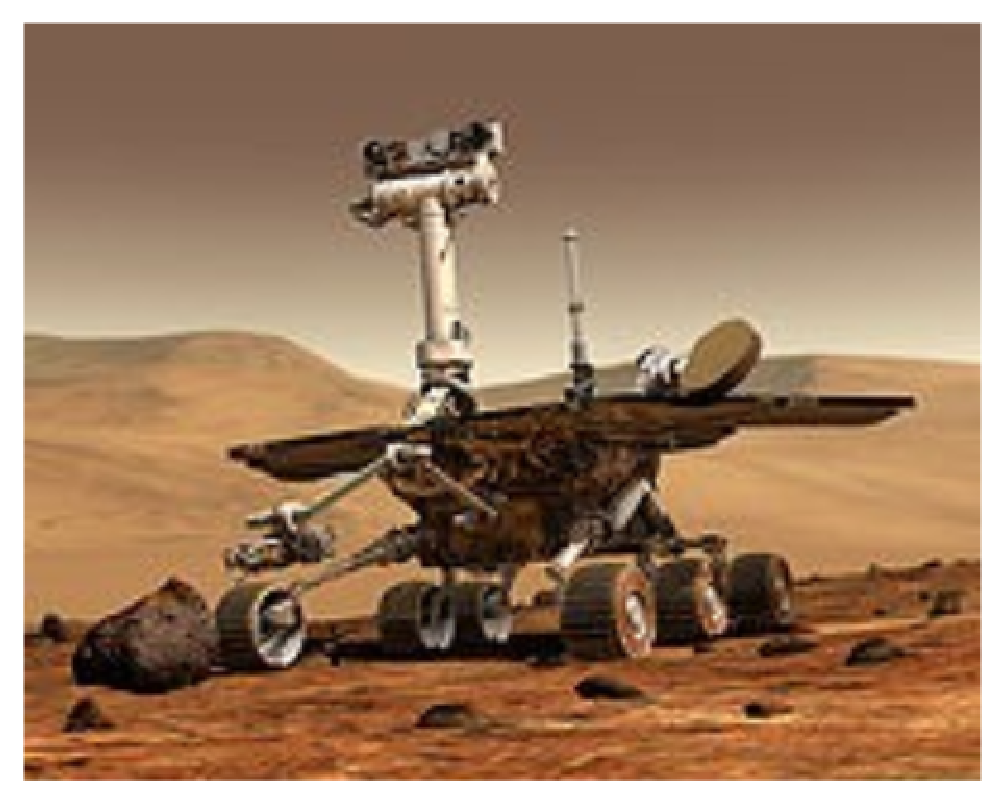
\includegraphics[width=\hsize]{mars-rover}
  \legend{Visão computacional em pesquisas interplanetárias na missão NASA/JPL Mars Exploration Rover (MER).}
  \source{Matthies et al. (2007).}
\end{figure}

A geometria projetiva é a principal teoria matemática usada em visão computacional tridimensional. Com a introdução de algumas definições e conceitos, a geometria projetiva pode ser estudada em termos de álgebra linear. Apesar de possuir algumas limitações, tal abordagem traz alguns benefícios de modelagem e é amplamente utilizada por pesquisadores dessa área. Em pesquisas recentes, Kuang e \AA str\"om (2013), verificou-se a eficácia do uso de técnicas de geometria algébrica em resoluções de sistemas de equações polinomiais, oriundos de problemas de visão computacional 3D. Fabbri e Kimia (2011) introduziram uma abordagem em termos de geometria diferencial, onde é possível aplicar o cálculo diferencial trabalhando diretamente com as equações algébricas. Essa abordagem permite um maior poder de modelagem matemática e computacional do espaço tridimensional através das imagens.

\section*{Motivação.}
As motivações para a pesquisa estão ligadas às suas aplicações em diversas áreas. A extração de informação da geometria 3D de um ambiente pode, por exemplo, ser utilizada na determinação da orientação e posição de veículos autônomos, para que os mesmos identifiquem a trajetória para os seus objetivos considerando a possibilidade de obstáculos. Um exemplo famoso, segundo Matthies et al. (2007) , é a aplicação em pesquisas interplanetárias onde foram usados algoritmos de visão computacional em veículos de exploração de Marte (Mars Exploration Rover - MER, em inglês), observado na Figura \ref{fig.mars-rover}.

Uma aplicação mais recente foi a reconstrução virtual de objetos, estátuas ou monumentos de valor histórico e cultural que foram destruídos pela ação do tempo ou do homem (possivelmente em guerras), através da aquisição de imagens em acervos ou na internet. Um exemplo é o Museu de Mosul {\footnote{Outros exemplos podem ser encontrados em http://www.projectmosul.org/}}, no Iraque, atacado pelo 
Estado Islâmico em 2015, que teve algumas de suas obras reconstruídas como podemos visualizar na Figura \ref{fig.mossul}.


\begin{figure}[!htb]{16cm}
\caption{O le\~ao de Mosul.}
\subfloat{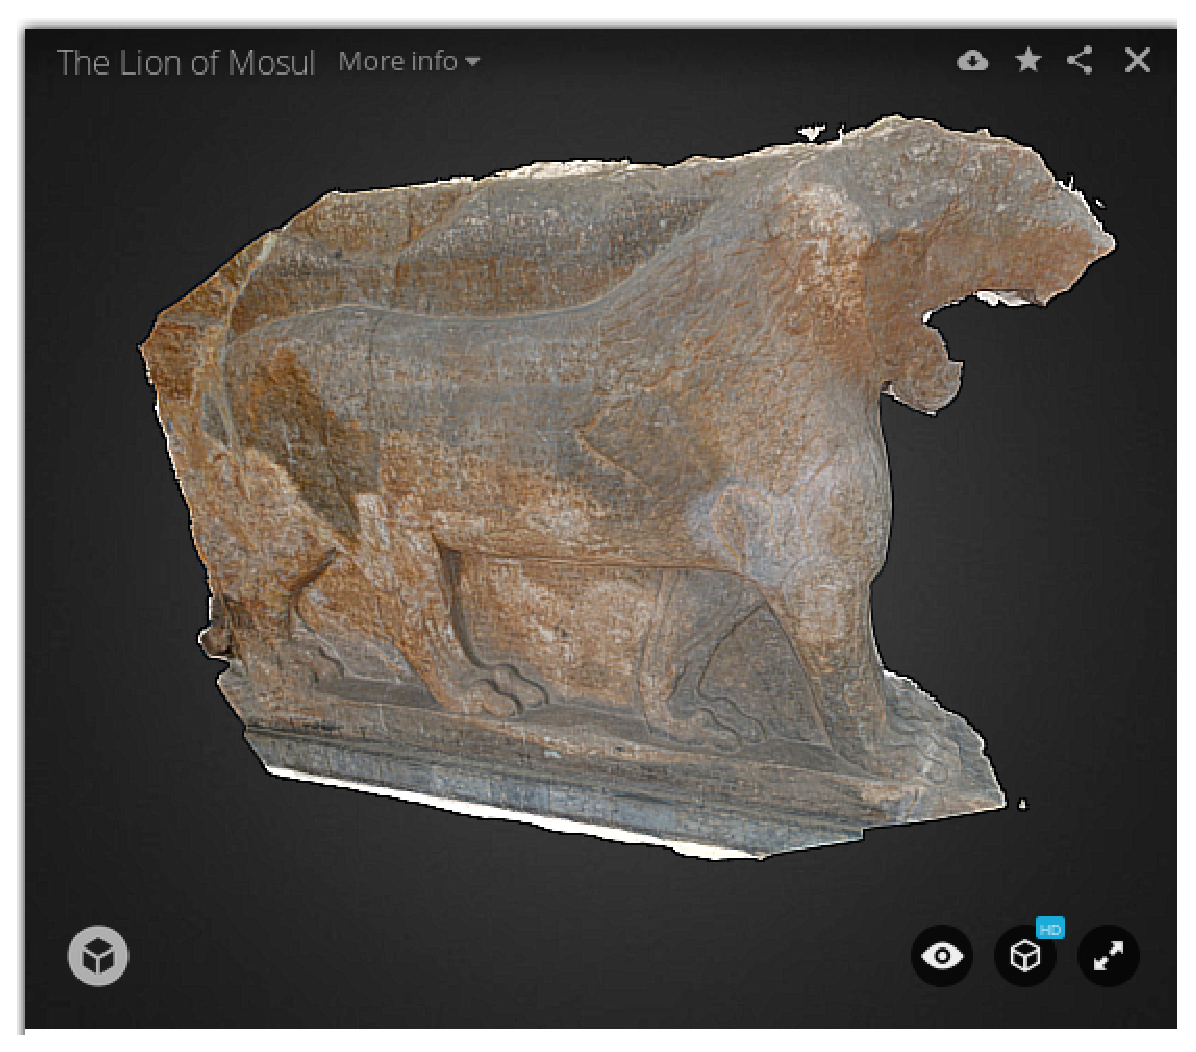
\includegraphics[width=0.45\hsize]{leao-mosul}}\hfill
\quad
\subfloat{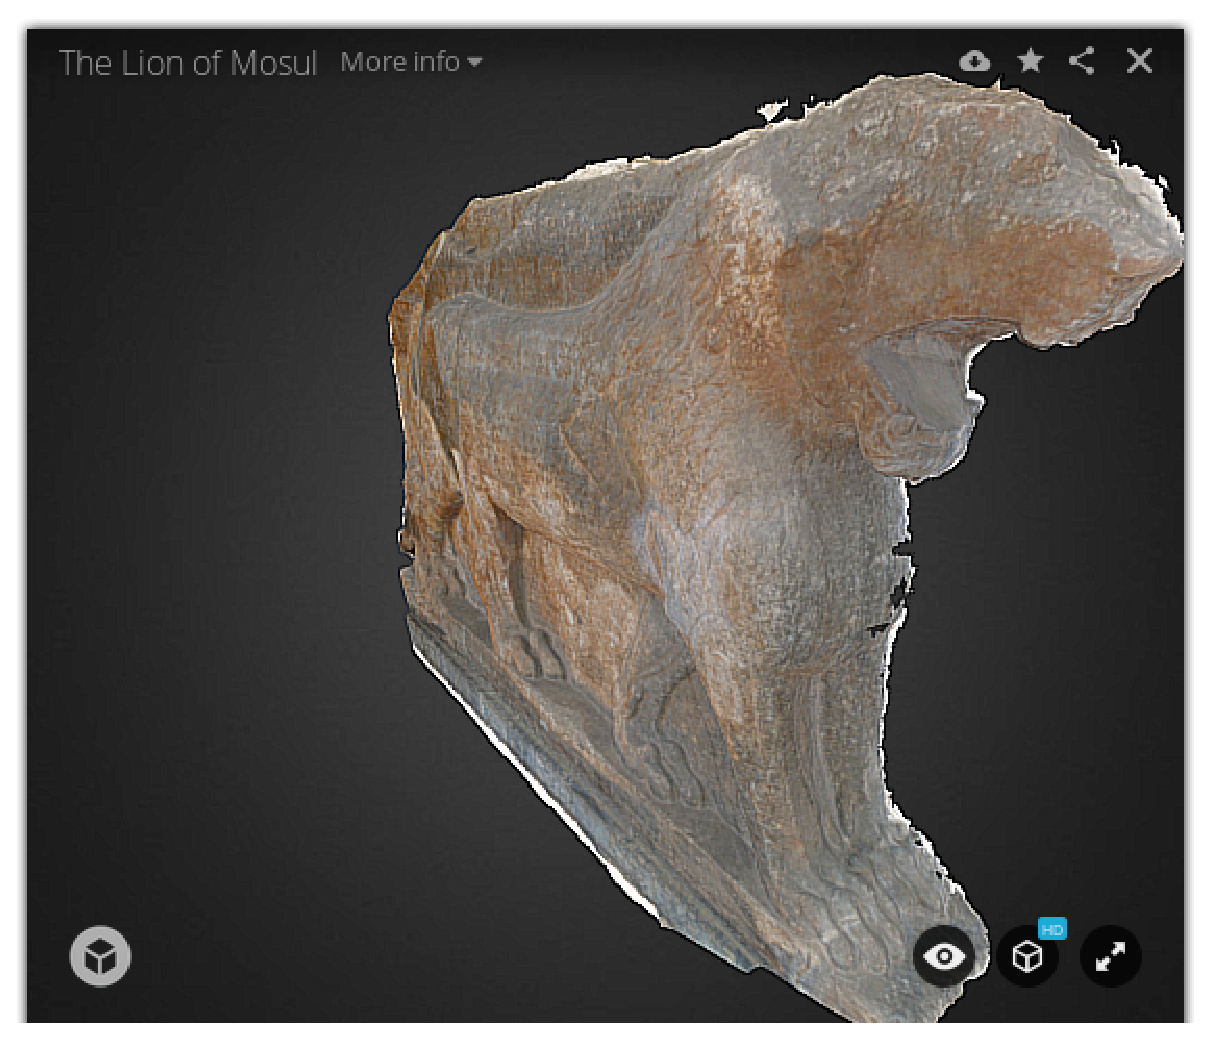
\includegraphics[width=0.47\hsize]{lion-mosul-2}}\hfill
\legend{A reconstrução do Leão de Mosul, um dos artefatos destruídos por extremistas religiosos em 2015 no Iraque.}
\label{fig.mossul}
\source{http://www.projectmosul.org/}
\end{figure}

As aplicações de visão computacional são bastante variadas, com pesquisas em outras áreas como astronomia, medicina e química. Para se ter uma ideia, Ballard e Brown (1982) já apresentavam imagens e tabelas com resumos de aplicações em oito áreas diferentes no início dos anos 1980.  

Novos avanços em reconstrução 3D vêm sendo realizados constantemente como observamos em Fabbri e Kimia (2015), que apresentam uma abordagem para a reconstrução de um desenho 3D (3D \emph{drawing} em inglês) de uma cena. Isto é, um conjunto de fragmentos de curvas em 3D interligadas de forma que preserve suas relações espaciais, capturadas em forma de gráficos a partir de um grande conjunto de dados multifocal. A ideia base é aprimorar uma abordagem anterior (3D curve \emph{sketch}) divulgada pelos mesmos autores, Fabbri e Kimia (2010a), conforme exemplo visualizado na Figura \ref{fig.drawing2}.
\begin{figure}[!htb]{\textwidth}
\caption{3D \emph{drawing}}
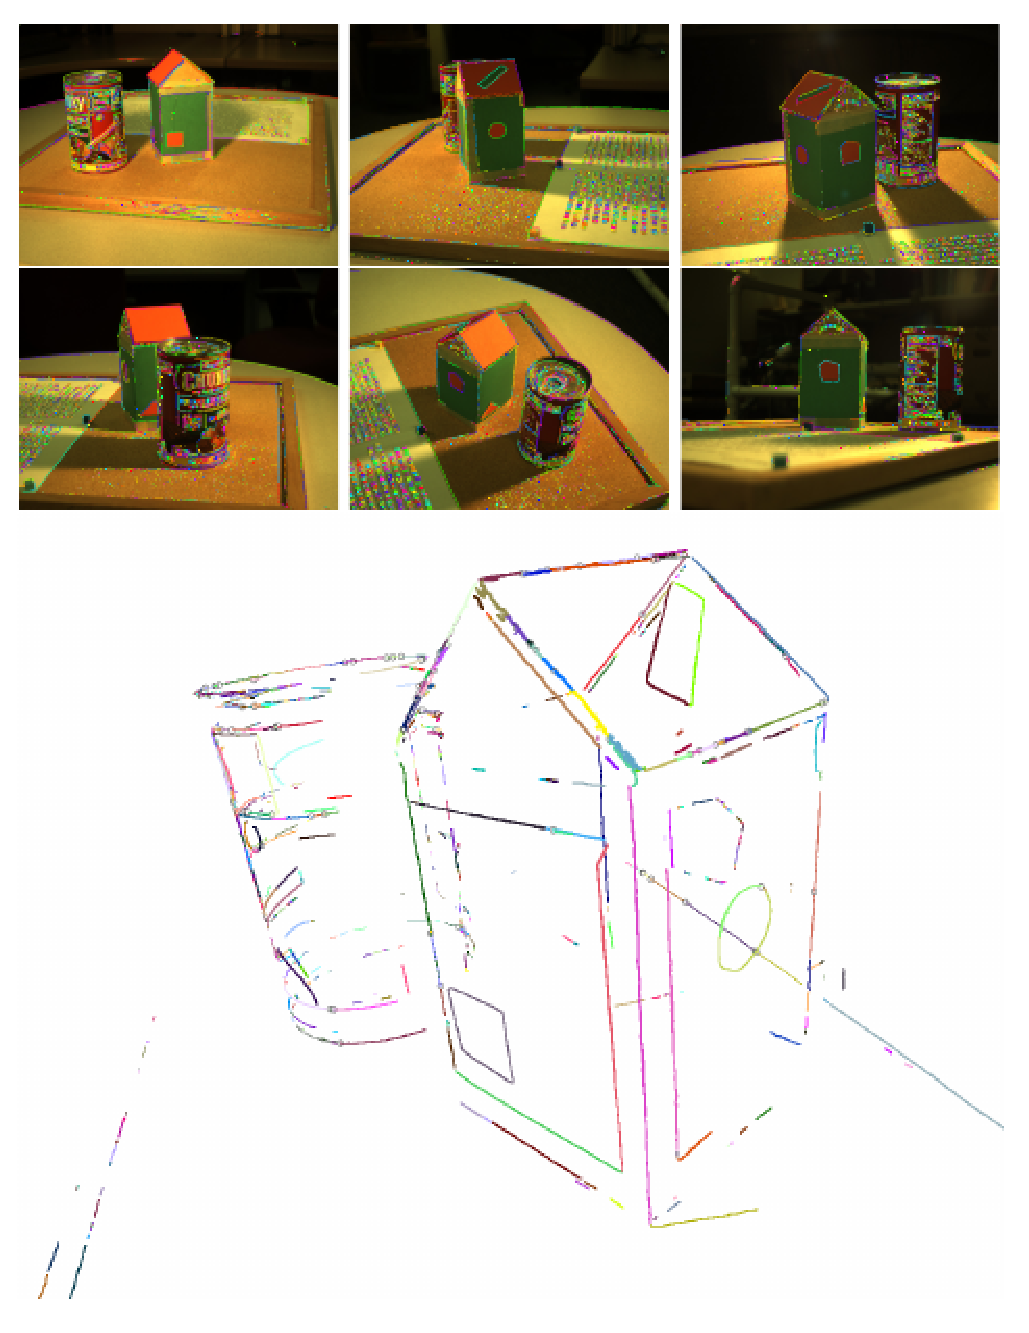
\includegraphics[width=\hsize]{drawing2}
\legend{A abordagem transforma um conjunto de imagens calibradas no desenho 3D, na forma de um gráfico consistindo de segmentos de curvas que se ligam nas junções.}
\source{Fabbri e Kimia (2015).}
\label{fig.drawing2}
\end{figure}
A maioria dos métodos de reconstrução não utilizam geometria diferencial de curvas, mas se baseiam em correlacionar pontos de interesse através das imagens e produzem uma desorganizada nuvem de pontos em 3D, Figura \ref{fig.medusa}. Tais métodos obtêm sucesso em ambientes controlados, com cenas em larga escala e imagens ricas em textura, mas não podem ser aplicados em configurações gerais. Não podem reconstruir superfícies suaves e homogêneas nem suas fronteiras devido a esparsidade de pontos de interesse, como também não podem reconstruir regiões que se alteram drasticamente com a mudança de luz ambiente. Exemplos de imagens sujeitas a essas limitações são dados na Figura \ref{fig.carro-objeto-curvo}.
\begin{figure}[!htb]{14cm}
\caption{Objetos com pouca textura.}
\subfloat{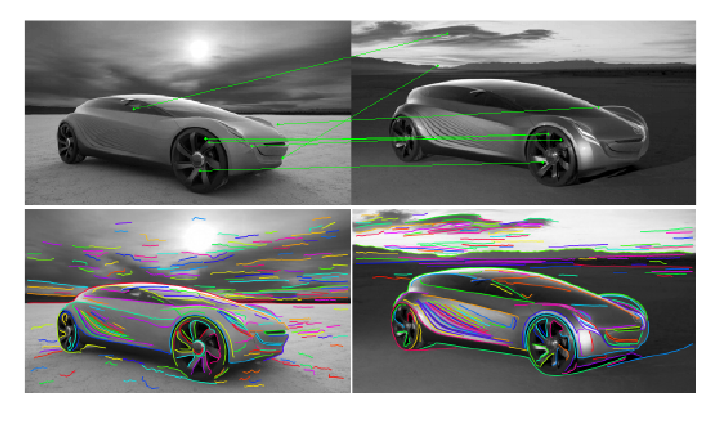
\includegraphics[width=.713\hsize]{carro}}\hfill
\subfloat{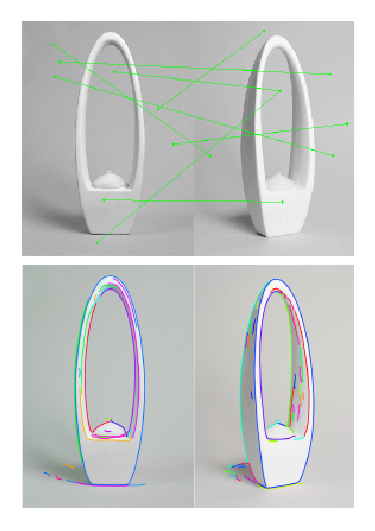
\includegraphics[width=.28\hsize]{objeto-curvo}}\hfill
\legend{Exemplos de objetos que não podem ser reconstruídos através da abordagem tradicional usando pontos de interesse e a geometria epipolar.}
\source{Fabbri et al. (2012).}
\label{fig.carro-objeto-curvo}
\end{figure}
Daí são utilizadas outras técnicas de melhoramento dos resultados, como a interpolação de pontos e texturização, mas que não fornecem um resultado plenamente satisfatório. Podemos ver as fases desse processo em um exemplo no conjunto de imagens na Figura \ref{fig.medusa}.

Portanto, ainda é necessário que se continuem as pesquisas em visão computacional, e o presente trabalho tem a finalidade de, primeiramente, detalhar as abordagens de artigos recentes na busca de novas combinações de ferramentas matemáticas que possam melhorar as atuais abordagens e atenuar o esforço computacional. Segundo, a verificação dos benefícios obtidos com o uso da geometria trifocal em transferência de pontos e reconstrução 3D em comparação com a geometria epipolar (mais usada atualmente), tudo com o objetivo de auxiliar na construção de uma nova abordagem usando geometria diferencial multifocal em condições realísticas.
\begin{figure}[!htb]{\textwidth}
\caption{M\'etodo tradicional de reconstru\c c\~ao.}
\subfloat{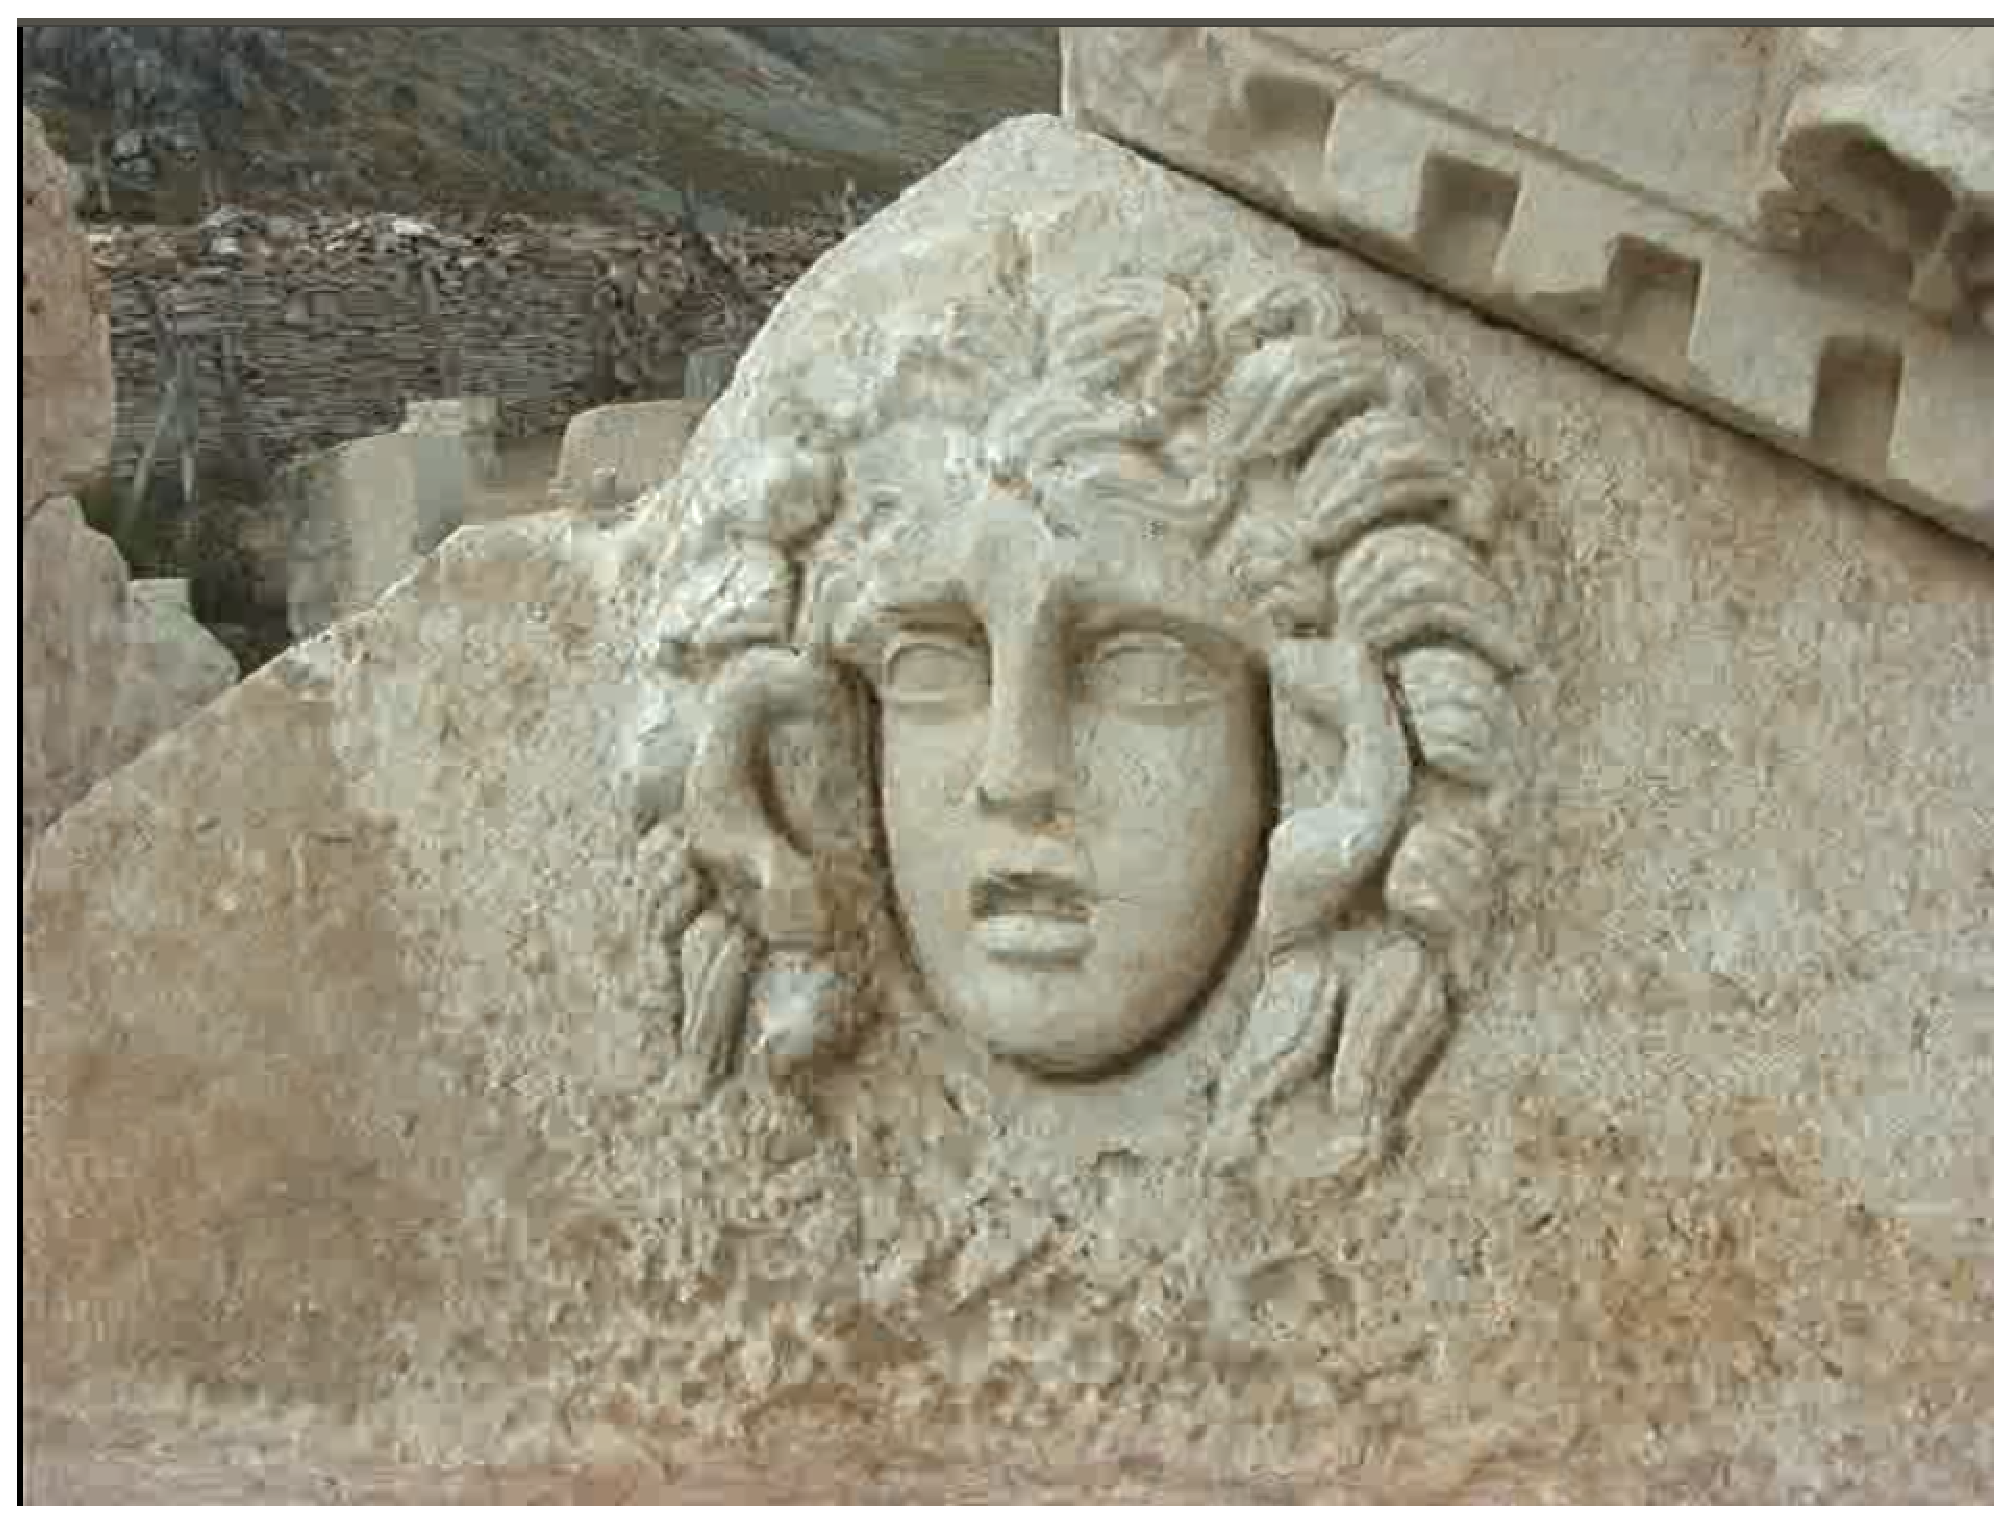
\includegraphics[width=.49\hsize]{medusa1}}\hfill
\subfloat{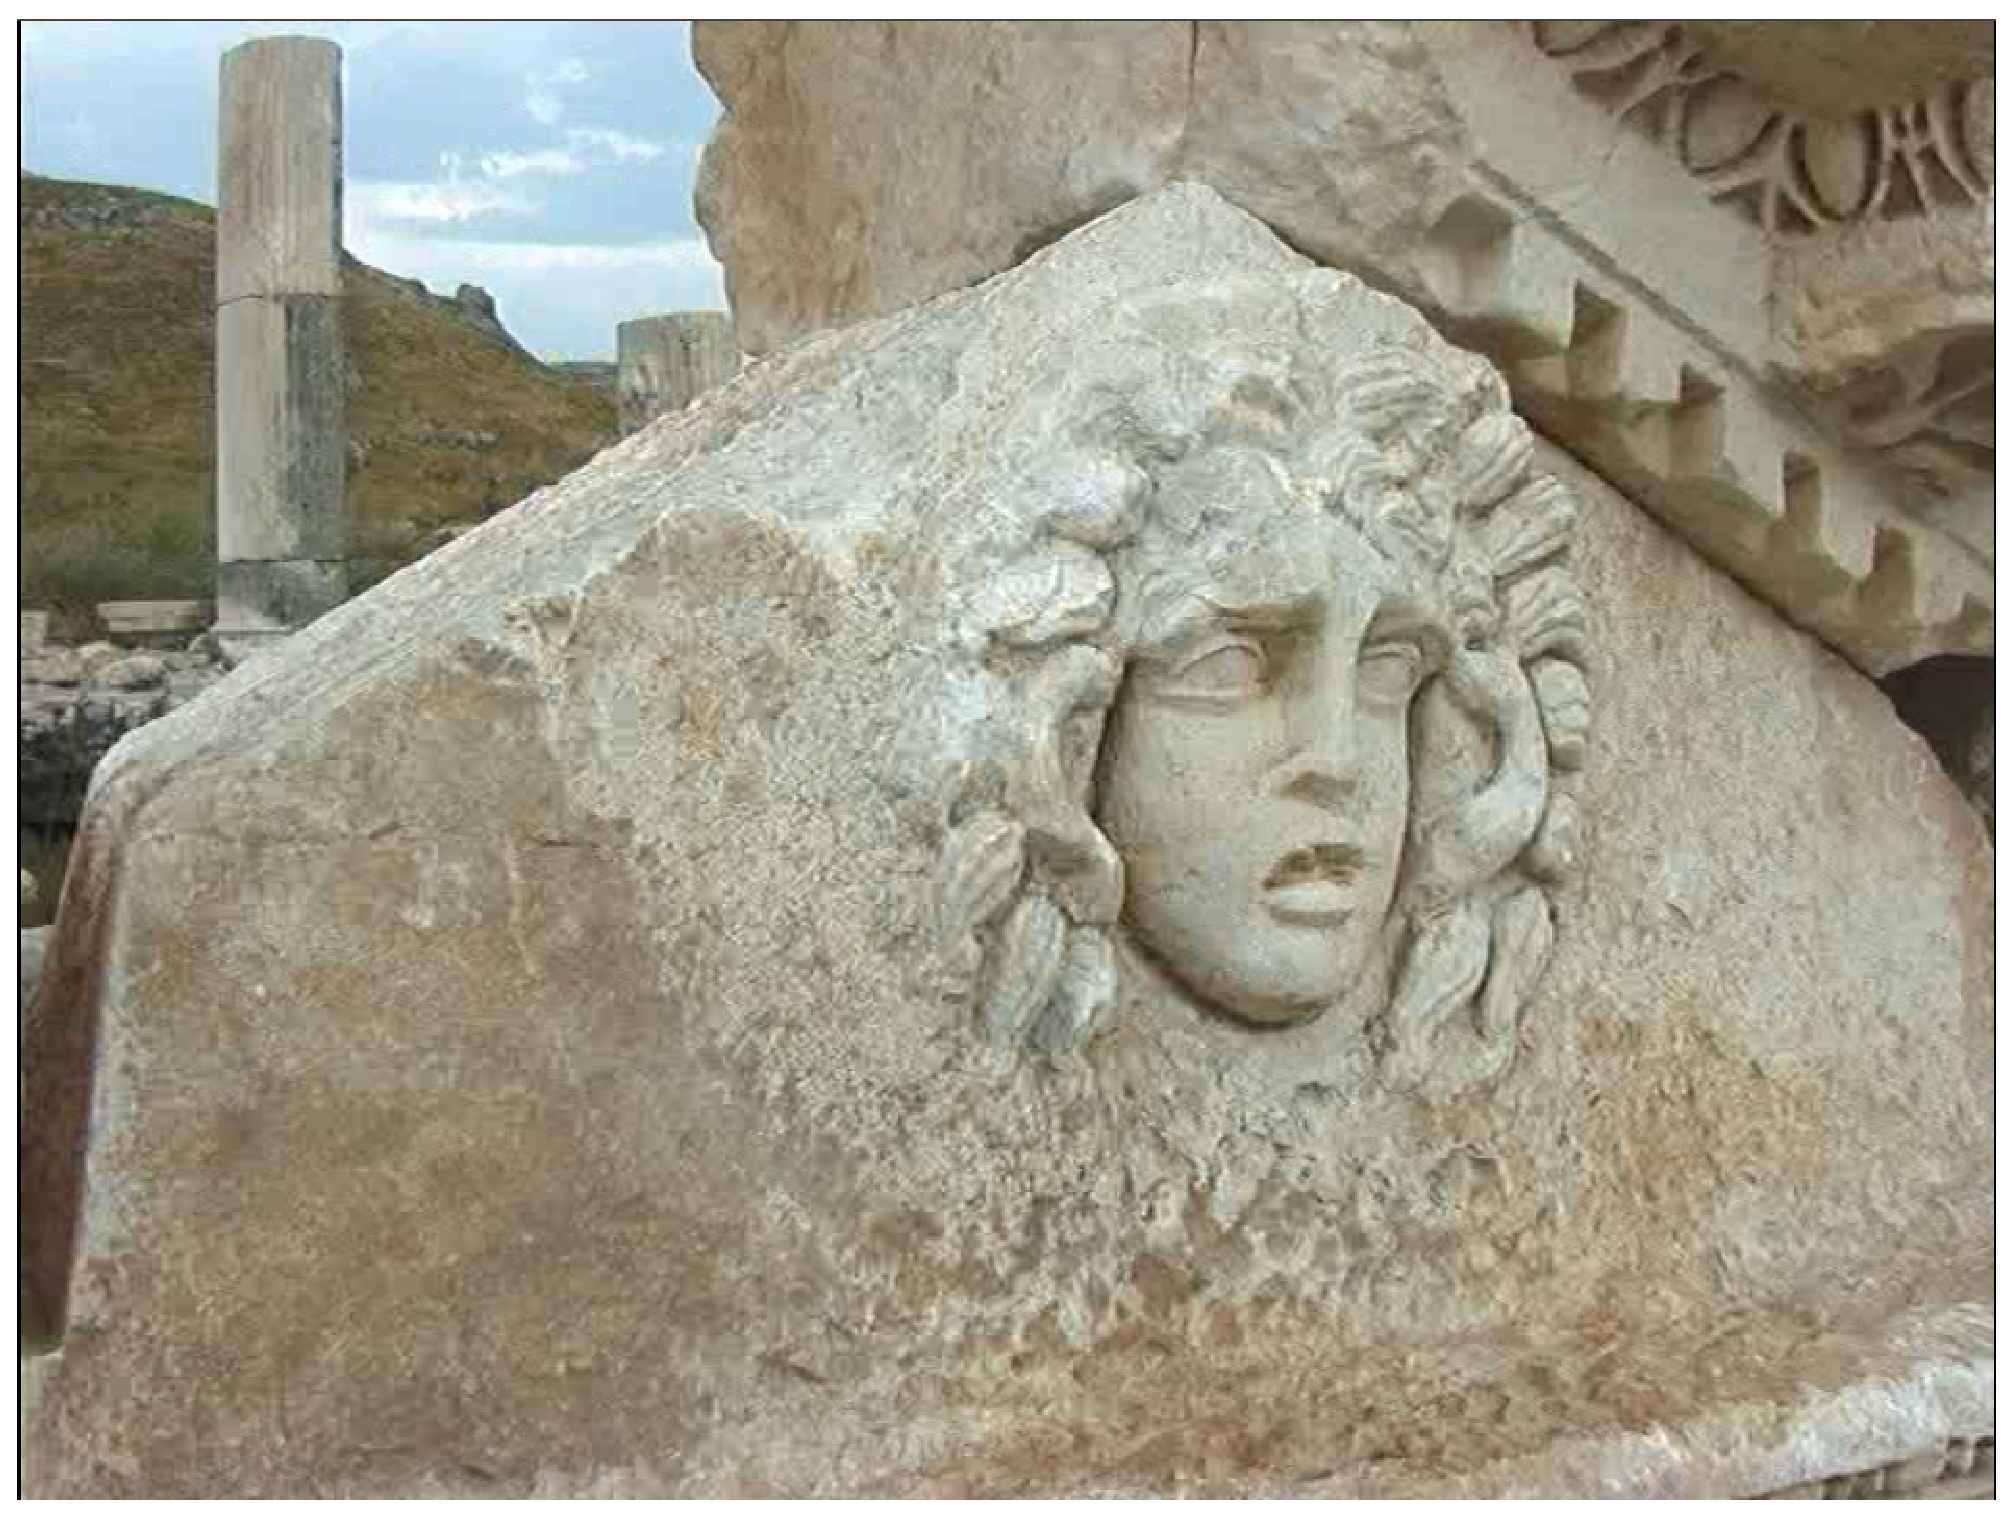
\includegraphics[width=.49\hsize]{medusa2}}\hfill
\\
\subfloat{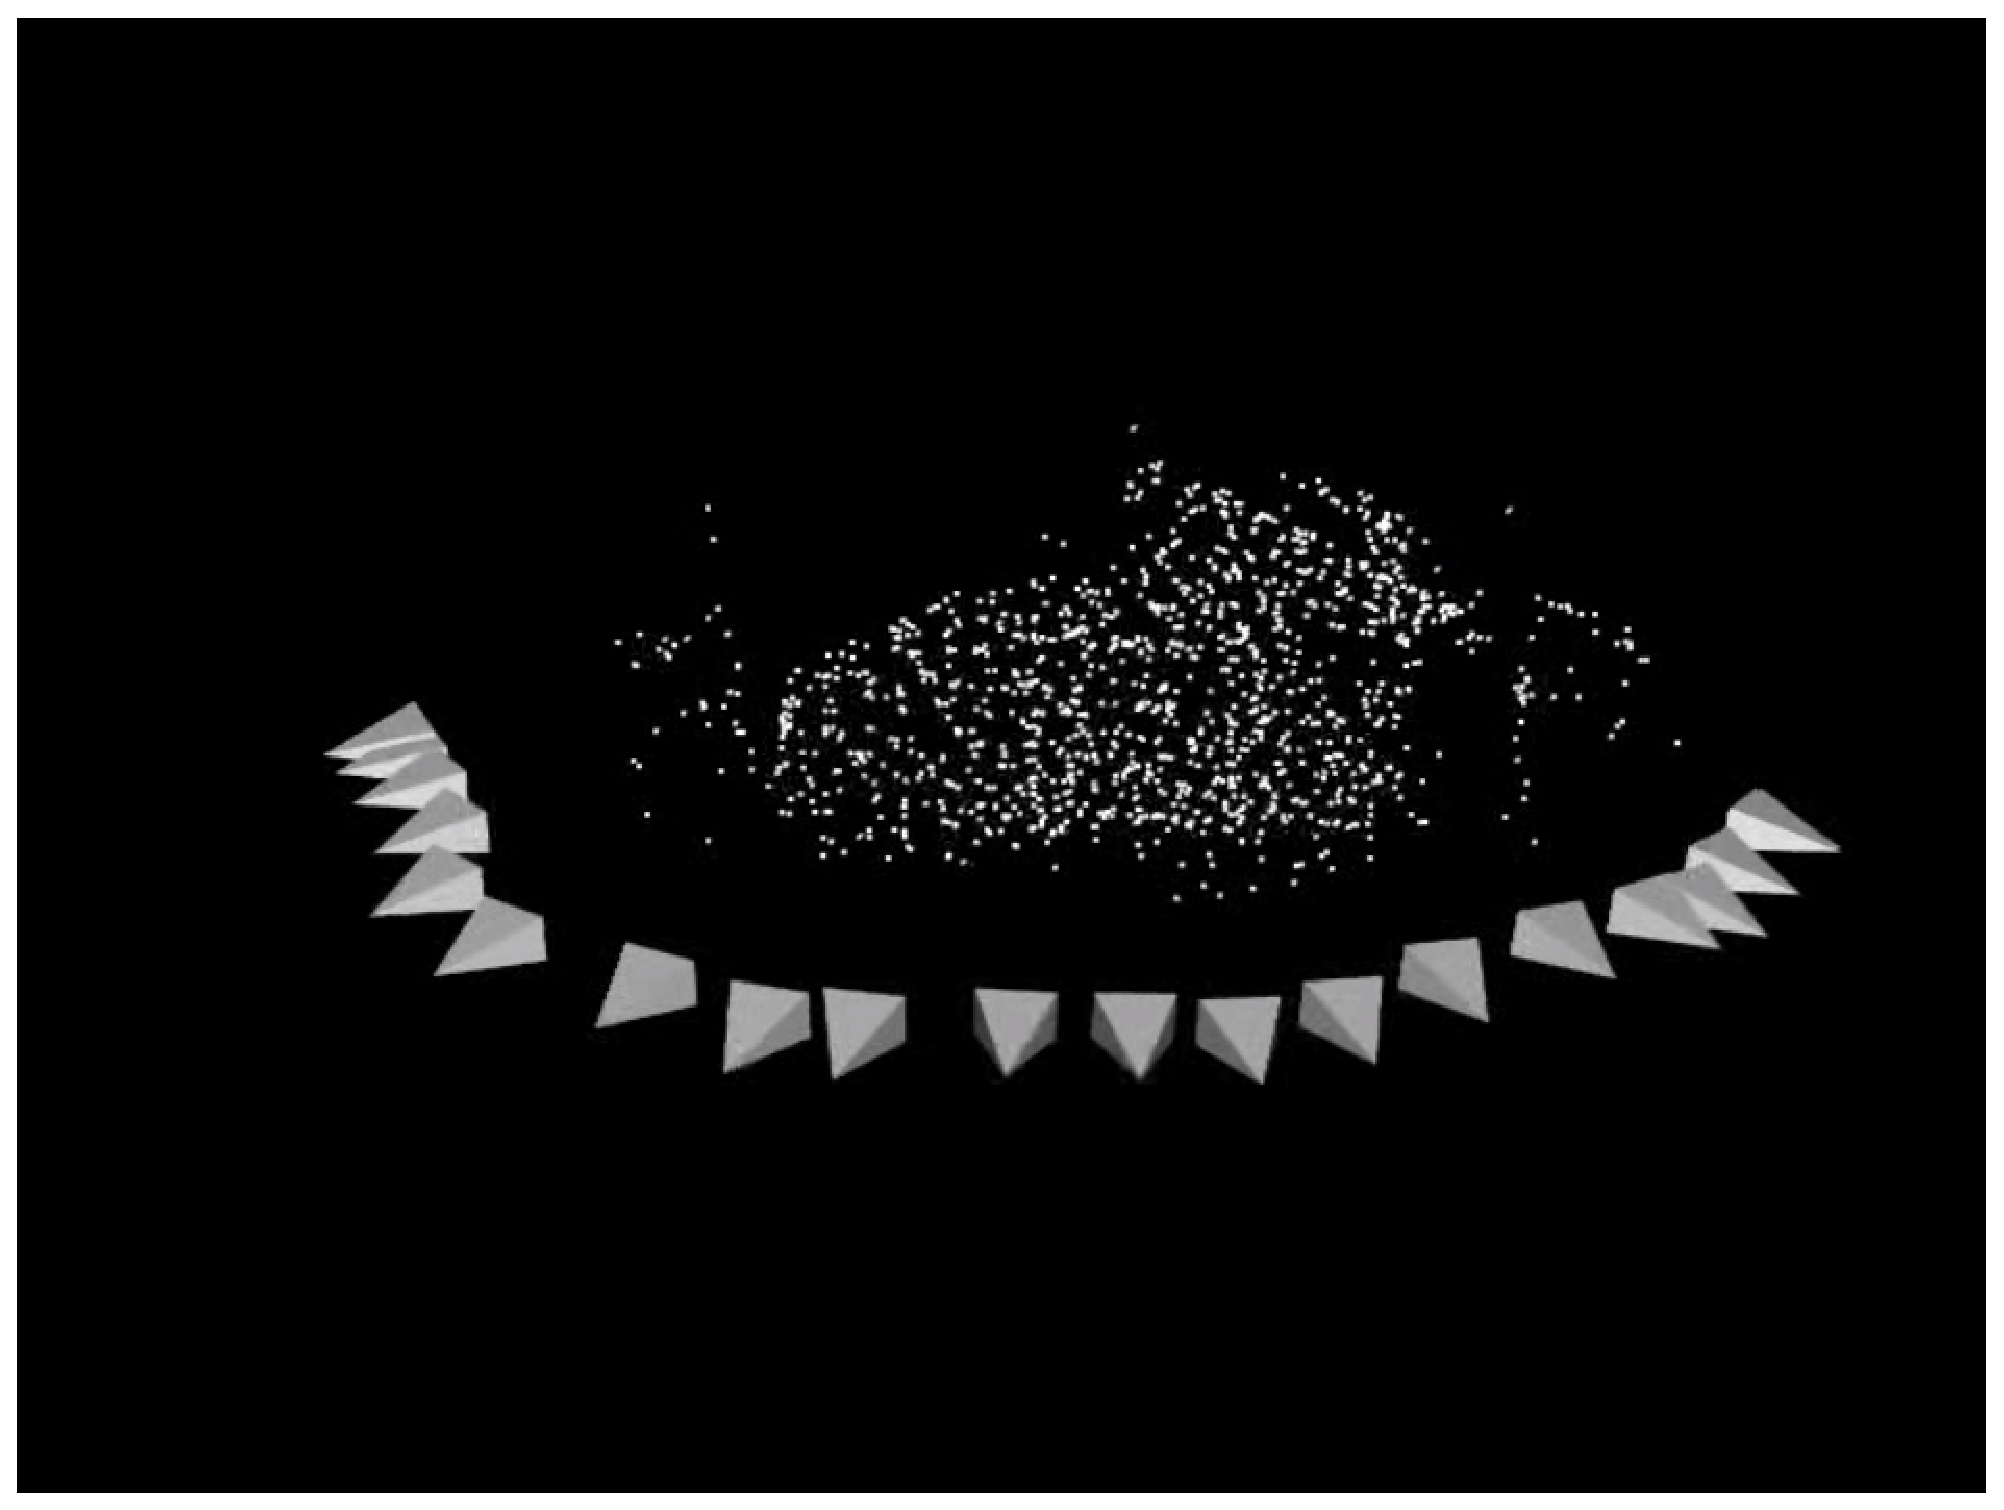
\includegraphics[width=.49\hsize]{nuvem1}}\hfill
\subfloat{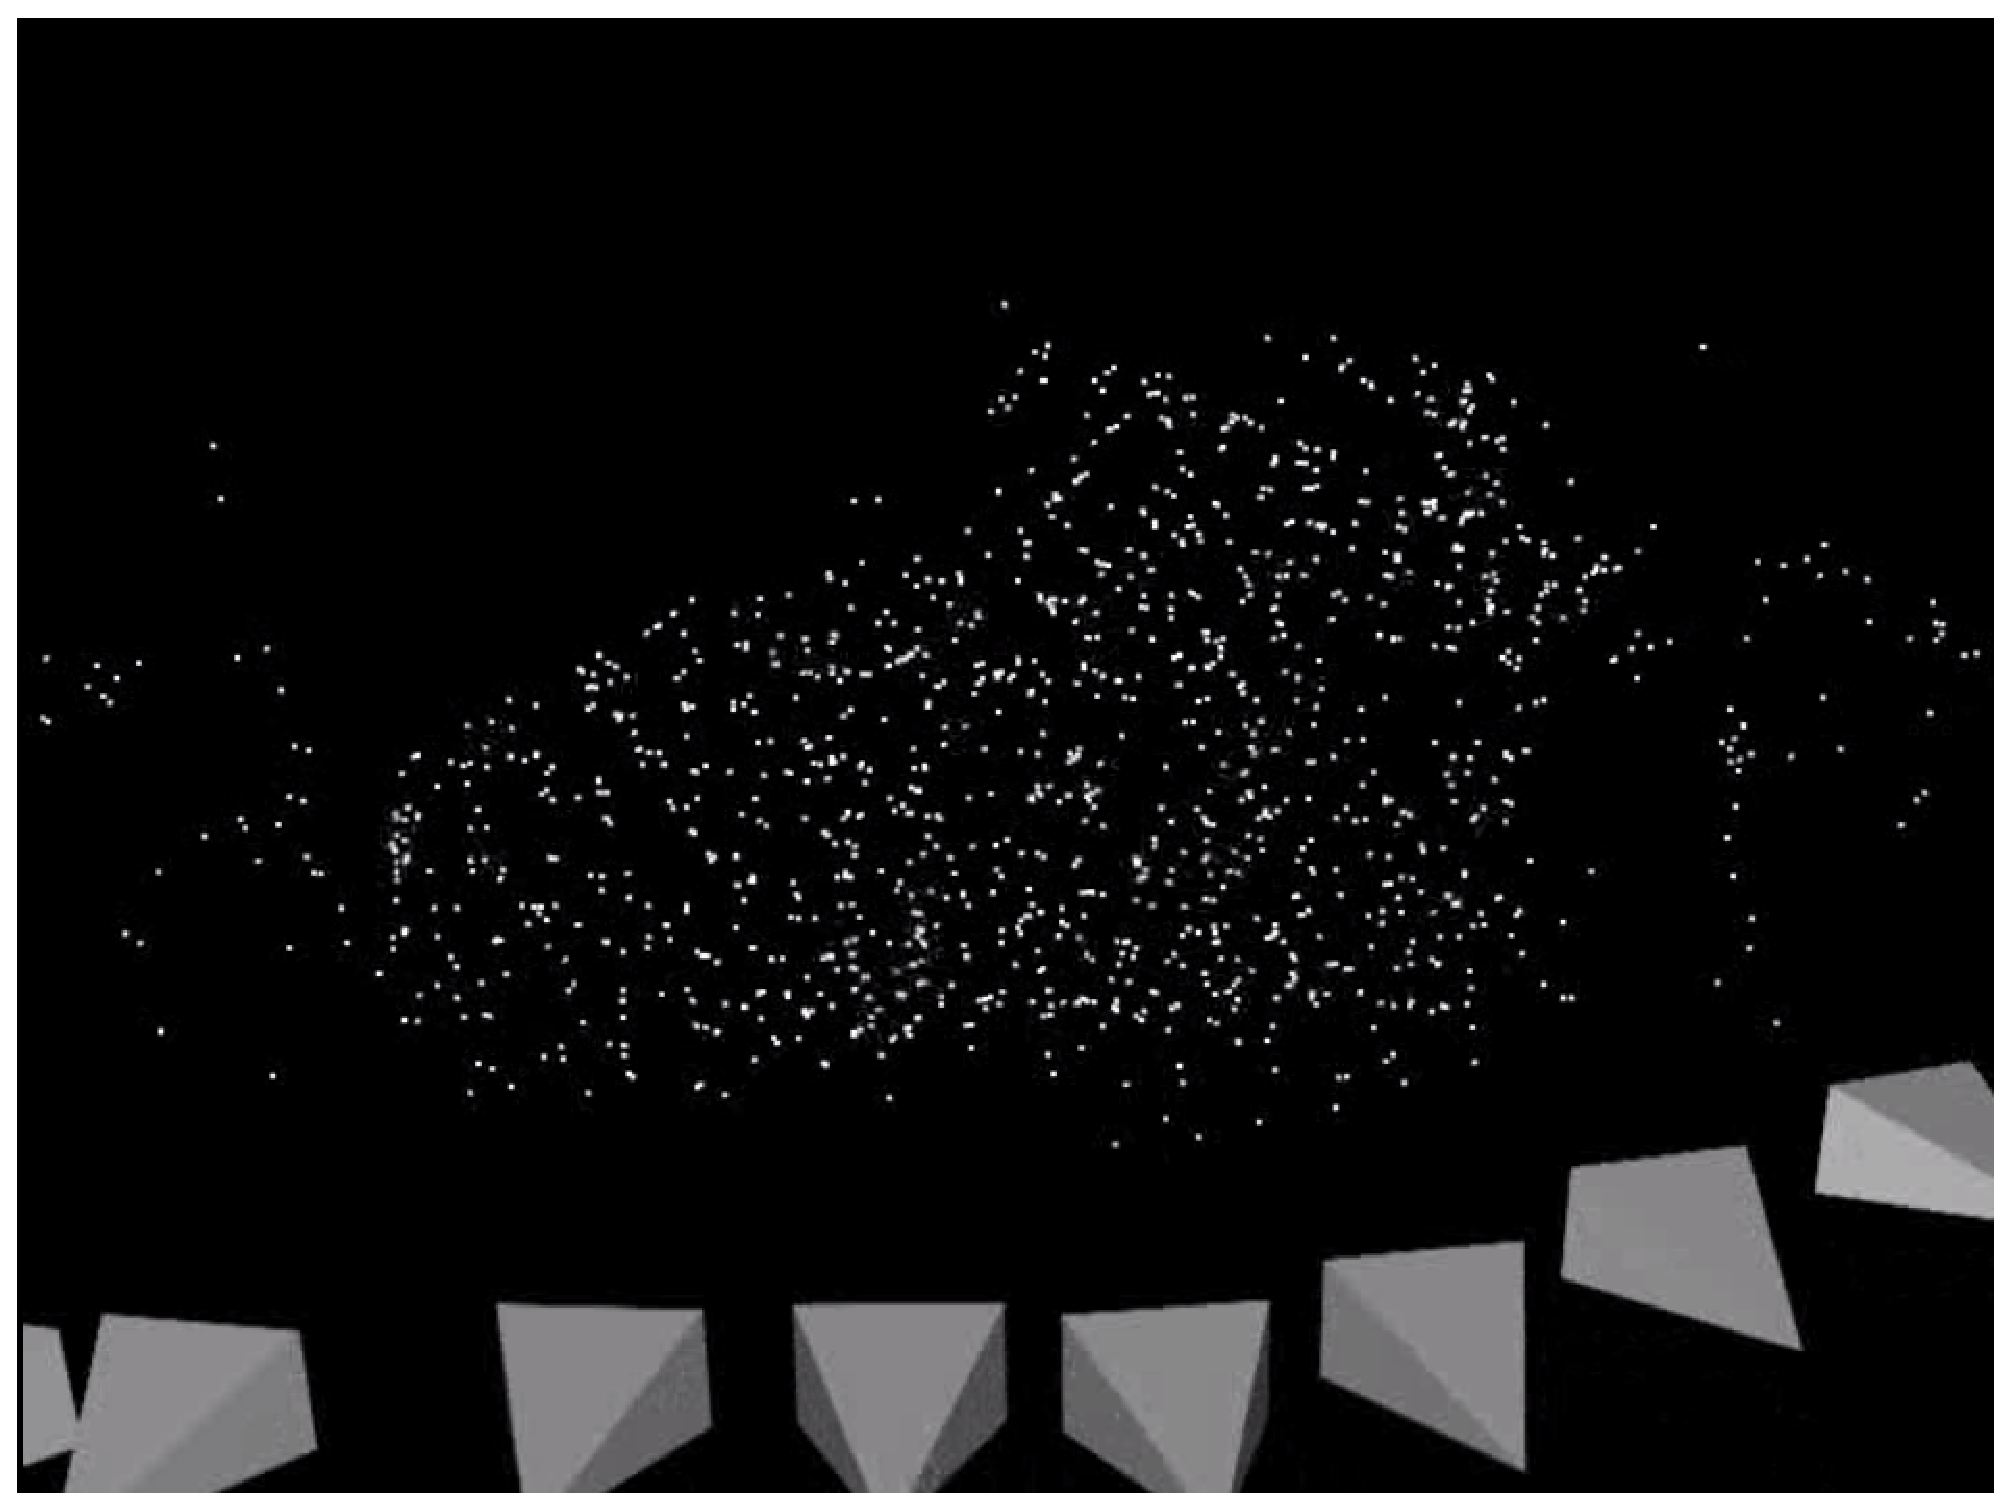
\includegraphics[width=.49\hsize]{nuvem2}}\hfill
\\
\subfloat{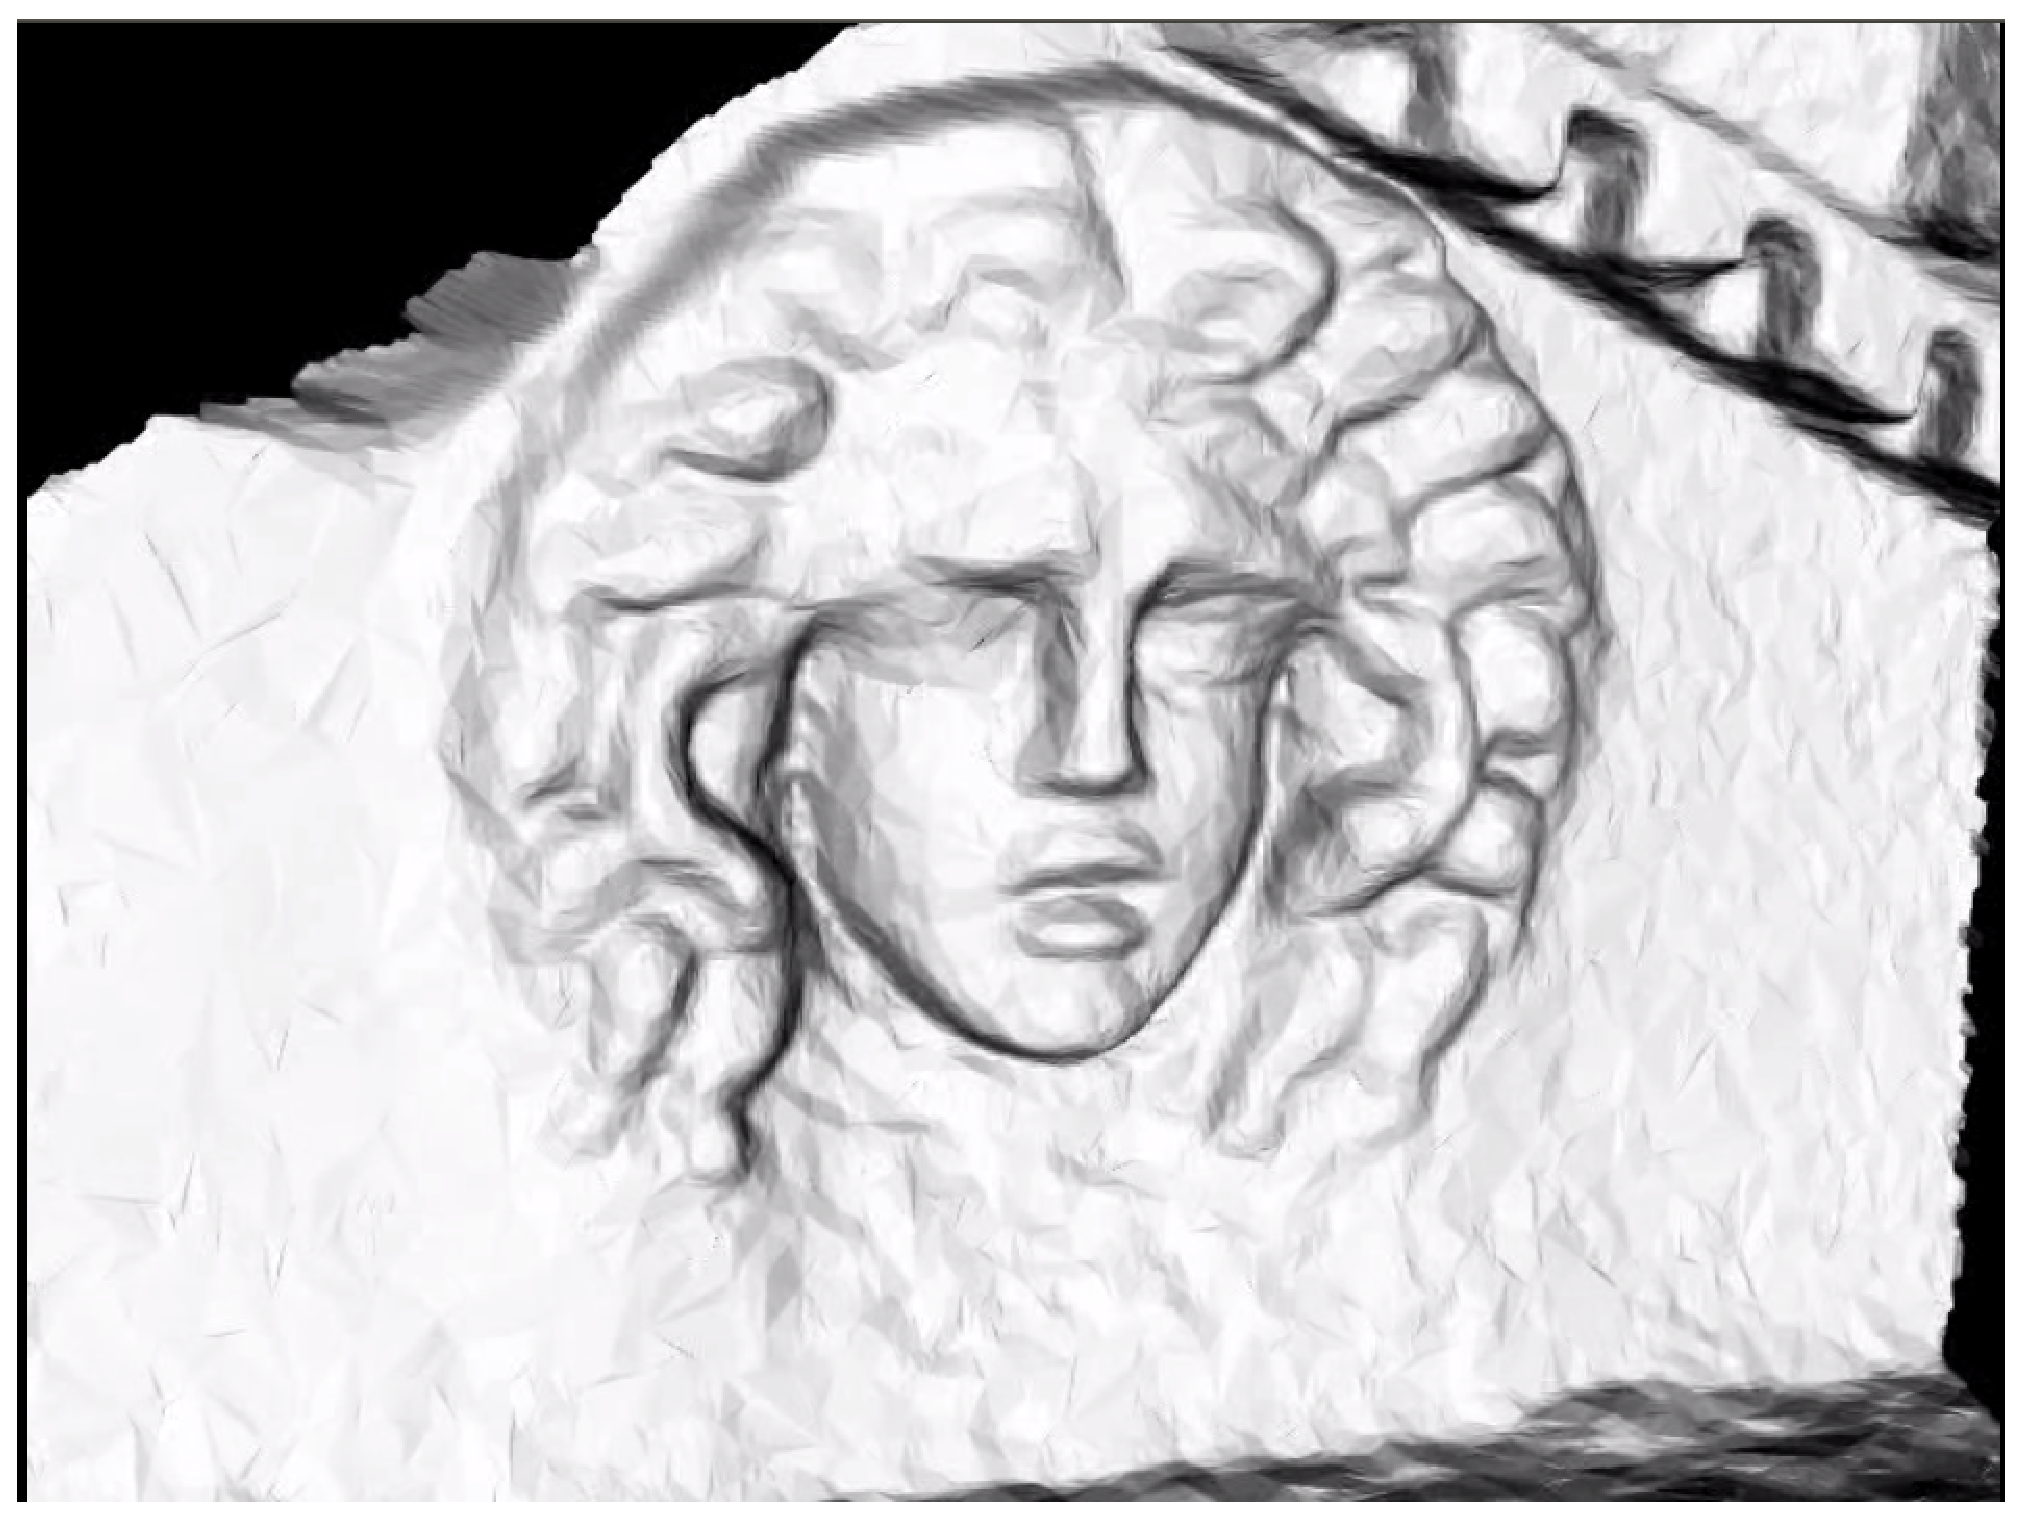
\includegraphics[width=.49\hsize]{texturizacao2}}\hfill
\subfloat{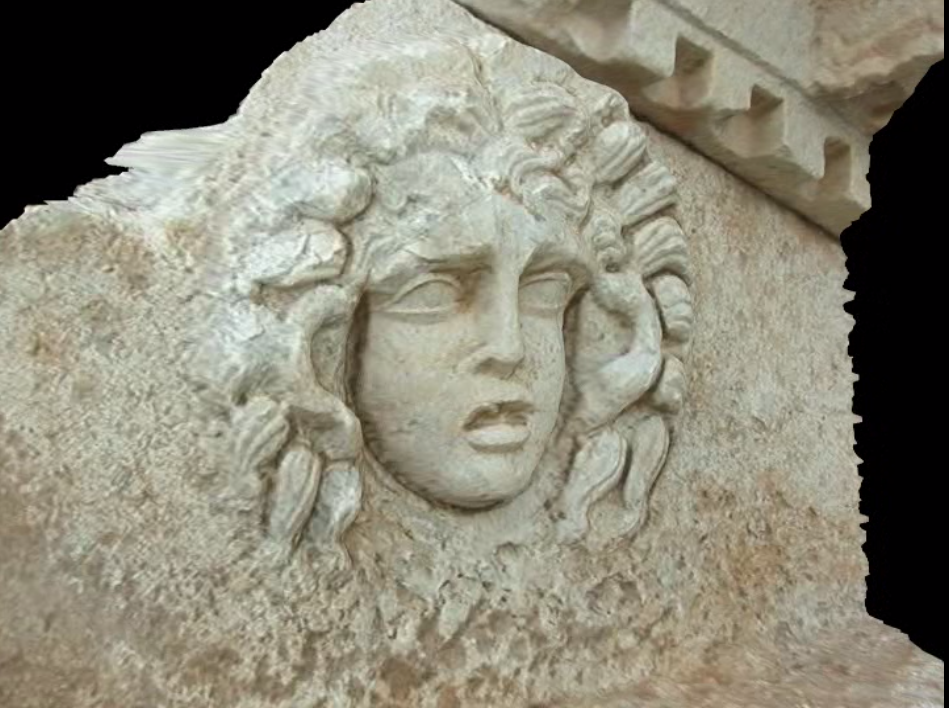
\includegraphics[width=.49\hsize]{texturizacao-realmente}}\hfill
\legend{Em cima, duas imagens extraídas de um vídeo (utilizado em reconstrução 3D) da estátua da Medusa em Sagalassos, Turquia. No meio, a nuvem de pontos obtida após a reconstrução 3D juntamente com as posições da câmera. Em baixo, aplicação de interpolação de pontos e texturização.}
\source{http://www.cs.unc.edu/~marc/research.html}
\label{fig.medusa}
\end{figure}

\section*{Visão geral e objetivos.}

A seção \ref{sec.geo-1-2-cam} engloba a teoria básica de geometria projetiva utilizada em visão computacional 3D, com abordagens em termos de álgebra linear e usando o tipo de notação mais difundido entre pesquisadores da área. Além dos conceitos básicos, também são apresentados alguns conceitos e definições um pouco mais avançados indispensáveis ao entendimento das demais seções da dissertação, tudo com a finalidade de facilitar a compreensão do leitor sem a necessidade de consulta em outras publicações. Em seguida, há a apresentação da geometria epipolar, num sistema de visão estéreo com duas câmeras, bem como extração da matriz fundamental e a reconstrução das câmeras, usando essa abordagem bifocal que é mais comum do que a abordagem trifocal.

Na seção \ref{sec.astrom} temos o detalhamento de um artigo recente e representativo para a reconstrução de uma câmera a partir de objetos geométricos em 3D e suas respectivas imagens em 2D, Kuang e \AA str\"om (2013). A importância dessa publicação se verifica na utilização dos quatérnions de Hamilton para a parametrização da matriz de rotação da câmera, pois desta forma a matriz que possui nove componentes é parametrizada com apenas quatro variáveis. Outra vantagem é utilização das bases de Gr\"obner e da matriz de ação para solução computacional de sistemas de equações polinomiais de grau elevado e com muitas variáveis.

A geometria trifocal e suas características são abordadas na seção \ref{sec.geo-tri}, juntamente com a descrição dos benefícios do uso dessa geometria num sistema com três câmeras em comparação com uso da geometria epipolar entre cada par de câmeras. Após as comparações são apresentados métodos para a extração das matrizes fundamentais e métodos de reconstrução das câmeras a partir do tensor trifocal.  

Na seção \ref{sec.nister} há o detalhamento matemático da abordagem mais eficiente, até a presente data, para a reconstrução 3D das câmeras num sistema trifocal calibrado, conforme Nist\' er e Schaffalitzky (2006). O artigo é bastante denso, com 25 teoremas, e apresenta a reconstrução de duas câmeras num sistema bifocal utilizando uma intrincada rede de conhecimentos de geometria projetiva. Depois da reconstrução das duas primeiras câmeras, é utilizada a reconstrução 3D de pontos para a reconstrução da terceira câmera, num procedimento similar ao apresentado na seção \ref{sec.astrom}, ou seja, os dois artigos quase se complementam. Esse trabalho deixa bem clara a dificuldade de se realizar a reconstrução num sistema com três imagens de quatro pontos 3D numa cena.

No apêndice \ref{sec.Apen-A} são fornecidas ferramentas de álgebra linear acompanhadas de algumas definições mais restritas à assimilação da dissertação. No apêndice \ref{sec.geo-algebrica} há uma breve introdução aos conceitos básicos de geometria algébrica seguidos da apresentação (informal e em termos de exemplos) de uma teoria para resolução de sistemas de equações polinomiais com várias variáveis.


\newpage
\chapter{Geometria de uma e duas câmeras}\label{sec.geo-1-2-cam}

\section{O espaço projetivo em duas dimensões}\label{sec.espaco-P2}

Para a compreensão mínima das técnicas mais importantes investigadas nessa dissertação, faz-se necessária a revisão condensada de um arcabouço notacional e conceitual que está disperso na literatura.

\subsection{A reta}\label{sec.reta}


Sabe-se que uma reta no plano $\mathbb{R}^{2}$ pode ser representada pela equação $a\,x+b\,y+c=0$, onde a reta fica perfeitamente determinada pelos valores das constantes $a$, $b$ e $c$. Desta forma, podemos representar retas através de vetores, e assim a reta $a\,x+b\,y+c=0$ seria representada por $\lightrgb = (a,b,c)^\top \in \mathbb{R}^{3}$, utilizando o símbolo em negrito $\lightrgb$ para indicar tal vetor escrito em coluna, por padrão. Nota-se que a relação entre uma dada reta e o seu respectivo vetor não é biunívoca, pois o vetor $k\,(a,b,c)^\top$, tal que $k\neq 0$, representa a reta $k\,a\,x+k\,b\,y+k\,c=0$ que é a mesma reta $a\,x+b\,y+c=0$. Temos, então, infinitos vetores que representam uma mesma reta e formam uma {\it classe de equivalência}, onde essa classe pode ser representada por qualquer um de seus vetores. Os vetores de uma classe de equivalência, definida pela multiplicação por um escalar, são conhecidos como vetores {\it homogêneos}. O conjunto de classes de equivalência de vetores em $\mathbb{R}^{3} - (0,0,0)^\top$ forma o {\it Espaço Projetivo} $\mathbb{P}^{2}$. O vetor $(0,0,0)^\top$ foi excluído por não representar reta alguma. Após essas considerações, dizemos que uma reta no plano projetivo é representada pelo vetor $(a,b,c)^\top$ em {\it coordenadas homogêneas}.\\
\subsection{O ponto}\label{sec.ponto}
Sabemos que em $\mathbb{R}^{2}$ os pontos são representados através de pares ordenados do tipo $(x,y)$, e assim cada ponto pode ser identificado como um vetor $(x,y)^\top$. Os vetores em coordenadas homogêneas que se referem a pontos serão representados pelo símbolo em negrito $\x$, configurando uma terceira dimensão cuja coordenada é 1. Desse jeito, $\x=(x,y,1)^\top$. Sabemos também que um ponto $(x,y)$ pertence a uma reta $(a,b,c)^\top$ se, e somente se, $a\,x+b\,y+c=0$, ou, matricialmente:
\begin{equation*}
(x,y,1)^\top 
\begin{pmatrix}
 a  \\ 
 b  \\ 
 c 
 \end{pmatrix} 
 = 0 \qquad 
 \text{ou} 
 \qquad \x ^\top\lightrgb = 0.
\end{equation*}
Ou seja, temos um ponto de $\mathbb{R}^{2}$ representado como um vetor com três coordenadas. Observe que para $k\neq 0$, temos:
\begin{equation*}
(k\,x,k\,y,k)^\top 
\begin{pmatrix}
 a  \\ 
 b  \\ 
 c 
 \end{pmatrix} 
 = 0
 \qquad \Leftrightarrow \qquad
 (x,y,1)^\top
\begin{pmatrix}
 a  \\ 
 b  \\ 
 c 
 \end{pmatrix} 
 = 0.
\end{equation*}
Portanto,  variando $k$, podemos considerar os vetores em coordenadas homogêneas $(k\,x,k\,y,k)^\top \in \mathbb{P}^2$, como representantes do mesmo ponto $(x,y) \in \mathbb{R}^2$, e podemos resgatar nossa representação original aplicando o procedimento $(x/k,y/k)^\top$, pois $k \ne 0$.
\begin{figure}[!htb]{.8\textwidth}
\caption{Plano projetivo $\mathbb{P}^2$.}
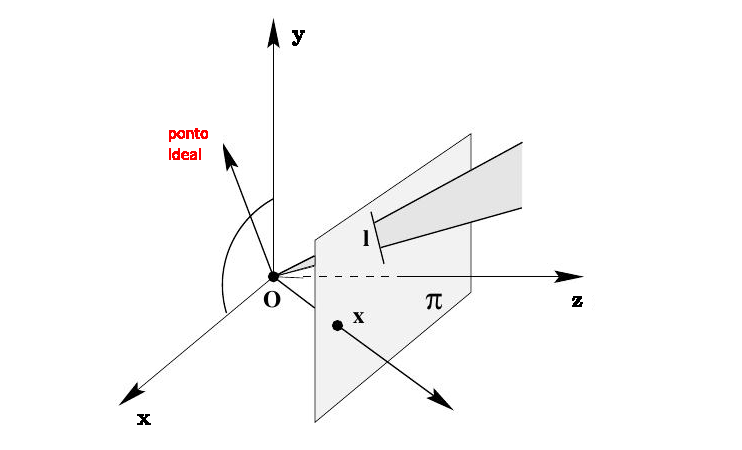
\includegraphics[width=\hsize]{espaco_P2}
\legend{O plano $\bpi$ representa o espaço projetivo $\mathbb{P}^2$. Pontos e retas pertencentes a esse espaço são representados, respectivamente, por vetores e planos que passam pela origem do $\mathbb{R}^3$. O ponto ideal é representado por um vetor que pertence ao plano $x\,y$, o qual é paralelo ao plano $\bpi$. O plano $x\,y$ representa a reta no infinito.}
\source{Adaptado, Hartley e Zisserman (2004).}
\label{plano_P2}
\end{figure}
Geometricamente, podemos pensar no plano projetivo como um conjunto de retas passando pela origem do $\mathbb{R}^3$, onde cada reta representa um único ponto, que é a interseção dessa reta com o plano $\mathbb{P}^2$. Analogamente, retas em $\mathbb{P}^2$ são formadas pela interseção de $\mathbb{P}^2$ com planos em $\mathbb{R}^3$. Na Figura \ref{plano_P2}, observamos como a interseção da reta com o plano define um ponto, assim como a interseção de dois planos definem uma reta. Inclu\'imos na representação o ponto ideal $(x,y,0)^\top$ e a reta no infinito que serão definidos mais adiante.


Como a representação de um ponto ou uma reta por vetores em coordenadas homogêneas não é alterada pela multiplicação por um escalar,  para determinarmos um ponto ou uma reta precisamos apenas de duas componentes do vetor, pois a terceira componente pode ser configurada como escala. Assim, dizemos que um ponto ou uma reta tem dois graus de liberdade.
\section*{Retas determinadas por dois pontos e a interseção de duas retas.}

A representação de retas em coordenadas homogêneas nos permite calcular a interseção de duas retas usando o produto vetorial. Sabemos que o produto vetorial de dois vetores, digamos $\lightrgb\times\lightrgb'$ em $R^3$ resulta num terceiro vetor que é ortogonal ao plano definido pelos vetores $\lightrgb$ e $\lightrgb'$. Em particular, esse terceiro vetor $\lightrgb\times\lightrgb'$ será ortogonal a qualquer dos vetores $\lightrgb$ e $\lightrgb'$, assim seu produto escalar é zero
\begin{equation*}
\lightrgb\cdot(\lightrgb\times\lightrgb')=\lightrgb'\cdot(\lightrgb\times\lightrgb')=0.
\end{equation*}
O produto escalar também pode ser representado por multiplicação matricial,
\begin{equation}\label{eq.pro-vet}
\lightrgb^\top(\lightrgb\times\lightrgb')=\lightrgb'^\top(\lightrgb\times\lightrgb')=0,
\end{equation}
e sendo $\x$ o ponto de interseção entre as duas retas temos
\begin{equation}\label{eq.pro-vet-2}
\lightrgb^\top\x=\lightrgb'^\top\x=0
\end{equation}
onde, comparando \ref{eq.pro-vet} e \ref{eq.pro-vet-2},
\begin{equation*}
\x=\lightrgb\times\lightrgb'.
\end{equation*}
Com argumento análogo podemos constatar que dois pontos definem uma reta através do produto vetorial entre eles, pois basta verificar que dois pontos $\x$ e $\x'$ pertencem a reta definida por
\begin{equation*}
\lightrgb=\x\times\x'.
\end{equation*}\\

\noindent {\bf Pontos ideais e a reta no infinito.}

Duas retas paralelas no espaço Euclidiano têm equações
\begin{equation*}
a\,x+b\,y+c=0\qquad\text{e}\qquad a\,x+b\,y+c'=0
\end{equation*}
com coordenadas homogêneas
\begin{equation*}
\lightrgb=(a,b,c)^\top\qquad\text{e}\qquad\lightrgb'=(a,b,c')^\top.
\end{equation*}
Computando a interseção entre as duas retas e ignorando o fator de escala $(c'-c)$ temos
\begin{equation*}
\begin{array}{rcl}
\lightrgb\times\lightrgb'&=&(a,b,c)^\top\times(a,b,c')^\top\\
&=&(c'-c)\,(b,-a,0)^\top\\
&=&(b,-a,0)^\top,
\end{array}
\end{equation*}
e se tentarmos encontrar as coordenadas não homogêneas do ponto de interseção temos
\begin{equation*}
\left(\frac{b}{0},\frac{-a}{0}\right)^\top,
\end{equation*}
o que não faz sentido matematicamente mas sugere que o ponto tem coordenadas que tendem ao infinito. Vetores homogêneos $(x,y,z)^\top$ com $z\neq0$ correspondem a pontos finitos em $R^2$ e, se $z=0$, os pontos são conhecidos como \textit{pontos ideais} ou \textit{pontos no infinito} no plano projetivo.

Se tomarmos um ponto no infinito genericamente $\x=(x,y,0)^\top$ percebemos que ele pertence a uma determinada reta $\lightrgb_\infty=(0,0,1)^\top$, pois
\begin{equation*}
\lightrgb_\infty^\top \x=(0,0,1)
\begin{pmatrix}
x\\
y\\
0
\end{pmatrix}
=0,
\end{equation*} 
e tal reta é conhecida como \textit{reta no infinto}. Assim, no plano projetivo temos que retas paralelas se encontram em ponto no infinito e o conjunto de pontos no infinito constituem a reta no infinito.

Um fato interessante sobre pontos no infinito é que eles são as direções das retas no plano projetivo $\mathbb{P}^2$. Um feixe de retas paralelas, que se intersectam num mesmo ponto no infinito, têm a mesma direção. Observa-se que a interseção de uma reta qualquer $\lightrgb=(a,b,c)^\top$ com a reta no infinito $\lightrgb_\infty=(0,0,1)^\top$,
\begin{equation*}
\lightrgb\times \lightrgb_\infty=(b,-a,0),
\end{equation*}
é um vetor que, em coordenadas não homogêneas $(b,-a)$, é ortogonal ao vetor $(a,b)$, que é o vetor normal à reta dada $\lightrgb=(a,b,c)^\top$. Assim $(b,-a)$ constitui-se a direção da reta $\lightrgb$, e como a reta no infinito contém todos os pontos do tipo $(b,-a,0)$, dizemos que a reta no infinito é o conjunto de direções das retas no plano projetivo $\mathbb{P}^2$.
\subsection{A cônica}\label{sec.definicao-conica}


Em Geometria Euclidiana, as cônicas são de três tipos principais: elipse, hipérbole e parábola. São definidas, algebricamente, por uma equação do segundo grau em duas variáveis, considerando coordenadas não homogêneas:
\begin{equation*}
a\,x^2+b\,x\,y+c\,y^2+d\,x+e\,y+f=0.
\end{equation*}
Sabemos que um ponto pertence à cônica se ele é solução da equação acima, a qual pode ser representada utilizando multiplicação matricial e vetores em coordenadas homogêneas,
\begin{equation*}
(x,y,1) 
 \begin{bmatrix}
a & b/2 & d/2\\
b/2 & c & e/2\\
d/2 & e/2 & f
\end{bmatrix}
 \begin{pmatrix}
x\\
y\\
1
\end{pmatrix}
 = 0.
\end{equation*}
Podemos generalizar essas coordenadas homogêneas multiplicando-se por um fator $x_3$ e definindo $x_1=x_3\,x$ e $x_2=x_3\,y$, e a equação fica
\begin{equation*}
a\,x_1^2+b\,x_1\,x_2+c\,x_2^2+d\,x_1\,x_3+e\,x_2\,x_3+f\,x_3^2=0.
\end{equation*}
Novamente, em notação matricial:
\begin{equation*}
(x_1,x_2,x_3) 
 \begin{bmatrix}
  a & b/2 & d/2\\
  b/2 & c & e/2\\
  d/2 & e/2 & f
  \end{bmatrix}
 \begin{pmatrix}
  x_1\\
  x_2\\
  x_3
  \end{pmatrix}
 = 0
 \qquad \text{ou} \qquad
 \x^\top C\,\x = 0.
\end{equation*}
Já que um ponto pertence à cônica se, e somente se, satisfaz a última equação, temos que $C$ fica definida como a matriz homogênea que representa uma cônica no plano projetivo $\mathbb{P}^2$,
\begin{equation*}
C =  \begin{bmatrix}
      a & b/2 & d/2\\
      b/2 & c & e/2\\
      d/2 & e/2 & f
      \end{bmatrix}.
\end{equation*}
Percebemos que as cônicas são representadas por matrizes $3\times3$ simétricas e, portanto, possuem seis variáveis. Usando uma dessas variáveis para fixar a escala, temos que as cônicas possuem cinco graus de liberdade, pois podemos por exemplo, dividir todas as coordenadas da matriz $C$ por $f$. Portanto, são necessários cinco pontos para que a mesma fique determinada.
\section*{Retas tangentes a cônicas.} 

Um conceito utilizado mais à frente nas investigações da calibração e estimação da pose relativa de câmeras é o de cônicas e envelope de retas tangentes. Uma reta tangente a uma cônica num ponto $\x$ qualquer tem a simples forma
\begin{equation*}
\lightrgb=C\x.
\end{equation*}
De fato, se a reta $\lightrgb$ passa por um ponto $\x$ temos que $\x^\top\lightrgb=0$, e se esse ponto $\x$ pertence à cônica $C$ então $\x^\top C\,\x=0$. Se $\x$ é o único ponto de interseção da reta com a cônica, comparando as duas relações  temos que $\lightrgb=C\x$ é a tangente procurada. Agora veremos que se a reta passa por mais um ponto na cônica, então toda a reta pertence à cônica e não é uma tangente.
Se a reta passa também por um outro ponto $\y$ na cônica, temos que $\y^\top C\,\y=0$ e $\lightrgb^\top\y=0$. Mas como $\lightrgb=C\x$ e considerando que $C$ é simétrica, temos
\begin{equation*}
\lightrgb^\top\y=(C\x)^\top\y=\x^\top C\,\y=0.
\end{equation*}  
Agora considerando todos os pontos em $\lightrgb=(\x+\alpha\y)$ parametrizados por $\alpha$, vamos verificar que todos eles pertencem à cônica $C$ usando as relações anteriores:
\begin{equation*}
(\x+\alpha\y)^\top C\,(\x+\alpha\y)=\x^\top C\,\x+\alpha\y^\top C\,\x+\x^\top C\,\alpha\y+\alpha\y^\top C\,\alpha\y=0,
\end{equation*}
já que cada uma das parcelas é zero. Assim toda a reta $\lightrgb$ ligando $\x$ e $\y$ está em $C$, que neste caso é dita ser uma cônica degenerada.
\subsection{Cônica dual ou cônica reta}\label{sec.conica-dual} 

A cônica definida por $\x^\top C\,\x=0$ é chamada cônica de pontos já que é definida por uma equação que envolve pontos. Mas como pontos e retas têm a mesma representação por vetores de três componentes no plano projetivo $\mathbb{P}^2$, podemos também definir uma cônica por retas, chamada cônica dual ou de retas denotada por $C^*$, onde $\lightrgb^\top C^*\,\lightrgb=0$. Tal notação indica que $C^*$ é a matriz adjunta de $C$ e, sendo $C$ simétrica e não singular, $C^*=C^{-1}$. Com efeito, sendo $\lightrgb$ tangente à cônica $C$ temos $\lightrgb=C\,\x$, e sendo $C$ não singular temos que o ponto de tangência é $\x=C^{-1}\lightrgb$. Como $\x\in C$ temos que $\x^\top C\,\x=0$, assim
\begin{equation*}
\begin{array}{rcl}
\x^\top C\,\x&=&(C^{-1}\lightrgb)^\top C\,(
C^{-1}\lightrgb)\\
&=&\lightrgb^\top C^{-\top}\lightrgb\\
&=&\lightrgb^\top C^{-1}\lightrgb\\
&=&0.
\end{array}
\end{equation*}
Lembrando que $C^{-\top}=C^{-1}$ pois $C$ é simétrica. A relação $\lightrgb^\top C^*\,\lightrgb=0$ indica que as retas $\lightrgb_i$ são tangentes à cônica $C$, e por isso $C$ é conhecida como cônica envelope, como podemos visualizar na Figura \ref{fig.conica-envelope}.
\begin{figure}[!htb]{10cm}
\caption{C\^onica envelope.}
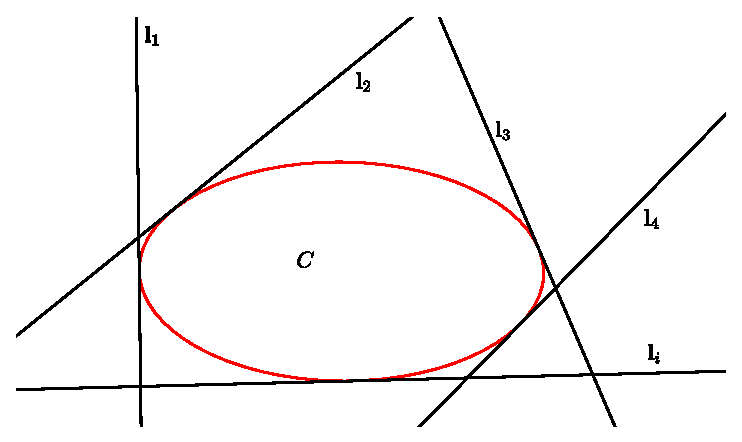
\includegraphics[width=\hsize]{conica-envelope}
\legend{A cônica $C$ é o envelope de todas as retas $\lightrgb_i$ que satisfazem $\lightrgb^\top C^*\,\lightrgb=0$.}
\source{O autor.}
\label{fig.conica-envelope}
\end{figure}
\subsection{Cônicas degeneradas}\label{sec.conicas-degeneradas}

Quando a matriz que representa a cônica não tem posto completo ocorrem cônicas degeneradas, daí a cônica será duas retas caso a matriz tenha posto $2$ ou uma reta repetida caso a matriz tenha posto $1$. Apresentamos a seguir dois exemplos de cônicas degeneradas, uma cônica ponto e uma cônica dual. A cônica 
\begin{equation*}
C=\lightrgb\,{\bf m}^\top+{\bf m}\,\lightrgb^\top
\end{equation*}
é uma cônica ponto composta por duas retas $\lightrgb$ e ${\bf m}$. Assim, se um ponto $\x\in\lightrgb$ então $\lightrgb^\top\x=0$ e esse ponto deve satisfazer $\x^\top C\,\x=0$. De fato,
\begin{equation*}
\begin{array}{rcl}
\x^\top C\,\x&=&\x^\top(\lightrgb\,{\bf m}^\top+{\bf m}\,\lightrgb^\top)\,\x\\
&=&\x^\top\lightrgb\,{\bf m}^\top\x+\x^\top {\bf m}\,\lightrgb^\top\x\\
&=&0\,{\bf m}^\top\x+\x^\top{\bf m}\,0\\
&=&0.
\end{array}
\end{equation*}
A argumentação é analoga caso $\x\in{\bf m}$. A equação de uma cônica dual degenerada é composta por pontos e a matriz correspondente tem posto 2 caso seja composta por dois pontos, ou posto 1 caso seja composta por um ponto repetido, 
\begin{equation*}
C^*=\x\,\y^\top+\y\,\x^\top.
\end{equation*}
De forma análoga à argumentação anterior podemos demosntrar que $C^*$ define um equação em retas,
\begin{equation*}
\lightrgb^\top\,C^*\lightrgb=0.
\end{equation*}
\subsection{A relação polo-polar}\label{sec.polo-polar}

Vimos anteriormente que uma reta $\lightrgb$ é tangente a uma cônica num ponto $\x$ se 
\begin{equation*}
\lightrgb=C\,\x.
\end{equation*}
Mas se o ponto $\x$ não pertence à cônica $C$ então temos uma relação denominada \textit{polo-polar}, onde a reta $\lightrgb$ é chamada reta \textit{polar} de $\x$, e $\x$ é chamado o \textit{polo} da reta $\lightrgb$, conforme a ilustração na Figura \ref{fig.polo-polar}.

A reta polar $\lightrgb=C\,\x$ intercepta a cônica 
$C$ em dois pontos $\y_1$ e $\y_2$, e as retas tangentes à cônica $C$ nesses dois pontos se interceptam em $\x$. De fato, considere o ponto $\y_1 \in C$ e a reta tangente a esse ponto ${\bf m}=C\,\y_1$. Essa tangente contém o ponto $\x$ se 
\begin{equation*}
\x^\top{\bf m}=0\qquad\text{ou}\qquad\x^\top C\,\y_1=0,
\end{equation*}  
e, usando a simetria da cônica $C$ e aplicando a transposição em $\x^\top C$, temos
\begin{equation*}
\x^\top C\,\y_1=(C\,\x)^\top\y_1=0,
\end{equation*}
mostrando que o ponto $\y_1$ pertence à reta $\lightrgb=C\,\x$. Assim, a reta $\lightrgb$ intercepta a cônica $C$ no ponto $\y_1$, no qual a tangente a $C$ contém o ponto $\x$. Observa-se que se o ponto $\x$ se aproxima da cônica $C$, os dois pontos $\y_1$ e $\y_2$ vão se aproximando um do outro, e quando ponto $\x$ pertence à conica $C$ a reta polar se torna a reta tangente. O argumento é análogo para $\y_2$.
\begin{figure}[!htb]{\textwidth}
\caption{Relaç\~ao polo-polar.}
\subfloat[]{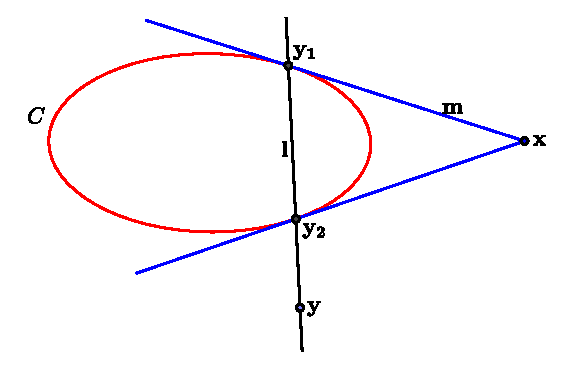
\includegraphics[width=.49\hsize]{polo-polar}}\hfill
\subfloat[]{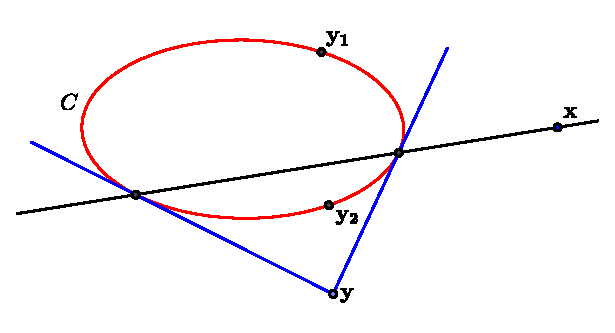
\includegraphics[width=.49\hsize]{polo-polar-simetria}}\hfill
\legend{(a) A reta $\lightrgb=C\,\x$ é a reta polar de $\x$, e o ponto $\x=C^{-1}\lightrgb$ é o polo da reta $\lightrgb$. Os pontos $\x$ e $\y$ são chamados conjugados, pois obedecem à relação $\y^\top C\,\x=0$. (b) Duplicação da figura para visualização da simetria da relação polo-polar. O ponto $\x$ pertence à reta polar de $\y$.}
\source{O autor.}
\label{fig.polo-polar}
\end{figure}\\

\noindent {\bf Pontos conjugados.}

Quando um ponto $\y$ qualquer pertence à reta polar $\lightrgb=C\,\x$ temos que 
\begin{equation*}
\y^\top\lightrgb=\y^\top C\,\x=0,
\end{equation*}
e quaisquer dois pontos que satisfazem a relação $\y^\top C\,\x=0$ são chamados \textit{conjugados} com relação à cônica $C$. Repare que o ponto $y$ não precisa necessariamente pertencer à cônica. Mais ainda, se um ponto $\y$ está na reta polar de $\x$, então $\x$ está na reta polar de $\y$. Como vimos, se $\y$ está na reta polar de $\x$ vale a relação $\y^\top C\,\x=0$, e tomando a transposta temos que $\x^\top C\,\y=0$, pois $C$ é simétrica. 
%Existe uma relacao de conjugacao para retas, digamos ${\bf l}$ e ${\bf m}$: ${\bf l}^\top C^*{\bf m}=0$.
\subsection{Transformações projetivas em $\mathbb{P}^2$}\label{sec.trans-proj-H}

A tranformação projetiva também conhecida como projetividade, colineação ou homografia,  é uma função (invertível) que leva pontos no plano $\mathbb{P}^2$ em pontos no plano $\mathbb{P}^2$ preservando a colinearidade desses pontos. Mais formalmente, uma função $h:\mathbb{P}^2\rightarrow\mathbb{P}^2$ é uma transformação projetiva se, e somente se, existe uma matriz $H_{3\times3}$ onde para cada ponto $\x\in\mathbb{P}^2$ temos que $h(\x)=H\,\x$ pertencente a $\x\in\mathbb{P}^2$. De fato, dados três pontos $\x_1$, $\x_2$ e $\x_3$ na mesma reta $\lightrgb$, temos que $\lightrgb^\top\x_i=0$ para $i=1,2 \,\,\,\text{e}\,\,\, 3$. Seja dada ainda uma matriz invertível $H_{3\times3}$. Definindo
\begin{equation*}
\lightrgb'=H^{-\top}\lightrgb \qquad\text{e}\qquad \x'_i=H\,\x_i,
\end{equation*}
vemos que todos os pontos $\x'_i$ pertencem à reta $\lightrgb'$, pois
\begin{equation*}
\begin{array}{rcl}
\lightrgb'^\top\x'_i&=&(H^{-\top}\lightrgb)^\top H\,\x_i\\
&=&\lightrgb^\top H^{-1}H\,\x_i\\
&=&\lightrgb^\top\x_i=0
\end{array}
\end{equation*}
preservando assim, a colinearidade dos pontos. A implicação direta é demasiadamente grande. A argumentação mostra que qualquer transformação linear aplicada a coordenadas homogêneas é uma transformação projetiva em $\mathbb{P}^2$, ou seja, a transformação projetiva é simplesmente uma transformação linear em $\mathbb{R}^3$. Podemos ver que o efeito da matriz $H$ não é alterado pela multiplicação por um escalar diferente de zero na equação
\begin{equation*}
\x'=H\,\x,
\end{equation*}
pois os pontos permanecem colineares após a transformação, alterando apenas a escala. Assim, a matriz $H$ é homogênea, e apenas a razão entre os seus elementos é significante, ou seja, são nove elementos mas oito graus de liberdade. Os pontos $\x\leftrightarrow\x'$ são chamados {\it pontos correspondentes}.\\

\noindent {\bf Transformação de retas.}

Na argumentação anterior vimos que a reta $\lightrgb'$ foi definida na forma $\lightrgb'=H^{-\top}\lightrgb$. Tal definição não foi em vão, pois a definição nesta forma garante que os pontos depois de transformados permaneçam colineares. Assim, a transformação projetiva de pontos nos dá essa regra para transformação projetiva de retas.\\

\noindent {\bf Transformação de cônicas.}

Invertendo a função $\x'=H\,\x$ temos que $\x=H^{-1}\x'$, e substituindo $\x$ na equação matricial de uma cônica $\x^\top C\,\x=0$ temos
\begin{equation*}
\begin{array}{rcl}
\x^\top C\,\x&=&(H^{-1}\x')^\top C\,H^{-1}\x'\\
&=&\x'^\top H^{-\top}C\,H^{-1}\x'\\
&=&\x'^\top C'\x'=0
\end{array}
\end{equation*}
onde $\x'^\top C'\x'=0$ é a equação matricial da cônica depois de aplicada a transformação projetiva, com $C'=H^{-\top}C\,H^{-1}$ sendo a regra para a transformação de cônicas.
\subsection{A geometria projetiva de uma dimensão}\label{sec.geometria-1D}
Vamos abrir um parênteses na discussão sobre o plano ${\mathbb{P}^2}$ para discorrer brevemente sobre a {\it reta projetiva} ${\mathbb{P}}$. A reta projetiva tem muita similaridade com o plano projetivo, pois pontos na reta são representados em coordenadas homogêneas (vetores com duas componentes) e são projetivamente transformados de acordo com uma homografia $H_{2\times2}$. Na reta projetiva ${\mathbb{P}}$ os pontos têm as seguintes notação e transformação projetiva: 
\begin{equation}\label{eq.ponto-homografia-em-P}
\overline{\x}=
\begin{pmatrix}
x_1\\
x_2
\end{pmatrix}
\qquad\text{e}\qquad
\overline{\x}'=H\,\overline{\x}.
\end{equation}
Pontos no infinito têm a componente $x_2=0$.
\begin{figure}[!htb]{\textwidth}
\caption{Razão cruzada.}
\subfloat[]{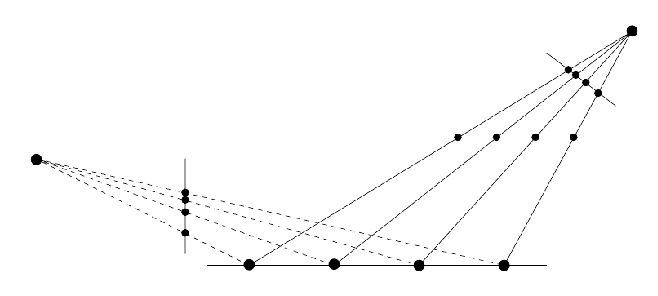
\includegraphics[width=.6\hsize]{geometria-P1}}\hfill
\subfloat[]{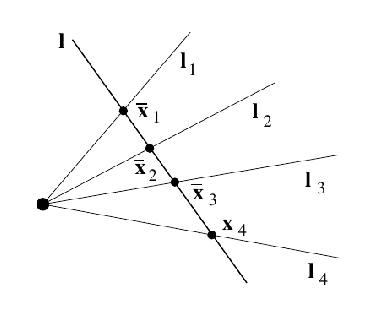
\includegraphics[width=.3\hsize]{razao-cruzada-retas}}\hfill
\legend{$({\tt a})\,$Cada grupo de quatro pontos está relacionado aos outros grupos por uma transformação projetiva em ${\mathbb{P}}$. Como a razão cruzada é uma invariante, tais grupos possuem a mesma razão cruzada. $\,({\tt b})\,$A razão cruzada das quatro retas é uma invariante projetiva do plano que as contém (ver Subseção \ref{sec.hierarquia-transformacoes}). As retas contendo os quatro pontos podem ser vistas em ${\mathbb{P}^2}$ como planos de imagens, objetos planares, relacionados por centros de projeção.}
\source{Hartley e Zisserman (2004).}
\label{fig.razao-cruzada}
\end{figure}
\section*{A razão cruzada.}
A definição a seguir é uma \textit{invariante} (ver Subseção \ref{sec.hierarquia-transformacoes}) básica da geometria projetiva. Dados quatro pontos numa reta, conforme a Figura \ref{fig.razao-cruzada}, a razão cruzada é definida por 
\begin{equation*}
\text{cross}(\overline{\x}_1,\overline{\x}_2,\overline{\x}_3,\overline{\x}_4)=\frac{|\overline{\x}_1\,\overline{\x}_2||\overline{\x}_3\,\overline{\x}_4|}{|\overline{\x}_1\,\overline{\x}_3||\overline{\x}_2\,\overline{\x}_4|},
\end{equation*}
onde 
\begin{equation*}
|\overline{\x}_i\,\overline{\x}_j|=
\text{det}
\begin{bmatrix}
x_{i1}&x_{j1}\\
x_{i2}&x_{j2}
\end{bmatrix}.
\end{equation*}
Vamos verificar que a razão cruzada é uma invariante sob transformação projetiva, ou seja, dada uma homografia como a Equação \ref{eq.ponto-homografia-em-P} temos que 
\begin{equation}\label{eq.invariante-cross}
\text{cross}(\overline{\x}'_1,\overline{\x}'_2,\overline{\x}'_3,\overline{\x}'_4)=\text{cross}(\overline{\x}_1,\overline{\x}_2,\overline{\x}_3,\overline{\x}_4).
\end{equation}
De fato,
\begin{equation*}
\begin{array}{rcll}
\text{cross}(\overline{\x}'_1,\overline{\x}'_2,\overline{\x}'_3,\overline{\x}'_4)&=&\displaystyle\frac{|\overline{\x}'_1\,\overline{\x}'_2||\overline{\x}'_3\,\overline{\x}'_4|}{|\overline{\x}'_1\,\overline{\x}'_3||\overline{\x}'_2\,\overline{\x}'_4|}&\text{como}\qquad\overline{\x}'=H\,\overline{\x}\\\\
&=&
\displaystyle\frac{|H\,\overline{\x}_1\,H\,\overline{\x}_2||H\,\overline{\x}_3\,H\,\overline{\x}_4|}{|H\,\overline{\x}_1\,H\,\overline{\x}_3||H\,\overline{\x}_2\,H\,\overline{\x}_4|}&\\\\
&=&
\displaystyle\frac{|H\,[\overline{\x}_1\,\overline{\x}_2]||H\,[\overline{\x}_3\,\overline{\x}_4]|}{|H\,[\overline{\x}_1\,\overline{\x}_3]||H\,[\overline{\x}_2\,\overline{\x}_4|]}&[\overline{\x}_i\,\overline{\x}_j]\quad\text{é matriz}      \\\\
&=&
\displaystyle\frac{|H|\,|\overline{\x}_1\,\overline{\x}_2|\,|H|\,|\overline{\x}_3\,\overline{\x}_4|}{|H|\,|\overline{\x}_1\,\overline{\x}_3|\,|H|\,|\overline{\x}_2\,\overline{\x}_4|}&\\\\
&=&
\displaystyle\frac{|\overline{\x}_1\,\overline{\x}_2||\overline{\x}_3\,\overline{\x}_4|}{|\overline{\x}_1\,\overline{\x}_3||\overline{\x}_2\,\overline{\x}_4|}&\\\\
&=&
\text{cross}(\overline{\x}_1,\overline{\x}_2,\overline{\x}_3,\overline{\x}_4),
\end{array}
\end{equation*}
e portanto a Equação \ref{eq.invariante-cross} segue.

Como corolário, segundo Semple e Kneebone (1952), existe homografia $H$ onde $\overline{\x}'_i=H\,\overline{\x}_i$ se, e somente se, $\text{cross}(\overline{\x}_1,\overline{\x}_2,\overline{\x}_3,\overline{\x}_4)=\text{cross}(\overline{\x}'_1,\overline{\x}'_2,\overline{\x}'_3,\overline{\x}'_4)$. 

%Como a implicação direta já foi feita na argumentação anterior, vamos fazer a implicação contrária. Sabemos que a razão cruzada é invariante sob projetividade, portanto
%
%\begin{equation*}
%\text{cross}(\overline{\x}_1,\overline{\x}_2,\overline{\x}_3,\overline{\x}_4)=\text{cross}(H\,\overline{\x}_1,H\,\overline{\x}_2,H\,\overline{\x}_3,H\,\overline{\x}_4).
%\end{equation*}
%Como
%
%\begin{equation*}
%\text{cross}(\overline{\x}_1,\overline{\x}_2,\overline{\x}_3,\overline{\x}_4)=\text{cross}(\overline{\x}'_1,\overline{\x}'_2,\overline{\x}'_3,\overline{\x}'_4),
%\end{equation*}
%temos que
%
%\begin{equation*}
%\text{cross}(\overline{\x}'_1,\overline{\x}'_2,\overline{\x}'_3,\overline{\x}'_4)=\text{cross}(H\,\overline{\x}_1,H\,\overline{\x}_2,H\,\overline{\x}_3,H\,\overline{\x}_4).
%\end{equation*}
%Assim,
%
%\begin{equation*}
%\overline{\x}'=H\,\overline{\x}.
%\end{equation*}
\section*{Retas concorrentes.}
Vimos que pontos e retas têm representações similares em ${\mathbb{P}^2}$ usando vetores homogêneos com três componentes. Daí, fazendo as devidas alterações, todo teorema relacionado a pontos são válidos também para retas, e dizemos que existe a {\it dualidade} entre pontos e retas no plano ${\mathbb{P}^2}$. Analogamente,  
quatro retas concorrentes em um único ponto têm geometria em ${\mathbb{P}}$ dual com quatro pontos colineares, assim a razão cruzada entre essas retas também é uma invariante sob projetividade. Conforme a Figura \ref{fig.razao-cruzada}, o valor da razão cruzada entre as quatro retas é dado pelos pontos de interseção de uma quinta reta transversal a essas quatro, ou seja
\begin{equation*}
\text{cross}(\lightrgb_1,\lightrgb_2,\lightrgb_3,\lightrgb_4)=\text{cross}(\overline{\x}_1,\overline{\x}_2,\overline{\x}_3,\overline{\x}_4).
\end{equation*}
Tal asserção é devida ao teorema de \textit{Pappus} conforme Springer (1964). 
\subsection{Subgrupo de transformações projetivas}\label{sec.hierarquia-transformacoes}
As transformações projetivas se dividem em subgrupos de transformações com características mais específicas. Esses subgrupos são as \textit{isometrias}, \textit{similaridades}, \textit{afinidades} e a própria \textit{transformação projetiva}. Cada subgrupo mantém \textit{invariante} algumas propriedades do objeto ao qual a transformação está sendo aplicada. Por exemplo, a distância entre dois pontos num quadrado se mantém a mesma após a aplicação de uma transformação isométrica (translação, rotação e possível reflexão), mas pode variar após a aplicação de uma transformação de similaridade, a qual pode gerar um quadrado maior ou menor que o original. Portanto, distância entre dois pontos é uma invariante sob isometria mas não é sob similaridade.
\section*{Transformação isométrica.}
É representada pela matriz
\begin{equation*}
\begin{bmatrix}
\epsilon\,cos\,\theta&-sen\,\theta&t_x\\
\epsilon\,sen\,\theta&cos\,\theta&t_y\\
0&0&1
\end{bmatrix},
\end{equation*}
onde $\epsilon=\pm1$. Se $\epsilon=1$ a isometria preserva a orientação e é chamada \textit{Transformação Euclidiana} (composição de translação e rotação). Se $\epsilon=-1$ a isometria reverte a orientação. A transformação Euclidiana é o tipo de isometria mais importante, denotada por $H_E$ e representada pela matriz em forma de blocos
\begin{equation*}
H_E=
\begin{bmatrix}
R&{\bf t}\\
{\bf 0}^\top&1
\end{bmatrix}.
\end{equation*}
Sendo $R_{2\times2}$ uma matriz de rotação, ${\bf t}$ um vetor com duas componentes e ${\bf 0}=(0,0)^\top$ um vetor nulo, essa transformação tem três graus de liberdade, um para o ângulo de rotação em $R$ e dois para o vetor de translação. Assim, são necessários no mínimo dois pontos correspondentes $\x_i\leftrightarrow\x'_i$ para determinarmos a matriz da transformação Euclidiana. As invariantes são distância entre dois pontos, ângulo entre duas retas e área. 
\section*{Tranformação de similaridade.}
A transformação de similaridade é denotada por $H_S$ e é representada pela matriz 
\begin{equation*}
H_S=
\begin{bmatrix}
s\,cos\,\theta&-s\,sen\,\theta&t_x\\
s\,sen\,\theta&s\,cos\,\theta&t_y\\
0&0&1
\end{bmatrix},
\end{equation*} 
que neste caso é a composição de uma transformação Euclidiana com uma escala (sem reflexão) $s$. A transformação de similaridade preserva a forma dos objetos e tem quatro graus de liberdade, com o escalar $s$ contando para um grau a mais que a transformação Euclidiana. A similaridade também pode ser determinada usando dois pontos correspondentes e tem a matriz em bloco
\begin{equation*}
H_S=
\begin{bmatrix}
s\,R&{\bf t}\\
\,{\bf 0}^\top&1
\end{bmatrix}.
\end{equation*}
Com a mudança na escala das figuras, a área e a distância entre dois pontos não é mais a mesma após a transformação, mas os ângulos entre as retas não mudam, e pontanto, ângulo é uma invariante sob similaridade. Em particular, retas paralelas permanecem paralelas. A razão entre as distâncias antes e após a transformação permanece a mesma por conta do cancelamento da escala, e analogamente, a razão entre as áreas também permanece a mesma.
\section*{Transformação afim.}
A transformação afim, ou afinidade, é uma transformação linear seguida de uma translação, denotada por $H_A$ e representada pela matriz
\begin{figure}[!htb]{\textwidth}
\caption{Transformação afim.}
\subfloat[]{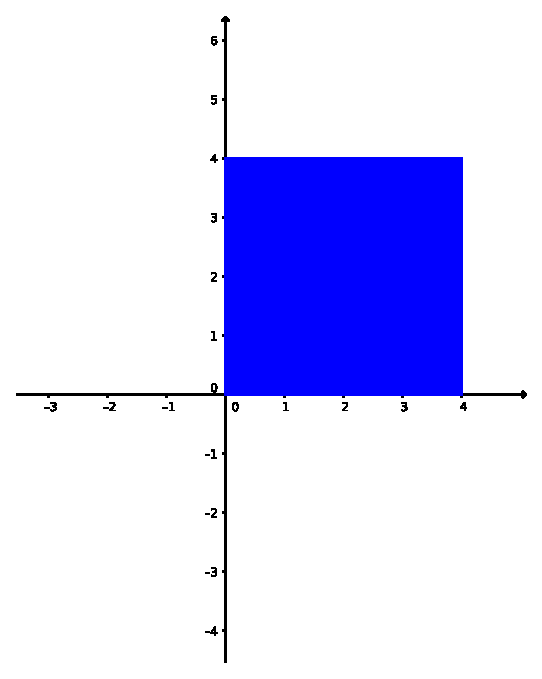
\includegraphics[width=.19\hsize]{quadrado-1}}
\,
\subfloat[]{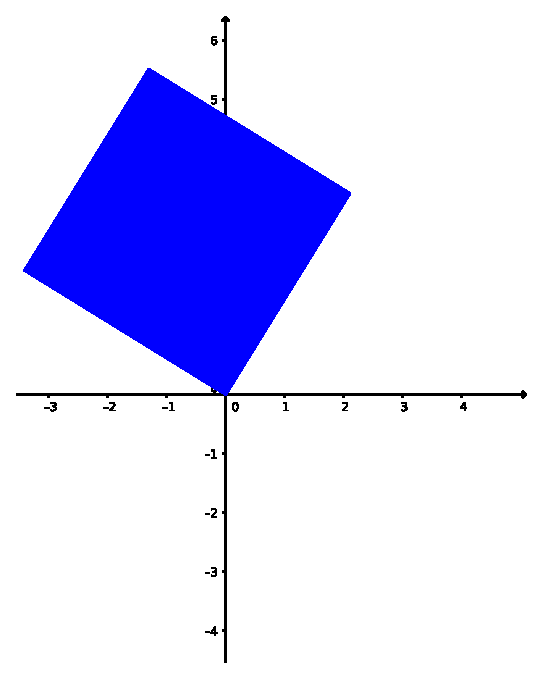
\includegraphics[width=.19\hsize]{quadrado-2}}
\,
\subfloat[]{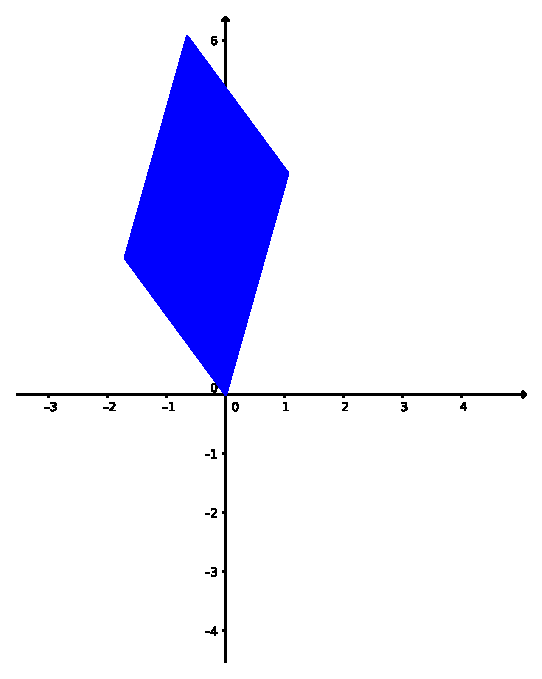
\includegraphics[width=.19\hsize]{losango-1}}
\,
\subfloat[]{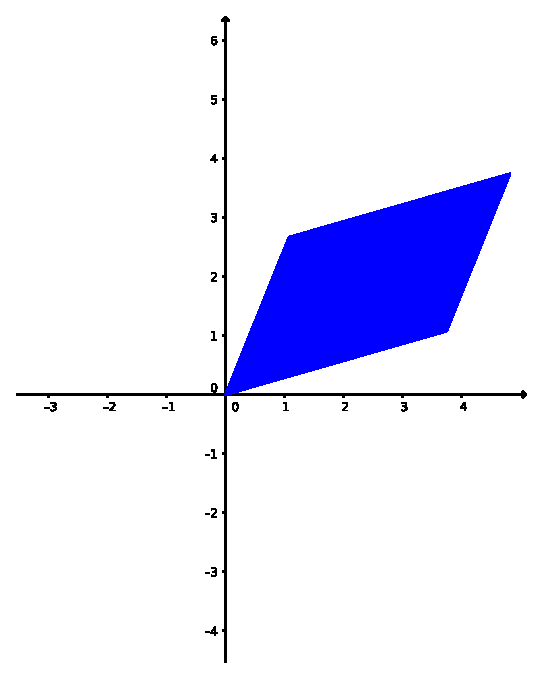
\includegraphics[width=.19\hsize]{losango-2}}
\,
\subfloat[]{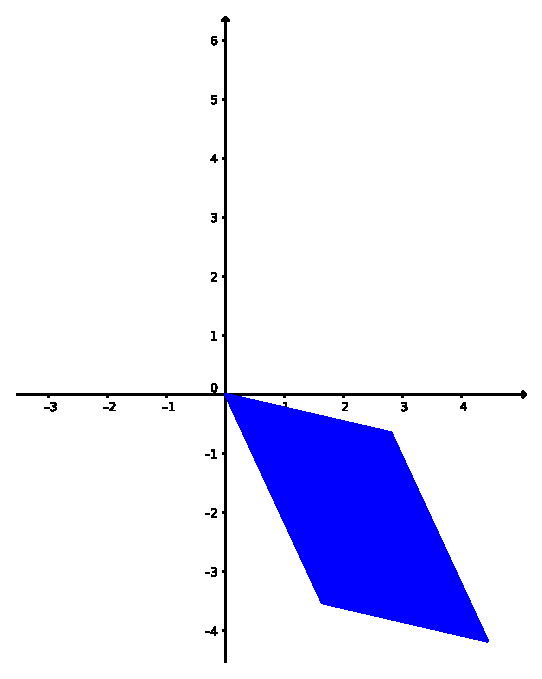
\includegraphics[width=.19\hsize]{losango-3}}
\legend{$({\tt a})\,$Um quadrado.$\,({\tt b})\,$Rotação $R(50^\circ)$.$\,({\tt c})\,$Escala não uniforme $D$ com $\lambda_1=0,5$ e $\lambda_2=1,1$.$\,({\tt d})\,$Rotação $R(-50^\circ)$.$\,({\tt e})\,$Rotação final $R(-70^\circ)$.}
\source{O autor.}
\label{fig.angulos-afinidades}
\end{figure}
\begin{equation*}
H_A=
\begin{bmatrix}
a_{11}&a_{12}&t_x\\
a_{21}&a_{22}&t_y\\
0&0&1
\end{bmatrix}.
\end{equation*}
A matriz possui seis graus de liberdade correspondentes ao seis elementos da matriz, e são necessários três pontos correspondentes para determinarmos a matriz de afinidade que pode ser escrita em blocos como
\begin{equation*}
H_A=
\begin{bmatrix}
A&{\bf t}\\
{\bf 0}^\top&1
\end{bmatrix}.
\end{equation*}
Como uma forma de ajudar a entender os efeitos da matriz $A$ vamos decompô-la em transformações mais fundamentais
\begin{equation*}
A=R(\theta)R(-\phi)DR(\phi),
\end{equation*}
com uma matriz diagonal $D=diag(\lambda_1, \lambda_2)$ onde as componentes são escalares não-isotrópicos 
%\footnote{Isotrópico: É o que se diz de um corpo que, em todas as direções, apresenta as mesmas propriedades ópticas.} 
que alteram a escala nos eixos $x$ e $y$ respectivamente. Uma rotação $\phi$ que define o sentido de aplicação dos escalares da matriz $D$, uma rotação contrária $-\phi$ e uma última rotação $\theta$. Podemos visualizar os efeitos das rotações e dos escalares na Figura \ref{fig.angulos-afinidades}. Os dois graus de liberdade a mais em relação a uma similaridade vêm do ângulo $\phi$ e da razão entre os escalares aplicados por $D$, $\frac{\lambda_1}{\lambda_2}$. 


Temos três importantes invariantes sob afinidade: retas paralelas se matêm paralelas, razão entre seguimentos de retas paralelas e razão entre as áreas. Mesmo que retas paralelas sejam invariantes, a afinidade não mantém, em geral, o ângulo entre retas nem a razão entre as distâncias correspondentes como acontece com a similaridade.
\section*{Transformações projetivas.}
É uma transformação linear mais geral de coordenadas homogêneas (já definida na Subseção \ref{sec.trans-proj-H}), pois generaliza  a transformação de afinidade. Na forma de blocos temos a representação
\begin{equation*}
H_P=
\begin{bmatrix}
A&{\bf t}\\
{\bf v}^\top&v
\end{bmatrix},
\end{equation*}
onde ${\bf v}=(v_1,v_2)$. Como a matriz é $3\times3$ temos nove variáveis a serem determinadas, mas que se reduzem a oito tomando uma das variáveis para escala. Assim, precisamos de quatro pontos correspondentes para determinarmos os oito parâmetros da matriz. Além de manter a colinearidade dos pontos, uma invariante fundamental na transformação projetiva é a razão cruzada entre quatro pontos colineares, ou seja, a razão das razões de segmentos contidos numa mesma reta. Na Figura \ref{fig.transformacoes-2D} podemos ver um resumo das características geométricas preservadas (em um quadrado, por exemplo) por cada subgrupo de transformação.
\begin{figure}[!htb]{\textwidth}
\caption{Subgrupo de transformações projetivas.}
\subfloat{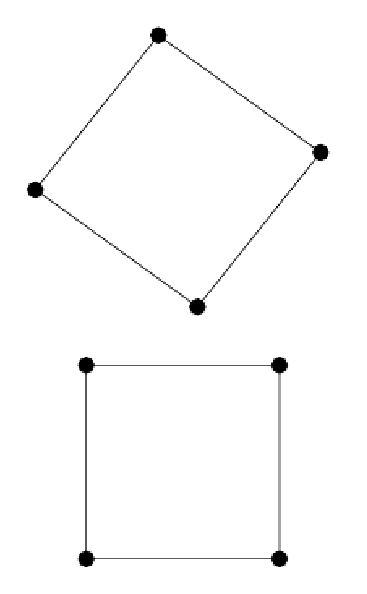
\includegraphics[width=.24\hsize]{trans-euclidiana-2D}}\hfill
\subfloat{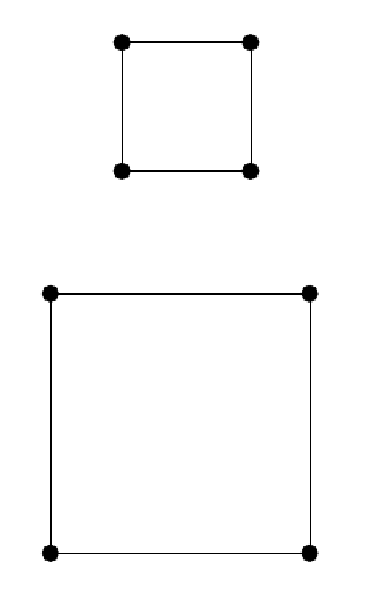
\includegraphics[width=.24\hsize]{trans-similaridade-2D}}\hfill
\subfloat{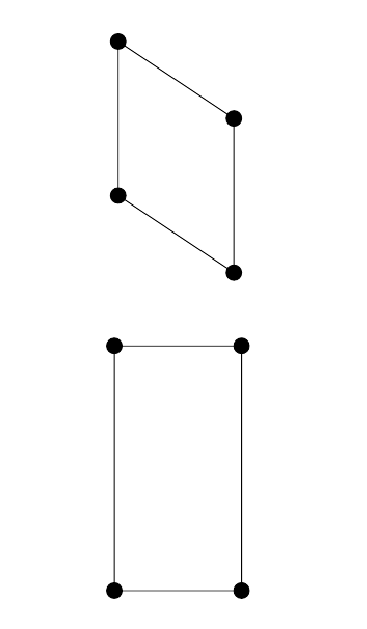
\includegraphics[width=.24\hsize]{trans-afinidade-2D}}\hfill
\subfloat{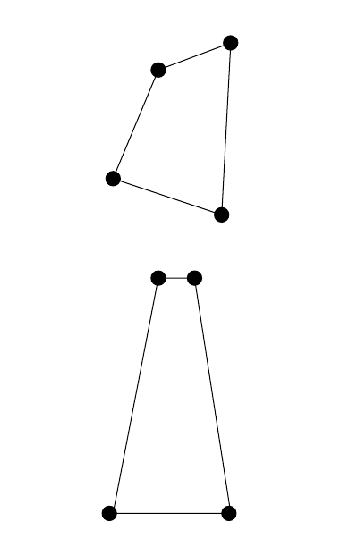
\includegraphics[width=.24\hsize]{trans-projetividade-2D}}\hfill
\legend{Respectivamente, transformações: euclidiana, similaridade, afinidade, e projetividade.}
\source{Adaptado, Hartley e Zisserman (2004).}
\label{fig.transformacoes-2D}
\end{figure}
\section{O espaço projetivo em três dimensões}\label{sec.espaco-P3}


\section*{O ponto.} 


Analogamente à representação de um ponto no plano $\mathbb{P}^2$, um ponto no espaço $\mathbb{P}^3$ é repesentado através de coordenadas homogêneas, acrescentando-se uma quarta coordenada ao vetor que representa esse ponto. Desta forma, $\X = (X_1,X_2,X_3,X_4)^\top$ e $X_4 \ne 0$, onde $\X$ é a representação em coordenadas homogêneas do ponto $(X,Y,Z)^\top \in \mathbb{R}^3$, e portanto um ponto nesse espaço tem três graus de liberdade. Para realizar tal mudança basta tomar 
\begin{equation*}
X=X_1/X_4 \,\, ,\, Y=X_2/X_4 \,\,\, \text{e} \,\,\, Z=X_3/X_4.
\end{equation*}
\section*{O plano.}

Temos que a representação algébrica de um plano $\bpi$ no espaço $\mathbb{R}^3$ é dada pela equação
\begin{equation*}
\pi_1\,X+\pi_2\,Y+\pi_3\,Z+\pi_4=0,
\end{equation*}
onde $\pi_i$ são os coeficientes da equação. Um ponto em $\mathbb{R}^3$ pertence ao plano se, e somente se, satifaz a equação acima que na forma matricial, usando a representação do ponto em coordenadas homogêneas, \'e dada por
\begin{equation*}
  (\pi_1,\pi_2,\pi_3,\pi_4)^\top
 \begin{pmatrix}
  X\\
  Y\\
  Z\\
  1
  \end{pmatrix}
 = 0.
\end{equation*}
Fazendo as substituições 
\begin{equation*}
X=X_1/X_4 \,\, , \,\, Y=X_2/X_4 \,\,\,\, \text{e} \,\,\,\, Z=X_3/X_4 ,
\end{equation*}

generalizamos a representação do ponto e a equação se torna
\begin{equation*}
\begin{array}{ccc}
(\pi_1,\pi_2,\pi_3,\pi_4)^\top
  \begin{pmatrix}
  X_1\\
  X_2\\
  X_3\\
  X_4
  \end{pmatrix}
  = 0
& \qquad \text{ou} \qquad
& \bpi^\top \, \X = 0.
\end{array}
\end{equation*}
Desta forma, verificamos que, assim como os pontos, um plano $\bpi = (\pi_1,\pi_2,\pi_3,\pi_4)^\top$ fica inteiramente determinado por um vetor com quatro coordenadas em $\mathbb{P}^3$. Aqui temos uma analogia com o espaço $\mathbb{P}^2$, já que pontos e retas têm a mesma representação vetorial com três componentes naquele espaço, e a dualidade entre pontos e retas em $\mathbb{P}^2$ também se verifica entre pontos e planos em $\mathbb{P}^3$. Como multiplicar a equação algébrica de um plano por um escalar diferente de zero não altera o plano, temos que os planos possuem três graus de liberdade. Podemos dividir as três primeiras coordenadas pela última, por exemplo, e fixar uma escala.

Obs: As três primeiras coordenadas do vetor que representa o plano corresponde ao vetor normal ao plano, conforme definido em Álgebra Linear.
\section*{A reta.}

Uma reta pode ser definida passando por dois pontos. Em $\mathbb{P}^2$, como os dois pontos estão no mesmo plano, uma reta passando por esses dois pontos tem apenas dois graus de liberdade, conforme visto anteriormente. Mas em $\mathbb{P}^3$, como os dois pontos podem estar em planos diferentes, temos que uma reta apresenta quatro graus de liberdade, dois graus para cada ponto. Assim, uma reta deveria ser representada por um vetor com cinco coordenadas em $\mathbb{P}^3$, mas vetores desse tipo não podem ser usados, facilmente, em expressões matemáticas que envolvem vetores com quatro coordenadas representando pontos e planos. Portanto é necessário encontrar uma outra representação, e uma das formas mais simples, de uso corrente em algoritmos, é definir a reta através de dois pontos não coincidentes (\cite{bib:kuang}). Outras representações de uma reta no espaço projetivo $\mathbb{P}^3$, diferentes da apresentada aqui, podem ser encontradas em \cite{Hartley2004}.


Uma reta ${\bf L}$ passando por dois pontos ${\bf A} \,\,\, \text{e} \,\,\, {\bf B}$ é representada pelo espaço linha gerado pela matriz $W$ composta pelos pontos ${\bf A}^\top \,\,\,\text{e} \,\,\, {\bf B}^\top$ em linha,
\begin{center}
$
\begin{array}{cc}
W = 
& \begin{bmatrix}
  A^\top\\
  B^\top
  \end{bmatrix},
\end{array}
$
\end{center}
onde o espaço gerado por $W^\top$ é o conjunto de pontos do tipo $a\,{\bf A} + b\,{\bf B}$ pertencentes à reta ${\bf L}$ procurada.
\section*{A quádrica.}


Similarmente à cônica em $\mathbb{P}^2$, uma quádrica $Q$ em $\mathbb{P}^3$ é definida pela equação
\begin{equation*}
\X^\top\,Q\,\X = 0,
\end{equation*}
onde $Q$ é uma matriz simétrica $4\times4$ com nove graus de liberdade.

\begin{figure}[!htb]{\textwidth}
\caption{Exemplos de qu\'adricas.}
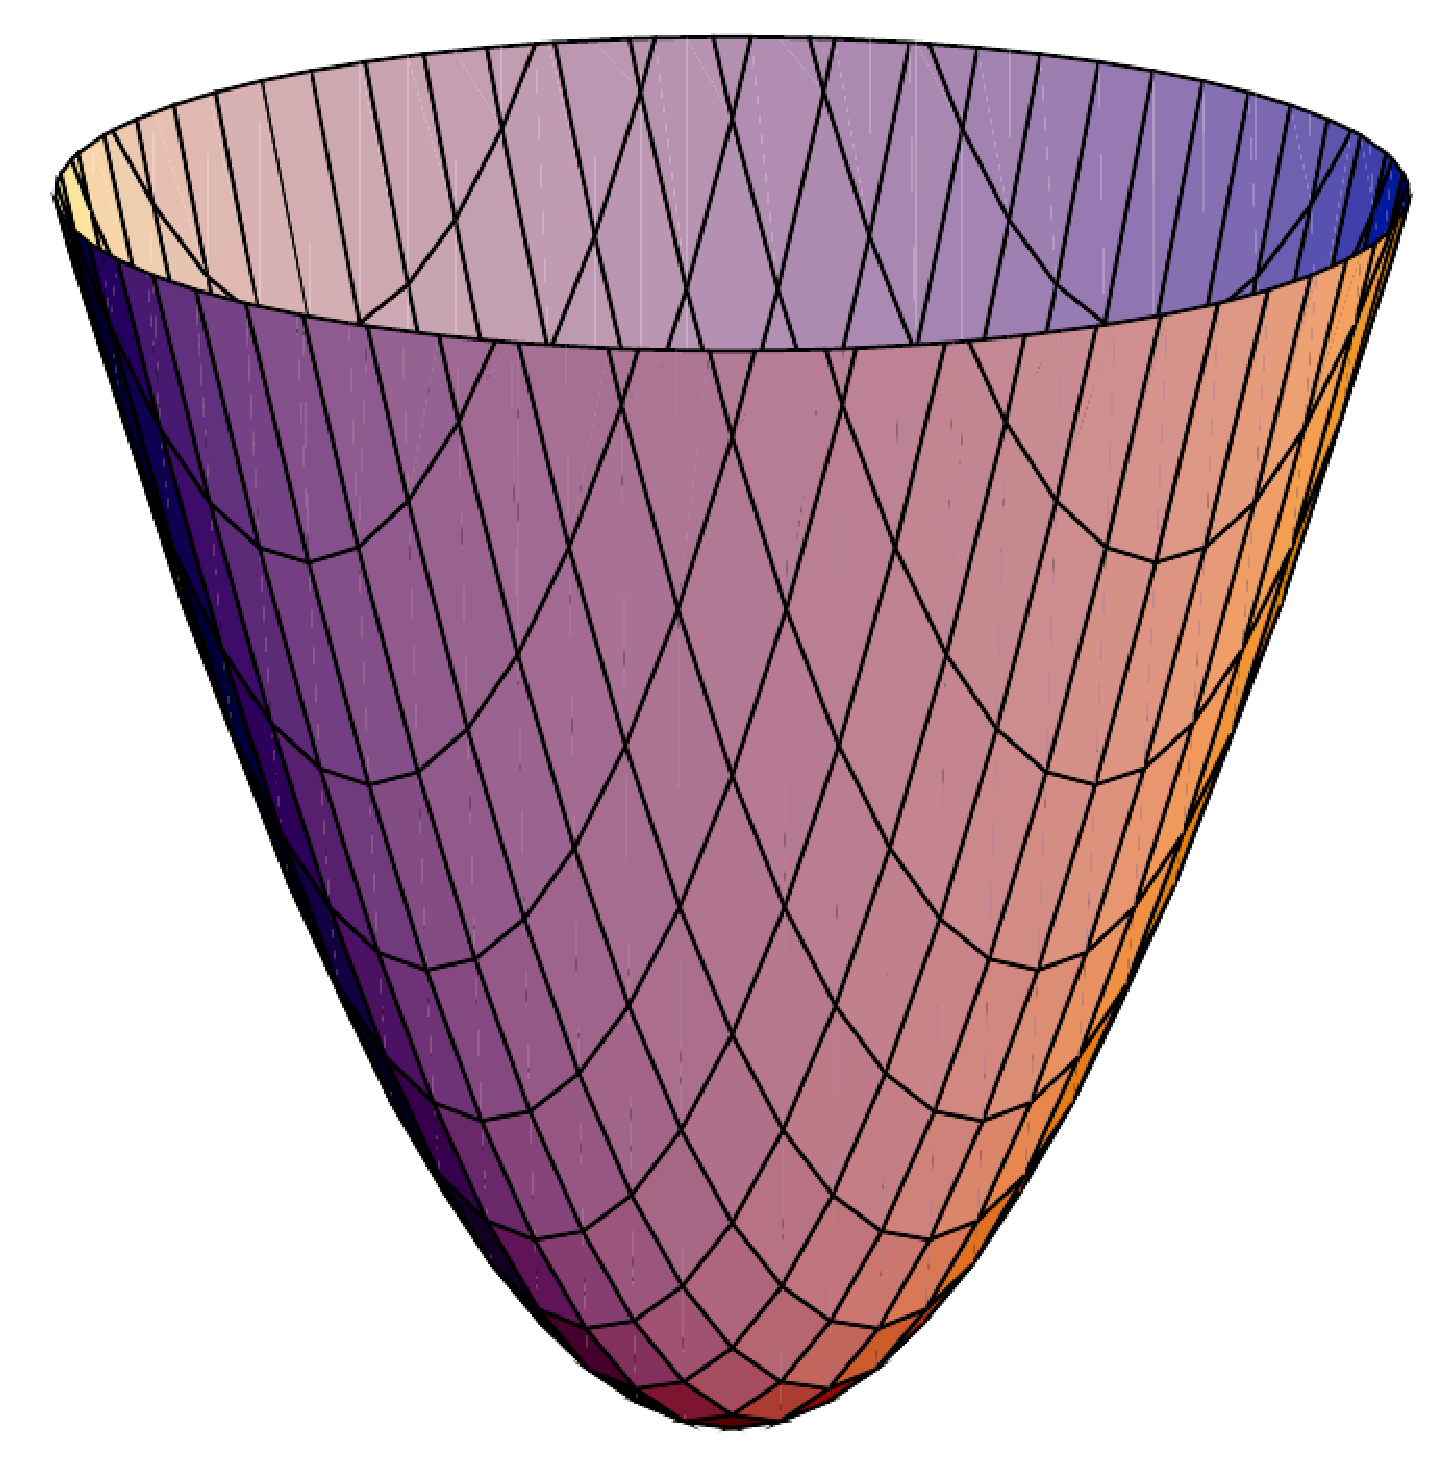
\includegraphics[width=.5\hsize]{paraboloide}\hfill
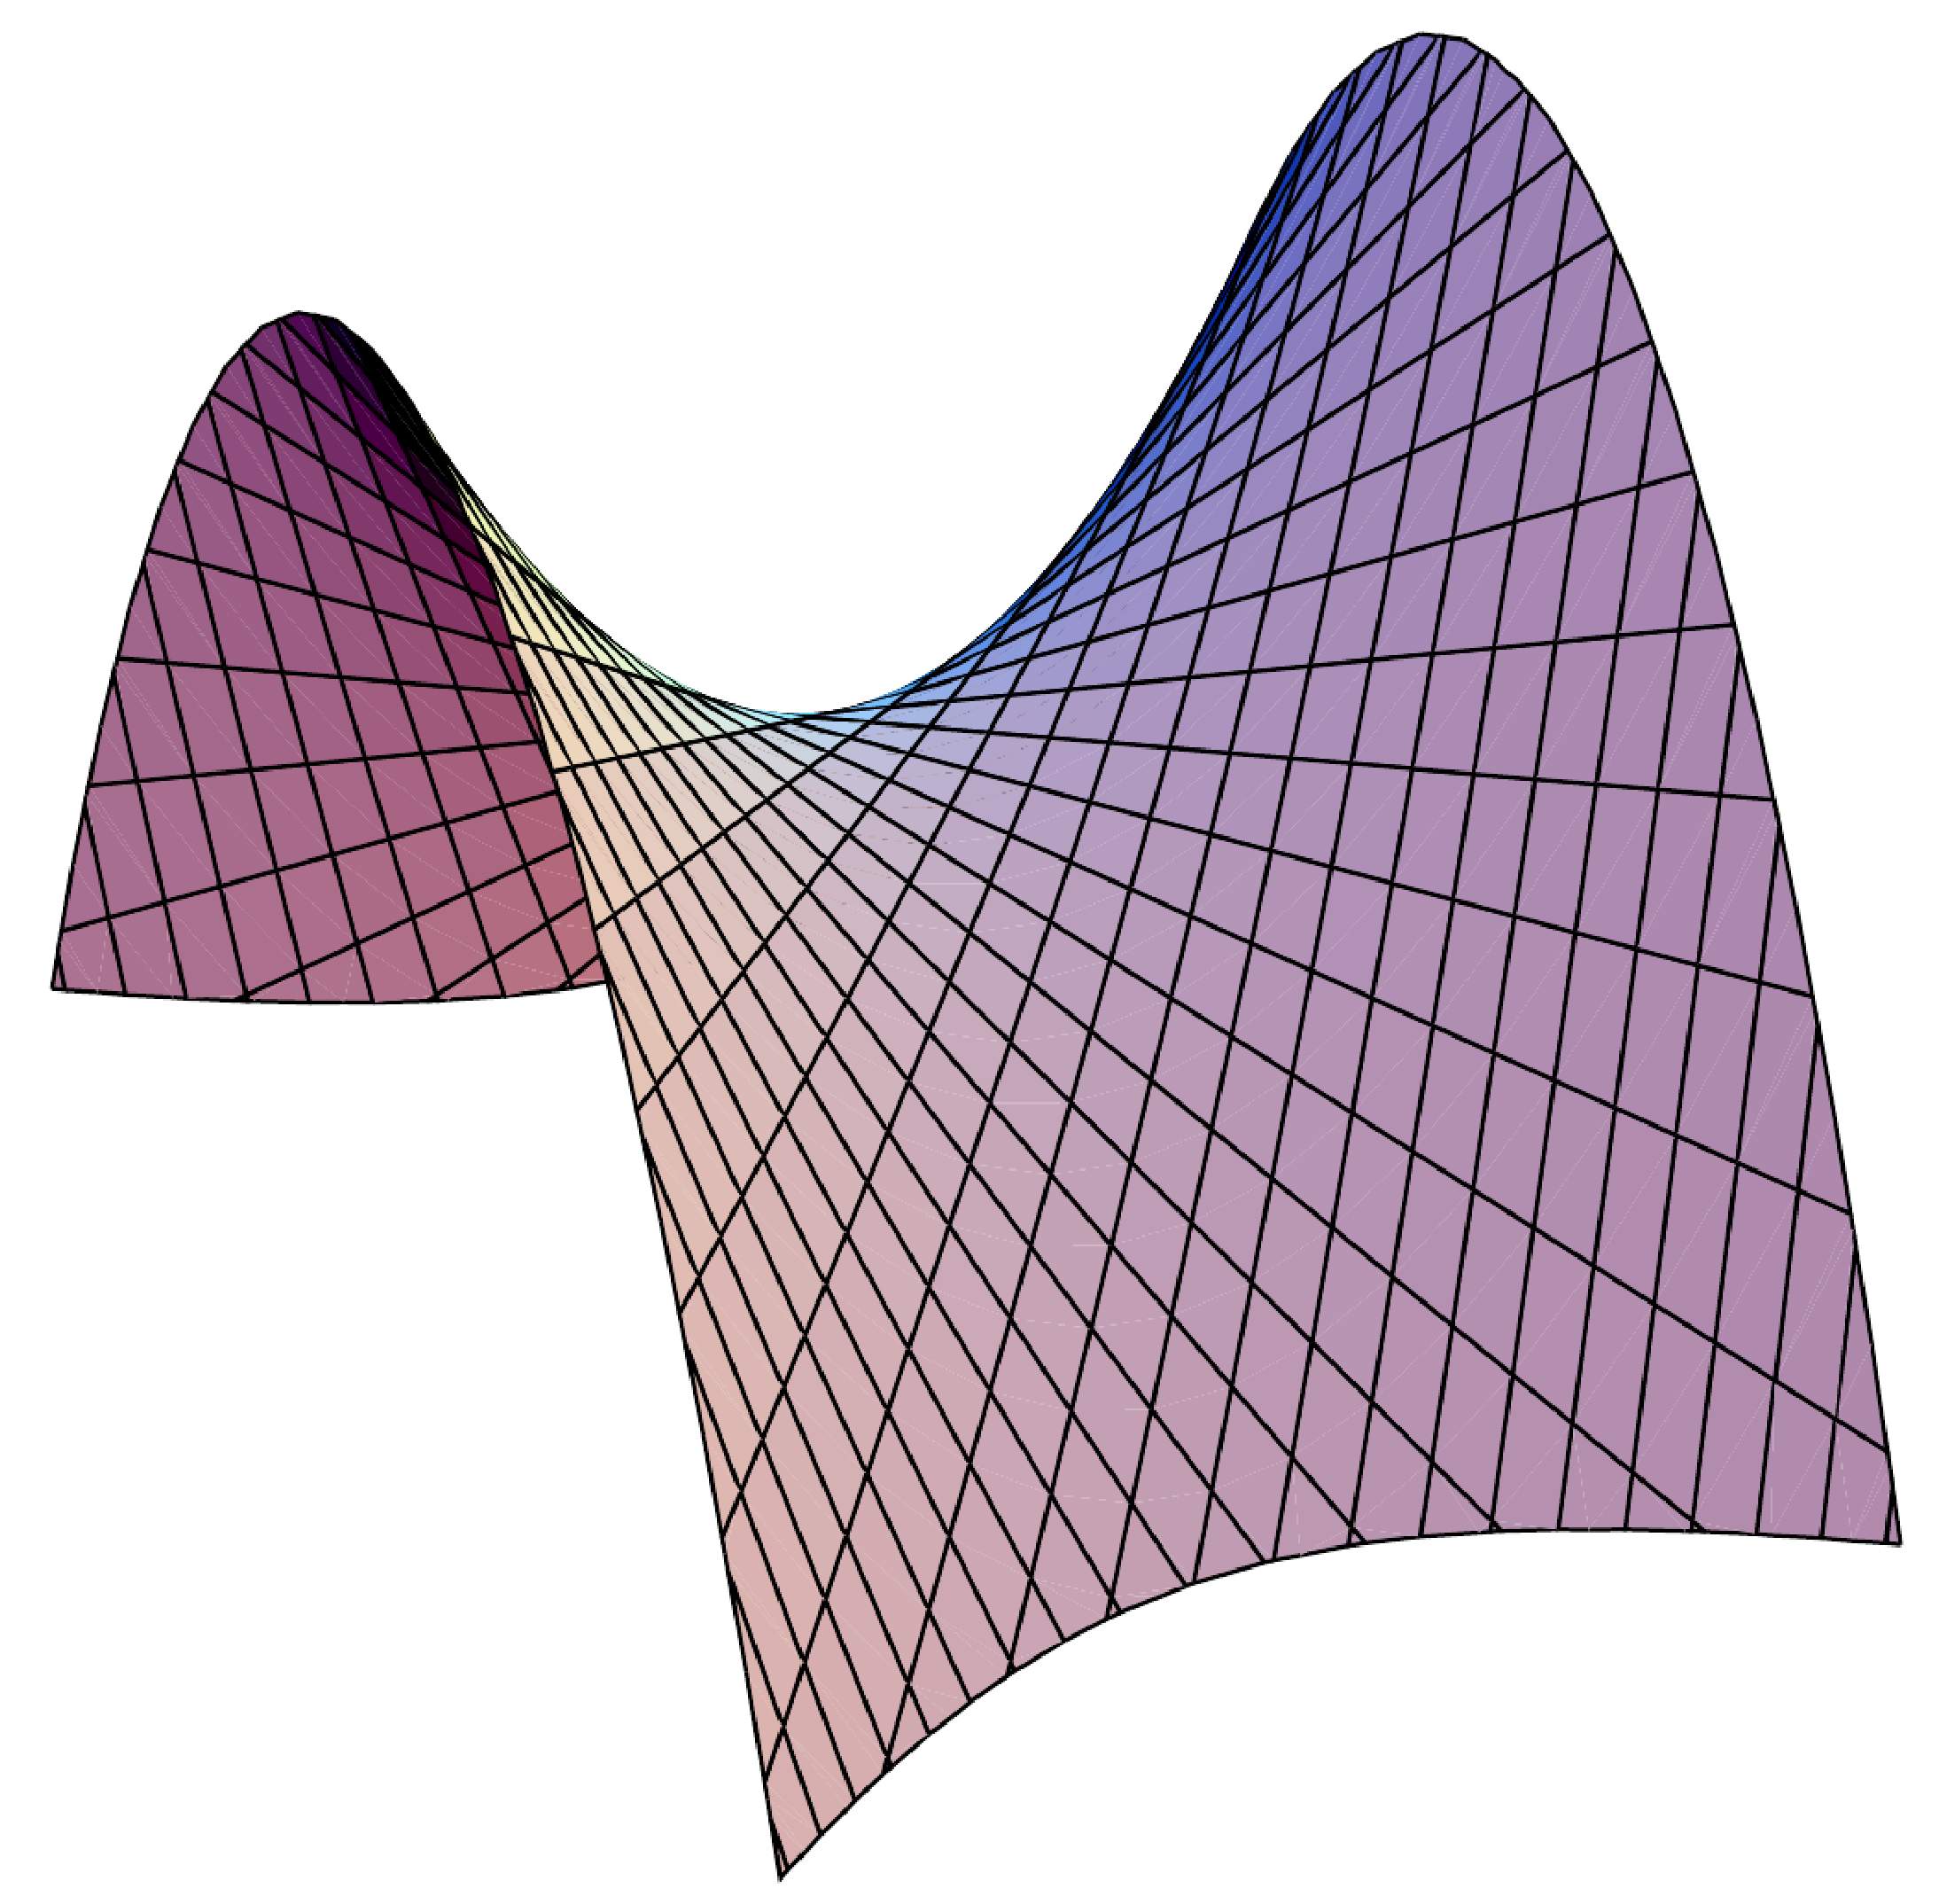
\includegraphics[width=.48\hsize]{hiperboloide_1_folha}\hfill
\legend{Parabolóide à esquerda e hiperbolóide de uma folha à direita.}
\source{Hartley e Zisserman (2004).}
\label{quadricas2}
\end{figure}
Mais detalhes sobre a dedução da definição de uma quádrica podem ser encontrados em Hartley e Zisserman (2004), bem como outros exemplos além daqueles observados na Figura \ref{quadricas2}.\\
\subsection{A transformação de pontos e planos em $\mathbb{P}^3$}\label{sec.trans-pontos-planos-P3}

A transformação de pontos e planos em $\mathbb{P}^3$ é inteiramente análoga àquela argumentada na Subseção \ref{sec.trans-proj-H} para pontos e retas em $\mathbb{P}^2$, pois assim como os pontos têm uma relação dual com retas em $\mathbb{P}^2$, os pontos também têm uma relação dual com planos em $\mathbb{P}^3$ e, como vimos, ambos têm a mesma representação em vetores homogêneos com quatro componentes. Assim, sob uma tranformação projetiva de pontos $\X'=H_{4\times4}\X$ temos que planos se transformam de acordo com:
\begin{equation*}
\bpi'=H^{-\top}\bpi.
\end{equation*}
\subsection{Direções e o plano no infinito.}\label{sec.direcoes-plano-infinito}

O plano no infinito é denotado por $\bpi_\infty$, tem a forma canônica $\bpi_\infty=(0,0,0,1)^\top$ e é composto por pontos no infinito $D=(X_1,X_2,X_3,0)^\top$ que são as direções das retas contidas no espaço. No plano projetivo $\mathbb{P}^2$ duas retas paralelas se encontram num ponto no infinito, e analogamente, em  $\mathbb{P}^3$ dois planos paralelos se encontram numa reta que está contida no plano no infinito, e também, uma reta é paralela a outra reta (ou a um plano) se o ponto de interseção está no $\bpi_\infty$. O plano no infinito é invariável sob uma transformação afim.

De acordo com a Subseção \ref{sec.trans-pontos-planos-P3} temos que a transformação projetiva de planos no espaço  $\mathbb{P}^3$ se dá pela fórmula $\bpi'=H^{-\top}\bpi$, assim podemos verificar porque um plano no infinito é invariante sob a tranformação afim. Conforme a Subseção \ref{sec.hierarquia-transformacoes} vimos que a transformação afim é dada por: 
\begin{equation*}
H_A=
\begin{bmatrix}
A&{\bf t}\\
{\bf 0}^\top&1
\end{bmatrix},
\end{equation*}
então
\begin{equation*}
H_A^{-\top}=
\begin{bmatrix}
A^{-\top}&{\bf 0}\\
-{\bf t}^\top A^{-\top}&1
\end{bmatrix},
\end{equation*}
e aplicando ao plano no infinito temos:
\begin{equation*}
\begin{array}{rcl}
\bpi'&=&H_A^{-\top}\bpi_\infty\\
&=&
\begin{bmatrix}
A^{-\top}&{\bf 0}\\
-{\bf t}^\top A^{-\top}&1
\end{bmatrix}\,
\begin{pmatrix}
0\\
0\\
0\\
1
\end{pmatrix}\\
&=&
\begin{pmatrix}
0&0&0&1
\end{pmatrix}^\top\\
&=&
\bpi_\infty.
\end{array}
\end{equation*}
Existem outros planos que podem ser invariantes sob uma transformação afim menos específica, mas só o plano no infinito é invariante em uma transformação afim geral. Cabe resaltar que $\bpi_\infty$ é invariável apenas quando a transformação é aplicada ao conjunto, e não a pontos isolados pertencentes a esse plano.
\subsection{A cônica absoluta}\label{sec.con-absoluta}

A cônica absoluta é uma cônica (ponto) denotada por $\Omega_\infty$ e está contida no plano no infinito $\bpi_\infty$. Em coordenadas Euclidianas o plano no infinito tem definição $\bpi_\infty=(0,0,0,1)^\top$ (Subseção \ref{sec.direcoes-plano-infinito}) e a cônica absoluta é definida através da equação matricial
\begin{equation*}
\X^\top\Omega_\infty\X=0,
\end{equation*} 
onde as componentes de $\X$ obedecem às restrições
\begin{equation*}
X_1^2+X_2^2+X_3^2=0\qquad\text{e}\qquad\,X_4=0.
\end{equation*}
De acordo com essas restrições e com esse sistema de coordenadas, e para satisfazer a equação matrical da cônica, podemos definir $\Omega_\infty=I_{3\times3}$, pois
\begin{equation*}
X_1^2+X_2^2+X_3^2=0\Leftrightarrow(X_1,X_2,X_3)\,I\,(X_1,X_2,X_3)^\top=0.
\end{equation*}
Da mesma forma que o plano no infinito é invariante sob uma transformação afim, a cônica absoluta é invariante sob uma transformação de similaridade. Já que a cônica absoluta está contida no plano no infinito, a transformação afim que mantem fixo esse plano também deverá manter invariável as coordenadas da cônica, sendo então a cônica absoluta invariável sob uma transformação afim:
\begin{equation*}
H_A=
\begin{bmatrix}
A&{\bf t}\\
{\bf 0}^\top&1
\end{bmatrix}.
\end{equation*}
Aplicando a homografia afim $H_A$ aos pontos da cônica absoluta temos que as três primeiras componentes desses pontos são afetadas apenas pela submatriz $A_{3\times3}$,
\begin{equation*}
\begin{bmatrix}
A&{\bf t}\\
{\bf 0}^\top&1
\end{bmatrix}
\begin{pmatrix}
X_1\\
X_2\\
X_3\\
0
\end{pmatrix}
=
\begin{pmatrix}
A\,
\begin{pmatrix}
X_1\\
X_2\\
X_3
\end{pmatrix}\\
0
\end{pmatrix}.
\end{equation*}
Como vimos, essas três primeiras componentes são utilizadas na definição da cônica absoluta, e portanto $\Omega_\infty$ vai sofrer influência apenas de $A$ em tal transformação. 
De acordo com a tranformação de cônicas na Subseção \ref{sec.trans-proj-H}, e com o fato de $\Omega_\infty$ ser invariável sob 
$H_A$, temos que $A^\top I A^{-1}=I$, assim:
\begin{equation*}
\begin{array}{rcl}
I&=&A^{-\top}I\,A^{-1}\\
&=&A^{-\top}A^{-1}\qquad\text{(tomando a inversa)}\\
&=&A\,A^\top.
\end{array}
\end{equation*}
Desta forma percebemos que $A$ é uma matriz ortogonal (possivelmente com aplicação de escala), o que está de acordo com a definição de tranformação de similaridade $H_S$ conforme a Subseção \ref{sec.hierarquia-transformacoes}.
\subsection{A quádrica dual absoluta}\label{sec.quadrica-dual-abs}
A quádrica dual absoluta é a dual degenerada da cônica absoluta $\Omega_\infty$, e é denotada por 
${\tt Q}^*_\infty$. Analogamente ao fato de que $C$ é o envelope das retas tangentes à cônica $C$ no ${\mathbb{P}}^2$, temos que, geometricamente, $\Omega_\infty$ é o envelope de todos os planos que são tangentes à cônica absoluta e satisfazem à equação da quádrica dual absoluta. Algebricamente, 
${\tt Q}^*_\infty$ é representada por uma matriz homogênea $4\times4$ e num sistema de coordenadas métrico tem a forma canônica
\begin{equation}\label{eq.quadrica-dual-abs}
{\tt Q}^*_\infty=
\begin{bmatrix}
1&0&0&0\\
0&1&0&0\\
0&0&1&0\\
0&0&0&0
\end{bmatrix}=
\begin{bmatrix}
I&{\bf 0}\\
{\bf 0}^\top&0
\end{bmatrix}.
\end{equation}
Para ver que os planos envelopados por $\Omega_\infty$ são tangentes à cônica absoluta $\Omega_\infty$, considere um plano $\bpi=({\bf v}, k)^\top$. Esse plano está no envelope definido por $\Omega_\infty$ se, por definição, $\bpi^\top {\tt Q}^*_\infty\bpi=0$. Usando a matriz canônica na Equação \ref{eq.quadrica-dual-abs} temos
\begin{equation}\label{eq.envelope-quadrica}
\begin{array}{rcl}
\bpi^\top {\tt Q}^*_\infty\bpi&=&
\begin{pmatrix}
{\bf v}^\top&k
\end{pmatrix}
\begin{bmatrix}
I&{\bf 0}\\
{\bf 0}^\top&0
\end{bmatrix}
\begin{pmatrix}
{\bf v}\\
k
\end{pmatrix}\\
&=&{\bf v}^\top {\bf v}\\
&=&0,
\end{array}
\end{equation}
onde ${\bf v}$ representa a reta de interseção do plano $\bpi$ com o plano no infinito $\bpi_\infty$. De acordo com as Subseções \ref{sec.conica-dual} e \ref{sec.con-absoluta}, a reta ${\bf v}$ que pertence ao plano no infinito, é tangente à cônica absoluta se, e somente se, ${\bf v}^\top I\,{\bf v}=0$, o que está de acordo com a Equação \ref{eq.envelope-quadrica}. Portanto, o envelope definido por $\Omega_\infty$ contém os planos que são tangentes à $\Omega_\infty$. 

Para constatar que ${\bf v}$ é a reta de interseção de $\bpi$ com $\bpi_\infty$, considere o sistema abaixo onde um ponto $\X$ pertence a esses dois planos. Esse ponto pertence a cada um dos planos se satisfaz o sistema
\begin{empheq}[left=\empheqlbrace]{align*}
\begin{pmatrix}
{\bf v}^\top&k
\end{pmatrix}
\begin{pmatrix}
X_1\\
X_2\\
X_3\\
X_4
\end{pmatrix}
=0\\
\bpi^\top_\infty
\begin{pmatrix}
X_1\\
X_2\\
X_3\\
X_4
\end{pmatrix}
=0.
\end{empheq}
Pela segunda equação, como $\bpi_\infty=(0,0,0,1)^\top$ (Subseção \ref{sec.direcoes-plano-infinito}) temos que $X_4=0$ (o que já não era novidade). Substituindo $X_4=0$ na primeira equação e efetuando a multiplicação matricial, a constante $k$ desaparece multiplicada por zero e restará
\begin{equation*}
{\bf v}^\top
\begin{pmatrix}
X_1\\
X_2\\
X_3
\end{pmatrix}=0.
\end{equation*}
A última equação representa a equação de pertinência de um ponto a uma reta contida num plano conforme as Subseções \ref{sec.reta} e \ref{sec.ponto}. 
\section{A câmera $P$}

A câmera é um dispositivo que transforma um cenário 3D, referenciado por um sistema de coordenadas do mundo, em uma imagem 2D no sistema de coordenadas da câmera. Algebricamente, a \textit{câmera} é modelada como uma transformação linear entre um ponto 3D no espaço e um ponto 2D no plano da imagem, representada por uma matriz $P_{3\times4}$ com algumas propriedades que realizam o mapeamento entre os pontos. Existem vários tipos de câmeras, mas para tratar das características básicas vamos utilizar o modelo buraco de alfinete, do inglês \textit{pinhole}.
\\
Esse tipo de câmera é uma composição de três mudanças de coordenadas, onde a matriz $P$ pode ser decomposta em:
\begin{equation*}
P = K \, [I|{\bf 0}]
\begin{bmatrix}
R&{\bf t}\\
\,\,{\bf 0}^\top &1
\end{bmatrix}
= K\,[R|{\bf t}],
\end{equation*}
tais que 
\begin{itemize}
\item a matriz $\begin{bmatrix}
R&{\bf t}\\
\,\,{\bf 0}^\top &1
\end{bmatrix}$
contendo os parâmetros extrínsecos transforma os pontos em coordenadas 3D no mundo para as coordenadas 3D da câmera.
\item a matriz $[I|{\bf 0}]$ aplica a projeção perspectiva passando um ponto na coordenada 3D da câmera para um ponto 2D em coordenadas normalizadas no plano da imagem.
\item a matriz $K$, matriz de calibração contendo os parâmetros intrínsecos, transforma pontos em coordenadas normalizadas no plano da imagem para as coordenadas na imagem ``final" (considerando mudanças como medida em pixels, por exemplo).  
\end{itemize}
Mais a frente vamos abordar cada um desses tópicos com mais detalhes.

Acompanhando pela Figura \ref{camera} para fazermos a construção da câmera, consideramos (a princípio) o \textit{centro de projeção}, ou \textit{centro da câmera}, como a origem do espaço tridimensional Euclidiano, com o \textit{plano da imagem} ou \textit{plano focal} sendo $Z = f$, onde $f$ é a \textit{distancia focal} entre o plano da imagem e o centro de projeção. Assim, o plano da imagem é definido como $(x,y,f)^\top$, mas seu sistema de coordenadas é medido em pixels e é centralizado no canto inferior esquerdo da imagem. Por \textit{coordenadas normalizadas da imagem} nos referimos aos pontos $(x,y)^\top$ expressos como $(x,y,1)^\top$, (considerando que a câmera tenha distância focal unitária) no plano da imagem com relação ao sistema de coordenadas da câmera. O \textit{plano detector} fica em $(x,y,-f)^\top$. Como podemos obeservar na Figura \ref{camera}, um ponto $\X$ no espaço 3D é mapeado a um ponto $\x$ no plano da imagem por uma reta que liga $\X$ ao centro de projeção, e intersecta o plano da imagem. O plano que passa pelo centro da câmera e é paralelo ao plano da imagem é chamado \textit{plano principal}, o plano $xy$ na Figura \ref{camera}. O \textit{eixo principal} passa pelo centro da câmera e é perpendicular ao plano da imagem, onde a interseção desse eixo com o plano da imagem forma o \textit{ponto principal}, o qual pode ser pensado como a projeção do centro da câmera no plano da imagem.
\begin{figure}[!htb]{\textwidth}
\caption{A c\^amera $P$.}
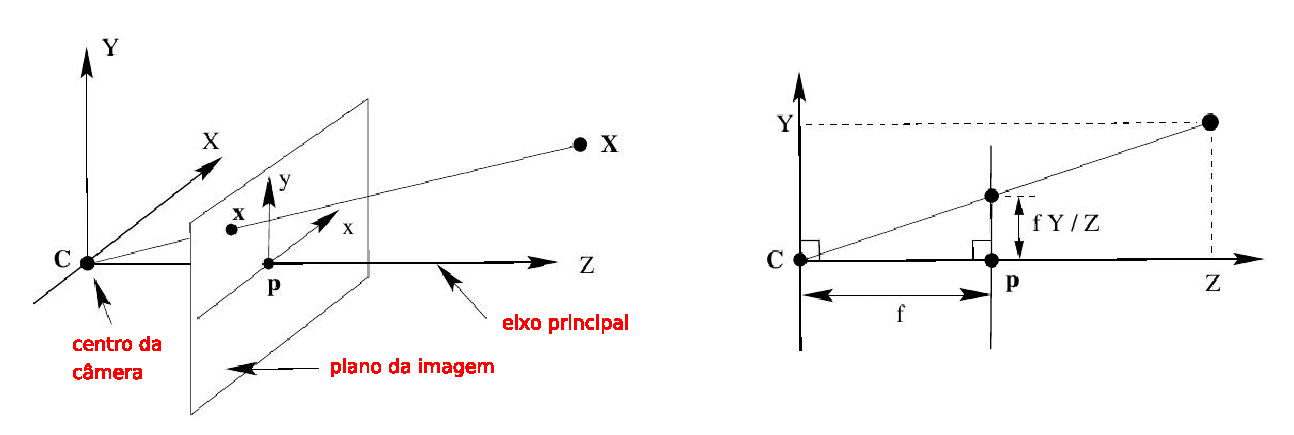
\includegraphics[width=\hsize]{modelo_camera}
\legend{Visualização das características básicas de uma câmera como distância focal, eixo principal, plano da imagem, centro de projeção e o ponto principal {\bf P}.}
\source{Adaptado, Hartley e Zisserman (2004).}
\label{camera}
\end{figure}
Com vetores representados em coordenadas homogêneas, podemos expressar o mapeamento através de um operador linear, onde realizamos a multiplicação da matriz $P$, que representa a câmera, por um ponto no espaço, resultando num ponto na imagem conforme o esquema abaixo:
\begin{center}
$
\begin{array}{ccc}
\begin{pmatrix}
fX\\
fY\\
Z
\end{pmatrix} = 
&
\begin{bmatrix}
f& & &0\\
 &f& &0\\
 & &1&0
\end{bmatrix}
&
\begin{pmatrix}
X\\
Y\\
Z\\
1
\end{pmatrix}.
\end{array}
$
\end{center}
Nessa matriz temos que $f$ é a distância focal (entre o centro da câmera e o plano da imagem), e o vetor de coluna de zeros à direita representa as coordenadas do centro da câmera, que nesse caso está na origem do sistema. Essa matriz pode ser desmembrada da seguinte maneria: uma matriz diagonal $diag(f,f,1)$ multiplicada pela matriz $[I|{\bf 0}]$, onde $I$ é uma matriz identidade $3\times3$ e ${\bf 0}$ é um vetor coluna de zeros. Compactamente, podemos escrever a última relaçao como:
\begin{center}
$\x = diag(f,f,1)\,[I|{\bf 0}]\,\X$,
\end{center}
onde $diag(f,f,1)\,[I|{\bf 0}]$ é a matriz da câmera para o modelo \textit{pinhole}.

Nessa dedução, consideramos que o ponto principal  coincide com a origem do plano da imagem, mas na prática isso pode não acontecer. Dessa forma, devemos acrescentar as coordenadas do ponto na construção da matriz da câmera. Sendo $(p_x,p_y)$ as coordenadas do ponto principal, desejamos o seguinte mapeamento (em coordenadas não homogêneas):
\begin{center}
$(X,Y,Z)^\top \rightarrow (\frac{f\,X}{Z}+p_x\,,\,\frac{f\,Y}{Z}+p_y)$,
\end{center}
o qual nos fornece a seguinte relação de projeção em coordenadas homogêneas:
\begin{center}
$
\begin{array}{ccc}
\begin{pmatrix}
f\,X + Z\,p_x\\
f\,Y + Z\,p_y\\
Z
\end{pmatrix}=
&
\begin{bmatrix}
f& &p_x&0\\
 &f&p_y&0\\
 & &1&0
\end{bmatrix}
\begin{pmatrix}
X\\
Y\\
Z\\
1
\end{pmatrix}
\end{array}
$
\end{center}
Definindo a notação
\begin{center}
$
\begin{array}{cc}
K = & \begin{bmatrix}
      f& &p_x\\
       &f&p_y\\
       & &1
      \end{bmatrix}, 
\end{array}
$
\end{center}
a relação de projeção assume a forma
\begin{equation}\label{eq.camera-incompleta}
\x=K\,[I|{\bf 0}]\,\X_{\textit{cam}},
\end{equation}
onde $K$ é denominada matriz de calibração da câmera, a qual resume os parâmetros internos da mesma, e $\X_{\textit{cam}}$ enfatiza que o ponto 3D está escrito no sistema de coordenadas da câmera.

A matriz de calibração $K$ ainda não está completa, pois o sistema de coordenadas do plano da imagem é medido em pixels, que podem ser não quadrados, e além disso os eixos cartesianos desse sistema podem ser não ortogonais. Assim, vamos inserir mais dois parâmetros para definir a medição em pixels e mais um parâmetro para definir o ângulo de inclinação entre os eixos cartesianos.

Sendo $m_x$ e $m_y$ a quantidade de pixels nas direções $x$ e $y$, respectivamente, a transformação para a coordenadas em pixels se dá pela multiplicação da matriz $diag(m_x,m_y,1)$ à esquerda da matriz $K$,
\begin{equation*}
\begin{bmatrix}
m_x&0&0\\
0&m_y&0\\
0&0&1
\end{bmatrix}      
\begin{bmatrix}
f& &p_x\\
&f&p_y\\
& &1
\end{bmatrix}
=
\begin{bmatrix}
\alpha_x&0&x_0\\
0&\alpha_y&y_0\\
0&0&1
\end{bmatrix}
\end{equation*}
onde $\alpha_x=m_x\,f$, $\alpha_y=m_y\,f$ representa a distância focal em termos das dimensões dos pixels. Similarmente, $x_0=m_x\,p_x$ e $y_0=m_y\,p_y$ são as coordenadas do ponto principal medidas em pixels. Para completar a generalidade, acrescentamos o parâmetro $s$, referente à inclinação entre os eixos, na matriz
\begin{equation*}
K=
\begin{bmatrix}
\alpha_x&s&x_0\\
0&\alpha_y&y_0\\
0&0&1
\end{bmatrix}.
\end{equation*}
Até aqui temos expressado o ponto $\X$ no espaço em relação às coordenadas da câmera, assumindo que o centro da câmera está situado na origem do sistema de eixos, o qual recebe o nome de sistema de coordenadas da câmera. Mas na maioria das vezes esse não é o caso, portanto desejamos fazer o mapeamento de um ponto 3D cujo as coordenadas estejam expressas com relação a um sistema de coordenadas qualquer, chamado sistema de coordenadas do mundo. Vamos continuar completando a matriz $P$ para mapear pontos no sistema de coordenadas do mundo.

Considerando o sistema de coordenadas do mundo, denotaremos um ponto nesse sistema, em coordenadas não homogêneas, por $\overline{\X}$, e o mesmo ponto no sistema de coordenadas da câmera será denotado por $\overline{\X}_{\textit{cam}}$. A transferência de sistemas de coordenadas é feita através da relação $\overline{\X}_{\textit{cam}}=R\,(\overline{\X}-\overline{\bf C})$, onde $\overline{\bf C}$ representa o centro da câmera no sistema de coordenadas do mundo e $R$ representa uma matriz de rotação $3\times3$. Passando os vetores para coordenadas homogêneas, podemos aplicar a rotação no vetor $\overline{\bf C}$, do centro da câmera, e inseri-lo na quarta coluna da matriz escrevendo a relação
\begin{center}
$
\begin{array}{ccc}
\X_{\textit{cam}}=
&
\begin{bmatrix}
R&-R\,\overline{\bf C}\\
\,\,{\bf 0}^\top&\,\,1
\end{bmatrix}
&
\begin{pmatrix}
X\\
Y\\
Z\\
1
\end{pmatrix},
\end{array}
$
\end{center} 
onde podemos escrever
\begin{center}
$
\begin{array}{cccc}
R=
&
\begin{bmatrix}
a&b&c\\
d&e&f\\
g&h&i
\end{bmatrix}
&
\qquad\text{e}\qquad
&
-R\,\overline{\bf C}=(t_1,t_2,t_3)^\top,
\end{array}
$
\end{center}
e a relação acima fica:
\begin{center}
$
\begin{array}{ccc}
\X_{\textit{cam}}=
&
\begin{bmatrix}
a&b&c&t_1\\
d&e&f&t_2\\
g&h&i&t_3\\
0&0&0&\,1
\end{bmatrix}
&
\begin{pmatrix}
X\\
Y\\
Z\\
1
\end{pmatrix}.
\end{array}
$
\end{center}
Substituindo $\X_{\textit{cam}}$ na Equação \ref{eq.camera-incompleta}, obtemos
\begin{center}
$
\begin{array}{ccccc}
\x=
&
\begin{bmatrix}
\alpha_x&s&x_0\\
0&\alpha_y&y_0\\
0&0&1
\end{bmatrix}&
\begin{bmatrix}
1&0&0&0\\
0&1&0&0\\
0&0&1&0
\end{bmatrix}
&
\begin{bmatrix}
a&b&c&t_1\\
d&e&f&t_2\\
g&h&i&t_3\\
0&0&0&\,1
\end{bmatrix}
&
\begin{pmatrix}
X\\
Y\\
Z\\
1
\end{pmatrix},
\end{array}
$
\end{center}
multiplicando a segunda e terceira matrizes,
\begin{center}
$
\begin{array}{cccc}
\x=
&
\begin{bmatrix}
\alpha_x&s&x_0\\
0&\alpha_y&y_0\\
0&0&1
\end{bmatrix}&
\begin{bmatrix}
a&b&c&t_1\\
d&e&f&t_2\\
g&h&i&t_3
\end{bmatrix}
&
\begin{pmatrix}
X\\
Y\\
Z\\
1
\end{pmatrix},
\end{array}
$
\end{center}
que pode ser escrita de forma resumida como
\begin{center}
$
\x=K\,[R|{\bf t}]\,\X,
$
\end{center}
com ${\bf t}=(t_1,t_2,t_3)^\top$ denominado vetor de translação.

Acabamos de incluir todos os parâmetros na matriz $P=K\,[R|{\bf t}]$, para o mapeamento de um ponto 3D homogêneo no sistema de coordenadas do mundo em seu respectivo ponto 2D no plano da imagem, no sistema de coordenadas da imagem. Temos cinco parâmetros internos na matriz de calibração $K$, $(\alpha_x,\alpha_y,s,p_x,p_y)$, três parâmetros externos na matriz de rotação $R$, apesar de suas nove entradas, e mais três parâmetros externos no vetor de translação totalizando 11 graus de liberdade. Repare que, tendo a matriz $P$ dimensão $3\times4$, ela possui 12 componentes e, usando uma para determinar a escala, sobram exatamente os 11 graus de liberdade, e a câmera $P$ é chamada câmera de \textit{projeção finita}.

\section*{A matriz de calibração K.}

A intenção nesta seção é mostrar qual é a natureza de cada um dos parâmetros internos da matriz de calibração. Para isso, vamos resolver o problema de transferir um ponto qualquer no espaço (em coordenadas não homogêneas) para o plano da imagem na câmera, conforme encontrado em \cite{tese-fabbri}.

\paragraph*{Problema:} Dado um ponto 3D $p^w = (x^w,y^w,z^w)^\top$ em coordenadas do mundo e sendo $(\uu,\vv)$ as coordenadas do ponto na imagem da câmera, quais os valores de $(\uu,\vv)$?\\

Primeiramente, vamos transformar o ponto em coordenadas do mundo para as coordenadas da câmera, $p = (x,y,z)^\top$ e
\begin{align*}
p = R p^w + T
\end{align*}
onde $R$ e $T$ são parâmetros extrínsecos. Agora, vamos projetar o ponto para o plano imagem normalizada usando similaridade de triângulos
\begin{empheq}[left=\empheqlbrace]{align*}\label{eq:normalized:coords}
\tilde x = \frac{x}{z}\\
\tilde y = \frac{y}{z}
\end{empheq}

Depois dessa projeção, vamos aplicar os parâmetros internos para obtermos as coordenadas finais da imagem. O primeiro passo é incluir a distância focal.
\begin{empheq}[left=\empheqlbrace]{align*}
\tilde x &= f\frac{x}{z}\\
\tilde y &= f\frac{y}{z}
\end{empheq}
Então converter para pixels:
\begin{empheq}[left=\empheqlbrace]{align*}
\tilde x_{pix} &= s_\uu f\frac{x}{z}\\
\tilde y_{pix} &= s_\vv f\frac{y}{z},
\end{empheq}
onde $s_\uu$ e $s_\vv$ é a quantidade de pixels por unidade de comprimento nas direções $\uu$ e $\vv$, respectivamente. Como podemos ver, $f$ tem efeito similar a $s_\uu$ e $s_\vv$. Seria suficiente mantermos apenas dois parâmetros, digamos $f$ e a razão de aspecto $\frac{s_\uu}{s_\vv}$, mas vamos manter os três parâmetros por enquanto.
%
%
Em seguida, fazemos a translação para o ponto inferior esquerdo da imagem usando $(t_{\tilde \uu},t_{\tilde \vv})$, que são as coordenadas do ponto principal em relação ao inferior esquerdo da imagem:
\begin{empheq}[left=\empheqlbrace]{align*}
\tilde \uu &= s_\uu f\frac{x}{z} + t_{\tilde \uu}\\
\tilde \vv &= s_\vv f\frac{y}{z} + t_{\tilde \vv},
\end{empheq}
e convertemos para o sistema de coordenadas em função de um ângulo $\theta$ entre os eixos, pois os eixos podem ser não ortogonais. Observe na Figura \ref{skew} a conversão das coordenadas de um ponto $Q$ qualquer:
\begin{figure}[!htb]{10cm}
\caption{Mudança de coordenadas.}
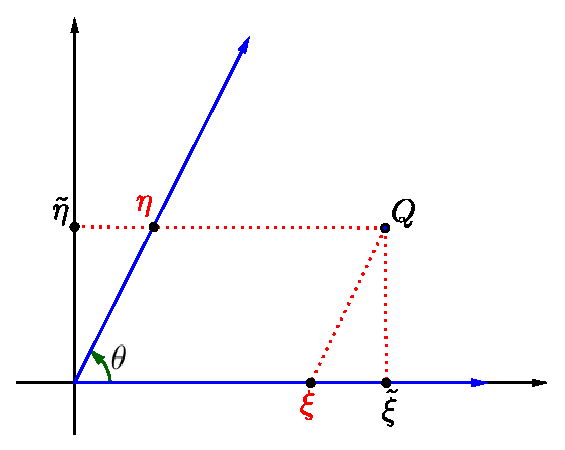
\includegraphics[width=\hsize]{skew}
\legend{Transformação das coordenadas de um ponto no plano com eixos perpendiculares para um plano com eixos relacionados por um ângulo $\theta$ qualquer.}
\source{O autor.}
\label{skew}
\end{figure}
\begin{empheq}[left=\empheqlbrace]{align*}
\tilde \uu &= \uu + \vv \, \cos\,\theta
\\
\tilde \vv &= \vv \, \sin\,\theta
\end{empheq}
Isolando as variáveis do sistema de coordenadas com ângulo genérico temos:
\begin{empheq}[left=\empheqlbrace]{align*}
\uu &= \tilde \uu - \tilde \vv \cot\theta \\
\vv &= \tilde \vv \,\csc\, \theta
\end{empheq}
os quais fornecem
\begin{empheq}[left=\empheqlbrace]{align*}\label{eq:projection:explicit}
\uu &= \overbrace{s_\uu f}^{\alpha_\uu}\frac{x}{z} + \overbrace{(-\cot\theta\, s_\vv
f)}^{\sigma_\theta} \frac{y}{z} + \overbrace{t_{\tilde \uu} - \cot\theta\, t_{\tilde \vv}}^{\uu_0}\\
%
\vv &= \underbrace{s_\vv f\,\csc\,\theta}_{\alpha_\vv} \frac{y}{z}+
\underbrace{\csc\,\theta\, t_{\tilde \vv}}_{\vv_0}
\end{empheq}
Assim, a transformação de um ponto expresso nas coordenadas da câmera para a imagem é feita usando cinco parâmetros da matriz de calibração
\begin{equation*}
K = \begin{bmatrix}
\alpha_\uu & \sigma & \uu_o\\
0 &\alpha_\vv &  \vv_o\\
0 & 0 &  1
\end{bmatrix}.
\end{equation*}
A fórmula acima explicita a interpretação de cada um desses parâmetros.
\begin{table}[!ht]{\textwidth}
  \caption{Resumo dos parâmetros da câmera.}\label{mais.rotulo}
  \hfill\begin{tabular}{c l}
      \textbf{Variáveis Livres} & \textbf{Descrição}\\
3	 & rotação \\
3	 & translação \\
2	 & mudança de escala em $x,y$\\
1	 & distância focal (pode ser incorporada como escala)\\
2	 & ponto principal\\
1	 & ângulo entre os eixos \\
6  & total extrinsecos\\
6  & total intrinsecos\\
12 & total\\
11 & total único (distância focal para fixar escala)
  \end{tabular}\hfill
  \source{O autor.}
\end{table}
\section{A ação projetiva de uma câmera $P$}
Nesta subseção iremos verificar como se dá a projeção aplicada por uma câmera $P$ em planos, retas, cônicas e quádricas.
\section*{Ação projetiva de $P$ em planos.}
A equação de projeção $\x=P\,\X$ é uma transformação de um ponto em coordenadas 3D no sistema de coordenadas do mundo para pontos 2D no sistema de coordenadas do plano da imagem na câmera e, por conta das características invariantes sob transformação projetiva, temos a liberdade para escolher o sistema de coordenadas do mundo. Assim, suponha que tal sistema de coordenadas seja posicionado de forma que o plano $xy$ corresponda ao plano $\bpi$, conforme ilustrado na Figura \ref{fig.projecao-planos-retas}. Desta forma, pontos no espaço que pertençam ao plano $\bpi$ terão a componente $X_3=0$, e a ação de uma câmera $P$ nesses pontos é dada por
\begin{equation*}
\begin{array}{rcl}
\x&=&P\,\X\\
&=&
\begin{pmatrix}
{\bf p_1}&{\bf p_2}&{\bf p_3}&{\bf p_4}
\end{pmatrix}
\begin{pmatrix}
X_1\\
X_2\\
0\\
1
\end{pmatrix}\\
&=&
\begin{pmatrix}
{\bf p_1}&{\bf p_2}&{\bf p_4}
\end{pmatrix}
\begin{pmatrix}
X_1\\
X_2\\
1
\end{pmatrix},
\end{array}
\end{equation*}
onde ${\bf p_i}$ são as colunas da matriz $P$. Assim, a transformação de um ponto $\X_\pi=(X_1,X_2,1)^\top\in\bpi$ para um ponto na imagem é, em geral, uma homografia planar, ou uma transformação projetiva de plano a plano $\x=H\,\X_\pi$.
\begin{figure}[htb!]{\textwidth}
\caption{Transformação plano a plano.}
\subfloat[]{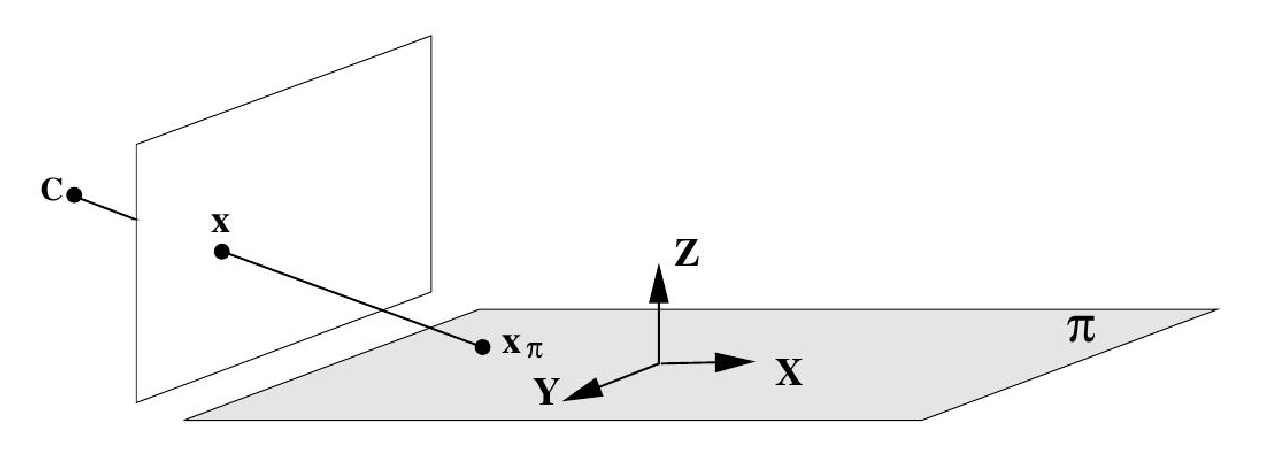
\includegraphics[scale=.5]{projecao-planos}}\hfill
\subfloat[]{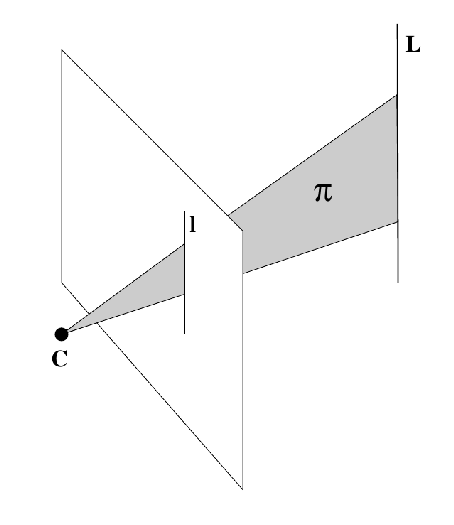
\includegraphics[scale=.5]{projecao-retas}}\hfill
\legend{({\tt a})Transformação projetiva de plano a plano induzida pela câmera $P$.\,\,({\tt b})Plano $\bpi$ retroprojetado por uma reta $\lightrgb$ no plano da imagem através da câmera $P$.}
\source{Hartley e Zisserman (2004).}
\label{fig.projecao-planos-retas}
\end{figure}
\subsection{A ação projetiva de $P$ em retas}\label{sec.proj.retas}
Geometricamente, como podemos ver na Figura \ref{fig.projecao-planos-retas}, uma reta ${\bf L}$ no espaço 3D junto com o centro $\C$ da câmera definem um plano. A interseção desse plano com o plano da imagem é uma reta $\lightrgb$, que é a imagem da reta ${\bf L}$ no espaço. Algebricamente, considere uma reta ${\bf L}$ parametrizada por $\lambda$ passando pelos pontos ${\bf A}$ e ${\bf B}$, onde cada ponto nessa reta é dado por $\X(\lambda)={\bf A}+(\lambda)\,{\bf B}$. Considere ainda, ${\bf a}$ e ${\bf b}$ sendo as imagens dos pontos ${\bf A}$ e ${\bf B}$ sob a ação da câmera $P$. Aplicando a projeção da câmera $P$ aos pontos da reta ${\bf L}$ temos
\begin{equation*}
\begin{array}{rcl}
\x(\lambda)&=&P\,\X(\lambda)\\
&=&P({\bf A}+(\lambda)\,{\bf B})\\
&=&P\,{\bf A}+(\lambda)\,P\,{\bf B}\\
&=&{\bf a}+(\lambda)\,{\bf b},
\end{array}
\end{equation*}
onde cada $\x$ em função de $\lambda$ pertence à reta passando por ${\bf a}$ e ${\bf b}$ no plano da imagem.  
\section*{Retroprojeção de retas.}
Geometricamente, a retroprojeção de retas é o conjunto de pontos no espaço pertencentes a um plano, o qual é definido pelo centro da câmera e uma reta na imagem, como na Figura \ref{fig.projecao-planos-retas}. Algebricamente, sendo a reta na imagem denotada por $\lightrgb$ e a câmera por $P$, o plano retroprojetado é $P^\top\lightrgb$. De fato, um ponto $\X$ no espaço é projetado na imagem como $\x=P\,\X$, e esse ponto pertence a reta $\lightrgb$ na imagem se $\x^\top\lightrgb=0$ ou, substituindo, $(P\,\X)^\top\lightrgb=0$. Então, aplicando a transposta, $\X^\top P^\top\lightrgb=0$ e $P^\top\lightrgb$ é tomado como o plano que contém o ponto $\X$ no espaço. Assim, tal plano é a retroprojeção da reta $\lightrgb$.  
\section*{A ação projetiva de $P$ em cônicas.}
Um cone é uma quádrica degenerada, representada por uma matriz $4\times4$ que não tem posto completo, e é denotada por ${\tt Q}_{co}$.
\section*{Retroprojeção de cônicas.}
Uma cônica retroprojeta um cone ${\tt Q}_{co}$ que, neste caso, tem o vértice coincidindo com o centro da câmera, onde esse vértice é o vetor nulo da matriz $4\times4$ que representa o cone. Uma cônica retroprojeta um cone de acordo com 
\begin{equation*}
{\tt Q}_{co}=P^\top C\,P
\end{equation*}
pois, um ponto $\X$ no espaço é projetado na imagem na forma $\x=P\,\X$, e $\x\in C$ se satisfaz a equação $\x^\top C\,\x=0$. Substituindo $\x$ na equação da cônica temos $(P\,\X)^\top C\,P\,\X=0$, e aplicando a transposição, $\X^\top P^\top C\,P\,\X=0$. O ponto $\X$ é projetado na cônica $C$ se , se e somente se, $\X\in {\tt Q}_{co}$, que deve ser definida como ${\tt Q}_{co}=P^\top C\,P$. Assim, um cone é a retroprojeção de uma cônica, e repare que não há a projeção direta de uma cônica, já que uma cônica é definida por uma matriz $3\times3$ e a matriz da câmera é $3\times4$.
\subsection{A ação projetiva de $P$ em quádricas}\label{sec.proj-quadricas}
Para tratarmos desse assunto, primeiramente precisamos definir alguns conceitos.
\section*{Contorno gerador e contorno aparente.}
Na formação da imagem de uma superfície, os raios de luz passando pelo centro da câmera são tangentes à essa superfície em 3D. O contorno dessa superfície nesses pontos de tangência é transformado num contorno no plano da imagem conforme a Figura \ref{fig.cont-gerador-aparente}. O contorno da superfície é denominado \textit{contorno gerador} e denotado por ${\bf \Gamma}$, o contorno formado na imagem é chamado \textit{contorno aparente} e denotado por ${\bf \gamma}$. Vale ressaltar que o contorno gerador depende das posições do centro da câmera e da própria superfície, e não depende do plano da imagem.
\begin{figure}[htb!]{\textwidth}
\caption{Contornos de qu\'adricas.}
\subfloat[]{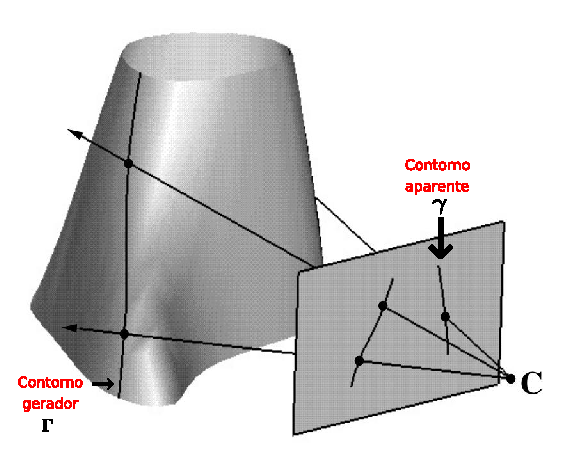
\includegraphics[scale=.91]{contorno-gerador-aparente}}\hfill
\subfloat[]{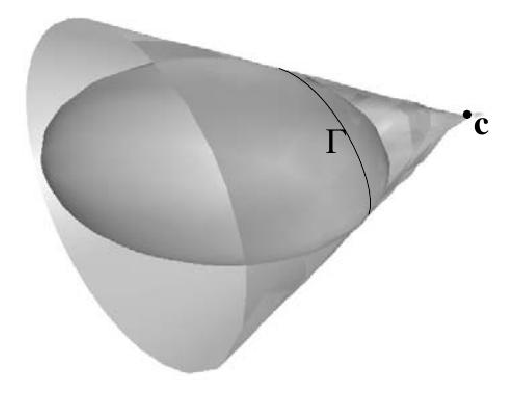
\includegraphics[scale=.91]{superficie-lisa}}\hfill
\legend{$({\tt a})\,$ O contorno aparente é a imagem do contorno gerador.$\,\,({\tt b})\,$ Uma quádrica tangenciada por um cone que é o formado pelo conjunto de retas passando pelo centro da câmera, onde tais retas são tangentes ao contorno gerador ${\bf \Gamma}$. }
\source{Hartley e Zisserman (2004).}
\label{fig.cont-gerador-aparente}
\end{figure}
\section*{Projeção de quádricas.}
A quádrica é uma superfície lisa  e o seu contorno gerador produz um contorno aparente no plano da imagem, através dos raios retroprojetados pelos pontos do contorno aparente e passando pelo centro da câmera, conforme um exemplo na Figura \ref{fig.cont-gerador-aparente}. Assim, o contorno gerador é uma cônica e sob uma transformação projetiva o contorno aparente também é uma cônica na imagem. Como estamos usando relações de tangência aos contornos gerador e aparente, será necessária a utilização da quádrica dual	${\tt Q}^*$, já que por definição a equação que representa a quádrica dual fica definida pelos planos $\bpi$ que são tangentes ao contorno gerador na quádrica ${\tt Q}$. Portanto, a equação da quádrica dual é dada por
\begin{equation*}
\bpi^\top {\tt Q}^*\bpi=0.
\end{equation*}
Sejam $\lightrgb$ as retas tangentes à conica $C$ na imagem (contorno aparente), onde a cônica dual define a relação $\lightrgb^\top C^*\lightrgb=0$. Essas retas $\lightrgb$ retroprojetam planos definidos por $\bpi=P^\top\lightrgb$ (Subseção \ref{sec.proj.retas}), que são tangentes à quádrica ${\tt Q}$ e satisfazem a relação $\bpi^\top {\tt Q}^*\bpi=0$. Substituindo o plano nessa última relação temos

\begin{equation*}
\begin{array}{rcl}
\bpi^\top {\tt Q}^*\bpi&=&(P^\top\lightrgb)^\top {\tt Q}^*P^\top\lightrgb\\
&=&\lightrgb^\top P\,{\tt Q}^*P^\top\lightrgb\\
&=&\lightrgb^\top C^*\lightrgb\\
&=&0,
\end{array}
\end{equation*}
onde tomamos $C^*=P\,{\tt Q}^*P^\top$, a imagem da quádrica sob a projeção $P$.

\subsection{A geometria bifocal}

\section*{A geometria epipolar.}

Considere um cenário com um ponto $\X$ no espaço 3D e dois planos que contêm as imagens $\x$ e $\x'$ desse ponto $\X$. Considere ainda um plano $\bpi$ que contém esse ponto $\X$ e os dois centros de projeção (ou centro da câmera) das duas câmeras, denotados por $\C$ e $\C'$. A geometria epipolar se constitui nas relações existentes entre as interseções desse plano $\bpi$ com os dois planos das imagens observado na Figura \ref{fig.geo-epipolar}. Sendo $\x$ a imagem 2D de $\X$ no primeiro plano de imagem, a construção desse cenário é motivada pela busca de $\x'$, também 2D, que seja correspondente a $\x$, onde $\x'$ é a imagem de $\X$ no segundo plano de imagem. Ou seja, existem as matrizes que promovem a ação de cada câmera onde $\x=P\,\X$ e $\x'=P'\,\X$, e quando isso acontece dizemos que os pontos são {\it pontos correspondentes}, e denotamos por $\x\leftrightarrow\x'$ (já definidos anteriormente). Podemos observar que $\x$ e $\x'$ retroprojetam duas retas definidas por $\C$ e $\C'$, onde esses retas pertencem a $\bpi$ e se interceptam em $\X$. Essa propriedade é essencial para nos auxiliar a definir as correspondências entre os pontos nas duas imagens. 

A \textit{reta base} é a reta que passa pelo centro de cada câmera $\C$ e $\C'$. O plano $\bpi$ fica determinado pela reta base e pela reta definida por $\x$ e $\C$. A interseção de $\bpi$ com o segundo plano de imagem define uma reta chamada \textit{reta epipolar}, que é a imagem na segunda visão da reta retroprojetada por $\x$. Ou seja, dadas duas imagens de uma cena, para cada ponto numa imagem vai existir uma reta epipolar correspondente na outra imagem. Pela construção, sabemos que $\x'\in\bpi$ e pertence ao plano da segunda imagem, portanto $\x'$ pertence à reta epipolar que será denotada por $\lightrgb'$. Assim, nossa busca pela correspondência de $\x$ se restringirá a uma busca numa reta e não a uma busca em todo o plano de imagem da segunda câmera. 
\begin{equation*}
\x\rightarrow\lightrgb'
\end{equation*}
A imagem do centro de projeção da primeira câmera na segunda fotografia é denominada \textit{epipolo} e denotada por $\e'$. Analogamente, a imagem de $\C'$ na primeira fotografia também é chamada epipolo e é denotada por $\e$.
O plano $\bpi$ é denominado \textit{plano epipolar} e num sistema com duas vistas temos vários planos epipolares definidos por um único parâmetro, e que formam o feixe de planos girando em torno da reta base.
\begin{figure}[!htb]{.75\textwidth}
\caption{O plano epipolar.}
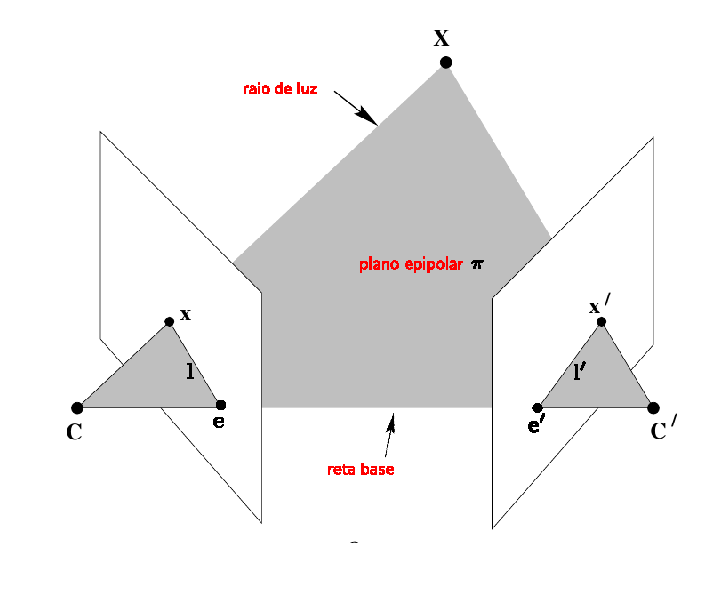
\includegraphics[width=\hsize]{geometria-epipolar}
\source{Adaptado, Hartley e Zisserman (2004).}
\label{fig.geo-epipolar}
\end{figure}
\subsection{A homografia induzida por um plano}\label{sec.homografia}

Considere um plano $\bpi$ no espaço 3D com coordenadas expressas em um referencial no mundo, com duas câmeras, mas que não passa pelo centro de nenhuma das duas câmeras. Portanto esse plano não é um plano epipolar e é dito estar em posição geral. Assim, vamos determinar uma homografia definida em função desse plano $\bpi$.\\

Dadas as duas matrizes de projeção canônicas
\begin{equation*}
P=[I|{\bf 0}]\qquad\text{e}\qquad P'=[R|{\bf t}],
\end{equation*}
(as câmeras não são calibradas pois não possuem a matriz $K$ e a origem do sistema cartesiano do mundo coincide com o centro da primeira câmera) um plano $\bpi=({\bf v},1)^\top$, e um ponto $\X\in\bpi$, então a homografia induzida por $\bpi$ é
\begin{equation*}
\x'=H\,\x,\qquad\text{onde}\qquad H=R-{\bf t}\,{\bf v}^\top.
\end{equation*}
Podemos tomar a última coordenada de $\bpi$ igual a $1$, pois nos interessa apenas que o plano não passe pelo centro da primeira câmera $\C=(0,0,0,1)^\top$. Observe o esquema na Figura \ref{fig.homografia}.

Na primeira câmera temos a projeção
\begin{equation*}
\x=P\,\X=[I|{\bf 0}]\,\X,
\end{equation*}
e qualquer ponto 3D do tipo $\X=(\x^\top,\rho)^\top$ vai satisfazer a projeção acima. De fato
\begin{equation*}
P\,\X=
[I|{\bf 0}]\,(\x^\top,\rho)^\top=
\begin{bmatrix}
1&0&0&0\\
0&1&0&0\\
0&0&1&0
\end{bmatrix}
\begin{pmatrix}
x_1\\
x_2\\
x_3\\
\rho
\end{pmatrix}
=\x,
\end{equation*}
e assim qualquer ponto na reta retroprojetada por $\x$ pode ser parametrizado por $\rho$. Como $\X\in\bpi$, $\bpi^\top\X=0$ e  
$\rho$ fica determinado
\begin{equation*}
\begin{array}{rcl}
\bpi^\top\,\X&=&0\\
({\bf v}^\top,1)\,(\x^\top,\rho)^\top&=&0\\
{\bf v}^\top\x+\rho&=&0\\
\rho&=&-{\bf v}^\top\,\x,
\end{array}
\end{equation*}
e dessa forma o ponto $\X=(\x^\top,-{\bf v}^\top\x)^\top$.
Projetando o ponto 3D na segunda imagem temos
\begin{equation*}
\begin{array}{rcl}
\x'&=&P'\X\\
&=&[R|{\bf t}]\,(\x^\top,-{\bf v}^\top\x)^\top\\
&=&R\,\x-{\bf t}\,{\bf v}^\top\x\\
&=&(R-{\bf t}\,{\bf v}^\top)\,\x.
\end{array}
\end{equation*}
Portanto
\begin{equation*}
\x'=H\,\x,\qquad\text{onde}\qquad H=R-{\bf t}\,{\bf v}^\top.
\end{equation*}
\begin{figure}[!htb]{.8\textwidth}
\caption{Homografia planar.}
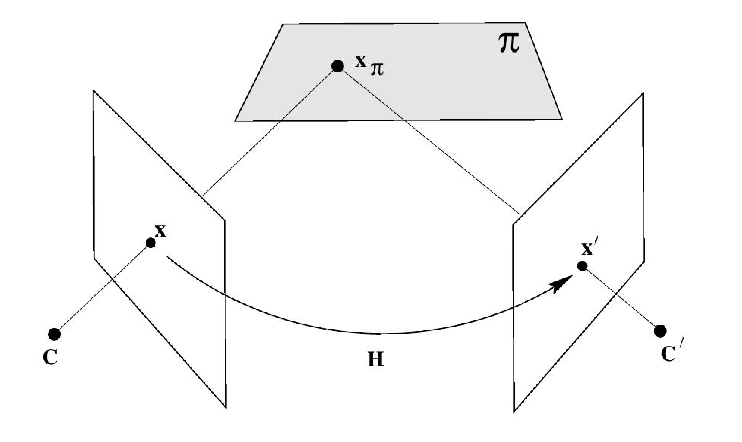
\includegraphics[width=\hsize]{homografia}
\source{Hartley e Zisserman (2004).}
\label{fig.homografia}
\end{figure}
\subsection{A matriz fundamental $F$}\label{sec.matriz-F}

A \textit{matriz fundamental} reúne todas as informações da geometria epipolar, é a representação algébrica dessa geometria espacial com duas câmeras e, por isso, também é conhecida como \textit{tensor bifocal}. 

Geometricamente, a matriz fundamental pode ser obtida através do mapeamento de $\x$ na primeira imagem a um ponto $\x'$ na segunda imagem utilizando um plano $\bpi$ qualquer no espaço. Após esse mapeamento, identificamos a reta epipolar definida pelos pontos $\x'$ e $\e'$. Assim, considere um plano $\bpi$ que não passe pelos centros das câmeras, pois desse jeito uma reta retroprojetada por $\x$ deve interceptar o plano $\bpi$ em algum ponto $\X$. Usando a transferência através do plano $\bpi$, o ponto $\X$ deve ser projetado a um ponto $\x'$ na segunda imagem e, como $\X$ pertence à reta retroprojetada por $\x$, o ponto $\x'$ deverá pertencer à reta epipolar $\lightrgb'$, já que $\lightrgb'$ é a imagem na segunda câmera da reta retroprojetada por $\x$ conforme a Figura \ref{fig.geo-epipolar}. Assim, pela Subseção \ref{sec.homografia} existe uma homografia 2D $H$ em função de $\bpi$ onde cada ponto $\x_i$ é mapeado a um ponto $\x_i'$, 
\begin{equation}\label{eq.homo-plano}
\x'_i= H_{\bpi} \,\x_i.
\end{equation}
Tais pontos são ditos projetivamente equivalentes, já que são projetivamente equivalentes a um mesmo ponto $\X_i$ no plano $\bpi$. Obtido o ponto $\x'$, a reta epipolar passando por $\x'$ e $\e'$ pode ser calculada fazendo 
\begin{equation}\label{eq.reta-epi-pro-vet}
\begin{array}{rcl}
\lightrgb'&=&\e'\times\x'\\
&=&[\e']_\times\x'.
\end{array}
\end{equation}
Substituindo \ref{eq.homo-plano} em \ref{eq.reta-epi-pro-vet} temos
\begin{equation*}
\begin{array}{rcl}
\lightrgb'&=&[\e']_\times\x'\\
&=&[\e']_\times H_{\bpi} \,\x\\
&=&F\,\x,
\end{array}
\end{equation*} 
onde definimos $F=[\e']_\times H_{\bpi}$ é a matriz fundamental. Como $[\e']_\times$ é uma matriz anti-simétrica $3\times3$ obtida de um vetor, então  $[\e']_\times$ tem posto $2$ e como $H_{\bpi}$ obtida de um plano tem posto $3$, temos que a matriz fundamental tem posto $2$. $F$ é o mapeamento de um plano projetivo a um feixe de retas epipolares.


Algebricamente, a matriz fundamental pode ser determinada a partir das matrizes das duas câmeras $P$ e $P'$. Vamos primeiramente definir a equação que representa a reta retroprojetada por $\x$. Dado um ponto $\x$ na imagem, precisamos determinar o conjunto de pontos no espaço 3D que são mapeados nesse ponto $\x$, e este raio de luz (modelado por uma reta) será definido pela junção de dois de seus pontos. E conhecemos dois pontos pertencentes a esta reta, $\C$ é o centro da câmera tal que $P\,\C={\bf 0}$, e o ponto $P^+\x$ onde $P^+$ é a pseudo-inversa de $P$ definida na Subseção \ref{sec.Apen-A}. O ponto $P^+\x$ pertence à reta retroprojetada por $\x$ pois aplicando-lhe a projeção efetuada pela câmera temos o próprio ponto $\x$ como retorno:
\begin{equation*}
P^+\x \rightarrow P\,P^+\x=I\,\x=\x.
\end{equation*}
Portanto, podemos formar a reta pela junção dos pontos $\C$ e $P^+\x$, parametrizada por $\lambda$
\begin{equation*}
\X(\lambda)=P^+\x+\lambda\,\C.
\end{equation*}
Computando a imagem desses dois pontos na segunda câmera temos
\begin{equation*}
\begin{array}{c}
P^+\x \rightarrow P'P^+\x\\
\C \rightarrow P'\C,
\end{array}
\end{equation*}
onde $P'\,\C$ é o epipolo na segunda imagem, e por isso, a reta epipolar pode ser definida em termos do produto vetorial desses dois pontos
\begin{equation}\label{eq.reta-epipolar-funcao-cameras}
\lightrgb'=P'\C \times P'P^+\x.
\end{equation}
Mas como $P'\C=\e'$, podemos substitui-lo na equação anterior
\begin{equation*}
\begin{array}{rcl}
\lightrgb'&=&P'\C \times P'P^+\x\\
&=&[\e']_\times P'P^+\x\\
&=&F\,\x,
\end{array}
\end{equation*}
definindo $F=[\e']_\times P'P^+$. Essa relação para $F$ é a mesma fórmula derivada anteriormente, com a homografia planar calculada em termos das duas câmeras, $H_{\bpi}=P'P^+$.

Em problemas de reconstrução 3D podemos considerar a posição da primeira câmera como a origem do sistema de coordenadas do mundo, assim a matriz $P$, sua pseudo-inversa e a matriz da segunda câmera são, respectivamente 
\begin{equation*}
P=K\,[I|{\bf 0}],\qquad
P^+=
\begin{bmatrix}
K^{-1}\\
{\bf 0}^\top
\end{bmatrix}\qquad\text{e}\qquad
P'=K'[R|{\bf t}].
\end{equation*}
Substituindo na Equação \ref{eq.reta-epipolar-funcao-cameras} temos
\begin{equation*}
\begin{array}{rcl}
\lightrgb'&=&P'\C \times P'P^+\x\\
&=&K'[R|{\bf t}]
\begin{pmatrix}
0\\
0\\
0\\
1
\end{pmatrix}
\times K'[R|{\bf t}]
\begin{bmatrix}
K^{-1}\\
{\bf 0}^\top
\end{bmatrix}\x\\
&=&
[K'{\bf t}]_\times K'\,R\,K^{-1}\x,
\end{array}
\end{equation*}
onde teremos uma nova definição para a matriz fundamental 
\begin{equation}\label{eq.definicao-F}
F=[K'{\bf t}]_\times K'\,R\,K^{-1}.
\end{equation}
Essa definição para $F$ é importante para falarmos sobre a matriz {\it essencial}.
\subsection{Propriedades da matriz fundamental}\label{sec.propriedades-F}
A partir da função $\x\rightarrow\lightrgb'$ dada pela relação $\lightrgb'=F\,\x$, podemos derivar a propriedade mais básica da matriz fundamental.
Observe que se $\x'\in\lightrgb'\Rightarrow\x'^\top\lightrgb'=0$, e temos
\begin{equation*}
\begin{array}{rcl}
\lightrgb'&=&F\,\x\\
\x'^\top\lightrgb'&=&\x'^\top F\,\x\\
0&=&\x'^\top F\,\x.
\end{array}
\end{equation*}
A relação acima é denominda {\it condição de correspondência}, pois pontos que a satisfazem devem ser  coplanares e tal relação se mostra uma ferramenta para a determinação da matriz fundamental a partir dos pontos correspondentes $\x\leftrightarrow\x'$. Observe que essa forma de determinar $F$ não requer o conhecimento das câmeras $P$ e $P'$. 

Se $F$ é a matriz para as câmeras $(P,P')$ então $F^\top$ é a matriz para $(P',P)$, pois basta aplicar a transposição em 
\begin{equation*}
\begin{array}{rcl}
\x'^\top F\,\x&=&0\\
\x^\top F^\top\x'&=&0,\quad\text{onde}\quad F^\top\x'=\lightrgb.
\end{array}
\end{equation*}
Os epipolos $\e$ e $\e'$ são os espaços nulos à direita e à esquerda de $F$, respectivamente. Vimos que $\e'\in\lightrgb'\Rightarrow\e'^\top\lightrgb'=0$, e $\lightrgb'=F\,\x$ para todo ponto $\x\in\lightrgb$ (exceto $\e$), daí
\begin{equation*}
\begin{array}{rcl}
\lightrgb'&=&F\,\x\\
\e'^\top\lightrgb'&=&\e'^\top F\,\x\\
0&=&\e'^\top F\,\x,\quad\text{para todo}\,\,\x\\
{\bf 0}^\top&=&\e'^\top F.
\end{array}
\end{equation*} 
A dedução é análoga para $F\,\e={\bf 0}$.
\subsection{Configuração canônica das câmeras}\label{sec.cameras-canonicas}
A relação $\lightrgb'=F\,\x$ é uma relação projetiva, já que envolve apenas relacionamentos projetivos entre os objetos geométricos, como interseção de retas e planos, e no desenvolvimento algébrico envolve apenas a projeção realizada pela câmera entre pontos no mundo e pontos na imagem. Com isso, a relação depende apenas das coordenadas projetivas da imagem, ou seja, é projetivamente invariante. Assim, dadas transformações projetivas das imagens $\hat{\x}=H\,\x$ e $\hat{\x}'=H'\x'$ podemos deduzir a correspondente relação $\hat{\lightrgb}'=\hat{F}\hat{\x}$ com $\hat{F}=H'^{-\top}F\,H^{-1}$. Analogamente, $F$ depende somente das propriedades projetivas das câmeras $P$ e $P'$, já que as imagens são geradas pela ação dessas duas câmeras. As câmeras dependem tanto do sistema de coordenadas das imagens como do sistema de coordenadas do mundo, mas a matriz fundamental é inalterável por uma transformação projetiva do espaço 3D. 

Observe que se $H_{4\times4}$ é uma transformação projetiva do espaço 3D, então as relações de projeção podem ser escritas como
\begin{equation*}
\begin{array}{rcl}
\x&=&P\,\X\\
\x&=&P\,H\,H^{-1}\X
\end{array}\qquad\text{e}\qquad
\begin{array}{rcl}
\x'&=&P'\X\\
\x'&=&P'H\,H^{-1}\X
\end{array}.
\end{equation*} 
Se $\x\leftrightarrow\x'$ é uma correspondência para o par de câmeras $(P,P')$ em relação ao ponto $\X$, então essas imagens também são correspondentes para o par de câmeras $(P\,H,P'H)$ em relação ao ponto $H^{-1}\X$. Como a matriz fundamental depende apenas das coordenadas das imagens (Subseção \ref{sec.propriedades-F}), temos que a matriz fundamental para $(P,P')$ será a mesma para $(P\,H,P'H)$. Ou seja, um par de câmeras unicamente define uma matriz fundamental, mas uma matriz fundamental é consistente com vários pares de câmeras.

Já que temos vários pares de câmeras consistentes com a mesma matriz fundamental, podemos escolher um par de câmeras, através de uma transformação projetiva, de forma que algumas futuras abordagens e deduções sejam facilitadas sem prejuízo das características projetivas. Dadas câmeras calibradas $\hat{P}$ e $\hat{P'}$ podemos acrescentar uma linha em $\hat{P}$ de forma que se torne uma matriz $4\times4$ invertível denotada por $\hat{P}^*$. Aplicando a inversa de $\hat{P}^*$ em $\hat{P}$ e $\hat{P}'$ temos que
\begin{equation*}
\begin{array}{rcl}
P&=&\hat{P}\,\hat{P}^{*-1}\\
P&=&[I|{\bf 0}]
\end{array}\qquad\text{e}\qquad
\begin{array}{rcl}
P'&=&\hat{P}'\,\hat{P}^{*-1}\\
P'&=&[M|{\bf m}].
\end{array}
\end{equation*}
As câmeras $P$ e $P'$ definidas acima estão em sua forma {\it canônica}. Observe, pela dedução da Equação \ref{eq.definicao-F}, que a matriz fundamental para câmeras canônicas é simplesmente 
\begin{equation*}
F=[{\bf m}]_\times M.
\end{equation*}
\section*{Extraindo as câmeras canônicas a partir de $F$.}
Nesta seção será apresentada uma das formas de se obter as matrizes das câmeras para um sistema com duas visões. Como vimos na Subseção \ref{sec.cameras-canonicas}, é possível aplicar uma transformação projetiva de forma a se obter o par de câmeras canônicas para um sistema bifocal, e assim facilitar o algebrismo e a computação sem prejuízo das características projetivas do sistema. Desta forma, dada a matriz $F$ computada através da codição de correspondência, vamos mostrar como extrair o par de câmeras em sua forma canônica.

Primeiramente, observe pelo Apêndice \ref{sec.Apen-A} o caso $3\times3$ em que uma matriz $M$ é anti-simétrica se satisfaz a condição ${\bf v}^\top M\,{\bf v}=0$. Considerando a matriz $P'^\top F\,P$, a mesma será anti-simétrica se $\X^\top P'^\top F\,P\,\X=0$. Mas $\x=P\,\X$ e $\x'^\top=\X^\top P'^\top$, e substituindo temos que $\x'^\top F\,\x=0$. Pela Subseção \ref{sec.propriedades-F}, essa condição de correspondência mostra que $F$ é a matriz fundamental consistente com o par de câmeras $(P,P')$ já que $P'^\top F\,P$ seja anti-simétrica.

Agora, tomando a configuração canônica $P=[I|{\bf 0}]$ e $P'=[SF\,|\e']$, onde $S$ é uma matriz anti-simétrica e $\e'$ é o epipolo que satisfaz $\e'^\top F={\bf 0}^\top$ (Subseção \ref{sec.propriedades-F}), temos que $P'^\top F\,P$ é anti-simétrica, pois
\begin{equation*}
P'^\top F\,P=[SF\,|\e']^\top F\,[I|{\bf 0}]=
\begin{bmatrix}
F^\top S^\top F&{\bf 0}\\
\e'^\top F&0
\end{bmatrix}=
\begin{bmatrix}
F^\top S^\top F&{\bf 0}\\
{\bf 0}^\top&0
\end{bmatrix}.
\end{equation*}
Assim, dada $F$ temos que um par de câmeras consistente é simplesmente $P=[I|{\bf 0}]$ e $P'=[SF\,|\e']$. Repare que a escolha da matriz $S$ é arbitrária mas com a exigência de que a matriz $P'$ deve ter posto 3 para ser uma câmera válida. Isso não é problema pois segundo \cite{luong} uma boa escolha é $S=[\e']_\times$ pois $\e'$ não pertence ao espaço gerado pelas colunas de $[\e']_\times F$. Finalmente, o par de câmeras canônicas pode ser obtido tomando 
\begin{equation}\label{eq.cameras-dada-F}
P=[I|{\bf 0}]\qquad\text{e}\qquad P'=[[\e']_\times F\,|\e'].
\end{equation}
\subsection{Ambiguidade projetiva das câmeras, dada $F$}\label{sec.ambi-cameras-dada-F}

De uma matriz fundamental podemos extrair diferentes pares de câmeras consistentes com a mesma geometria epipolar, em contraste com o fato de, dado um par de câmeras, a matriz fundamental ser única. Esses pares de câmeras extraídas de $F$ diferem apenas por uma transformação projetiva.

Inicialmente, podemos aplicar uma transformação projetiva e trabalhar com a forma canônica das câmeras $P=\tilde{P}=[I|{\bf 0}]$, $P'=[A|{\bf a}]$ e $\tilde{P}'=[\tilde{A}|\tilde{{\bf a}}]$. Evocando o resultado em \ref{sec.cameras-canonicas} sabemos que a matriz fundamental pode ser obtida fazendo 
$F=[{\bf a}]_{\times} A=[\tilde{{\bf a}}]_{\times} \tilde{A}$. Como $[{\bf a}]_{\times}$ e $[\tilde{{\bf a}}]_{\times}$ são anti-simétricas temos que
\begin{equation*}
{\bf a}^\top F={\bf a}^\top [{\bf a}]_{\times} A={\bf 0}^\top\quad\text{e}\quad\tilde{{\bf a}}^\top F=\tilde{{\bf a}}^\top [\tilde{{\bf a}}]_{\times} \tilde{A}={\bf 0}^\top,
\end{equation*}
e como $F$ tem posto 2 e não pode ser invertida, temos que ${\bf a}^\top$ e ${\tilde{{\bf a}}^\top}$ são iguais a menos de escala, portanto
\begin{equation}\label{eq.dedu-ambiguidade-P-1}
{\tilde{{\bf a}}^\top}=k\,{\bf a}^\top.
\end{equation}
Considerando $[{\bf a}]_{\times} A=[\tilde{{\bf a}}]_{\times} \tilde{A}$ e substituindo a Equaç\~ao \ref{eq.dedu-ambiguidade-P-1} temos
\begin{equation*}
\begin{array}{rcl}
[{\bf a}]_{\times} A&=&k\,[{\bf a}]_{\times} \tilde{A}\\
0_{3\times3}&=&k\,[{\bf a}]_{\times} \tilde{A}-[{\bf a}]_{\times} A\\
0_{3\times3}&=&[{\bf a}]_{\times}(k\,\tilde{A}-A).
\end{array}
\end{equation*}
Já que ${\bf a}$ é um vetor nulo à direita de $[{\bf a}]_{\times}$ podemos tomar, para um vetor ${\bf v}$ qualquer,
\begin{equation}\label{eq.dedu-ambiguidade-P-2}
k\,\tilde{A}-A={\bf a}{\bf v}^\top\quad\text{e daí}\quad \tilde{A}=\frac{A+{\bf a}{\bf v}^\top}{k}. 
\end{equation}
Substituindo as Equações \ref{eq.dedu-ambiguidade-P-1} e \ref{eq.dedu-ambiguidade-P-2} na câmera $\tilde{P}'$ temos que 
\begin{equation}\label{eq.camera-geral}
P'=[A|{\bf a}]\quad\text{e}\quad \tilde{P}'=[k^{-1}(A+{\bf a}{\bf v}^\top)|k\,{\bf a}],
\end{equation}
e vamos usar a homografia
\begin{equation*}
H=
\begin{bmatrix}
k^{-1}I&{\bf 0}\\
k^{-1}{\bf v}^\top&k
\end{bmatrix}
\end{equation*}
para mostrar que as câmeras estão projetivamente relacionadas.
\begin{equation*}
PH=[I|{\bf 0}]
\begin{bmatrix}
k^{-1}I&{\bf 0}\\
k^{-1}{\bf v}^\top&k
\end{bmatrix}
=
k^{-1}[I|{\bf 0}]=k^{-1}\tilde{P},\quad\text{e}
\end{equation*}
\begin{equation*}
P'H=[A|{\bf a}]
\begin{bmatrix}
k^{-1}I&{\bf 0}\\
k^{-1}{\bf v}^\top&k
\end{bmatrix}
=
[k^{-1}(A+{\bf a}{\bf v}^\top)|k\,{\bf a}]
=[\tilde{A}|\tilde{{\bf a}}]=\tilde{P}'.
\end{equation*}
Juntando a extração das câmeras dada em \ref{eq.cameras-dada-F} com a equação geral para câmeras dada em \ref{eq.camera-geral} temos a fórmula geral para câmeras canônicas dada a matriz fundamental
\begin{equation*}
P=[I|{\bf 0}]\quad\text{e}\quad P'=[[\e']_\times F+\e'{\bf v}^\top |\lambda\,\e'],
\end{equation*} 
para um vetor ${\bf v}$ qualquer  e um escalar $\lambda\neq0$.
\section*{A matriz essencial $E$.}
Historicamente, a matriz essencial foi introduzida antes da matriz fundamental e pode ser pensada como um caso particular da matriz fundamental \cite{Longuet}, onde os efeitos da matriz de calibração $K$ foram removidos da câmera $P$. Considere uma câmera $P=K\,[R|{\bf t}]$ onde conhecemos sua matriz de calibração. Podemos inverter a matriz $K$ e aplicá-la na câmera de modo que a projeção se torne $P=[R|{\bf t}]$, chamada {\it câmera normalizada}. Aplicando essa projeção a um ponto no espaço 3D $\X$ temos 
\begin{equation*}
\hat{\x}=P\,\X=[R|{\bf t}]\,\X
\end{equation*}
onde o ponto $\hat{\x}$ é dito estar em {\it coordenadas  normalizadas}. Um par de câmeras normalizadas 
\begin{equation*}
P=[I|{\bf 0}]\qquad\text{e}\qquad P'=[R|{\bf t}]
\end{equation*}
tem a matriz {\it essencial} como matriz correspondente que reúne todas as características relativas à geometria epipolar para essas duas câmeras. Usando a derivação da matriz fundamental na Equação \ref{eq.definicao-F}, podemos definir a matriz essencial
\begin{equation*}
E=[{\bf t}]_\times R.
\end{equation*}
\newpage
\chapter{Reconstrução de uma câmera $P$: Kuang e {\AA}str{\"o}m}\label{sec.astrom}

Nesta seção apresentaremos o problema da determinação da pose de uma câmera, que tem sido estudado extensivamente pela comunidade da área de visão computacional. Por exemplo, o caso mínimo da determinação da pose de uma câmera usando três pontos foi estudado inicialmente por Fischler e Bolles (1981) e outras formulações para problemas mínimos desse tipo foram comparadas e revisadas por N\"ole et al. (1994). Usando retas, foi desenvolvida uma solução mínima com três retas e suas correspondências por Chen (1991), e outro desenvolvimento envolvendo retas pode ser encontrado em Dhome et al. (1989). Recentemente, um caso mínimo usando combinação de pontos e retas foi publicado por Ramalingam et al. (2011). E mais recentemente ainda, visando aplicação em correspondência entre curvas Fabbri et al. (2012) desenvolveram uma solução mínima usando dois pontos-tangentes (definidos mais a frente).

Uma câmera pode ser fatorada em $P=K[R|{\bf t}]$, e o artigo de Kuang e \AA str\"om (2013) trata da determinação dos parâmetros externos $R$ e ${\bf t}$, considerando que são conhecidos quase todos os parâmetros internos da matriz $K$, menos a distância focal $f$. Assim, o artigo busca determinar sete parâmetros no total, três na matriz de rotação $R$, três no vetor de translação ${\bf t}$ e um na matriz de calibração. Alguns trabalhos anteriores já resolveram problemas de determinação desses sete parâmetros mas todos eles usaram somente correspondência entre pontos 3D e pontos 2D, $\X\leftrightarrow\x$, e as principais contribuições do artigo são o uso de correspondências entre outras entidades geométricas como retas e pontos-tangentes, e a apresentação de um procedimento para resolução de sistemas de equações polinomiais utilizando as bases de Gr\"obner e a matriz de ação. Temos interesse nessa tecnologia computacional para o trabalho futuro de auto-calibração trifocal usando curvas e superfícies. 

Como já vimos, os parâmetros externos $R$ e ${\bf t}$ tem a finalidade de trazer um ponto 3D escrito no sistema de coordenadas do mundo para o sistema de coordenadas da câmera, e na Figura \ref{fig.camera-astrom} podemos observar a ação de $[R|{\bf t}]$ bem como a correspondência entre entidades geométricas.
\begin{figure}[!htb]{.8\textwidth}
\caption{Projeç\~ao de retas, pontos e tangentes.}
\includegraphics[width=\hsize]{camera-astrom}
\source{Kuang e \AA strom (2013).}
\label{fig.camera-astrom}
\end{figure}
\section{Formulação do problema}

O artigo utiliza o modelo {\it pinhole} de câmera para aplicar a projeção de um ponto $\X$ em 3D em sua imagem $\x$ em 2D dada pela equação de projeção
\begin{equation}\label{eq.projecao}
\lambda\,\x=P\,\X,
\end{equation}
onde a matriz $P_{3\times4}$ pode ser fatorada conforme descrito acima, e $\lambda$ é um fator de escala descrito na Subseção \ref{sec.ponto}. 

Para obter estabilidade numérica e uma configuração prática da câmera, geralmente se assume que o plano da imagem tem o ponto principal centrado na origem, pixels quadrados e eixos perpendiculares ({\it skew} zero). Como a única incógnita na matriz de calibração é a distância focal, a mesma pode ser descrita como
\begin{equation}\label{eq.astrom-K}
K=
\begin{bmatrix}
1&0&0\\
0&1&0\\
0&0&w
\end{bmatrix},
\end{equation}
onde $w=\frac{1}{f}$.
\section*{Quantidade de equações.}

Cada objeto geométrico nos fornece uma determinada quantidade de equações para determinarmos os parâmetros de $P$, e vamos analisar de que forma esses objetos providenciam tais equações. Na Figura \ref{fig.astrom-objetos-geo} podemos visualizar um exemplo de cada uma das entidades geométricas.
\begin{figure}[!htb]{\textwidth}
\caption{Objetos geom\'etricos.}
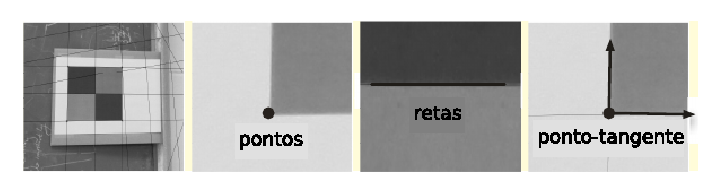
\includegraphics[width=\hsize]{astrom-objetos-geo}
\legend{Objetos utilizados para gerar equações na determinação dos parâmetros de $P$.}
\source{Kuang e \AA strom (2013).}
\label{fig.astrom-objetos-geo}
\end{figure}
\section*{Equações obtidas usando pontos.}

Dado um ponto 3D $\X$ e sua respectiva imagem em 2D $\x=(x,y,1)^\top$, a equação de projeção $\lambda\,\x=P\,\X$ nos fornece três equações. Mas, pela Subseção \ref{sec.ponto}, um ponto 2D tem apenas dois graus de liberdade apesar de suas três componentes, então dessas três equações apenas duas são linearmente independentes. Para eliminarmos o fator de escala $\lambda$ aplicamos o produto vetorial em ambos os lados da equação de projeção:
\begin{equation}\label{eq.astrom-pontos}
\begin{array}{rcl}
\lambda\,\x&=&P\,\X\\
\lambda\,[\x]_\times\x&=&[\x]_\times P\,\X\\
{\bf 0}&=&[\x]_\times P\,\X.
\end{array}
\end{equation}
\section*{Equações obtidas usando retas.} 

Uma reta 3D ${\bf L}$ pode ser representada usando um ponto $\X$ e uma direção ${\bf D}$, na forma ${\bf L}=\X+k\,{\bf D}$. Dadas a reta ${\bf L}$ e sua imagem $\lightrgb$ obtemos duas equações usando os dois pontos $\X$ e ${\bf D}$. Um ponto $\x$ pertence a uma reta $\lightrgb$ se $\lightrgb^\top\x=0$, e substituindo essa relação na equação de projeção \ref{eq.projecao} temos:
\begin{equation}\label{eq.astrom-retas}
\begin{array}{rcll}
\lightrgb^\top P\,\X&=&0&\text{se}\,\,\,k=0\\
\lightrgb^\top P(\X+k\,{\bf D})&=&0&\text{se}\,\,\,k\neq0.
\end{array}
\end{equation}  
\section*{Equações obtidas usando pontos-tangentes.}

É possível obter mais três equações se conhecemos o ponto $\X$, uma direção ${\bf D}$ através $\X$ bem como suas respectivas imagens $\x$ e ${\bf d}$. Com a correspondência $\X\leftrightarrow\x$ podemos usar a relação apresentada na Equaç\~ao \ref{eq.astrom-pontos} e conseguir duas equações. Para a terceira equação, usamos a reta definida pelos pontos na imagem, $\lightrgb=\x\times{\bf d}$, juntamente com as Equações \ref{eq.astrom-retas}, pois tomando a diferença entre tais equações e usando a reta $\lightrgb$ temos
\begin{equation}\label{eq.astrom-direcao}
\lightrgb^\top P\,{\bf D}=0.
\end{equation}  
Note que essas três equações são obtidas usando um ponto-tangente com uma direção apenas. Se usarmos ponto-tangente com mais direções, conseguimos uma equação a mais para cada direção, pois para cada ${\bf D}_i$ das $n$ direções, teremos $\lightrgb_i=\x\times{\bf d}_i$ e podemos formular as equações
\begin{equation}
[\x]_\times P\,\X={\bf 0}\quad\text{e}\quad\lightrgb_i^\top P\,{\bf D}_i=0\quad\text{para}\,\,i=1,...,n.
\end{equation}
Na tabela abaixo podemos verificar um resumo da quantidade de equações conseguidas para correspondências entre cada objeto geométrico.
\begin{center}
\begin{tabular}{|c|c|c|c|}
\hline 
{\bf ponto} & {\bf reta} & {\bf ponto com 1 tangente} & {\bf ponto com 2 tangentes} \\ 
\hline 
2 & 2 & 3 & 4 \\ 
\hline 
\end{tabular} 
\end{center}
\section*{Casos úteis.}

Com as quantidades de equações fornecidas por cada correspondência podemos formar várias combinações entre pontos, retas e ponto-tangentes para obtermos as sete equações necessárias para calcular os sete graus de liberdade de $P$. Vamos ver dois exemplos de problema mínimo.
\begin{itemize}
\item {\bf Dois pontos e um ponto-tangente (P2T1)}: com essa combinação temos três pontos e uma direção passando por um dos pontos, então podemos formar seis equações usando a Relação \ref{eq.astrom-pontos} e mais uma equação usando a Relação \ref{eq.astrom-direcao}. 

\item {\bf Um ponto-tangente com uma direção mais um ponto-tangente com duas direções (T1T2)}: temos uma reta passando por um dos pontos e duas retas passando pelo outro ponto, então podemos formar quatro equações usando \ref{eq.astrom-pontos} e mais três equações usando \ref{eq.astrom-direcao}.
\end{itemize} 

Podemos formar outros problemas mínimos conforme os apresentados aqui e vamos mostrar agora um caso supra-restringido, onde temos mais equações do que incógnitas a determinar.
\begin{itemize}
\item {\bf Quatro retas (P4L)}: Dadas quatro correspondências entre retas temos oito equações usando as Relações \ref{eq.astrom-retas}. Como precisamos de sete equações podemos usar uma delas para verificar a solução dada pelas demais.
\end{itemize}
\section*{Parametrização de $P$.}

Uma das ideias teóricas mais importantes do método e que a matriz de rotação da câmera é parametrizada com quaternions, pois desse modo produz sistemas de equações polinomiais relativamente fáceis de serem resolvidos. Utilizando quaternions, a matriz de rotação é dada por
\begin{equation*}
R=
\begin{bmatrix}
a^2+b^2-c^2-d^2&2bc-2ad&2ac+2bd\\
2ad+2bc&a^2-b^2+c^2-d^2&2cd-2ab\\
2bd-2ac&2ab+2cd&a^2-b^2-c^2+d^2
\end{bmatrix}
\end{equation*}
Se tratando de uma representação em coordenadas homogêneas podemos usar uma das variáveis para fixar a escala, assim tomando $a=1$ reduzimos o número de variáveis e facilitamos a solução do sistema de equações polinomiais.

O vetor de translação é parametrizado normalmente como ${\bf t}=(t_x,t_y,t_z)^\top$ e a matriz $[R|{\bf t}]$ se torna
\begin{equation*}
[R|{\bf t}]=
\begin{bmatrix}
a^2+b^2-c^2-d^2&2bc-2ad&2ac+2bd&t_x\\
2ad+2bc&a^2-b^2+c^2-d^2&2cd-2ab&t_y\\
2bd-2ac&2ab+2cd&a^2-b^2-c^2+d^2&t_z
\end{bmatrix}
\end{equation*}
Para completar a matriz $P$ basta aplicar, à esquerda de $[R|{\bf t}]$ a matriz de calibração $K$ conforme \ref{eq.astrom-K}.
\begin{equation*}
\begin{array}{rcl}
P&=&K\,[R|{\bf t}]\\\\
&=&
\begin{bmatrix}
1&0&0\\
0&1&0\\
0&0&w
\end{bmatrix}
\begin{bmatrix}
a^2+b^2-c^2-d^2&2bc-2ad&2ac+2bd&t_x\\
2ad+2bc&a^2-b^2+c^2-d^2&2cd-2ab&t_y\\
2bd-2ac&2ab+2cd&a^2-b^2-c^2+d^2&t_z
\end{bmatrix}\\\\
&=&
\begin{bmatrix}
a^2+b^2-c^2-d^2&2bc-2ad&2ac+2bd&t_x\\
2ad+2bc&a^2-b^2+c^2-d^2&2cd-2ab&t_y\\
w\,(2bd-2ac)&w\,(2ab+2cd)&w\,(a^2-b^2-c^2+d^2)&w\,t_z
\end{bmatrix}
\end{array}
\end{equation*} 
Substituindo $t'_z=w\,t_z$, temos que determinar as sete variáveis $\{b,c,d,t_x,t_y,t'_z,w\}$. Mas observe que as variáveis $\{t_x,t_y,t'_z\}$ são todas lineares usando as Relações \ref{eq.astrom-pontos}, \ref{eq.astrom-retas} e \ref{eq.astrom-direcao}, e portanto podem ser eliminadas do sistemas de equações restando apenas as quatro variáveis $\{b,c,d,w\}$. Depois de determinadas essas quatro variáveis, o vetor de translação pode ser recuperado por substituição. 
\section{Sistema de equações polinomiais}

Para resolver computacionalmente os sistemas de equações polinomiais decorrentes do emprego dos casos úteis na determinação de $P$, Kuang e \AA str\:om (2013) utilizam m\'etodos baseados em geometria algébrica. Primeiramente, utilizando a ferramenta {\it Macaulay2}, Grayson e Stillman (1993-2002), é verificada a existência de 20 soluções para o caso mínimo (P2T1). Para sistemas com pouca quantidade de variáveis, usar apenas o método das bases de Gr\"obner pode ser rápido e numericamente estável, mas aqui é empregado o método exposto em Byr\"od et al. (2009), que consiste basicamente em extrair a base linear a partir das bases de Gr\"obner e empregar a matriz de ação, da qual as soluções podem ser obtidas pela decomposição em autovalores. No apêndice \ref{sec.geo-algebrica} é fornecido um resumo sobre a teoria básica de geometria algébrica, bem como exemplos da utilização do método das bases de Gr\"obner e da matriz de ação para resolver sistemas computacionalmente.

\newpage
\chapter{Geometria trifocal}\label{sec.geo-tri}
Assim como num sistema com duas imagens, podemos extrair informações sobre o cenário em 3D através da correspondência entre pontos, retas, tangentes e segmentos de curvas com três  ou mais imagens. No entanto, grande parte das pesquisas em visão computacional não tem utilizado a geometria trifocal em problemas de reconstrução 3D e transferência de pontos de uma imagem para outra. Menor ainda é a utilização da geometria diferencial para abordar esses problemas para curvas gerais, tais como cristas de ondas. Um dos nossos objetivos é fazer um levantamento das características e conceitos encontrados num sistema trifocal em comparação com a geometria epipolar, e relatar alguns dos benefícios conseguidos através da inclusão de uma terceira imagem.
\begin{figure}[htb!]{\textwidth}
\caption{Plataforma espanhola.}
\subfloat{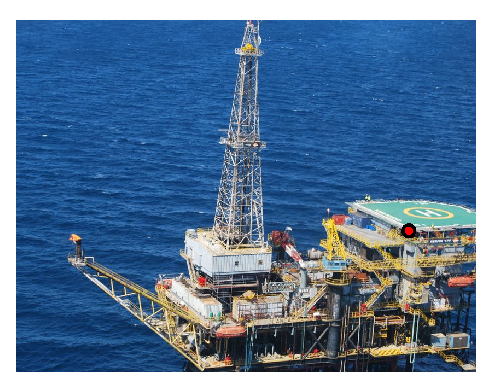
\includegraphics[scale=.67]{plataforma-1}}\hfill
\subfloat{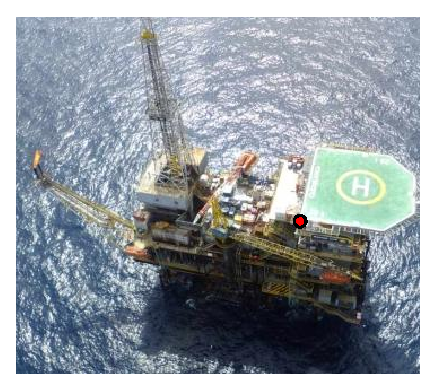
\includegraphics[scale=.67]{plat-2}}\hfill
\subfloat{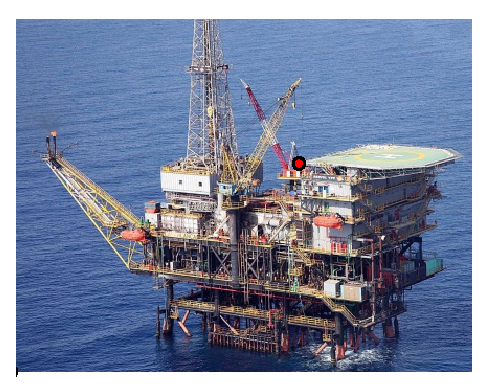
\includegraphics[scale=.67]{plat-3}}\hfill
\legend{Três imagens da plataforma petrolífera espanhola Casablanca. Exemplo de três pontos correspondentes em vermelho representando um canto do heliporto.}
\source{http://www.repsol.com/}
\end{figure}
\section{O Problema}
Considere um cenário em 3D com três imagens em 2D desse cenário conforme a Figura \ref{fig.trifocal-frente}, onde podemos visualizar as três imagens $\x$, $\x'$ e $\x''$ de um ponto 3D $\X$ (dois sinais de apóstrofo indicam o objeto pertencente à terceira câmera) e os pontos correpondentes $\x\leftrightarrow\x'\leftrightarrow\x''$ são previamente conhecidos. O desafio da reconstrução 3D é determinar, a partir das correspondências nas imagens, as matrizes das câmeras $P$, $P'$ e $P''$ que realizam as projeções $\x=P\,\X$, $\x'=P'\X$ e $\x''=P''\X$ em cada imagem, bem como a determinação do ponto $\X$. Nesse trabalho está sendo dada prioridade à determinação das matrizes das câmeras, por ser um dos maiores problemas atuais em visão computacional e que torna-se primordial no caso da correspond\^encia entre curvas Fabbri e Kimia (2011).

É mais comum a utilização da geometria epipolar bifocal para problemas de reconstrução 3D, fazendo a extração das câmeras usando a geometria epipolar e aplicando um algoritmo para determinação do ponto 3D a partir da triangulação $(\x,\x',\X)$. Mas quando aumentamos para três a quantidade de imagens, aumentam-se também as possibilidades de degenerações (que depende  da posição do ponto 3D $\X$) se continuarmos utilizando as ferramentas da geometria epipolar a cada par de imagens. Mostraremos que alguns casos de degenerações podem ser removidos usando a teoria da geometria trifocal.


Vamos aplicar o procedimento desenvolvido por Faugeras et al. (2001) que consiste em utilizar a geometria epipolar bifocal num problema de transferência de pontos num sistema trifocal, avaliar as deficiências dessa abordagem e em seguida mostrar como a geometria trifocal pode erradicar algumas dessas deficiências. 
\begin{figure}[!htb]{.9\textwidth}
\caption{Geometria trifocal.}
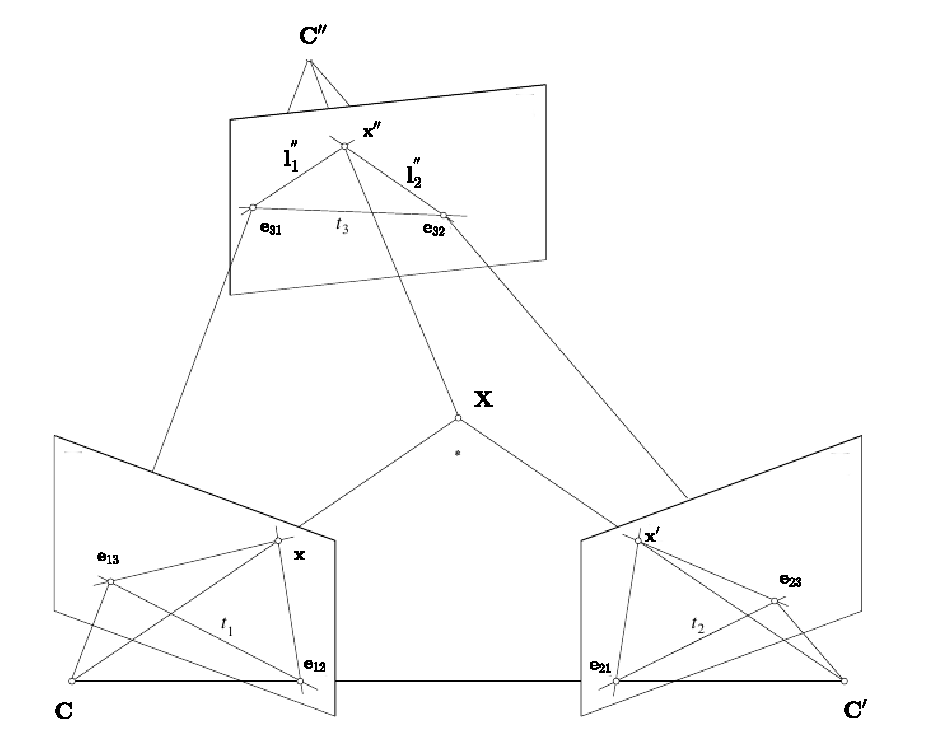
\includegraphics[width=\hsize]{trifocal-frente-frente}
%\legend{O plano trifocal juntamente com os três planos epipolares. A transferência epipolar falha em alguns casos.}
\source{Adaptado, Forsyth e Ponce (2003).}
\label{fig.trifocal-frente}
\end{figure}
O plano definido pelos pontos $\C, \C' \,\,\text{e}\,\, \X$ forma o plano epipolar para as câmeras 1 e 2. Analogamente, temos o plano epipolar para as câmeras 1 e 3 e para as câmeras 2 e 3. A interseção de cada plano epipolar com os planos das imagens geram as retas epipolares. Por exemplo, a reta  epipolar $\lightrgb''_1$ definida pelos pontos $\e_{31}$ e $\x''$ na terceira imagem, é a reta epipolar com relação ao ponto $\x$ na primeira imagem. Ou seja, $\lightrgb''_1$ é a imagem, na câmera 3, da reta retroprojetada por $\x$ através do centro de projeção $\C$ na câmera 1. Essa reta é definida por $\lightrgb''_1=F_{31}\,\x$ ou $\lightrgb''_1=\e_{31}\times\x''$, onde $F_{ij}$ é a matriz fundamental para as câmeras $i$ e $j$ tomando como base a câmera $j$. O plano formado pelos centros de projeção $\C, \C' \,\,\text{e}\,\, \C''$ é chamado {\it plano trifocal} e as interseções desse plano com os planos das imagens geram as {\it retas trifocais} denotadas por ${\bf t}_i$.

\section{Transferência epipolar}\label{sec.trans-epipolar}
Supondo que temos os pontos correspondentes $\x\leftrightarrow\x'$ para as câmeras 1 e 2, bem como as matrizes fundamentais para os três planos epipolares da Figura \ref{fig.trifocal-frente}, $F_{21}$, $F_{31}$ e $F_{32}$, desejamos determinar as coordenadas do ponto $\x''$ no plano de imagem da câmera 3. Como vimos, os pontos $\x$, $\x'$ e $\x''$ são imagens de um mesmo ponto 3D $\X$, e por isso $\x''$ é um ponto correspondente ao ponto $\x$ e, portanto, $\x''\in\lightrgb''_1$, onde $\lightrgb''_1=F_{31}\x$ é a reta epipolar para as câmeras 1 e 3. Por um argumento similar, constatamos que $\x''$ é correspondente ao ponto $\x'$ e por isso $\x''\in\lightrgb''_2=F_{32}\x'$. Como temos os pontos e as matrizes fundamentais, podemos calcular as retas epipolares na terceira imagem. O ponto $\x''$ será calculado como a interseção entre essas duas retas:
\begin{equation}
\begin{array}{rcl}
\x''&=&\lightrgb''_1\times\lightrgb''_2\\
\x''&=&F_{31}\x\times F_{32}\x'.
\end{array}
\end{equation}
Esse metodo é chamado de {\it transferência epipolar} e não podemos determinar $\x''$ nos seguintes casos:
\begin{itemize}
\item acompanhando ainda pela Figura \ref{fig.trifocal-frente}, observa-se que se o ponto 3D $\X$ pertence à reta base definida por $\C$ e $\C''$, então a projeção desse ponto pela câmera 1 será $\x=P\,\X=\e_{13}$, já que $\X$ está alinhado com $\C''$ e $\e_{13}=P\,\C''$. Sendo $\x=\e_{13}$ temos que, pela Subseção \ref{sec.propriedades-F} $F_{31}\e_{13}={\bf 0}$, e a reta epipolar $\lightrgb''_1={\bf 0}$. Geometricamente, não podemos determinar um plano epipolar para as câmeras 1 e 3;
\item analogamente ao caso anterior, se $\X$ pertence à reta base definida por $\C'$ e $\C''$, não podemos definir o plano epipolar para as câmeras 2 e 3;\\
\end{itemize}

Já que o ponto procurado $\x''$ é calculado como interseção das duas retas epipolares $\lightrgb''_1$ e $\lightrgb''_2$, o procedimento de tranferência falha em mais dois casos quando essas retas são iguais ou muito próximas.

\begin{itemize}
\item repare que se os centros de projeção não estão alinhados então os epipolos $\e_{31}$ e $\e_{32}$ são diferentes. As retas epipolares $\lightrgb''_1$ e $\lightrgb''_2$ são iguais se $\e_{31}\in\lightrgb''_2$ e $\e_{32}\in\lightrgb''_1$. Geometricamente, isso significa que o ponto $\X$ está alojado no plano trifocal e $\x''\in{\bf t}_3$.

\item se os centros de projeção estão alinhados então os epipolos $\e_{31}$ e $\e_{32}$ são iguais, e daí $\lightrgb''_1=\lightrgb''_2$. Geometricamente, temos infinitos planos passando pela reta definida por $\C$, $\C'$ e $\C''$, e o ponto $\x''$ será indeterminado para qualquer ponto $\X$ no espaço 3D.
\end{itemize}

Todos os casos se resumem ao fato de o ponto $\X$ estar alojado no plano trifocal, pois desse jeito os planos epipolares coincidem com o plano trifocal. Mais ainda, a acurácia do ponto $\x''$ fica bastante prejudicada se $\X$ está próximo do plano trifocal, pois as retas epipolares se tornam menos transversas. 

Mostramos a determinação do ponto $\x''$ especificamente, mas esse desenvolvimento através da transferência epipolar é análogo para a predição de $\x$ ou $\x'$. Quase todos os casos de degeneração são resolvidos através da introdução de uma outra ferramenta algébrica, o {\it tensor trifocal}.

\section{O tensor trifocal e as relações de incidência}\label{sec.tensor-tri-rela-inci}

Para a derivação do tensor trifocal usaremos a correspondência entre retas $\lightrgb\leftrightarrow\lightrgb'\leftrightarrow\lightrgb''$ ao longo de três imagens, onde todas essas retas são imagens de uma mesma reta $\bf L$ no espaço 3D. Esse é o procedimento padrão desenvolvido originalmente por Spetsakis e Aloimonos (1990) e reproduzido, por exemplo, por Faugeras et al. (2001) e Forsyth e Ponce (2003). A abordagem algébrica aqui utilizada pode ser encontrada em Hartley e Zisserman (2004).

Suponha que temos três imagens em 2D $\lightrgb$, $\lightrgb'$ e $\lightrgb''$  de uma reta ${\bf L}$ em 3D, conforme a Figura \ref{fig.abord-geo-tri}. Pela Subseção \ref{sec.proj.retas}, essas três retas nas imagens retroprojetam planos que, pela própria construção, devem se interceptar em ${\bf L}$. Esta imposição geométrica gera uma restrição algébrica para as três retas correspondentes, já que em geral três planos no espaço não se interceptam numa única reta. Pela Subseção \ref{sec.cameras-canonicas}, através de uma transformação projetiva podemos utilizar o conjunto de matrizes canônicas para as câmeras $P=[I|{\bf 0}]$, $P'=[A|{\bf a}_4]$ e $P''=[B|{\bf b}_4]$, onde $A$ e $B$ são matrizes $3\times3$ e os vetores ${\bf a}_i$ e ${\bf b}_i$ representam a $i$-ésima coluna das câmeras $P'$ e $P''$ respectivamente, para $i=1,2,3 \,\,\text{e}\,\, 4$.

Observa-se que tomando $P=[I|{\bf 0}]$ estamos considerando o centro da câmera 1 como a origem de coordenadas do espaço 3D, e assim as coordenadas do centro da câmera 1 são $\C=(0,0,0,1)^\top$. Os epipolos na segunda e terceira imagens em relação à câmera 1 são, respectivamente, dados pela projeção $\e'=P'\C$ e $\e''=P''\C$, e assim temos que $\e'={\bf a}_4$ e $\e''={\bf b}_4$ (já que não vamos mais nos referir aos demais epipolos de um sistema trifocal, usaremos a notação simplificada $\e'$ e $\e''$). Como retas retroprojetam planos, esses planos são dados, de acordo com a Subseção \ref{sec.proj.retas}, por
\begin{equation*}
\begin{array}{rcl}
\pi&=&P^\top\lightrgb\\
\pi&=&
\begin{pmatrix}
\lightrgb\\
0
\end{pmatrix}
\end{array},\qquad
\begin{array}{rcl}
\pi'&=&P'^\top\lightrgb'\\
\pi'&=&
\begin{pmatrix}
A^\top\lightrgb'\\
{\bf a}^\top_4\lightrgb'
\end{pmatrix}
\end{array}\quad\text{e}\quad
\begin{array}{rcl}
\pi''&=&P''^\top\lightrgb''\\
\pi''&=&
\begin{pmatrix}
B^\top\lightrgb''\\
{\bf b}^\top_4\lightrgb''
\end{pmatrix}
\end{array}.
\end{equation*}
Como estamos supondo que essas três retas são imagens de uma única reta no espaço, temos que esses três planos devem se interceptar em ${\bf L}$, e essa restrição geométrica pode ser expressa algebricamente pelo fato de que a matriz formada pelos vetores dos três planos $M=[\pi \,\,\pi'\,\,\pi'']$ deve ter posto dois. De fato, um ponto $\X\in{\bf L}$ pode ser escrito como combinação linear de outros dois pontos pertencentes a ${\bf L}$ que sejam linearmente independentes, digamos $\X=\lambda_1\X_1+\lambda_2\X_2$, com $\lambda_i$ escalares. Como $\X$ pertence a cada um dos planos, temos que $\bpi^\top\X=0$, $\bpi'^\top\X=0$ e $\bpi''^\top\X=0$, e daí $M^\top\X={\bf 0}$. Encarando $M^\top$ como um operador linear, desde que $\X=\lambda_1\X_1+\lambda_2\X_2$, temos que o núcleo de $M^\top$ tem dimensão dois, e como $M^\top$ tem quatro colunas o domínio tem dimensão quatro. 

Pelo teorema do núcleo e imagem de uma transformação linear, a dimensão do domínio é a soma da dimensão do núcleo com a dimensão da imagem, e daí a dimensão da imagem é dois. A dimensão da imagem é o posto do operador linear $M^\top$, que é igual ao posto de $M$.
\begin{figure}[!htb]{12cm}
\caption{Tr\^es imagens de uma reta.}
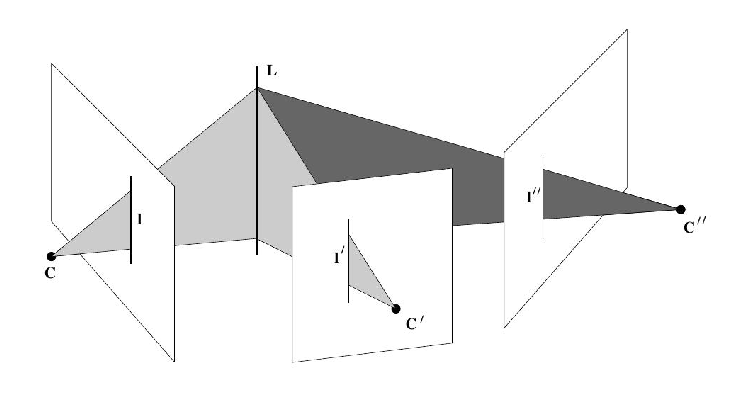
\includegraphics[width=\hsize]{abord-geo-tri}
\legend{O desenvolvimento algébrico do tensor trifocal realizado a partir das três imagens de uma reta no espaço 3D.}
\source{Hartley e Zisserman (2004).}
\label{fig.abord-geo-tri}
\end{figure}
Considerando $\alpha$, $\beta$ e $k$ escalares, o posto dois de $M$ pode ser interpretado com uma dependência linear entre suas colunas, e como
\begin{equation*}
M=
\begin{bmatrix}
\lightrgb&A^\top\lightrgb'&B^\top\lightrgb''\\
0&{\bf a}^\top_4\lightrgb'&
{\bf b}^\top_4\lightrgb''
\end{bmatrix},
\end{equation*}
podemos definir o sistema:
\begin{equation}\label{eq.sistema-tri}
\begin{pmatrix}
\lightrgb\\
0
\end{pmatrix}
=
\alpha
\begin{pmatrix}
A^\top\lightrgb'\\
{\bf a}^\top_4\lightrgb'
\end{pmatrix}
+\beta
\begin{pmatrix}
B^\top\lightrgb''\\
{\bf b}^\top_4\lightrgb''
\end{pmatrix}.
\end{equation}
Pela quarta equação do sistema \ref{eq.sistema-tri} temos
\begin{equation*}
\alpha=k\,{\bf b}^\top_4\lightrgb''\quad\text{e}\quad\beta=-k\,{\bf a}^\top_4\lightrgb'\quad\Rightarrow\quad0=\alpha\,{\bf a}^\top_4\lightrgb'+\beta\,{\bf b}^\top_4\lightrgb''.
\end{equation*}
Substituindo os valores de $\alpha$ e $\beta$ nas três primeiras equações do sistema \ref{eq.sistema-tri} e desconsiderando o fator de escala $k$, temos
\begin{equation*}
\begin{array}{rcl}
\lightrgb&=&\alpha\,A^\top\lightrgb'+\beta\,B^\top\lightrgb''\\
\lightrgb&=&({\bf b}^\top_4\lightrgb'')A^\top\lightrgb'-({\bf a}^\top_4\lightrgb')B^\top\lightrgb''\\
\lightrgb&=&(\lightrgb''^\top{\bf b}_4)A^\top\lightrgb'-(\lightrgb'^\top{\bf a}_4)B^\top\lightrgb''.
\end{array}
\end{equation*}
A $i$-ésima coordenada de $\lightrgb$ pode ser dada por
\begin{equation*}
\begin{array}{rcl}
l_i&=&\lightrgb''^\top({\bf b}_4{\bf a}^\top_i)\lightrgb'-\lightrgb'^\top({\bf a}_4{\bf b}_i^\top)\lightrgb''\\
l_i&=&\lightrgb'^\top({\bf a}_i{\bf b}^\top_4)\lightrgb''-\lightrgb'^\top({\bf a}_4{\bf b}_i^\top)\lightrgb''\\
l_i&=&\lightrgb'^\top({\bf a}_i{\bf b}^\top_4-{\bf a}_4{\bf b}_i^\top)\lightrgb''\\
l_i&=&\lightrgb'^\top \mbox{T}_i\lightrgb'',
\end{array}
\end{equation*}
onde definimos $\mbox{T}_i={\bf a}_i{\bf b}^\top_4-{\bf a}_4{\bf b}_i^\top$. 
O conjunto das três matrizes $\left\{\mbox{T}_1,\mbox{T}_2,\mbox{T}_3\right\}$ é denominado {\it tensor trifocal} e a reta $\lightrgb$ é dada por
\begin{equation}\label{eq.tres-retas}
\lightrgb=
\begin{pmatrix}
\lightrgb'^\top \mbox{T}_1\lightrgb''\\
\lightrgb'^\top \mbox{T}_2\lightrgb''\\
\lightrgb'^\top \mbox{T}_3\lightrgb''
\end{pmatrix}.
\end{equation}

\subsection{Homografia induzida por um plano}\label{sec.homo-plano-tri}
Vimos na subseção anterior que podemos determinar o tensor trifocal através da relação entre três retas correspondentes, mas existem mais quatro relações entre retas e pontos  correspondentes envolvendo o tensor trifocal. Para derivarmos essas outras relações e voltarmos ao problema da transferência de pontos, precisamos definir a homografia entre a primeira e terceira imagens induzida por um plano $\bpi'$, retroprojetado por uma reta $\lightrgb'$ na segunda imagem, conforme a Figura \ref{fig.transfer-retas}.
\begin{figure}[!htb]{12cm}
\caption{Homografia planar e o tensor trifocal.}
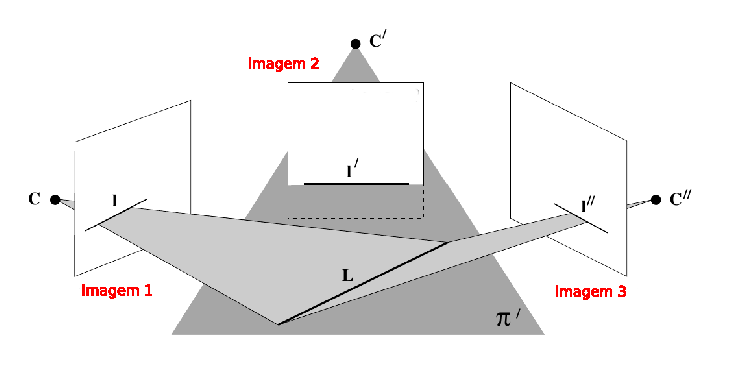
\includegraphics[scale=1]{transfer-retas}
\legend{O plano $\bpi'$ retroprojetado por $\lightrgb'$ induz uma homografia que relaciona $\lightrgb$ com $\lightrgb''$.}
\source{Adaptado, Hartley e Zisserman (2004).}
\label{fig.transfer-retas}
\end{figure}
As homografias entre pontos e retas em dois planos são dadas, respectivamente, por $\x''=H\,\x$ e $\lightrgb''=H^{-\top}\lightrgb$ (Subseção \ref{sec.trans-proj-H}). Invertendo $H^{-\top}$ temos que $\lightrgb=H^\top\lightrgb''$. Como temos três retas correspondentes que satizfazem a Relação \ref{eq.tres-retas}, podemos comparar essa relação com $\lightrgb=H^\top\lightrgb''$ e deduzir que $H=[\mbox{T}_1^\top\lightrgb',\mbox{T}_2^\top\lightrgb',\mbox{T}_3^\top\lightrgb']$, pois
\begin{equation*}
\lightrgb=
\begin{pmatrix}
\lightrgb'^\top \mbox{T}_1\lightrgb''\\
\lightrgb'^\top \mbox{T}_2\lightrgb''\\
\lightrgb'^\top \mbox{T}_3\lightrgb''
\end{pmatrix}=
\begin{pmatrix}
(\mbox{T}_1^\top\lightrgb')^\top\lightrgb''\\
(\mbox{T}_2^\top\lightrgb')^\top\lightrgb''\\
(\mbox{T}_3^\top\lightrgb')^\top\lightrgb''
\end{pmatrix}=
\begin{pmatrix}
{\bf h}_1^\top\lightrgb''\\
{\bf h}_2^\top\lightrgb''\\
{\bf h}_3^\top\lightrgb''
\end{pmatrix}=
\begin{bmatrix}
{\bf h}_1^\top\\
{\bf h}_2^\top\\
{\bf h}_3^\top
\end{bmatrix}\,\lightrgb''=
H^\top\lightrgb'',
\end{equation*}
onde tomamos ${\bf h}_i=\mbox{T}_i^\top\lightrgb'$.
A homografia deduzida acima (denotada por $H_{13}$) representa a transformação de um ponto da primeira imagem para a terceira através de uma reta na segunda imagem, $\x''=H_{13}\x$. Analogamente, podemos deduzir a homografia da primeira imagem para a segunda através de uma reta na terceira imagem, $\x'=H_{12}\x$.

\subsection{Relações de incidência entre pontos e retas}\label{sec.rela-incidi-tri}
Uma das relações de incidência já foi deduzida anteriormente, chamada reta-reta-reta, e agora vamos deduzir mais quatro relações. Supondo ainda $\lightrgb$, $\lightrgb'$ e $\lightrgb''$ três imagens de uma reta ${\bf L}$, sabemos que um ponto $\x$ pertence à uma reta $\lightrgb$ na câmera 1 se $\x^\top\lightrgb=0$, onde a multiplicação matricial pode ser escrita sob a notação de somatório como $\sum_{i=1}^{3}x^il_i=0$. O índice contravariante em $x$ é uma convenção para facilitar o algebrismo na notação padrão de tensor trifocal. Essa convensão se deve ao fato de o tensor trifocal possuir três índices e não apenas dois como ocorre com as matrizes. A Equação \ref{eq.tres-retas} pode ser dada como $\lightrgb'^\top \mbox{T}_i\lightrgb''
=l_i$ para $i=1,2,3$, e usando o somatório temos que
\begin{equation*}
\begin{array}{rcl}
\lightrgb'^\top \mbox{T}_i\lightrgb''
&=&l_i\\
\sum_{i=1}^3 x^i(\lightrgb'^\top \mbox{T}_i\lightrgb'')&=&\sum_{i=1}^3 x^il_i\\
\lightrgb'^\top(\sum_{i=1}^3 x^i\mbox{T}_i)\lightrgb''&=&0.
\end{array}
\end{equation*}
Desta forma, temos a segunda relação de incidência chamada ponto-reta-reta, para um ponto $\x$ na primeira imagem e as retas $\lightrgb'$ e $\lightrgb''$ na segunda e terceira imagens respectivamente. 

Pela Subseção \ref{sec.proj.retas} sabemos da existência de um ponto $\X\in{\bf L}$ que projeta $\x\in\lightrgb$ na primeira imagem e projeta a outros dois pontos $\x'\in\lightrgb'$ e $\x''\in\lightrgb''$, ou seja, temos a correspondência $\x\leftrightarrow\x'\leftrightarrow\x''$. Assim, podemos deduzir as relações para 
pontos na segunda e terceira imagens utilizando a homografia induzida por plano, e vamos tratar da terceira relação de incidência, o caso ponto-reta-ponto. Usando o resultado da Subseção \ref{sec.homo-plano-tri} temos que 
\begin{equation*}
\begin{array}{rcl}
\x''&=&H_{13}\x\\
&=&[\mbox{T}_1^\top\lightrgb',\mbox{T}_2^\top\lightrgb',\mbox{T}_3^\top\lightrgb']\x\\
&=&
\begin{pmatrix}
x_1\mbox{T}_1^\top\lightrgb'+x_2\mbox{T}_2^\top\lightrgb'+x_3\mbox{T}_3^\top\lightrgb'
\end{pmatrix}\\
&=&(\sum_{i=1}^3 x^i\mbox{T}_i^\top)\,\lightrgb'
\end{array}
\end{equation*}
Como estamos expressando os vetores em coordenadas homogêneas, essas equações são invariantes para a aplicação de um fator de escala. De qualquer maneira, podemos eliminar o problema das diferenças de escala aplicando a transposição seguida do produto vetorial à direita em ambos os lados da equação
\begin{equation}\label{eq.ponto-reta-ponto}
\begin{array}{rcl}
\x''&=&(\sum_{i=1}^3 x^i\mbox{T}_i^\top)\,\lightrgb'\\
\x''^\top&=&\lightrgb'^\top(\sum_{i=1}^3 x^i\mbox{T}_i)\\
\x''^\top[\x'']_\times&=&\lightrgb'^\top(\sum_{i=1}^3 x^i\mbox{T}_i)[\x'']_\times\\
{\bf 0}^\top&=&\lightrgb'^\top(\sum_{i=1}^3 x^i\mbox{T}_i)[\x'']_\times.
\end{array}
\end{equation}
O quarto caso, ponto-ponto-reta, é análogo ao apresentado aqui substituindo $\x''$ por $\x'$, e usando a homografia induzida pelo plano retroprojetado por $\lightrgb''$, $\x'=H_{12}\x$.

Por último, temos a relação de incidência para três pontos. 
Observe que a reta $\lightrgb'$ na Relação \ref{eq.ponto-reta-ponto} pode ser definida como $\lightrgb'=\x'\times \y'=[\x']_\times \y'$, já que $\x'\in\lightrgb'$ e $\y'$ é um ponto qualquer no plano da segunda imagem. Substituindo $\lightrgb'$, a Relação \ref{eq.ponto-reta-ponto} se torna 
\begin{equation*}
\y'^\top[\x']_\times(\sum_{i=1}^3 x^i\mbox{T}_i)[\x'']_\times={\bf 0}^\top,
\end{equation*}
mas observa-se que tal relação é válida para qualquer reta $\lightrgb'$ que seja imagem de ${\bf L}$, e portanto não depende da escolha do ponto $\y'$ que pode ser descartado. A relação ponto-ponto-ponto é
\begin{equation*}
[\x']_\times(\sum_{i=1}^3 x^i\mbox{T}_i)[\x'']_\times=0_{3\times3}.
\end{equation*}
Cabe resaltar que apenas satisfazer qualquer das relações de incidência não garante a incidência no espaço 3D, ou seja, o tensor trifocal obtido pode não ter consistência com a geometria trifocal de abordagem do problema.

\subsection{Relação de incidência para retas epipolares}\label{sec.rela-reta-epipolar-tri}
Suponha que os planos retroprojetados por $\lightrgb$ e $\lightrgb'$ sejam coincidentes e que o ponto 3D $\X$ pertença a esse plano denotado por $\bpi'$, de acordo com a Figura \ref{fig.plano-epipolar-tri}. Neste caso, $\bpi'$ é o plano epipolar para as câmeras 1 e 2, e a reta retroprojetada por $\x$, imagem de $\X\in{\bf L}$, está inteiramente contida em $\bpi'$. Como dois planos não coincidentes sempre definem uma reta, o plano retroprojetado por $\lightrgb''$ intercepta o plano $\bpi'$ em ${\bf L}$. Já que a reta retroprojetada por $\x$ está inteiramente contida em $\bpi'$, essa reta deverá interceptar a reta ${\bf L}$ no ponto $\X$. Desta forma, pela Subseção \ref{sec.rela-incidi-tri}, temos a correspondência $\x\leftrightarrow\lightrgb'\leftrightarrow\lightrgb''$ que satisfaz a relação
\begin{equation*}
\lightrgb'^\top(\sum_{i=1}^3 x^i\mbox{T}_i)\lightrgb''=0.
\end{equation*}
Observe que, como dois planos sempre definem uma reta, a incidência não depende da escolha do plano retroprojetado pela câmera 3, ou seja, essa incidência vai ocorrer qualquer que seja a reta $\lightrgb''$. Consequentemente, a relação anterior não depende de $\lightrgb''$, e pode ser reduzida a 
\begin{equation}\label{eq.rela-incide-epipolar}
\lightrgb'^\top(\sum_{i=1}^3 x^i\mbox{T}_i)={\bf 0}^\top\quad\text{ou}\quad(\sum_{i=1}^3 x^i\mbox{T}_i)\lightrgb''={\bf 0}.
\end{equation}
A argumentação é análoga considerando o plano epipolar definido pelas retas $\lightrgb$ e $\lightrgb''$, e neste caso a relação será independente da posição da reta $\lightrgb'$. 
\begin{figure}[!htb]{12cm}
\caption{Transfer\^encias com retas epipolares.}
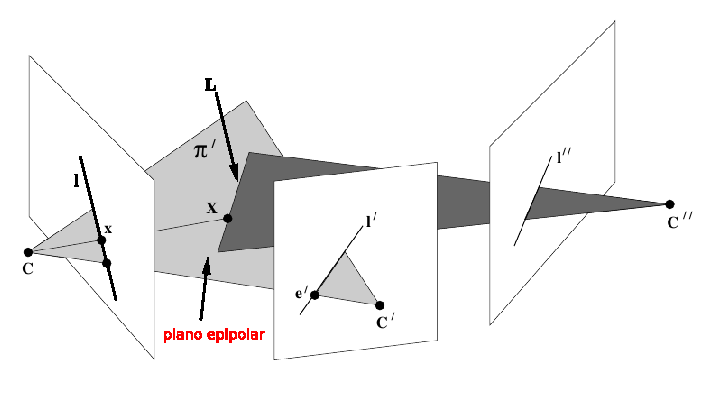
\includegraphics[width=\hsize]{plano-epipolar-tri}
\legend{Quando ${\bf L}$ pertence a um plano epipolar definido para duas imagens, a relação de incidência $\x\leftrightarrow\lightrgb'\leftrightarrow\lightrgb''$ não depende da reta numa terceira imagem.}
\source{Adaptado, Hartley e Zisserman (2004).}
\label{fig.plano-epipolar-tri}
\end{figure}
Pelas Relações \ref{eq.rela-incide-epipolar} notamos que é possível calcular as retas epipolares como o espaço nulo da matriz $\sum_{i=1}^3 x^i \mbox{T}_i$. Variando o ponto $\x$ é possível obter várias retas epipolares, e todas passam pelo mesmo epipolo. Assim, podemos calcular os epipolos $\e'$ e $\e''$ como interseção dessas retas. Tal resultado será importante na abordagem sobre reconstrução 3D por ocasião da extração das matrizes das câmeras a partir do tensor trifocal.

\section{Transferências usando o tensor trifocal}

\subsection{Transferência de pontos}
A primeira vantagem no uso do tensor trifocal é que, dos casos de degeneração apresentados na Subseção \ref{sec.trans-epipolar}, apenas um deles não pode ser resolvido pelo uso do tensor, como veremos a seguir. 

Considere novamente que se deseja, dada a correspondência entre pontos nas duas primeiras imagens $\x\leftrightarrow\x'$, determinar as coordenadas do ponto correspondente na terceira imagem, $\x''$. Escolhendo uma reta $\lightrgb'$ passando por $\x'$ na segunda imagem e de posse do tensor trifocal, podemos utilizar a relação de incidência 
\begin{equation}\label{eq.ponto-reta-ponto-isolada}
\x''=(\sum_{i=1}^3 x^i\mbox{T}_i^\top)\,\lightrgb'
\end{equation} 
deduzida na Subseção \ref{sec.rela-incidi-tri}
para computar diretamente $\x''$. Devemos apenas ter um pouco de cuidado na escoha da reta $\lightrgb'$, pois no caso de ser a reta epipolar correspondente a $\x$ temos, pela Subseção \ref{sec.rela-reta-epipolar-tri}, que $(\sum_{i=1}^3 x^i\mbox{T}_i^\top)\,\lightrgb'={\bf 0}$, e o ponto $\x''$ não pode ser determinado. Uma das formas de resolver o problema seria escolher duas ou três retas passando por $\x'$, computar o ponto $\x''$ e escolher aquele que apresenta a maior norma. Outra opção, caso tenha extraído a matriz fundamental $F_{21}$ para as câmeras 1 e 2, é calcular a reta epipolar $\lightrgb'_{\e}=F_{21}\x$ e escolher $\lightrgb'$ que seja perpendicular a $\lightrgb'_{\e}$, ou seja, $\lightrgb'^\top\lightrgb'_{\e}=0$. 

Considere, pela Figura \ref{fig.trifocal-frente}, o caso onde o ponto $\X$ está alojado na reta base definida por $\C$ e $\C'$. Nessa posição, a imagem de $\X$ na câmera 2 é o epipolo $\e_{21}=\x'$. Para escolha de qualquer reta que passe por $\x'$ para aplicarmos a Relação \ref{eq.ponto-reta-ponto-isolada}, estaremos escolhendo uma reta epipolar, e como vimos anteriormente, não poderemos definir a posição do ponto $\x''$. Tal reta base é o único lugar que $\X$ pode se alojar no plano trifocal que não permite que o ponto $\x''$ seja calculado usando o tensor trifocal, em contraste com a transferência epipolar que se degenera para qualquer $\X$ no plano trifocal. Observe pela Figura \ref{fig.X-plano-trifocal} que, desde que a reta ${\bf L}$ não pertença ao plano trifocal, não há motivos para a degeneração da transferência usando o tensor trifocal à medida que variamos a posição de $\X$ em ${\bf L}$. 
\begin{figure}[!htb]{12cm}
\caption{Reduç\~ao de degeneraç\~oes.}
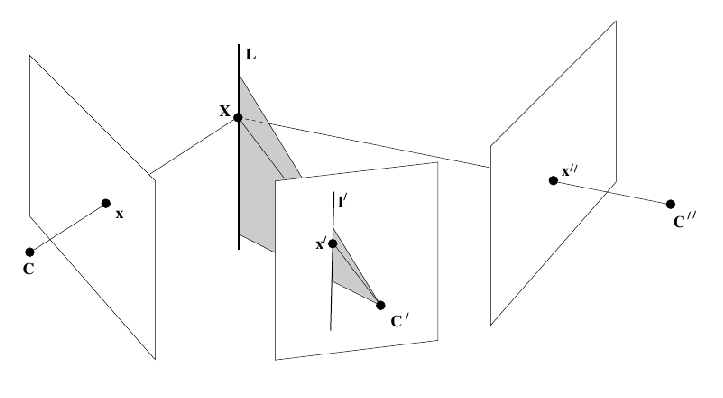
\includegraphics[scale=1]{X-plano-trifocal}
\legend{Desde de que ${\bf L}$ não pertença ao plano trifocal, não há motivos para degenerações à medida que variamos $\X$ em ${\bf L}$.}
\source{Hartley e Zisserman (2004).}
\label{fig.X-plano-trifocal}
\end{figure}
No caso onde os centros das câmeras estão alinhados, não poderemos determinar a posição de $\x''$ caso $\X$ esteja em quaisquer das três retas base, já que assim essas três retas são uma reta só. Lembramos que a transferência epipolar falha para centros de projeção alinhados qualquer que seja a posição de $\X$.  
\subsection{Transferência de retas}
Podemos realizar a transferência de retas utilizando a relação
\begin{equation*}
\lightrgb=
\begin{pmatrix}
\lightrgb'^\top \mbox{T}_1\lightrgb''\\
\lightrgb'^\top \mbox{T}_2\lightrgb''\\
\lightrgb'^\top \mbox{T}_3\lightrgb''
\end{pmatrix},
\end{equation*}
que dá uma maneira explícita de calcularmos a reta na primeira imagem dadas as retas nas câmeras 2 e 3. Mas podemos calcular retas em quaisquer das três imagens dadas as outras duas, aplicando o produto vetorial por $\lightrgb$ em ambos os lados da equação
\begin{equation*}
\begin{array}{rcl}
\lightrgb\times\lightrgb&=&\lightrgb\times
\begin{pmatrix}
\lightrgb'^\top \mbox{T}_1\lightrgb''\\
\lightrgb'^\top \mbox{T}_2\lightrgb''\\
\lightrgb'^\top \mbox{T}_3\lightrgb''
\end{pmatrix}\\
{\bf 0}&=&\lightrgb\times
\begin{pmatrix}
\lightrgb'^\top \mbox{T}_1\lightrgb''\\
\lightrgb'^\top \mbox{T}_2\lightrgb''\\
\lightrgb'^\top \mbox{T}_3\lightrgb''
\end{pmatrix}.\\
\end{array}
\end{equation*}
O sistema fornece três equações, sendo duas independentes, para determinar os dois graus de liberdade da reta procurada. Outra vantagem no uso de tensor trifocal é que retas explícitas não podem ser determinadas usando apenas matrizes fundamentais.

Repare, pela Figura \ref{fig.plano-epipolar-tri}, que se as retas $\lightrgb$ e $\lightrgb'$ retroprojetam o mesmo plano, então não teremos uma única reta definida em 3D que possa ser projetada na terceira imagem, e essas duas retas são retas epipolares correspondentes. Similarmente, não podemos determinar a reta na segunda imagem caso as retas na primeira e terceira imagens sejam retas epipolares correspondentes. Em posições gerais, não há motivo para a geometria epipolar entre as câmeras 1 e 2, e câmeras 1 e 3 serem iguais, ou seja, os dois tipos de transferência não se degeneram simultaneamente com frequência. No entanto, assim como pontos na tranferência epipolar, não é possível aplicar a transferência através tensor trifocal se a reta 3D estiver contida no plano trifocal. 
\section{Reconstrução das câmeras a partir do tensor trifocal}
Assim como foi mostrado no caso bifocal, mostraremos agora como extrair as matrizes fundamentais e as matrizes das câmeras a partir do tensor trifocal.
\subsection{Extração da matriz fundamental}\label{sec.extracao-F-tri}
Considerando um ponto $\x$ na primeira imagem, como vimos na Subseção \ref{sec.homo-plano-tri}, temos uma homografia que relaciona a primeira com a terceira imagem através de um plano retroprojetado por uma reta $\lightrgb'$ na segunda imagem, conforme a Figura \ref{fig.transfer-retas}. Com isso, podemos definir a reta epipolar $\lightrgb''$ na terceira imagem relativa ao ponto $\x$ na primeira imagem. O ponto $\x''$ na terceira imagem é dado por
\begin{equation*}
\x''=H_{13}\x\quad\text{ou}\quad\x''=[\mbox{T}_1^\top\lightrgb',\mbox{T}_2^\top\lightrgb',\mbox{T}_3^\top\lightrgb']\,\x,
\end{equation*}  
e a reta epipolar na terceira imagem pode ser calculada como $\lightrgb''=\e''\times\x''$. Substituindo a expressão para $\x''$ temos
\begin{equation*}
\begin{array}{rcl}
\lightrgb''&=&\e''\times\x''\\
\lightrgb''&=&[\e'']_\times[\mbox{T}_1^\top\lightrgb',\mbox{T}_2^\top\lightrgb',\mbox{T}_3^\top\lightrgb']\,\x\\
\lightrgb''&=&F_{31}\,\x,
\end{array}
\end{equation*}
onde a matriz fundamental pode ser obtida por $F_{31}=[\e'']_\times[\mbox{T}_1^\top\lightrgb',\mbox{T}_2^\top\lightrgb',\mbox{T}_3^\top\lightrgb']$.

Algebricamente esta expressão se mantém para qualquer reta $\lightrgb'$, mas devemos escolher uma reta para evitar a condição de degeneração onde $\mbox{T}^\top_i\lightrgb'={\bf 0}$. Uma boa escolha é tomar $\lightrgb'=\e'$ pois $\e'$ é perpendicular ao espaço nulo à direita de cada $\mbox{T}^\top_i$. Assim , a matriz fundamental é obtida simplesmente por
\begin{equation*}
F_{31}=[\e'']_\times[\mbox{T}_1^\top\e',\mbox{T}_2^\top\e',\mbox{T}_3^\top\e'].
\end{equation*} 
Uma análise similar permite verificar que podemos obter uma relação que envolve a segunda e primeira imagens,
\begin{equation*}
F_{21}=[\e']_\times[\mbox{T}_1\e'',	\mbox{T}_2\e'',\mbox{T}_3\e''].
\end{equation*}
\subsection{Extraindo as matrizes das câmeras}
Da mesma forma que acontece no caso bifocal, por conta da ambiguidade projetiva, podemos determinar as matrizes das câmeras tomando a câmera 1 como $P=[I|{\bf 0}]$ aplicando uma transformação projetiva. Seguindo a Sseçãoubseção \ref{sec.cameras-canonicas}, dadas duas câmeras $P=[I|{\bf 0}]$ e $P'=[M|{\bf m}]$, a matriz fundamental é extraída como $F=[{\bf m}]_\times M$. Usando a matriz fundamental $F_{21}=[\e']_\times[\mbox{T}_1\e'',	\mbox{T}_2\e'',\mbox{T}_3\e'']$ extraída do tensor trifocal na Subseção \ref{sec.extracao-F-tri}, temos que o par de câmeras, dado o tensor trifocal é
\begin{equation}\label{eq.deducao-simples-P-tri}
P=[I|{\bf 0}]\quad\text{e}\quad P'=[[\mbox{T}_1\e'',\mbox{T}_2\e'',\mbox{T}_3\e'']|\e'].
\end{equation}

Poderíamos pensar que as câmeras 1 e 3 poderiam ser obtidas usando a matriz fundamental $F_{31}=[\e'']_\times[\mbox{T}_1^\top\e',\mbox{T}_2^\top\e',\mbox{T}_3^\top\e']$, e daí a câmera 3 seria $P''=[[\mbox{T}_1^\top\e',\mbox{T}_2^\top\e',\mbox{T}_3^\top\e']|\e'']$, mas está {\it incorreto}. A câmera 3 não pode ser escolhida independentemente das características projetivas das câmeras 1 e 2. Pois, observe que podemos reconstruir o ponto 3D $\X$ a partir das câmeras 1 e 2, e usá-lo para determinar a câmera 3 usando as correspondências $\X\leftrightarrow\x''$, conforme o artigo na seção \ref{sec.astrom}. Assim, $P''$ depende das características projetivas do par $(P,P')$. 

De acordo com a Subseção \ref{sec.ambi-cameras-dada-F} e usando a dedução dada pela Equação \ref{eq.deducao-simples-P-tri}, uma forma mais geral de se obter $P$ e $P'$ é dada por
\begin{equation}\label{eq.familia-cameras}
P=[I|{\bf 0}]\quad\text{e}\quad P'=[[\mbox{T}_1\e'',\mbox{T}_2\e'',\mbox{T}_3\e'']+\e'^\top{\bf v} |\lambda\,\e'],
\end{equation}    
para algum vetor ${\bf v}$ e um escalar $\lambda$. E para determinarmos $P''$ devemos obter um trio de câmeras dessa família que seja compatível com a dedução do tensor trifocal dada na Subseção \ref{sec.tensor-tri-rela-inci},
\begin{equation}\label{eq.tensor-tri}
\mbox{T}_i={\bf a}_i{\bf b}_4^\top-{\bf a}_4{\bf b}_i^\top,
\end{equation}
onde ${\bf a}_i$ são a colunas de $P'$ e ${\bf b}_i$ são as colunas de $P''$.
Por conta da ambiguidade projetiva, dentre essa família de câmeras em \ref{eq.familia-cameras}, podemos escolher $P'=[[\mbox{T}_1\e'',\mbox{T}_2\e'',\mbox{T}_3\e'']|\e']$ para desta forma termos ${\bf a}_i=\mbox{T}_i\e''$ para $i=$1,2 e 3. Notando que ${\bf a}_4=\e'$ e ${\bf b}_4=\e''$, podemos substituir as três últimas relações na Equação \ref{eq.tensor-tri} e obter
\begin{equation*}
\mbox{T}_i=\mbox{T}_i\e''\e''^\top-\e'{\bf b}_i^\top,
\end{equation*}
onde, isolando ${\bf b}_i^\top$ temos 
\begin{equation}\label{eq.deri-parcial-P''}
\e'{\bf b}_i^\top=\mbox{T}_i (\e''\e''^\top-I)
\end{equation}
Como o fator de escala é irrelevante, podemos escolher $\e'$ de forma que $\e'^\top\e'=1$, multiplicar $\e'^\top$ pela esquerda na Relação \ref{eq.deri-parcial-P''} e aplicar a transposta para chegarmos a
\begin{equation*}
{\bf b}_i=(\e''\e''^\top -I)\mbox{T}_i^\top\e'.
\end{equation*}
Agora podemos definir a câmera 3 considerando as características projetivas das câmeras 1 e 2,
\begin{equation*}
P''=[(\e''\e''^\top -I)[\mbox{T}_1^\top\e',\mbox{T}_2^\top\e',\mbox{T}_3^\top\e']|\e''],
\end{equation*}
e assim verificarmos que o tensor trifocal determina completamente as matrizes das câmeras a menos de uma ambiguidade projetiva.

\newpage
\chapter{Geometria Trifocal Calibrada: Nistér e Schaffalitzky}\label{sec.nister}

Para determinar as poses de três câmeras num problema trifocal, a partir de três imagens com quatro pontos correspondentes em cada imagem, no caso onde $K$ é conhecida, primeiro Nist\'er e Schaffalitzky (2006) desenvolvem uma abordagem num sistema bifocal para determinação da rotação e da translação da segunda câmera em relação à primeira, utilizando duas imagens com quatro pontos correspondentes. 

Eles demonstram que, dados os pontos corrrespondentes, os epipolos de cada imagem estão restritos a se alojarem numa curva de grau 10, a chamada curva décica, bem como desenvolvem um método para a obtenção dessa curva. De posse dos epipolos, definem a geometria epipolar, estimam a segunda câmera em relação à primeira e fazem a reconstrução 3D dos quatro pontos. Com os pontos em 3D e a terceira imagem, estimam a terceira câmera consistente com a estrutura 3D definida pelas duas primeiras câmeras. Utilizam essa teoria para desenvolver o que é ainda a solução mais eficiente para o problema (até onde pudemos averiguar), o notório desafio de estabelecer as poses das câmeras num sistema com três imagens e quatro pontos. O artigo possui vários teoremas e alguns deles são interessantes em termos de pesquisas em geometria projetiva. Por isso, vamos reproduzir o enunciado dos teoremas e abriremos subseções explicando conceitos e definições que são importantes ao entendimento dos teoremas. Depois de realizadas essas explicações será fornecida a demonstração de alguns teoremas, as quais não se encontram no artigo.

\begin{figure}[!htb]{\textwidth}
\caption{Restriç\~ao epipolar.}
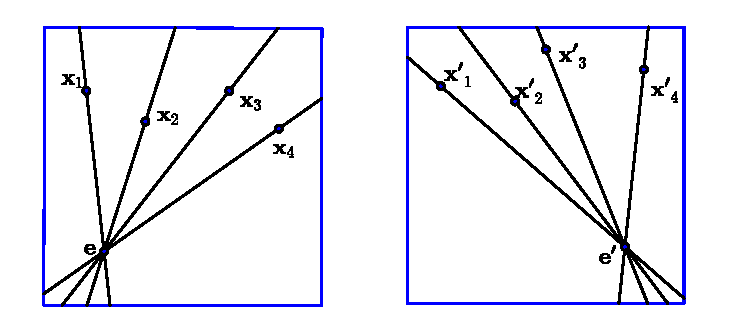
\includegraphics[width=\hsize]{retas-epipolares}
\legend{Feixe de retas passando pelo epipolo em cada imagem, relacionadas duas a duas por uma homografia.}
\source{O autor.}
\label{retas-epipolares}
\end{figure}

\section{O teorema 1: homografia da reta epipolar}\label{sec.homografia-reta-epipolar} 
Uma das primeiras afirmações do artigo é que as retas epipolares numa  imagem estão homograficamente relacionadas com as retas epipolares na segunda imagem. Dados $n$ correspondências de pontos em duas imagens, o teorema trata da \textit{restrição epipolar}, Faugeras (1993). Ou seja, temos uma homografia 1D que relaciona o feixe de retas através ${\bf e}$ com o feixe de retas através ${\bf e'}$ chamada \textit{homografia da reta epipolar}. Podemos visualizar essa situação na Figura \ref{retas-epipolares}.

\begin{teorema}
As $n$ retas passando pelos pontos $\e$ e $\x_i$ na primeira imagem estão homograficamente relacionadas com as $n$ retas passando por $\e'$ e $\x'_i$ na segunda imagem.
\end{teorema}

\begin{proof}
O feixe de retas epipolares em cada imagem estão perspectivamente relacionados através do centro de projeção $Q$ na reta base, conforme a Figura \ref{fig.homo-reta-epipo}.
\begin{figure}[!htb]{\textwidth}
\caption{Perspectiva entre feixes de retas epipolares.}
\includegraphics[width=\hsize]{reta-epipo-2}
\legend{Retas epipolares relacionadas por uma homografia e com perspectiva centrada em {\bf Q}.}
\source{Adaptado, Hartley e Zisserman (2004).}
\label{fig.homo-reta-epipo}
\end{figure}
Suponha que $\lightrgb$ e $\lightrgb'$ sejam duas retas epipolares correspondentes, e ${\bf m}$ é uma reta qualquer que não passa pelo epipolo $\e$. O produto vetorial 
\begin{equation}
{\bf m}\times\lightrgb=\x\qquad\text{ou}\qquad\,[{\bf m}]_\times\,\lightrgb=\x,
\end{equation}
nos fornece o ponto $\x$ de interseção entre essas retas. Pela subseção \ref{sec.matriz-F} temos que
\begin{equation*}
\lightrgb'=F\,\x,
\end{equation*} 
assim, $\lightrgb$ está relacionada a $\lightrgb'$ através da equação 
\begin{equation*}
\lightrgb'=F\,[{\bf m}]_\times\,\lightrgb.
\end{equation*}
Uma boa escolha para ${\bf m}$ é a reta $\e$, já que
\begin{equation*}
{\bf m}^\top\e=\e^\top\e\neq0,
\end{equation*}
então $\e$ é uma reta que não passa pelo epipolo $\e$ como desejado. Assim, a homografia da reta epipolar pode ser escrita como 
\begin{equation*}
\lightrgb'=F\,[\e]_\times\,\lightrgb.
\end{equation*}
O argumento é análogo para o mapeamento da segunda imagem para a primeira,
\begin{equation*}
\lightrgb=F^\top [\e']_\times\,\lightrgb'.
\end{equation*}
\end{proof}
\subsection{Nova abordagem para a homografia da reta epipolar} 


Outra forma de pensar sobre essa homografia é realizando uma translação de forma que os epipolos estejam na origem do plano de cada imagem, e com as retas epipolares passando pelo epipolo, cada reta pode ser parametrizada através do ângulo que ela forma com o eixo das abscissas, denominados $\alpha_1$ e $\alpha_2$ na primeira e segunda imagens respectivamente.
A homografia da reta epipolar pode ser representada pela equação de uma hipérbole alinhada aos eixos perpendiculares, conforme descrito por Fabbri e Kimia (2010b),
\begin{equation}\label{eq.hiperbole}
a\,x\,y+b\,x+c\,y+d=0 \qquad \text{ou} \qquad y=\frac{-b\,x-d}{a\,x+c},
\end{equation} 
onde $x=tan\,\alpha_1$ e $y=tan\,\alpha_2$. 

Vemos na Figura \ref{fig.reta-epipolar} que cada reta epipolar fica definida por um ponto no eixo da tangente, $(1,tan\,\alpha_1)$ na primeira imagem e $(1,tan\,\alpha_2)$ na segunda, onde consideramos o círculo trigonométrico de raio $1$. Usando esses pontos, a equação da hipérbole pode ser escrita na forma
\begin{equation}\label{eq.homo-reta-epi}
(1\,,\,tan\,\alpha_1)
\overbrace{
\begin{bmatrix}
d&c\\
b&a
\end{bmatrix}
}^{H}
\begin{pmatrix}
1\\
tan\,\alpha_2
\end{pmatrix}
=0,
\end{equation}
sendo 
$\begin{bmatrix}d&c\\b&a\end{bmatrix}$ a homografia procurada.

O problema é que a Equação \ref{eq.homo-reta-epi} não está definida para retas epipolares verticais, pois utilizamos a tangente, e uma saída é parametrizar cada reta através da própria definição de tangente, pois assim temos uma representação isotrópica para as retas:
\begin{equation}\label{eq.tan.alpha1-2}
x=tan\,\alpha_1=\frac{sen\,\alpha_1 }{cos\,\alpha_1} \qquad \text{e} \qquad y=tan\,\alpha_2=\frac{sen\,\alpha_2}{cos\,\alpha_2}.
\end{equation} 
Desta forma, substituindo \ref{eq.tan.alpha1-2} em \ref{eq.hiperbole} e multiplicando por $cos\,\alpha_1\,cos\,\alpha_2$ temos
\begin{equation*}
a\,sen\,\alpha_1\,sen\,\alpha_2+b\,sen\,\alpha_1\,cos\,\alpha_2+c\,cos\,\alpha_1\,sen\,\alpha_2+d\,cos\,\alpha_1\,cos\,\alpha_2=0.
\end{equation*}
\begin{figure}[!htb]{10cm}
\caption{Reta epipolar.}
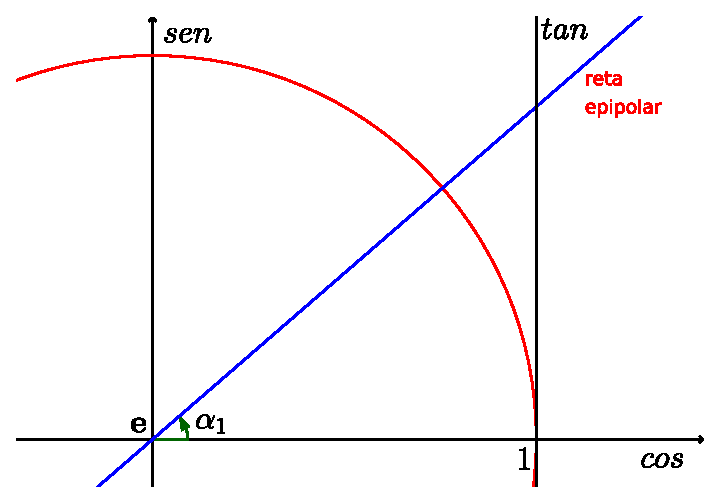
\includegraphics[width=\hsize]{reta-epipolar-alpha1}
\legend{Plano da imagem centrado em ${\bf e}$ com a reta epipolar parametrizada por $\alpha_1$.}
\source{O autor.}
\label{fig.reta-epipolar}
\end{figure}
Com essa conversão, deixamos de parametrizar as retas epipolares pelo eixo das tangentes e passamos a parametrizar pelo círculo trigonométrico. Aqui temos um argumento para contagem dos graus de liberdade para fixarmos a relação entre retas epipolares, pois devemos determinar os dois epipolos (duas variáveis cada totalizando quatro graus de liberdade), e mais a matriz que representa a homografia (quatro variáveis mas apenas três graus de liberdade utilizando uma variável para fixar a escala). Portanto, precisamos de no mínimo sete restrições para determinarmos a relação entre duas imagens na geometria epipolar. 

Na nossa abordagem, consideramos o círculo trigonométrico com raio $1$ mas, segundo Fabbri e Kimia (2010b), podemos estipular raios arbitrários $r_1$ e $r_2$ em cada uma das imagens que ajuda a garantir estabilidade numérica para a determinação dos coeficientes. Assim, obtemos a equação:
\begin{equation*}
a\,r_1\,sen\,\alpha_1\,r_2\,sen\,\alpha_2+b\,r_1\,sen\,\alpha_1\,r_2\,cos\,\alpha_2+c\,r_1\,cos\,\alpha_1\,r_2\,sen\,\alpha_2+d\,r_1\,cos\,\alpha_1\,r_2\,cos\,\alpha_2=0.
\end{equation*}
Em resumo, as vantagens dessa última representação é ser isotrópica e ter boa estabilidade numérica para escolhas convenientes de $r_1$ e $r_2$, e novamente  na representação matricial:
\begin{equation*}
(r_1\,cos\,\alpha_1\,,\,r_1\,sen\,\alpha_1)
\begin{bmatrix}
d&c\\
b&a
\end{bmatrix}
\begin{pmatrix}
r_2\,cos\,\alpha_2\\
r_2\,sen\,\alpha_2
\end{pmatrix}
=0
\end{equation*}
\section{Dedução da IAC}

Uma ferramenta algébrica bastante utilizada nessa abordagem de Nist\'er e Schaffalitzky (2006) é a imagem da cônica absoluta (IAC em inglês) denotada por ${\bf \omega}$. Como a abordagem assume que as câmeras são calibradas, vamos mostrar que é possível obter a IAC em função da matriz de calibração da câmera, $K$.

\subsection{Calibração e a imagem da cônica absoluta}\label{sec.omega-calibracao}

 Inicialmente, vamos determinar a homografia que faz o mapeamento do plano no infinito $\bpi_\infty$ para o plano da imagem na câmera. Se $\X_\infty\in\bpi_\infty$ então pode ser escrito na forma
\begin{equation*}
\X_\infty=({\bf d}^\top,0)^\top
\end{equation*} 
e é projetado por uma câmera geral $P=K\,[R|{\bf t}]$ como
\begin{equation*}
\begin{array}{rcl}
\x&=&P\,\X_\infty\\
&=&K\,[R|{\bf t}]\,({\bf d}^\top,0)^\top\\
&=&K\,R\,{\bf d}.
\end{array}
\end{equation*}
Portanto temos a relação
\begin{equation*}
\x=H\,{\bf d}
\end{equation*}
onde $H=K\,R$. Como a cônica absoluta $\Omega_\infty$ está contida no plano no infinito (contém pontos no infinito), ela pode ser projetada sob a homografia $H$ para computarmos sua imagem.
Sob uma homografia de ponto $\x\rightarrow H\,\x$, uma cônica se transforama de acordo com $C\rightarrow H^{-\top} C\,H^{-1}$, conforme a subseção \ref{sec.trans-proj-H}. De acordo com a subseção \ref{sec.con-absoluta}, $C=\Omega_\infty =I$, daí temos
\begin{equation*}
\begin{array}{rcl}
{\bf \omega}&=&H^{-\top}\Omega_\infty\,H^{-1}\\
&=&(K\,R)^{-\top}\,I\,(K\,R)^{-1}\\
&=&K^{-\top}R^{-\top}R^{-1}K^{-1}\\
&=&K^{-\top}K^{-1}
\end{array}
\end{equation*}
pois $R$ é uma matriz de rotação e portanto satisfaz $R^{-\top}R^{-1}=I$. Assim, de posse de uma câmera calibrada é simples obter a IAC.

Analogamente ao que é feito na subseção \ref{sec.conica-dual}, podemos definir a imagem dual da cônica absoluta (sigla DIAC em inglês), denotada por $\omega^*$, a partir de $\omega$ como
\begin{equation*}
\omega^*=\omega^{-1}=K\,K^\top.
\end{equation*}
Esta é uma cônica definida por retas e é a imagem da quádrica dual absoluta ${\tt Q^*_\infty}$, definida na subseção \ref{sec.quadrica-dual-abs}. A imagem é dada por
\begin{equation*}
\omega^*=P\,{\tt Q^*_\infty}P^\top,
\end{equation*}
conforme a subseção \ref{sec.proj-quadricas}. Nota-se que tais objetos geométricos são apenas artifícios para se trabalhar com a informada matriz $K$.

\section{O teorema 2: restrição Kruppa}\label{sec.teorema-2}

A correspondência entre retas tangentes às duas cônicas ${\bf \omega}$ e ${\bf \omega'}$ é conhecida como a restrição \textit{Kruppa}. Na Figura \ref{epipolar-kruppa} podemos observar as restrições epipolar e Kruppa simultaneamente.
\begin{figure}[!htb]{\textwidth}
\caption{Restriç\~oes Kruppa e epipolar.}
\includegraphics[width=\hsize]{restricao-epipolar-kruppa}
\legend{Retas epipolares tangentes às cônicas ${\bf \omega}$ e ${\bf \omega'}$.}
\source{O autor.}
\label{epipolar-kruppa}
\end{figure}
A restrição Kruppa foi originalmente introduzida por Faugeras e Maybank (1992) e está relacionada com uma cônica contida num plano no espaco 3D e suas imagens nas duas câmeras, e é válida para cônicas gerais, mas aqui no nosso caso vamos tratar especificamente da cônica absoluta $\Omega_\infty$ contida no plano infinito $\bpi_\infty$ no espaço, e as imagens da cônica absoluta (IAC) ${\bf \omega}$ e ${\bf \omega'}$.

\begin{teorema}
As duas tangentes à IAC $\omega$ passando pelo epipolo $\e$ estão relacionadas por uma homografia da reta epipolar às duas tangentes à IAC $\omega'$ passando pelo epipolo $\e'$.
\end{teorema}

\begin{proof}
 Sendo ${\bf \omega}^*$ e ${{\bf \omega}^*}'$ as respectivas cônicas duais (DIAC), considere um plano passando pelo centro das duas câmeras e tangenciando essa cônica $\Omega_\infty$ no espaço. Por construção, esse plano vai projetar uma reta epipolar em cada imagem onde cada reta será tangente às imagens ${\bf \omega}$ e ${\bf \omega'}$ da cônica $\Omega_\infty$, observado na Figura \ref{geometria-kruppa}. E suponha ainda que $\lightrgb_1$ e $\lightrgb_2$ sejam as retas tangentes à cônica ${\bf \omega}$ na primeira imagem conforme a Figura \ref{epipolar-kruppa}. Com essas duas retas tangentes podemos construir uma cônica degenerada $D$ (posto $2$) na forma  
\begin{equation}\label{eq.def.con.deg}
D=[\e]_\times\,{\bf \omega}^*\,[\e]_\times. 
\end{equation}
Para mostrar que $D$ é uma cônica (ponto) temos que verificar que é válida a relação $\y_1^\top D\,\y_1=0$, onde $\y_1\in\lightrgb_1$.
\begin{equation*}
\begin{array}{rcll}
\y_1^\top\,D\,\y_1&=&\y_1^\top [\e]_\times\,{\bf \omega}^*\,[\e]_\times\,\y_1&\\
&=&([\e]^\top_\times\,\y_1)^\top {\bf \omega}^*\,[\e]_\times\,\y_1&\\
&=&\lightrgb_1^\top {\bf \omega}^*\,\lightrgb_1& \qquad\text{pois}\qquad\lightrgb_1=\e\times\y_1\\
&=&0&
\end{array}
\end{equation*}
onde a última passagem segue do fato de ${\bf \omega}^*$ ser dual. Observe que usamos $[\e]^\top_\times\,\y_1=[\e]_\times\,\y_1$ quando na verdade $[\e]^\top_\times=-[\e]_\times$, mas aqui a diferença de escala é irrelevante.
\begin{figure}[!htb]{\textwidth}
\caption{Homografia planar e a restric\~ao Kruppa.}
\includegraphics[width=\hsize]{geometria-kruppa}
\legend{Um plano epipolar tangenciando uma cônica no espaco 3D projeta retas epipolares que tangenciam as cônicas nos planos das imagens.}
\source{Hartley e Zisserman (2004).}
\label{geometria-kruppa}
\end{figure}
Observamos que o desenvolvimento anterior é análogo para $\lightrgb_2$.

Na segunda imagem, analogamente à primeira, $D'=[\e']_\times\,{{\bf \omega}^*}'\,[\e']_\times$ e se transforma de acordo com a regra $D'=H_\infty^{-\top}D\,H_\infty^{-1}$ na subseção \ref{sec.trans-proj-H}. O símbolo $\infty$ se deve ao fato de que a homografia foi deduzida de maneria similar àquela da subseção  \ref{sec.homografia}, apenas com a diferença de ter sido com base no plano no infinito. Assim:
\begin{equation}\label{eq.kruppa}
\begin{array}{rcll}
[\e']_\times\,{{\bf \omega}^*}'\,[\e']_\times&=&D'&\\
&=&H_\infty^{-\top}D\,H_\infty^{-1}&\\
&=&H_\infty^{-\top}[\e]_\times\,{\bf \omega}^*\,[\e]_\times\,H_\infty^{-1}&\qquad\text{pois}\qquad D=[\e]_\times\,{\bf \omega}^*\,[\e]_\times\\
%&=&F\,\omega^* F^\top,&
\end{array}
\end{equation}
%onde $F=H_\infty^{-\top}\,[\e]_\times$ conforme a %subseção \ref{sec.matriz-F}. 
Como $\omega$ é uma cônica envelope, as retas que são tangentes à $\omega$ satisfazem a equação de $\omega^*$, e temos que essas tangentes estão projetivamente relacionadas, em conjunto, pela Equação \ref{eq.kruppa}. Como as tangentes passam pelos epipolos, são retas epipolares e o teorema segue.
\end{proof}
Observa-se que, como conjunto, as tangentes não vêm em qualquer ordem particular, pois a relação não explicita uma mapeamento individual entre as retas, há apenas a relação entre produtos simétricos. Mas veremos na Subseção \ref{sec.teorema-5} que esse fato não causará problemas.
\section{Mudança de coordenadas projetivas}

De acordo com Semple e Kneebone (1952), podemos escolher as coordenadas projetivas de forma que os quatro pontos tenham as mesmas coordenadas em cada imagem. Ou seja, podemos assumir que ${\bf x}_i = {\bf x'}_i$ pensando nos dois planos de imagem como registrados no mesmo sistema de coordenadas. Vejamos como isso pode ser feito.

\subsection{Corregistro de pontos pertencentes a diferentes planos de imagem}\label{sec.corregistro-pontos}
Suponha a existência de pontos correspondêntes em dois planos de imagem relacionados por uma transformação projetiva $\x'=H\,\x$, onde $\x\in {\mathbb{P}^2}$ e $\x'\in {\mathbb{P'}^2}$. Nosso objetivo é fazer o corregistro de pontos da segunda imagem no sistema de coordenadas da primeira imagem, mas também poderíamos fazer o corregistro dos pontos das duas imagens para um terceiro plano projetivo qualquer. Fazendo as seguintes mudanças de coordenadas projetivas
\begin{equation}\label{eq.igualando-coordenadas}
\begin{array}{rcl}
\overline{\x}\,&=&I\,\x\\
\overline{\x}'&=&H^{-1}\x',
\end{array}
\end{equation}
temos que $\x=\overline{\x}$ e $\x'=H\,\overline{\x}'$. Substituindo essas duas últimas igualdades em $\x'=H\,\x$ temos
\begin{equation*}
\begin{array}{rcll}
\x'&=&H\,\x&\Rightarrow\\
H\,\overline{\x}'&=&H\,\overline{\x}&\Rightarrow\\
\overline{\x}'&=&H^{-1}H\,\overline{\x}&\Rightarrow\\
\overline{\x}'&=&\overline{\x}.&
\end{array}
\end{equation*}
Cabe ressaltar que as mudanças de coordenadas em \ref{eq.igualando-coordenadas} não altera nosso desenvolvimento, já que aqui nos interessa propriedades que são invariantes sob transformações projetivas, como tangências, interseções e raz\~ao cruzada. Portanto, onde foi utilizada a matriz identidade poderia ter sido usada qualquer outra homografia no caso de transferência dos pontos para um terceiro plano qualquer. A homografia $H$ é determinada a partir dos quatro pontos correspondentes supostos inicialmente pelo artigo.
\section{O teorema 3: pontos e epipolos co-cônicos}\label{sec.teorema-3}

Aplicando as mudanças de coordenadas descritas na Subsec\~ao \ref{sec.corregistro-pontos} nos quatro pontos e nos epipolos, temos que $\x=\x'$ e todos os seis pontos em questão estarão expressos no mesmo sistema de coordenadas, no mesmo plano de imagem. Observe a Figura \ref{pontos-conconicos}.

\begin{teorema}
Os epipolos $\e$, $\e'$ e os quatro pontos $\x_i$ na imagem devem pertencer a uma cônica $B$. Reciprocamente, dois epipolos que são co-cônicos com os quatro pontos na imagem devem satisfazer à restricão epipolar.
\end{teorema}

\begin{proof}
Pela subseção \ref{sec.definicao-conica}, uma cônica fica determinada por cinco pontos, como temos quatro pontos na imagem vamos deixar a cônica $B$ na dependência de $\e$ (o quinto ponto necessário). Analogamente, o epipolo $\e'$ também define uma cônica com os quatro pontos na imagem, digamos $B'$. Pela subsec\~ao \ref{sec.homografia-reta-epipolar}, existe a homografia da reta epipolar que relaciona as quatro retas do feixe passando por $\e$ com as quatro retas do feixe passando por $\e'$. Fazendo o corregistro dos pontos e pelo teorema de Steiner, em Semple e Kneebone (1952), se dois feixes de retas passando por $\e$ e $\e'$ estão homograficamente relacionados, o ponto de interseção entre retas correspondentes desses feixes descreve uma cônica que passa por $\e$ e $\e'$. Portanto $B=B'$ e todos os seis pontos em questão são co-cônicos.


Reciprocamente, pelo teorema de Chasles em Semple e Kneebone (1952), se quatro pontos $\x_i \in B$ formam um feixe de retas concorrentes em um quinto ponto $\e\in B$, a razão cruzada entre as quatro retas não depende da posição de $\e$. Assim, a razão cruzada  do feixe concorrente em $\e$ é igual a do feixe concorrente em $\e'$. Pela subseção \ref{sec.geometria-1D}, a razão cruzada num feixe de retas é igual a razão cruzada entre os quatro pontos de interseção de uma reta qualquer com o feixe. Pelo corolário ainda na subseção \ref{sec.geometria-1D}, dois conjuntos de quatro pontos colineares têm a mesma razão cruzada se, e somente se, correspondem sob uma homografia.  Pela dualidade da representação entre pontos e retas, temos a homografia entre retas epipolares.  
\end{proof}

Esta cônica $B=B(\e)$ será bastante importante durante a abordagem pois, se os dois epipolos são co-cônicos com os quatro pontos na imagem, Figura \ref{pontos-conconicos}, existe uma \textit{única} homografia de reta epipolar que faz a relação das retas através ${\bf e}$ com as retas através ${\bf e'}$.
\begin{figure}[!htb]{.7\textwidth}
\caption{Pontos co-c\^onicos.}
\includegraphics[width=\hsize]{pontos-conconicos}
\legend{Epipolos co-cônicos com os quatro pontos na imagem produzem homografia única.}
\source{O autor.}
\label{pontos-conconicos}
\end{figure}
\section{O teorema 4: interseção das tangentes}\label{sec.demonstracao-teo-4}

Nota-se que podemos parametrizar o feixe de retas passando por ${\bf e'}$ (ou ${\bf e}$) por pontos pertencentes à cônica $B$, pois retas correspondentes nos dois feixes interceptam $B$ no mesmo ponto. 

\begin{teorema}
As restrições de calibração são equivalentes à condição de que duas retas tangentes a\, $\omega$ que passam por $\e$ intersectam a cônica $B$ nos mesmos dois pontos adicionais que as duas retas tangentes a $\omega'$ passando por $\e'$.
\end{teorema}

\begin{proof}
Na subseção \ref{sec.teorema-2}, vimos que as duas retas tangentes à conica $\omega$ estão projetivamente relacionadas com as duas tangentes à cônica $\omega'$. Pelo teorema de Steiner, o ponto de interseção entre duas retas correspondentes, em dois feixes homograficamente relacionados, descrevem uma cônica. Assim, as retas tangentes à cônica $\omega$ se interceptam às retas tangentes à cônica $\omega'$ em dois pontos adicionais sobre a cônica $B$. 
\end{proof}

Isto é, as projeções de ${\bf \omega}$ e ${\bf \omega'}$ em $B$, através dos respectivos epipolos, devem coincidir. Essa construção geométrica pode ser visualizada na Figura \ref{omega-B} e será a fundação para o resto da abordagem. 
\begin{figure}[!htb]{.7\textwidth}
\caption{Interseç\~ao entre $B$ e as tangentes.}
\includegraphics[width=\hsize]{projecao-omega-B}
\legend{Os pontos de interseção das tangentes com a cônica $B$ coincidem, ocasionando a coincidência das projeções das cônicas ${\bf \omega}$ e ${\bf \omega'}$ na cônica $B$.}
\source{O autor.}
\label{omega-B}
\end{figure}
\section{O teorema 5: projeção de $\omega$ em $B$}\label{sec.teorema-5}

 A demonstração do próximo teorema é dada por Nist\'er e Schaffalitsky (2006), mas vamos incluir alguns detalhes e posteriormente dar uma demonstração extendida. Acompanhando pela Figura \ref{omega-B}, podemos pensar na representação da projeção de  ${\bf \omega}$ e ${\bf \omega'}$ em $B$ como a reta que liga os dois pontos de interseção das tangentes com $B$, pois tal fato vai resolver o problema de que as tangentes não têm ordenação específica. Essa reta que liga os dois pontos de interseção, de acordo com a projeção de ${\bf \omega}$ através do epipolo ${\bf e}$ é representada por $({\bf \omega}\diamond B)\,{\bf e}$.

A Equação \ref{eq.conica-diamond} é uma fórmula projetivamente invariante de uma cônica. Para ver isso, basta tomar a configuração para as cônicas $B$ e $\omega^*$ (mais a frente veremos o porquê dessas configurações)
\begin{equation*}
B=
\begin{bmatrix}
0&0&1\\
0&-2&0\\
1&0&0
\end{bmatrix}
\qquad\text{e}\qquad
\omega^*=
\begin{bmatrix}
c_{11}&c_{12}&c_{13}\\
c_{12}&c_{22}&c_{23}\\
c_{13}&c_{23}&c_{33}
\end{bmatrix},
\end{equation*} 
e efetuar as multiplicações constantes na Equação \ref{eq.conica-diamond}. Lembrando que o traço de uma matriz é definido pela soma dos elementos da diagonal principal, o resultado das multiplicações é uma matriz simétrica, que pela subseção \ref{sec.definicao-conica}, representa uma cônica. Pela subseção \ref{sec.trans-proj-H}, uma homografia leva uma cônica em outra cônica, a qual mantém as características invariantes sob transformação projetiva.
\subsection{Representação canônica de uma cônica}\label{sec.forma-canonica-B}

Como vimos na subseção \ref{sec.espaco-P2}, o plano projetivo $\mathbb{P}^2$ tem seus pontos representados por vetores homogêneos com três componentes. Da álgebra linear sabemos que o espaço $\mathbb{R}^3$ também tem seus pontos representados por vetores com três componentes. Portanto, existe uma analogia entre as representações mesmo que no plano projetivo a relação entre vetores e pontos não seja biunívoca como em $\mathbb{R}^3$. Da mesma forma que podemos escolher a base canônica para representar vetores em $\mathbb{R}^3$, fazendo a devida transformação projetiva do sistema de coordenadas, podemos escolher uma base para representação do plano projetivo com a inclusão de um \textit{vetor unitário} ${\bf u}=(1,1,1)^\top$. Assim, cada ponto em $\mathbb{P}^2$ pode ser representado em termos da base \{$\x_1=(1,0,0)^\top,\x_2=(0,1,0)^\top,\x_3=(0,0,1)^\top,{\bf u}=(1,1,1)^\top$\} onde os três primeiros vetores são chamados {\it pontos de referência}. Para detalhes ver teorema 1 no apêndice  de Semple e Kneebone (1952).

Os pontos de referência, que são linearmente independentes, formam os vértices de um triângulo chamado \textit{triângulo de referência}, com o ponto unitário no interior do triângulo. Esse triângulo vai servir como uma base para a representação do plano projetivo, conforme a Figura \ref{fig.triangulo-referencia}. Por exemplo, representando um ponto qualquer por $\x=(x,y,z)^\top$ e uma reta qualquer por $\lightrgb=(a,b,c)^\top$ a reta determinada pelos pontos $\x_1$ e ${\bf u}$ tem equação $z-y=0$.
\begin{figure}[!htb]{.7\textwidth}
\caption{Tri\^angulo de refer\^encia.}
\includegraphics[width=\hsize]{triangulo-referencia}
\legend{Triângulo de referência com vértices determinados por três vetores que, juntamente com o vetor unitário, servem de base para representação do plano projetivo.}
\source{O autor.}
\label{fig.triangulo-referencia}
\end{figure}
De fato, se $\x_1\in\lightrgb$ e ${\bf u}\in\lightrgb$ então
\begin{equation}\label{eq.exemplo-tri-referencia}
\lightrgb^\top{\bf u}=0\Rightarrow a+b+c=0\qquad\text{e}\qquad\lightrgb^\top\x_1=0\Rightarrow a=0.\qquad\text{Assim,}\quad b=-c.
\end{equation}
Dado um ponto qualquer $\x\in\lightrgb$ a equação da reta fica
\begin{equation*}
\lightrgb^\top\x=0\Rightarrow a\,x+b\,y+c\,z=0,
\end{equation*}
e usando as Relações \ref{eq.exemplo-tri-referencia} temos que
\begin{equation*}
-c\,y+c\,z=0\Rightarrow z-y=0,
\end{equation*}
já que $c\neq 0$ pois do contrário $\lightrgb=(0,0,0)^\top$ e não representaria reta alguma, conforme a subseção \ref{sec.reta}. 

Existem algumas formas padronizadas pelas quais a representação da cônica $B$ pode ser simplificada através da escolha conveniente de uma estrutura de referência. Uma dessas escolhas é tomar o triângulo de referência como tendo dois de seus lados tangentes à cônica, e o terceiro lado como reta polar em relação ao seu vértice oposto, e escolher um ponto  da cônica como ponto unitário. Ver Figura \ref{fig.conica-tri-referencia}.
\begin{figure}[!htb]{.7\textwidth}
\caption{Relação polo-polar.}
\includegraphics[width=\hsize]{conica-tri-referencia}
\legend{A cônica $B$ numa relação polo-polar com um triângulo de referência que representa o plano projetivo $\mathbb{P}^2$.}
\source{O autor.}
\label{fig.conica-tri-referencia}
\end{figure}
Como vimos na subseção \ref{sec.definicao-conica}, a cônica $B$ pode ser representada na forma matricial com coordenadas homogêneas como
\begin{equation*}
\begin{pmatrix}
x&y&z
\end{pmatrix}
\begin{bmatrix}
a&b/2&c/2\\
b/2&d&e/2\\
c/2&e/2&f
\end{bmatrix}
\begin{pmatrix}
x\\
y\\
z
\end{pmatrix}
=0
\end{equation*}
ou através da equação
\begin{equation*}
a\,x^2+b\,x\,y+d\,y^2+c\,x\,z+e\,y\,z+f\,z^2=0.
\end{equation*}
Supondo que a cônica passe pelos pontos $\x_1=(1,0,0)^\top$ e $\x_3=(0,0,1)^\top$ temos que
\begin{equation*}
\x_1\in B\Rightarrow a=0\quad\text{e}\quad\x_3\in B\Rightarrow f=0,
\end{equation*}
daí a equação da cônica será 
\begin{equation}\label{eq.reducao-parcial-conica}
d\,y^2+b\,x\,y+c\,x\,z+e\,y\,z=0.
\end{equation}
Consirede a reta $\lightrgb=(l_1,l_2,l_3)^\top$ que passa pelos pontos $\x_1$ e $\x_3$,
\begin{equation*}
\lightrgb^\top\x_1=
\begin{pmatrix}
l_1&l_2&l_3
\end{pmatrix}
\begin{pmatrix}
1\\
0\\
0
\end{pmatrix}
=0
\Rightarrow l_1=0,
\end{equation*} 
\begin{equation*}
\lightrgb^\top\x_3=
\begin{pmatrix}
l_1&l_2&l_3
\end{pmatrix}
\begin{pmatrix}
0\\
0\\
1
\end{pmatrix}
=0
\Rightarrow l_3=0,
\end{equation*} 
e portanto $\lightrgb=(0,l_2,0)^\top$.
Observando que $\lightrgb$ está numa relação polo-polar com o ponto $\x_2$, pela subseção \ref{sec.polo-polar} temos que $B\,\x_2=\lightrgb$, daí
\begin{equation*}
\begin{bmatrix}
a&b/2&c/2\\
b/2&d&e/2\\
c/2&e/2&f
\end{bmatrix}
\begin{pmatrix}
0\\
1\\
0
\end{pmatrix}
=
\begin{pmatrix}
b/2\\
d\\
e/2
\end{pmatrix}
=
\begin{pmatrix}
0\\
l_2\\
0
\end{pmatrix},
\end{equation*}
e teremos $b=e=0$ e $d=l_2$.
E como $l_2 \neq 0$ a Equação \ref{eq.reducao-parcial-conica} toma a forma
\begin{equation}\label{eq.reducao-parcial2-conica}
l_2\,y^2+c\,x\,z=0,\quad\text{ou}\quad y^2=k\,x\,z\quad\text{com}\quad k=-\frac{c}{l_2}.
\end{equation}
A cônica $B$ passa também pelo ponto unitário ${\bf u}=(1,1,1)^\top$, assim substituindo na Equação \ref{eq.reducao-parcial2-conica} temos que $k=1$, e a equação da cônica se reduz finalmente a 
\begin{equation}\label{eq.reducao-total-conica}
y^2=x\,z,
\end{equation}
que é a equação conônica da cônica em $\mathbb{P}^2$. Na forma matricial a cônica é representada por 
\begin{equation*}
B=
\begin{bmatrix}
0&0&1\\
0&-2&0\\
1&0&0
\end{bmatrix}.
\end{equation*}
\subsection{Representação canônica paramétrica}\label{sec.repre-canonica-parametrica}
A Equação \ref{eq.reducao-total-conica} pode ser escrita na forma 

\begin{equation*}
\left(\frac{y}{z}\right)^2=\frac{x}{z},
\end{equation*}
e fazendo a substituição $\displaystyle{\frac{y}{z}=\theta}$ temos que $\displaystyle{\frac{x}{z}=\theta^2}$ e $x:y:z=\theta^2:\theta:1$.
Assim, todo ponto pertencente à cônica $B$ terá a forma $(\theta^2,\theta,1)^\top$, que é realmente uma parametrização da curva, no sentido de que existe uma relação biunívoca entre cada ponto da curva e o valor do parâmetro $\theta$. No caso do artigo de Nist\'er e Schaffalitzky (2006) esta formalização é bastante útil pois, como a cônica $B$ está em função do quinto ponto, o epipolo $\e$, temos que esse ponto, e consequentemente a cônica, pode ser definida apenas pelo parâmetro $\theta$. Podemos observar que é válida a relação

\begin{equation*}
\begin{pmatrix}
1&\theta&\theta^2
\end{pmatrix}
\begin{bmatrix}
0&0&1\\
0&-2&0\\
1&0&0
\end{bmatrix}
\begin{pmatrix}
1\\
\theta\\
\theta^2
\end{pmatrix}
=0.
\end{equation*}


\subsection{Demonstração do teorema}

Após a apresentação dos conceitos necessários, vamos estabelecer o teorema e demonstrá-lo em detalhes.

\begin{teorema}
A projeção da IAC $\omega$ na cônica $B$, usando o epipolo $\e$ como centro de projeção, é dada pelos pontos de interseção entre a reta $(\omega\diamond B)\,\e$ e $B$, onde a cônica $(\omega\diamond B)$ é definida como

\begin{equation}\label{eq.conica-diamond}
(\omega \diamond B)\equiv 2\,B\,\omega^*B - tr(\omega^*\,B)\,B.
\end{equation}
\end{teorema}

\begin{proof}

Pela subseção \ref{sec.demonstracao-teo-4}, a reta epipolar $\lightrgb$ tangente à IAC intercepta a cônica $B$ em um ponto ${\bf q}$, conforme a Figura \ref{omega-B}. Como ${\bf q}\in B$ e $B$ tem a forma definida na subseção \ref{sec.forma-canonica-B}, temos que ${\bf q}$ pode ser parametrizado por ${\bf q}=(1,\lambda,\lambda^2)^\top$, conforme a subseção \ref{sec.repre-canonica-parametrica}. Desta forma, precisamos mostrar que ${\bf q}\in (\omega\diamond B)\,\e$, ou seja, $[(\omega\diamond B)\,\e]^\top {\bf q}=0$ onde $\e=(1,\theta,\theta^2)^\top$. A reta $\lightrgb$ pode ser definida pelos pontos $\e$ e ${\bf q}$ como $\lightrgb=\e\times {\bf q}$ e, fazendo as substituições, vem

\begin{equation*}
\begin{array}{rcl}
\lightrgb&=&(1,\theta ,\theta^2)\times (1,\lambda,\lambda^2)\\
&=&(\lambda -\theta)(\theta\lambda,-(\theta+\lambda),1)\\
&=&(\theta\lambda,-(\theta+\lambda),1)
\end{array}
\end{equation*}
ignorando o fator de escala $(\lambda-\theta)$.
Como $\lightrgb$ é tangente à cônica $\omega$, temos que a reta satisfaz a relação definida na Subseção \ref{sec.conica-dual}, $\lightrgb^\top\omega^*\lightrgb=0$. Parametrizando $\omega^*$ por $[c_{ij}]$ temos que a relação $\lightrgb^\top\omega^*\lightrgb=0$ se torna

\begin{equation*}
\begin{pmatrix}
\theta\lambda&-(\theta+\lambda)&1
\end{pmatrix}
\begin{bmatrix}
c_{11}&c_{12}&c_{13}\\
c_{12}&c_{22}&c_{23}\\
c_{13}&c_{23}&c_{33}
\end{bmatrix}
\begin{pmatrix}
\theta\lambda\\
-(\theta+\lambda)\\
1
\end{pmatrix}
=0,
\end{equation*}  
que é equivalente à equação
\begin{equation}\label{eq.expandida-omega-dual}
\theta^2\lambda^2 c_{11}+(-2\,\theta^2\,\lambda-2\,\theta\lambda^2)\,c_{12}+2\,\theta\lambda\,c_{13}+(\theta+\lambda)^2\,c_{22}+(-2\,\theta-2\,\lambda)\,c_{23}+c_{33}=0.
\end{equation} 
Usando a definição de $(\omega\diamond B)$ em \ref{eq.conica-diamond}, a parametrização de $\omega^*$ por $[c_{ij}]$ e a forma canônica de $B$ (subseção \ref{sec.repre-canonica-parametrica}), temos que

\begin{equation*}
(\omega\diamond B)=
\begin{bmatrix}
2\,c_{33}&-4\,c_{23}&2\,c_{22}\\
-4\,c_{23}&4\,(c_{13}+c_{22})&-4\,c_{12}\\
2\,c_{22}&-4\,c_{12}&2\,c_{11}
\end{bmatrix},
\end{equation*}
e a relação $[(\omega\diamond B)\,\e]^\top {\bf q}=\e^\top (\omega\diamond B)\,{\bf q}=0$ se torna

\begin{equation*}
\begin{pmatrix}
1&\theta&\theta^2
\end{pmatrix}
\begin{bmatrix}
2\,c_{33}&-4\,c_{23}&2\,c_{22}\\
-4\,c_{23}&4\,(c_{13}+c_{22})&-4\,c_{12}\\
2\,c_{22}&-4\,c_{12}&2\,c_{11}
\end{bmatrix}
\begin{pmatrix}
1\\
\lambda\\
\lambda^2
\end{pmatrix}
=0,
\end{equation*}
que é equivalente à equação
\begin{equation}\label{eq.expandida-omega-diamond}
\theta^2\lambda^2 c_{11}+(-2\,\theta^2\,\lambda-2\,\theta\lambda^2)\,c_{12}+2\,\theta\lambda\,c_{13}+(\theta+\lambda)^2\,c_{22}+(-2\,\theta-2\,\lambda)\,c_{23}+c_{33}=0,
\end{equation}
a menos do fator de escala 2. A Equação \ref{eq.expandida-omega-dual} é igual a Equação \ref{eq.expandida-omega-diamond}, e como 
\ref{eq.expandida-omega-dual} é uma relação válida, também é a Equação \ref{eq.expandida-omega-diamond}. O teorema segue.
\end{proof}
O desenvolvimento é análogo para o ponto de interseção das demais tangentes com $B$.
\section{O teorema 6: projeção de $\omega'$ em $B$}\label{sec.teorema-6}

\begin{teorema}
Dado que os epipolos $\e$ e $\e'$ são co-cônicos com quatro pontos na imagem, a restrição Kruppa é equivalente à restricao de que as retas $(\omega\diamond B)\,\e$ e $(\omega'\diamond B)\,\e'$ coincidem.
\end{teorema}

\begin{proof}
Pela Subseção \ref{sec.demonstracao-teo-4}, as retas tangentes à $\omega'$ intersectam $B$ nos mesmos pontos adicionais, onde um deles foi denotado por ${\bf q}$. Como os pontos são co-cônicos podemos usar a forma canônica de $B$ e a parametrização canônica para $\e'$. O desenvolvimento é análogo ao da subseção \ref{sec.teorema-5}.
\end{proof}

\section{O teorema 7: a função que relaciona os epipolos}


Primeiramente nota-se que $(\omega \diamond B) = B\,(\omega \cdot B)$ se definirmos a homografia
\begin{equation}
(\omega \cdot B) \equiv 2\,\omega^*\,B - tr(\omega^*\,B)\,I,
\end{equation}
onde $B$ está sendo ``cancelado" na definição de $(\omega \diamond B)$. Antes de passarmos ao teorema vamos fazer um esclarecimento sobre alguns conceitos. 

\subsection{Feixe de cônicas}\label{sec.feixe-conicas}

Dadas duas cônicas $B_1$ e $B_2$ pertencentes a $\mathbb{P}^2$, cujo a forma quadrática é definida por $\x^\top B_1\x=0$ e $\x^\top B_2\x=0$, chamamos de \textit{feixe de cônicas} a família de cônicas definidas por
\begin{equation}\label{eq.B-combinacao-B1-B2}
B=\lambda\,B_1+\mu\,B_2\quad\text{onde}\quad\x\in\mathbb{P}^2.
\end{equation}
Observe que as cônicas $B_1$ e $B_2$ também pertencem ao feixe, onde basta tomarmos os valores $\lambda=1$ e $\mu=0$ e vice-versa para verificarmos tal fato. Assim, quaisquer duas cônicas pertencentes ao feixe podem ser escolhidas como uma base para a representação do feixe. Resolvendo o sistema de equações
\begin{empheq}[left=\empheqlbrace]{align*}
\x^\top B_1\x&=0\\
\x^\top B_2\x&=0
\end{empheq}
temos vários casos para as soluções mas trataremos aqui somente do caso com quatro soluções distintas, já que Nist\'er e Schaffalitzky (2006) pressupõe que sejam fornecidos quatro pontos em posições gerais no plano da imagem, os quais são utilizados na definição do feixe de cônicas.

Chamamos de {\it pontos base} de um feixe de cônicas, os pontos que são comuns a todas as cônicas do feixe, isto é, eles são os pontos de interseção das duas cônicas $B_1$ e $B_2$ que são a base do feixe. Assim, o feixe de cônicas fica definido pelos quatro pontos de interseção dessas duas cônicas.

Como os quatro pontos $\x_i$ que definem o feixe são todos diferentes, temos que o feixe contém exatamente três cônicas degeneradas que são constituídas por pares de retas. Definindo as retas por dois pontos temos um total de combinações de $C_{4,2}=6$ retas dadas por
\begin{equation*}
\lightrgb_k=\x_i\times\x_j\quad\text{com}\quad k=1,...,6,\,\,i=1,2,3,\,\,j=2,3,4,\quad\text{e}\quad i<j.
\end{equation*}
Pela subseção \ref{sec.conicas-degeneradas}, cada cônica degenerada do feixe pode ser expressa como
\begin{equation}
\begin{array}{rcl}
B_1&=&\lightrgb_1\lightrgb_2^\top+\lightrgb_2\lightrgb_1^\top\\
B_2&=&\lightrgb_3\lightrgb_4^\top+\lightrgb_4\lightrgb_3^\top\\
B_3&=&\lightrgb_5\lightrgb_6^\top+\lightrgb_6\lightrgb_5^\top.
\end{array}
\end{equation}
Observa-se que com seis retas temos um total de combinações de $C_{6,2}=15$ cônicas, no entanto duas retas escolhidas devem passar pelos quatro pontos base, ou seja, duas retas não podem compartilhar um mesmo ponto base. Portanto temos apenas três cônicas degeneradas, as quais são normalmente usadas como base do feixe de cônicas por serem mais facilmente obtidas.
 
\subsection{Estabelecimento e demonstração do teorema}\label{sec.teorema-7}

O esquema para o próximo teorema está representado na Figura \ref{inter-B-C} e o símbolo $\sim$ significa igualdade a menos da escala.
\begin{teorema}
Os epipolos estão ralacionados por 
\begin{equation}\label{eq.equiv-reta-polar-sem-B}
(\omega'\cdot B)\,\e'\sim (\omega\cdot B)\,\e\sim{\bf p}
\end{equation}
o que implica numa função de sétimo grau 
\begin{equation}\label{eq.map-7-grau}
{\bf e} \rightarrow {\bf e'} \sim (\omega' \cdot B)^*\,(\omega \cdot B)\,{\bf e}.
\end{equation}
A restrição Kruppa disponibiliza quatro soluções para o epipolo ${\bf e}$ na cônica $B$, e as soluções são as interseções  de $B$ com a curva 
\begin{equation}\label{eq.definicao-conica-C}
C \equiv (\omega \cdot B)^\top\,(\omega' \cdot B)^{*\,\top}\,B\,(\omega' \cdot B)^*(\omega \cdot B).
\end{equation}
\end{teorema}

\begin{proof}
Pela subseção \ref{sec.teorema-6} $(\omega\diamond B)\,\e\sim(\omega'\diamond B)\,\e'$, e como a cônica $B$ é própria (posto completo) podemos invertê-la e eliminá-la na definição de $(\omega\diamond B)$ e de $(\omega'\diamond B)$ para chegar à Relação \ref{eq.equiv-reta-polar-sem-B}. Assumindo que $|(\omega'\cdot B)|\neq0$, podemos invertê-la e chegar na função em \ref{eq.map-7-grau}. Como $\e'\in B\Rightarrow \e'^\top B\,\e'=0$, e substituindo a função em \ref{eq.map-7-grau} vem
\begin{equation*}
\begin{array}{rcl}
0&=&\e'^\top B\,\e'\\
&=&((\omega' \cdot B)^*\,(\omega \cdot B)\,{\bf e})^\top B\,(\omega' \cdot B)^*\,(\omega \cdot B)\,{\bf e}\\
&=&\e^\top (\omega \cdot B)^\top (\omega' \cdot B)^{*\top}B\,(\omega' \cdot B)^*\,(\omega \cdot B)\,\e\\
&=&\e^\top C\,\e.
\end{array}
\end{equation*}  
Como $\e \in C$ e $\e\in B$, então $\e$ está na interseção entre as duas curvas.
\begin{figure}[!htb]{.6\textwidth}
\caption{Interseç\~ao entre curvas.}
\includegraphics[width=\hsize]{intersecao-C-B}
\legend{Epipolos que satisfazem as restrições de projeção e de calibração podem ser encontrados como as interseções da cônica B com a curva C.}
\label{inter-B-C}
\end{figure}
No caso em que $|(\omega'\cdot B)|=0$, devemos observar que, para câmeras e pontos em posições gerais (que excluem degenerações por serem casos raros), não há motivos para que $(\omega\cdot B)$ e $(\omega'\cdot B)$ se degenerem ao mesmo tempo. Assim, sendo $|(\omega'\cdot B)|=0$ podemos reescrever as equações \ref{eq.map-7-grau} e \ref{eq.definicao-conica-C} nas formas
\begin{equation*}
\e\sim (\omega\cdot B)^*(\omega'\cdot B)\,\e'\quad\text{e}\quad C_1 \equiv (\omega' \cdot B)^\top (\omega \cdot B)^{*\top}\,B\,(\omega \cdot B)^*\,(\omega' \cdot B).
\end{equation*}     
Analogamente à dedução anterior, $\e'\in C_1$ e a interseção de $B$ e $C_1$ vai gerar quatro soluções distintas para $\e'$. Podemos perceber, pela Equação \ref{eq.map-7-grau}, a relação polo-polar entre o ponto ${\bf p}\sim (\omega'\cdot B)\,\e'$ e a reta $\lightrgb$ dada por $\lightrgb=B\,(\omega'\cdot B)\,\e'$ ou $\lightrgb=B\,{\bf p}$.
 % Assim, se ${\e'}\in B$ é uma das quatro soluções, existe uma outra solução para ${\e'}$ que vai gerar o mesmo ${\bf p}$, que vai ser a outra interseção da reta polar $\lightrgb$ com a cônica $B$. Desta forma, as soluções para ${\e'}$ se agrupam em dois pares.
 
 
Vimos que ${\bf p}\sim (\omega\cdot B)\,\e$ e, considerando novamente a curva 
\begin{equation*}
C \equiv (\omega \cdot B)^\top\,(\omega' \cdot B)^{*\,\top}\,B\,(\omega' \cdot B)^*(\omega \cdot B)
\end{equation*}                                      
temos, mesmo com  $|(\omega' \cdot B)|=0$, que
\begin{equation*}
\e^\top C\,\e=0\quad\text{ou}\quad
\e^\top (\omega \cdot B)^\top\,(\omega' \cdot B)^{*\,\top}\,B\,(\omega' \cdot B)^*(\omega \cdot B)\e=0,
\end{equation*}                                                pois
\begin{equation*}
\begin{array}{rcl}
(\omega' \cdot B)^*(\omega \cdot B)\e&\sim &(\omega' \cdot B)^*{\bf p}\\
&\sim &(\omega' \cdot B)^*(\omega'\cdot B)\,\e'\\
&\sim&|(\omega' \cdot B)|\,I\,\e'\\
&\sim&0\,I\,\e'\\
&\sim&{\bf 0}.
\end{array}
\end{equation*}
Assim, mesmo sendo $(\omega' \cdot B)$ degenerada temos que $\e\in C$.                                   
\end{proof}

Pela subseção \ref{sec.feixe-conicas}, temos que quaisquer duas cônicas de um feixe de côncias podem ser usadas como base do feixe, assim a cônica $B(\e)$ pode ser expressa na forma
\begin{equation*}
B(\e)=(\e^\top B_2\e)\,B_1-(\e^\top B_1\e)\,B_2,
\end{equation*} 
onde $B$ está sendo expressa em termos de $\e$, usando as cônicas $B_1$ e $B_2$ como base do feixe. Repare que os escalares $\e^\top B_2\e$ e $\e^\top B_1\e$ são sempre diferentes de zero pois, dados os quatro pontos $\x_i$ na imagem, a cônica $B$ fica unicamente determinada pelo quinto ponto $\e$, e portanto $\e\notin B_1$ e $\e\notin B_2$.
\section{O teorema 8: a curva $C$}
Como a cônica $B$ está sendo expressa em termos de $\e$, para qualquer escolha de $\e$ teremos que $\e^\top B\,\e=0$, mas esse não é o caso para a curva $C$ definida na subseção \ref{sec.teorema-7}, e assim temos o próximo teorema.

\begin{teorema} 
Um epipolo hipotético $\e$ que define uma cônica $B$ satisfaz a equação de $16^{\underline{o}}$ grau 
\begin{equation}\label{eq.dezesseis}
\e^\top C\,\e=0
\end{equation}
se, e somente se, satisfaz as restrições de projetividade e calibração.
\end{teorema}
\begin{proof}
Esse teorema é uma consequência do teorema na subseção \ref{sec.teorema-7} onde vimos que os epipolos estão na interseção da cônica $B$ com a curva $C$, e portanto devem satisfazer à equação \ref{eq.dezesseis}. O teorema da subseção \ref{sec.teorema-7} é dependente da restrição de calibração na subseção \ref{sec.demonstracao-teo-4} e da restrição de projeção na subseção \ref{sec.teorema-5}. 
\end{proof}

\section{Teoremas 9 a 20: a curva $G$ e suas propriedades}

\section*{Teoremas 9,\,10 e 11.}
Esses teoremas têm demonstração completa no artigo e não necessitam de consulta em bibliografia extra, apesar de conterem bastante desenvolvimento algébrico. A utilidade deles se resume em verificar que os possíveis epipolos pertencem à curva de equação $\e^\top C\,\e=0$ mesmo no caso onde $B(\e)$ é uma cônica degenerada, ou seja, a equação $\e^\top C\,\e=0$ contém $|B|$ como fator.   Nesse caso, os epipolos pertencem às seis retas que passam pelos quatro pontos $\x_i$ na imagem. Em seguida, é demonstrado como o fator $|B|$ pode ser eliminado da equação de $16^{\underline{o}}$ grau $\e^\top C\,\e=0$ para se chegar numa equação de $10^{\underline{o}}$ grau definida por
\begin{equation}
e^\top\,G\,e=0,
\label{dez}
\end{equation}
onde a curva $G$ é dada por
\begin{equation}
G=4\,U^\top D'^*\,B^*\,D'^*\,U-4\,t'^2\,B\,D\,D'^*\,(D\,B-t\,I)+s\,D^*-t^2\,t'^2\,D'^*,
\label{conica-G}
\end{equation}
com as definições:
\begin{equation*}
\begin{array}{rcl}
D&\equiv&\omega^*,\\
t&\equiv&tr(D\,B),\\
U&\equiv&(\omega \cdot B)\,\,\, \text{e}\\
s&=&(16\,|B|\,|D'|\,t'+t'^4-4\,t'^2\,tr(B^*\,D'^*)).
\end{array}
\end{equation*}
Na Figura \ref{plot-C} podemos visualizar dois exemplos de curvas. À esquerda, uma curva com as seis retas passando pelos quatro pontos na imagem, definida pela Equação \ref{eq.dezesseis} de $16^{\underline{o}}$ grau que contém $|B|$ como fator. À direita, a mesma curva sem as seis retas, depois de removido o fator $|B|$, definida pela Equação \ref{dez} de $10^{\underline{o}}$ grau.   
\begin{figure}[!htb]{\textwidth}
\caption{Redução de $C$ a $G$.}
\includegraphics[width=\hsize]{plotagem-C}
\legend{Podemos observar, à direita, a curva dos possíveis epipolos definida pela equação de décimo grau. À esquerda, a mesma curva com as seis retas, antes de removido o fator $|B|$ da equação de décimo-sexto grau.}
\source{Nist\'er e Schaffalitsky (2006).}
\label{plot-C}
\end{figure}

\section*{Teorema 12.}
\begin{teorema}
Dados três pontos correspondentes e o epipolo $\e$
em uma imagem, as restrições de projeção e calibração possibilitam quatro soluções para o epipolo $\e'$ na outra imagem.
\end{teorema}
A demonstração desse teorema é construtiva e se trata de um algoritmo fornecido no apêndice A do artigo. Temos quatro possibilidades para o epipolo $\e$ obtido como interseção da cônica $B$ com a curva de $10^{\underline{o}}$ grau $G$. E para cada um deles, temos  mais quatro possibilidades para o epipolo $\e'$ de acordo com o algoritmo B publicado no apêndice do artigo. Ou seja, como necessitamos dos pares de epipolos para obter a matriz esencial $E$, teremos um total de 16 possibilidades para $E$ para cada cônica $B$ do feixe de cônicas passando pelos quatro pontos na imagem dados inicialmente. 


\section*{Teoremas 13 a 17.}
Os teoremas 13 a 17 argumentam que a curva de grau 10 é exatamente a curva dos possíveis epipolos, e servem de base para o estabelecimento do principal resultado do artigo. Esses teoremas também possuem suas demonstrações no artigo.  

\section*{Teorema 18.}
É o principal resultado do artigo e sua demonstração é uma consequência dos teoremas 7, 10 e 17. O teorema é colocado como segue.

\begin{teorema}
Um ponto é um possivel epipolo de acordo com as restrições de projetividade e calibração se, e somente se, o ponto pertence à curva de grau 10 definida pela equação $e^\top\,G\,e=0$ conforme \ref{dez}. Para pontos $\e$ em geral pertencentes a essa curva, o outro epipolo $\e'$ pode ser calculado usando a função de sétimo grau, ${\bf e} \rightarrow {\bf e'} \sim (\omega' \cdot B)^*\,(\omega \cdot B)\,{\bf e}
$, dada em \ref{eq.map-7-grau}.
\end{teorema}

Na Figura \ref{curva-10} observamos alguns exemplos de curvas de décimo grau com seus possíveis epipolos. 
\begin{figure}[!htb]{.7\textwidth}
\caption{Curvas de grau 10.}
\includegraphics[width=\hsize]{ex-curva-10}
\source{Nist\'er e Schaffalitsky (2006).}
\label{curva-10}
\end{figure}
\section*{Teoremas 19 e 20.}

Os teoremas 19 e 20 fornecem mais propriedades da curva de grau dez. O teorema 19 é uma versão mais completa do teorema 7 que se aplica mesmo quando a cônica $B$, definida em \ref{eq.B-combinacao-B1-B2}, é degenerada.

\section{Teoremas 21 a 25: orientação e convergência}

Esses teoremas tratam das restrições de orientação, para duas câmeras, e se resumem em dois fatos que podem ser visualizados na Figura \ref{fig.quatro-essencial}. Primeiro, a {\it restrição de orientação epipolar}, onde as duas semirretas retroprojetadas por pontos correspondentes nas imagens devem estar no mesmo semiplano do plano epipolar (já que a reta base divide o plano epipolar em dois semiplanos). Ou seja, os pontos correspondentes devem estar alojados no mesmo semiplano. Segundo, a {\it restrição de convergência}, onde essas duas semirretas devem convergir para um ponto comum no espaço projetivo 3D.  

\subsection{A restrição de orientação}

Após determinados os epipolos, podemos determinar as retas epipolares através do produto vetorial entre os quatro pontos $\x_i$ e os epipolos. Com a retas epipolares podemos determinar a homografia da reta epipolar conforme a subseção \ref{sec.homografia-reta-epipolar}, para em seguida determinarmos a matriz essencial $E$ e a duas câmeras correspondentes. Mas existem quatro configurações para a determinação das duas câmeras, que são obtidas permutando a posição das duas câmeras (revertendo a orientação da reta base), ou rotacionando uma das câmeras $180^\circ$ em torno da reta base, ou os dois. As quatro configurações podem ser observadas na figura \ref{fig.quatro-essencial}. 
\begin{figure}[!htb]{.7\textwidth}
\caption{Poss\'iveis configurações para as c\^ameras.}
\includegraphics[width=\hsize]{quatro-configuracoes-essencial}
%\legend{Entre as imagens da direita e esquerda há a reversão da reta base. Entre as imagens de cima e de baixo há a rotação da câmera $180^\circ$ em torno da reta base.}
% Apenas em uma das quatro configurações o ponto 3D está em frente as duas câmeras.
\source{Hartley e Zisserman (2004).}
\label{fig.quatro-essencial}
\end{figure}
A restrição de orientação é exatamente o fato de o ponto 3D deve estar na parte da frente das duas câmeras. Nist\'er e Schaffalitsky (2006) apresentam um método onde a restrição é satizfeita dependendo das posições relativas entre os epipolos fornecidos pela curva de grau 10 e os quatro pontos $\x_i$.

\subsection{A restrição de convergência}
Após a aplicação da restrição de orientação precisamos saber se as retas retroprojetadas pelos pontos correspondentes se intersectam em um ponto no plano epipolar. Tal interseção depende da relação entre o ângulo formado pelas retroprojeções de $\x_i$ e $\e$, e o ângulo formado pelas retroprojeções de $\x'_i$ e $\e'$. Um ponto 3D no sistema de coordenadas da câmera pode ser escrito como $\X=(\lambda {\bf d}^\top,1)^\top$, e é projetado na imagem através da equação de projeção
\begin{equation*}
\begin{array}{rcl}
\x&=&K[I|{\bf 0}]\X\\
\x&=&K[I|{\bf 0}](\lambda {\bf d}^\top,1)^\top\\
\x&=&K{\bf d}\quad\text{a menos da escala.}
\end{array}
\end{equation*}
O vetor ${\bf d}$ é a direção da reta retroprojetada por $\x$ e pode ser obtido pela expressão ${\bf d}=K^{-1}\x$, medido no sistema de coordenadas da câmera.
\begin{figure}[!htb]{.7\textwidth}
\caption{\^Angulo de converg\^encia.}
\includegraphics[width=\hsize]{angulo-dois-pontos}
\legend{O ângulo $\theta$ formado pelas retas retroprojetadas pelos pontos $\x_i$ e $\e$ através do centro de projeção ${\bf C}_1$ da primeira câmera. O procedimento é análogo para $\x'_i$ e $\e'$ na segunda câmera.}
\source{Adaptado, Hartley e Zisserman (2004).}
\end{figure}
Sabemos da álgebra linear que, dados dois vetores ${\bf d}_1$ e ${\bf d}_2$, a desigualdade de Cauchy-Schuarz é dada pela relação 
\begin{equation*}
|\left\langle{\bf d}_1,{\bf d}_2\right\rangle|\leq\left\|{\bf d}_1\right\|\left\|{\bf d}_2\right\|\quad\text{ou}\quad -1\leq\frac{\left\langle{\bf d}_1,{\bf d}_2\right\rangle}{\left\|{\bf d}_1\right\|\left\|{\bf d}_2\right\|}\leq 1,
\end{equation*}
onde, usando a multiplicação matricial podemos derivar uma relação para o cosseno do ângulo entre dois vetores
\begin{equation*}
\cos\theta=\frac{{\bf d}_1^\top{\bf d}_2}{\sqrt{{\bf d}_1^\top{\bf d}_1}\sqrt{{\bf d}_2^\top{\bf d}_2}},
\end{equation*}
com os vetores ${\bf d}_1=K^{-1}\x$ e ${\bf d}_2=K^{-1}\e$. Aplicando a substituição temos
\begin{equation*}
\cos\theta=\frac{(K^{-1}\x)^\top K^{-1}\e}{\sqrt{(K^{-1}\x)^\top K^{-1}\x}\sqrt{(K^{-1}\e)^\top K^{-1}\e}}
\end{equation*}
\begin{equation}\label{eq.cos-theta}
\cos\theta=\frac{\x^\top K^{-\top} K^{-1}\e}{\sqrt{\x^\top K^{-\top} K^{-1}\x}\sqrt{\e^\top K^{-\top} K^{-1}\e}}.
\end{equation}
Como Nist\'er e Schaffalitsky (2006) supõem que a câmera é calibrada, ou seja, conhecemos a matriz $K$, podemos determinar o ângulo entre duas retas retroprojetadas por pontos no plano da imagem. Por isso, uma câmera calibrada é chamada {\it sensor de direção}.

Observa-se que, pela Subseção \ref{sec.omega-calibracao}, podemos determinar a imagem da cônica absoluta IAC a partir da matriz de calibração, e a Equação \ref{eq.cos-theta} se torna
\begin{equation}\label{eq.cos-omega}
\cos\theta=\frac{\x^\top\omega\,\e}{\sqrt{\x^\top\omega\,\x}\sqrt{\e^\top\omega\,\e}}.
\end{equation} 
O desenvolvimento é análogo para $\x'_i$ e $\e'$ escritos em outro sistema de coordenadas, pois a Equação \ref{eq.cos-omega} é projetivamente invariante. De fato, considerando uma transformação projetiva $H$ onde, pela Subseção \ref{sec.trans-proj-H},  $\x'=H\,\x$, a Equação \ref{eq.cos-omega} fica
\begin{equation*}
\cos\theta=\frac{(H^{-1}\x')^\top\omega\,H^{-1}\e'}{\sqrt{(H^{-1}\x')^\top\omega\,H^{-1}\x'}\sqrt{(H^{-1}\e')^\top\omega\,H^{-1}\e'}}
\end{equation*} 
\begin{equation*}
\cos\theta=\frac{\x'^\top H^{-\top}\omega\,H^{-1}\e'}{\sqrt{\x'^\top H^{-\top}\omega\,H^{-1}\x'}\sqrt{\e'^\top H^{-\top}\omega\,H^{-1}\e'}}
\end{equation*}
\begin{equation*}
\cos\theta=\frac{\x'^\top \omega'\,\e'}{\sqrt{\x'^\top \omega'\,\x'}\sqrt{\e'^\top \omega'\,\e'}}
\end{equation*}
onde $\omega'=H^{-\top}\omega\,H^{-1}$ (como qualquer cônica se transforma) de acordo com a subseção \ref{sec.trans-proj-H}.

\section{Incluindo a terceira imagem}

As novidades do artigo se encontram na abordagem da reconstrução 3D para duas imagens e o procedimento seguinte segue o modelo padrão de projetar as reconstruções dos quatro pontos 3D na terceira imagem e minimizar o erro em relação aos dados já disponíveis. Assim, dados quatro pontos numa imagem e suas respectivas correspondências em outras duas imagens (todas com as câmeras calibradas), podemos escolher duas dessas imagens para traçarmos a curva de décimo grau. 

Com os quatro pontos correspondentes $x\leftrightarrow x'$ podemos determinar os oito graus de liberdade de uma homografia $H$ que é usada para corregistrar os dois planos de imagens num único plano. Os pontos co-registrados juntamente com os epipolos formam uma cônica que fica na dependência de $\e$ que pode ser parametrizado por $\theta$, $\e=(1,\theta,\theta^2)^\top$. Para cada estimativa de $\theta$ teremos uma cônica 
\begin{equation*}
B(e)=(\e^\top B_2\e)\,B_1-(\e^\top B_1\e)\,B_2,
\end{equation*}
onde as cônicas $B_1$ e $B_2$ são duas cônicas quaisquer usadas para parametrizar o feixe de cônicas ao qual pertencem. Podemos usar os quatro pontos da imagem para determinar $B_1$ e $B_2$ que nesse caso serão degeneradas. As cônicas $\omega$ e $\omega'$ são obtidas usando
\begin{equation*}
\omega=K^{-\top}K^{-1}\quad\text{e}\quad\omega'=K'^{-\top}K'^{-1},
\end{equation*}
as quais são necessárias para obter, junto com a cônica $B$, a função que relaciona os epipolos
\begin{equation*}
{\bf e'} \sim (\omega' \cdot B)^*\,(\omega \cdot B)\,{\bf e}.
\end{equation*}
As cônicas $B$, $\omega$ e $\omega^*$ são utilizadas para calcular a curva $G$ conforme a Relação \ref{conica-G}. Os quatro possíveis epipolos $\e$ são calculados como a interseção da curvas $B$ e $G$ conforme o algoritmo exposto no apêndice A do artigo, mas também podemos usar as bases de Gr\"obner e a matriz de ação para resolver numericamente tal sistema.

Como vimos, temos quatro soluções para   ${\bf e}$ e cada solução pode ser usada para calcular ${\bf e'}$ na segunda imagem de acordo com a Equação \ref{eq.map-7-grau} e com o algoritmo no apêndice B do artigo, o qual fornece quatro soluções para $\e'$. Com os epipolos determinamos a homografia da reta epipolar (subseção \ref{sec.homografia-reta-epipolar}) e daí, a matriz essencial relativa às duas imagens (subseção \ref{sec.ambi-cameras-dada-F}). Em seguida, podemos extrair as câmeras e usá-las para reconstrução dos pontos 3D a partir da triangulação usando duas imagens. Três pontos 3D juntamente com suas projeções na terceira imagem (já conhecidas) são suficientes para determinar a terceira câmera, e podemos usar o quarto ponto para ser projetado na terceira imagem e comparar a projeção com o dado já obtido para refinar o resultado. Ou seja, o procedimento de determinar a terceira câmera consiste em minimizar um erro na imagem. Na subseção \ref{sec.astrom} são citados mais alguns trabalhos que permitem realizar essa tarefa.

Como o problema é supra restringido por um grau de liberdade, com os ruídos das correspondências, os valores encontrados para a reprojeção do quarto ponto não coincidirá com o dado observado mesmo que usada a correta solução. Como para cada $\theta$ escolhido teremos dezesseis configurações de câmeras e dezesseis reprojeções, todas essas reprojeções definem uma complexidade enorme de curvas. Na Figura \ref{curvas-f(theta)} é dada uma ideia da dificuldade extrema do problema envolvendo três imagens e quatro pontos. 

\begin{figure}[!htb]{\textwidth}
\caption{Complexidade da reprojeção.}
\includegraphics[width=\hsize]{varias-curvas-f-theta}
\legend{A reprojeção do feixe de curvas na terceira imagem e do quarto ponto reconstruído nos dá uma ideia da dificuldade do problema de três imagens com quatro pontos.}
\source{Nist\'er e Schaffalitsky (2006).}
\label{curvas-f(theta)}
\end{figure}
\newpage
\chapter{Conclus\~ao}

Existe toda uma engenhosidade no emprego de coordenadas homogêneas para fazer com que uma transformação projetiva funcione como uma transformação linear, mesmo que exista (disfarçadamente) a aplicação de uma translação e normalização por divisão. Além disso, a representação de pontos em coordenadas homogêneas favorece a representação de parâmetros e restrições através de objetos geométrico-algébricos abstratos, como pontos no infinito e a cônica absoluta, e a dedução consistente de propriedades como a interseção de retas paralelas.

As pesquisas em visão computacional tridimensional são auxiliadas por outras áreas da matemática aparentemente desconexas da geometria projetiva, pois na seção \ref{sec.astrom} verificamos a utilização do quatérnion de Hamilton para parametrizar uma matriz de rotação e das bases de Gr\"obner e matriz de ação na solução de sistemas de equações polinomiais, ambos empregados na determinação de uma câmera. A própria utilização de sistemas de equações polinomiais com muitas variáveis na modelagem de problemas atuais pode se constituir uma novidade para vários pesquisadores.

Constatamos na seção \ref{sec.geo-tri} alguns benefícios do uso do tensor trifocal num sistema com três imagens em detrimento do uso puramente da geometria epipolar. Há a diminuição de alguns casos de degeneração para a correspondência de pontos em três imagens, e há também o benefício da determinação direta de uma reta numa imagem dadas as retas correspondentes nas outras duas imagens. Não há equação para a transferência direta de retas usando apenas geometria epipolar.

O estudo da geometria trifocal envolve uma quantidade grande de conhecimento da teoria básica de geometria projetiva conforme vimos na seção \ref{sec.nister}. Mais ainda, estudar geometria trifocal em problemas de reconstrução requer o conhecimento também da geometria epipolar, não somente em termos de comparação sobre qual das abordagens funciona melhor para reconstrução, mas também para entendermos de que forma a geometria epipolar pode ser útil num sistema com três imagens. Ficou clara a complexidade da tarefa de se determinar as três câmeras num sistema trifocal.

Fazer essa determinação em termos de geometria diferencial é uma das fronteiras em visão computacional. Futuramente, temos a tarefa de tentar resolver esse problema usando geometria diferencial trifocal de primeira ordem com pontos-tangentes. Ademais, pretende-se verificar as vantagens dessa abordagem em determinação de estrutura a partir dos movimentos das câmeras e em sistemas de autocalibração estéreo.



% ----------------------------------------------------------
% ELEMENTOS POS-TEXTUAIS
% ----------------------------------------------------------
\backmatter
%=====================================================================
% Referencias via BibTeX
%=====================================================================
%\citeoption{abnt-options4}
%\bibliographystyle{plainnat}
%\bibliography{abnt-options4,bibliografia,exemplos}
%\bibliography{exemplos.bib}
\begin{thebibliography}{33}
\providecommand{\natexlab}[1]{#1}
\providecommand{\url}[1]{\texttt{#1}}
\expandafter\ifx\csname urlstyle\endcsname\relax
  \providecommand{\doi}[1]{doi: #1}\else
  \providecommand{\doi}{doi: \begingroup \urlstyle{rm}\Url}\fi
  
\bibitem[Ballard e Brown(1982)]{ballard-82}
BALLARD, D.~H. ; BROWN, C.~M.
\newblock \emph{Computer Vision}.
\newblock Prentice-Hall, 1982.

\bibitem[Byröd et~al.(2009)Byröd, Josephson, and Åström]{byrod}
BYR\"OD, M. ; JOSEPHSON, K. ; ÅSTR\"OM, K.
\newblock Fast and stable polynomial equation solving and its application to
  computer vision.
\newblock \emph{International Journal of Computer Vision}, 84\penalty0
  (3):\penalty0 237--255, 2009.

\bibitem[Chen(1991)]{chen}
CHEN, H.
\newblock Pose determination from line-to-plane correspondences: Existence
  condition and closed-form solutions.
\newblock \emph{IEEE Trans. Pattern Anal. Mach. Intell.}, 13\penalty0
  (6):\penalty0 530--541, 1991.

\bibitem[Cox e O'Shea(2005)]{cox-using}
LITTLE, J. ; COX, D. ; O'SHEA, D.
\newblock \emph{Using Algebraic Geometry}, volume 185 of \emph{Graduate Texts
  in Mathematics}.
\newblock Springer-Verlag, 2005.

\bibitem[Cox e O'Shea(2007)]{cox-ideals}
LITTLE, J. ; COX, D. ; O'SHEA, D.
\newblock \emph{Ideals, Varieties, and Algorithms -An Introduction to
  Computational Algebraic Geometry and Commutative Algebra}.
\newblock Undergraduate Texts in Mathematics. Springer, third edition, 2007.

\bibitem[Dhome et~al.(1989)Dhome, Richetin, Lapresté, and Rives]{dhome}
DHOME, M. ; RICHETIN, M. ; LAPRESTÉ, J. T. ; RIVES, G.
\newblock Determination of the attitude of 3d objects from a single perspective
  view.
\newblock \emph{IEEE Trans. Pattern Anal. Mach. Intell.}, 11\penalty0
  (12):\penalty0 1265--1278, 1989.

\bibitem[Fabbri e Kimia(2010{\natexlab{a}})]{fabbri-sketch}
FABBRI, R. ; KIMIA, B.~B.
\newblock {3D} curve sketch: Flexible curve- based stereo reconstruction and
  calibration.
\newblock \emph{CVPR}, 2010{\natexlab{a}}.

\bibitem[Fabbri e Kimia(2011)]{tese-fabbri}
FABBRI, R. ; KIMIA, B.~B.
\newblock \emph{Multiview Differential Geometry in Application to Computer
  Vision}.
\newblock PhD thesis, Brown University, may 2011.

\bibitem[Fabbri e Kimia(2015)]{fabbri-drawing}
FABBRI, R. ; KIMIA, B.~B.
\newblock From multiview image curves to {3D} drawings.
\newblock \emph{CVPR}, 2015.

\bibitem[Fabbri e Kimia(2010{\natexlab{b}})]{Fabbri:Kimia:CVPR10}
FABBRI, R. ; KIMIA, B.~B.
\newblock {3D} curve sketch: Flexible curve-based stereo reconstruction and
  calibration.
\newblock In \emph{Proceedings of the IEEE Conference on Computer Vision and
  Pattern Recognition}, San Francisco, California, USA, 2010{\natexlab{b}}.
  IEEE Computer Society Press.

\bibitem[Fabbri et~al.(2012)Fabbri, Giblin, and
  Kimia]{Fabbri:Giblin:Kimia:ECCV12}
FABBRI, R. ; GIBLIN, P. J. ; KIMIA, B. B.
\newblock Camera pose estimation using first-order curve differential geometry.
\newblock In \emph{Proceedings of the IEEE European Conference in Computer
  Vision}, Lecture Notes in Computer Science. Springer, 2012.

\bibitem[Faugeras(1993)]{faugeras93three}FAUGERAS, O.
\newblock \emph{Three-dimensional computer vision: a geometric viewpoint}.
\newblock MIT press, 1993.

\bibitem[Faugeras et~al.(2001)Faugeras, Luong, and Papadopoulo]{Faugeras}
FAUGERAS, O. ; LUONG, Q. T. ; PAPADOPOULO, T.
\newblock \emph{The geometry of multiple images - the laws that govern the
  formation of multiple images of a scene and some of their applications,}.
\newblock MIT Press, 2001.

\bibitem[Fischler e Bolles(1981)]{fischler}
FISCHLER, M. ; BOLLES, R.
\newblock Random sample consensus: A paradigm for model fitting with
  applications to image analysis and automated cartography.
\newblock \emph{Communications of the ACM}, 24\penalty0 (6):\penalty0 381--395,
  1981.

\bibitem[Forsyth e Ponce(2003)]{forsyth}
FORSYTH, D.~A. ; ~PONCE, J.
\newblock \emph{Computer Vision, A Modern Approach}.
\newblock Prentice Hall, 2003.

\bibitem[Grayson e Stillman(1993-2002)]{macaulay2}
GRAYSON, D. ; ~STILLMAN, M.
\newblock Macaulay 2, an open source computer algebra software., 1993-2002.
\newblock URL \url{www.math.uiuc.edu/Macaulay2/}.

\bibitem[Hartley e Zisserman(2004)]{Hartley2004}
HARTLEY, R.~I. ; ZISSERMAN, A.
\newblock \emph{Multiple View Geometry in Computer Vision}.
\newblock Cambridge University Press, ISBN: 0521540518, second edition, 2004.

\bibitem[Hartley e Li(2012)]{HartleyLi}
HARTLEY, R.~I. ; Li, H.
\newblock An efficient hidden variable approach to minimal-case camera motion
  estimation.
\newblock \emph{IEEE Transactions on Pattern Analysis and Machine Intelligence
  (PAMI)}, 34\penalty0 (23):\penalty0 2303--2314, dezembro 2012.

\bibitem[Kuang e {\AA}str{\"o}m(2013)]{bib:kuang}
KUANG, Y. ; {\AA}STR{\"O}M, K.
\newblock Pose estimation with unknown focal length using points, directions
  and lines.
\newblock In \emph{Proceedings of IEEE International Conference on Computer
  Vision (ICCV2013)}, pages 529--536, 2013.

\bibitem[Kukelova et~al.(2008{\natexlab{a}})Kukelova, Bujnak, and
  Pajdla]{kukelova}
KUKELOVA, Z. ; BUJNAK, M. ; PAJDLA, T.
\newblock Automatic generator of minimal problem solvers.
\newblock In \emph{ECCV (3)}, pages 302--315, 2008{\natexlab{a}}.

\bibitem[Kukelova et~al.(2008{\natexlab{b}})Kukelova, Bujnak, and
  Pajdla]{pajdla}
KUKELOVA, Z. ; BUJNAK, M. ; PAJDLA, T.
\newblock Polynomial eigenvalue solutions to the 5-pt and 6-pt relative pose
  problems.
\newblock In \emph{BMVC}, 2008{\natexlab{b}}.

\bibitem[Köser e Koch(2008)]{koser}
K\"OSER, K. ; KOCH, R.
\newblock Differential spatial resection - pose estimation using a single local
  image feature.
\newblock In David~A. Forsyth, Philip H.~S. Torr, and Andrew Zisserman,
  editors, \emph{ECCV (4)}, pages 312--325, 2008.

\bibitem[Longuet-Higgins(1981)]{Longuet}
LONGUET-HIGGINS, H.~C.
\newblock A computer algorithm for reconstructing a scene from two projections.
\newblock \emph{Nature}, 293:\penalty0 133--135, Setembro 1981.

\bibitem[Luong e Viéville(1996)]{luong}
LUONG, Q.~T. ; VIÉVILLE, T.
\newblock Canonical representations for the geometries of multiple pro- jective
  views.
\newblock \emph{Computer Vision and Image Understanding}, pages 193--229,
  setembro 1996.

\bibitem[Matthies et~al.(2007)Matthies, Maimone, Johnson, Cheng, Willson,
  Villalpando, Goldberg, Huertas, Stein, and Angelova]{mars-rover}
MATTHIES, L. et~al. 
%; MAIMONE, M. ; JOHNSON, A. ; CHENG, Y. ; WILLSON, R. ; Villalpando, C.
%; GOLDBERG, S. ; HUERTAS, A. ; STEIN, A. ; ANGELOVA, A.
\newblock Computer vision on mars.
\newblock \emph{International Journal of Computer Vision}, 2007.

\bibitem[Nistér e Schaffalitzky(2006)]{2503343}
NISTÉR, D. ; SCHAFFALITZKY, F.
\newblock {Four Points in Two or Three Calibrated Views: Theory and Practice}.
\newblock \emph{International Journal of Computer Vision}, 67:\penalty0
  211--231, 2006.

\bibitem[Faugeras e Maybank(1992)]{faugeras92}
LUONG, Q. ; FAUGERAS, O.~D. ; MAYBANK, S.
\newblock Camera self-calibration: Theory and experiments.
\newblock In \emph{European Conference on Computer Vision}, volume LNCS 588,
  page 321–334. Springer-Verlag, 1992.

\bibitem[N{\"o}lle et~al. (1994)]{haralick}
N{\"O}LLE, M. et~al.
\newblock Review and analysis of solutions of the three point perspective pose
  estimation problem.
\newblock In \emph{Int. J. of Computer Vision.}, page 331–356, 1994.

\bibitem[Ramalingam et~al.(2011)Ramalingam, Bouaziz, and Sturm]{ramalingam}
RAMALINGAM, S. ; BOUAZIZ, S. ; STURM, P.~F.
\newblock Pose estimation using both points and lines for geo-localization.
\newblock In \emph{ICRA}, pages 4716--4723. IEEE, 2011.

\bibitem[Schmid e Zisserman(2000)]{Schmid00}
SCHMID, C. ; ZISSERMAN, A.
\newblock The geometry and matching of lines and curves over multiple views.
\newblock \emph{International Journal of Computer Vision}, 40\penalty0
  (3):\penalty0 199--233, 2000.

\bibitem[Semple e Kneebone(1952)]{kneebone}
SEMPLE, J.~G. ; KNEEBONE, G.~T.
\newblock \emph{Algebraic Projective Geometry}.
\newblock Oxford University Press, 1952.

\bibitem[Spetsakis e Aloimonos(1990)]{original-trifocal-retas}
SPETSAKIS, M.~E. ; ALOIMONOS, J.
\newblock Structure from motion using line correspondences.
\newblock \emph{The International Journal of Computer Vision}, 1990.

\bibitem[Springer(1964)]{springer64}
SPRINGER, C.~E.
\newblock \emph{Geometry and Analysis in Projective Space.}
\newblock Freeman, 1964.  
\end{thebibliography}
%=====================================================================

%=====================================================================
%\postextualchapter*{Glossário}
%=====================================================================
%\definicao{termo 1}{significado}
%\definicao{termo 2}{significado}
%\definicao{termo 3}{significado}
% ----------------------------------------------------------
% Apêndices (opcionais)
% ----------------------------------------------------------
% ---
% Inicia os apêndices
% ---
\appendix
%=====================================================================
\postextualchapter{Alguns conceitos e definições de álgebra linear}\label{sec.Apen-A}
%=====================================================================

Esta seção do apêndice se destina a apresentar algumas ferramentas da álgebra linear necessárias ao entendimento de algumas seções da dissertação, funcionando como complementação dessas seções.

\section{A matriz anti-simétrica $[{\bf v}]_\times$}
Dado um vetor ${\bf v}=(v_1,v_2,v_3)^\top$, é possível construir uma matriz anti-simétrica com as componentes de ${\bf v}$ na forma
\begin{equation*}
[{\bf v}]_\times=
\begin{bmatrix}
0&-v_3&v_2\\
v_3&0&-v_1\\
-v_2&v_1&0
\end{bmatrix},
\end{equation*}
onde a notação $[{\bf v}]_\times$ indica uma relação com o produto vetorial entre um vetor qualquer ${\bf u}$ e ${\bf v}$. 
\begin{equation*}
{\bf v} \times {\bf u} = [{\bf v}]_\times {\bf u} = ({\bf v}^\top [{\bf u}]_\times)^\top
\end{equation*}
Sabemos que o produto vetorial entre um vetor e ele mesmo é sempre o vetor nulo, portanto o vetor ${\bf v}$ é o vetor nulo à direita e à esquerda de $[{\bf v}]_\times$. Desta forma, esta matriz anti-simétrica será sempre definida por seu vetor nulo.  

Observe, ainda, que uma matriz anti-simétrica qualquer $M$ satisfaz a relação ${\bf v}^\top M\,{\bf v}=0.$ Pois,
\begin{equation*}
\begin{array}{rcl}
{\bf v}^\top M\,{\bf v}
&=&
\begin{pmatrix}
v_1&v_2&v_3
\end{pmatrix}
\begin{bmatrix}
0&m_{12}&m_{13}\\
-m_{12}&0&m_{23}\\
-m_{13}&-m_{23}&0
\end{bmatrix}
\begin{pmatrix}
v_1\\
v_2\\
v_3
\end{pmatrix}\\
&=&
\begin{pmatrix}
-v_2 m_{12}-v_3 m_{13}&v_1 m_{12}-v_3 m_{23}&v_1 m_{13}+v_2 m_{23}
\end{pmatrix}
\begin{pmatrix}
v_1\\
v_2\\
v_3
\end{pmatrix}\\
&=&
-v_1 v_2 m_{12}-v_1 v_3 m_{13}+v_1 v_2 m_{12}-v_2 v_3 m_{23}+v_1 v_3 m_{13}+v_2 v_3 m_{23}\\
&=&0.
\end{array}
\end{equation*}

%\subsection*{O método das potências para autovalores}
%Segundo \citep{cox-using}, o método das potências é baseado no fato de que uma matriz $A$ possui um único autovalor dominante, ou seja, um autovalor $\lambda$ que satisfaz $\begin{Vmatrix}\lambda\end{Vmatrix} > \begin{Vmatrix}\mu\end{Vmatrix}$ para todos os outros autovalores $\mu$ de $A$. Basta aplicar uma alteração no método caso a matriz não tenha um autovalor dominante. O método é iterativo e consiste em estipular uma estimativa inicial para o autovetor ${\bf v}_k$ e determinar o autovetor ${\bf v}_{k+1}$ em cada iteração fazendo
%
%\begin{equation*}
%{\bf v}_{k+1}=A\,{\bf v}_k,
%\end{equation*}
%onde aproximamos um autovetor relativo a $\lambda$ quando $k\rightarrow \infty$. Encontrada a aproximação para o autovetor podemos determinar o autovalor dominante correspondente aplicando o \textit{quociente de Rayleigh}, pois sendo ${\bf v}$ o autovetor relativo a $\lambda$ temos
%
%\begin{equation*}
%A\,{\bf v}=\lambda\,{\bf v},
%\end{equation*}
%e aplicando o produto escalar na equação
%
%\begin{equation*}
%\begin{array}{rcl}
%A\,{\bf v}&=&\lambda\,{\bf v}\\
%(A\,{\bf v})\cdot{\bf v}&=&\lambda\,({\bf v}\cdot{\bf v})\\
%\lambda&=&\frac{(A\,{\bf v})\cdot{\bf v}}{{\bf v}\cdot{\bf v}}.
%\end{array}
%\end{equation*}
%
%Para evitar problemas de overflow/underflow podemos alterar a escala do vetor, calculando a norma do vetor ou dividindo o vetor pela maior de suas componentes em cada iteração. Sempre que dividirmos o vetor pela maior de suas componentes todas as componentes vão se manter entre $-1$ e $1$. Optando pela norma basta computar $\begin{Vmatrix}A\,{\bf v}_k\end{Vmatrix}$ a cada iteração. 
%
%
%Se a matriz não possui um único autovalor dominante o método pode não convergir, ou podemos precisar determinar os demais autovalores. Nesses casos, devemos fazer uma modificação na matriz de forma a garantir a convergência. O procedimento consiste em calcular o autovalor mais próximo de um $s$ arbitrário, de uma matriz
%
%\begin{equation*}
%A'=(A-s\,I)^{-1}
%\end{equation*}
%onde para quase todas as escolhas de $s$ a matriz $A'$ terá um único autovalor dominante. Sendo $\lambda'$ o autovalor dominante de $A'$, o autovalor dominante de $A$ é dado por
%
%\begin{equation*}
%\lambda=\frac{1}{\lambda'}+s
%\end{equation*} 
%onde $\lambda$ será o autovalor mais próximo de $s$. Este procedimento permite procurar por todos os autovalores de uma matriz, dada uma boa estimativa para $s$, como se desejaria fazer utilizando o método de Newton-Raphson para o polinômio característico, o qual não é muito utilizado na prática.

\section{A decomposição SVD}
Uma das formas de se obter a decomposição em valores singulares de uma matriz $A$ é aplicando a decomposição em autovalores na matriz  $A^\top A$. Assim, queremos determinar a decomposição
\begin{equation*}
A=U\,D\,V^\top
\end{equation*} 
onde as matrizes $U$ e $V$ são ortogonais. Observe que calculando $A^\top A$ temos
\begin{equation*}
\begin{array}{rcl}
A^\top A&=&V\,D\,U^\top U\,D\,V^\top\\
&=&V\,D^2 V^{-1},
\end{array}
\end{equation*}
onde $V\,D^2 V^{-1}$ é uma decomposição em autovalores.

Desta forma, aplicando a decomposição em autovalores na matriz $A^\top A$, conseguimos diretamente a matriz $V^\top$ da decomposição SVD, e basta extrair a raiz quadrada das componentes da diagonal de $D$ para obtermos os valores singulares. Com uma inversão de matrizes podemos obter a matriz $U$:
\begin{equation*}
\begin{array}{rcll}
A&=&U\,D\,V^\top &\Rightarrow\\
U&=&A\,(D\,V^\top)^{-1} &\Rightarrow\\
U&=&A\,V^{-\top}D^{-1}.
\end{array}
\end{equation*}
Não são todos os problemas que envolvem a decomposição SVD que necessitam que sejam calculadas todas a matrizes. Existem problemas onde não é necessário o cálculo da matriz $U$ por exemplo. Então a complexidade computacional vai depender também daquilo que é necessário ao problema.

\section{A pseudo-inversa de $P$}
Primeiramente precisamos definir a inversa de uma matriz quadrada diagonal. Sendo $D$ essa matriz, sua inversa será
\begin{empheq}{align*}
D_{ii}^+=
\empheqlbrace{
\begin{array}{c}
0\,\,\,, \,\,\text{se}\,\,\,D_{ii}=0\\
\frac{1}{D_{ii}}\,\,,\,\,\,\text{se}\,\,\,D_{ii}\neq0.
\end{array}}
\end{empheq}
A matriz $P_{3\times4}$ tem menor quantidade de linhas do que colunas, e nesse caso devemos extender a matriz $P$ acrescentando uma linha de zeros para que a mesma se torne uma matriz quadrada. Não poderemos inverter tal matriz quadrada pois com uma linha de zeros ela será singular. Assim, aplicamos a decomposição SVD e em seguida definimos a pseudo-inversa. Se
\begin{equation*}
P=U\,D\,V^\top
\end{equation*}
é a decomposição SVD, podemos definir a pseudo-inversa como
\begin{equation*}
P^+=V\,D^+U^\top.
\end{equation*}
De fato, podemos verificar essa definição usando $D^+$ e o fato de que as matrizes $U$ e $V$ são ortogonais (suas inversas são suas transpostas).
\begin{equation*}
\begin{array}{rcl}
P^+P&=&V\,D^+U^\top\,U\,D\,V^\top\\
&=&V\,D^+I\,D\,V^\top\\
&=&V\,D^+D\,V^\top\\
&=&V\,I\,V^\top\\
&=&V\,V^\top\\
&=&I
\end{array}
\end{equation*}
Uma das maneiras de realizar a decomposição SVD é aplicando a decomposição em autovalores, a qual fornece a matriz $V$ e fornece quase diretamente os valores singulares. Em seguida, fica relativamente fácil obter a matriz $U$.

%=====================================================================
\postextualchapter{Alguns conceitos e definições de geometria algébrica}\label{sec.geo-algebrica}
%=====================================================================


Esta seção se destina a apresentar um resumo das definições básicas em Geometria Algébrica, bem como alguns conceitos e definições mais avançados necessários ao entendimento do procedimento de solução de sistemas de equações polinomiais. Para acessar um detalhamento maior da teoria juntamente com as demonstrações dos teoremas, o leitor pode consultar os livros Cox et al. (2005) e Cox et al. (2007).

\section{Definições básicas}

A Geometria Algébrica tem como objetivo principal de estudos as variedades algébricas, os objetos geométricos
formados pelos pontos que são soluções de um sistema de equações polinomiais. Para realizar esse estudo, utiliza técnicas de álgebra comutativa em conjunto com a linguagem geométrica.

{\it Monômios} são o produto de $n$ variáveis da forma $x_1^{\alpha_1}\cdot x_2^{\alpha_2} \cdot ... \cdot x_n^{\alpha_n}$ onde os expoentes são números inteiros não-negativos. O grau total de um monômio é a soma dos expoentes das variáveis e é denotado por $|\alpha|=\alpha_1+\alpha_2+...+\alpha_n$, e para simplificar a notação é adotada a convenção onde $\alpha=(\alpha_1,\alpha_2,...,\alpha_n)$ é o vetor dos expoentes e $x^\alpha=x_1^{\alpha_1}\cdot x_2^{\alpha_2} \cdot ... \cdot x_n^{\alpha_n}$ é a representação do monômio.

{\it Polinômios} são combinações lineares dos monômios denotados por
\begin{equation*}
f=\sum_\alpha a_\alpha x^\alpha,\quad\text{onde}\quad a_\alpha\in k.
\end{equation*} 
Os coeficientes desses polinômios pertencem a um conjunto numérico denominado {\it corpo}, denotado por $k$, que pode ser o conjunto dos números complexos ou reais, por exemplo. Informalmente, corpo é um conjunto fechado para adição, subtração, multiplicação e divisão com suas propriedades usuais. O conjunto de todos os polinômios nas $n$ variáveis definidas num corpo $k$ é denotado por $k[x_1,...,x_n]$.

Se estivermos trabalhando com pouca variáveis podemos utilizar $x$, $y$ e $z$ e como exemplo temos
\begin{equation*}
f=2x^3y^2z+\frac{2}{3}y^3z^3-3xyz+y^2\quad\in\quad\mathbb{Q}[x,y,z],
\end{equation*} 
onde
\begin{itemize}
\item os {\it coeficientes} são 2, $\frac{2}{3}$, -3 e 1,
\item os {\it termos} são cada monômio junto com o respectivo coeficiente
\item o {\it grau total} do polinômio é o grau do monômio de maior grau; no caso temos dois monômios com grau 6.
\end{itemize}

A soma e o produto de dois polinômios também são polinômios, mas um polinômio $f$ divide um polinômio $g$ apenas se existe um polinômio $h$ onde $g=f\,h$. Assim, entre polinômios ficam satisfeitos os axiomas de adição e multiplicação em um corpo, mas não a existência de um inverso multiplicativo, pois por exemplo, $f=\frac{1}{x}$ não é um polinômio. Os elementos que obedecem essa estrutura formam um {\it anel comutativo}, com estudos feitos com base na {\it álgebra comutativa}, e por isso o conjunto $k[x_1,...,x_n]$ é chamado {\it anel de polinômios}.

\section{Ideal e variedade}
Um espaço $n$-dimensional num corpo $k$ é definido como
\begin{equation*}
k^n=\{(a_1,...,a_n)\,/\, a_1,...,a_n\in k\},
\end{equation*}
e é possível relacionar polinômios com um espaço $n$-dimensional observando que um polinômio nos dá uma função
\begin{equation*}
f:k^n\rightarrow k\quad\text{com}\quad f=\sum_\alpha a_\alpha x^\alpha\quad \in\quad k[x_1,...,x_n].
\end{equation*}
A capacidade em tratar polinômios como funções é o que possibilita ligar álgebra e geometria através das chamadas {\it variedades}, definida a seguir e denotada por ${\bf V}$.
\begin{equation*}
{\bf V}(f_1,...,f_s)=\{(a_1,...,a_n)\in k^n/\, f_i(a_1,...,a_n)=0, \,\forall\,\, 1\le i\le s\}.
\end{equation*}
Portanto, variedades podem ser entendidas como o conjunto de vetores que são solução de um sistema de equações polinomiais, e que fornecem uma representação geométrica para a solução do sistema sempre que possível.

Como exemplo, temos na Figura \ref{fig.variedades} a representação geométrica das variedades ${\bf V}(xy-x^3+1)$ e ${\bf V}(-x^2-y+z)$, onde cada ponto no plano e no espaço é representado pelas soluções de $xy-x^3+1=0$ e $-x^2-y+z=0$, respectivamente.
\begin{figure}[!htb]{\textwidth}
\caption{Variedades.}
\subfloat[]{\includegraphics[width=.57\hsize]{variedade-1}}\hfill
\subfloat[]{\includegraphics[width=.4\hsize]{variedade-3D}}\hfill
\legend{As representações geométricas podem ser obtidas usando as funções ({\tt a}) $y=\frac{x^3-1}{x}$ e ({\tt b}) $z=x^2+y$.}
\source{({\tt a}) O autor. ({\tt b}) Cox et al. (2005).}
\label{fig.variedades}
\end{figure} 

{\it Ideal} é um subconjunto de $k[x_1,...,x_n]$ denotado por $I$ que satisfaz as condições:
\begin{itemize}
\item $0\in I$;
\item $f,g\,\in I \Rightarrow (f+g)\in I$;
\item $f \in I$ e $h \in k[x_1,...,x_n] \Rightarrow h\,f \in I$. 
\end{itemize}

Se $f_1,...,f_s$ são polinômios em $k[x_1,...,x_n]$ então podemos definir um ideal através desses polinômios que são chamados de {\it base} do ideal, usando a notação
\begin{equation*}
I=\left\langle f_1,...,f_s \right\rangle = \{\sum_{i=1}^s h_if_i\,:\,h_1,...,h_s \in k[x_1,...,x_n]\}.
\end{equation*}
Por exemplo, para sabermos se o polinômio $x^2-2x+2-y$ pertence ao ideal $\left\langle x-1-t\,,\,y-1-t^2 \right\rangle$ devemos verificar se é possível escrevê-lo como combinação das bases desse ideal, 
\begin{equation*}
x^2-2x+2-y=(x-1+t)(x-1-t)+(-1)(y-1-t^2).
\end{equation*}
Um mesmo ideal pode ser formado por bases diferentes e, quando isso acontece, as variedades definidas por cada base também são iguais, ou seja
\begin{equation*}
\left\langle f_1,...,f_s \right\rangle = \left\langle g_1,...,g_s \right\rangle \Rightarrow {\bf V}(f_1,...,f_s)={\bf V}(g_1,...,g_s).
\end{equation*}
Por exemplo, temos a seguir um ideal formado por bases diferentes (podemos verificar que se trata do mesmo ideal escrevendo os polinômios da esquerda como combinação dos polinômios da direita e reciprocamente) e que possuem variedades iguais:
\begin{equation*}
\left\langle 2x^2+3y^2-11\,,\,x^2-y^2-3 \right\rangle = \left\langle x^2-4\,,\,y^2-1 \right\rangle,\,\, \text{logo}
\end{equation*}
\begin{equation}\label{eq.variedades}
{\bf V}(2x^2+3y^2-11\,,\,x^2-y^2-3)={\bf V}(x^2-4\,,\,y^2-1)=\{(\pm2,\pm1)\}.
\end{equation}
Observe que todos os polinômios de um ideal terão o mesmo conjunto variedade gerado pelos polinômios da base. Observe ainda, que a base de um ideal pode ser pensada como um sistema de equações polinomiais, e que para encontrarmos o conjunto solução do sistema (variedade) podemos converter a base dada numa base mais simples conforme a relação \ref{eq.variedades}. Mais à frente veremos que é exatamente esse o procedimento realizado pelas bases de Gr\"obner.

\section{As bases de Gr\"obner}

Para sabermos se um polinômio $f$ pertence a um ideal devemos dividir $f$ pelas bases do ideal e verificar se o resto é zero, pois assim $f$ pode ser escrito como combinação dos polinômios da base. Na divisão de polinômios de uma variável o resto é único, mas para polinômios de mais de uma variável, tanto o resto como os quocientes podem variar dependendo da ordem dos divisores e da ordenação de monômios escolhida ({\it lexicográfica, lexicográfica graduada e lexicográfica graduada reversa}). Para detalhes sobre divisão de polinômios de várias variáveis consultar Cox et al. (2005). 

Por exemplo, vamos verificar se o polinômio $f=xy^2-x$ pertence ao ideal $I=\left\langle xy+1\,,\,y^2-1 \right\rangle$. Efetuando a divisão de $f$ por $\{xy+1\,,\,y^2-1\}$ nesta ordem, obtemos
\begin{equation*}
xy^2-x=y(xy+1)+0(y^2-1)+(-x-y)
\end{equation*}  
com resto $-x-y$. Mas efetuando a divisão na ordem $\{y^2-1\,,\,xy+1\}$ teremos
\begin{equation*}
xy^2-x=x(y^2-1)+0(xy+1)+0
\end{equation*} 
com resto zero. Assim, $f\in I$ e vemos que, dada uma base qualquer de $I$, o resto zero é uma condição suficiente para que $f\in I$ mas não é uma condição necessária. 

Precisamos de uma base que facilite verificar se um polinômio pertence a um ideal, e as bases de Gr\"obner tem essa propriedade, pois um polinômio $f$ quando dividido pelas bases de Gr\"obner deixa resto único, não importanto a ordem dos divisores (base do ideal). Assim, sendo $G=\{g_1,...,g_t\}$ uma base de Gr\"obner, então 
\begin{equation*}
f\in I \Leftrightarrow \text{o resto da divisão de $f$ por $G$ é zero}.
\end{equation*}
Essa propriedade é tão importante que às vezes é tomada como a própria definição para as bases de Gr\"obner. O resto da divisão de um polinômio $f$ por $G=\{g_1,...,g_t\}$ é denotado por $\overline{f}^G$. Por exemplo, dividindo $f=x^5y$ por $G=\{x^2y-y^2\,,\,x^4y^2-y^2\}$ é $\overline{x^5y}^G=xy^3$, pois
\begin{equation*}
x^5y=(x^3+xy)(x^2y-y^2)+(0)(x^4y^2-y^2)+xy^3.
\end{equation*}
Para verificarmos se uma base é uma base de Gr\"obner utilizamos o {\it critério de Buchberger}, e caso não seja, toda base de um ideal pode ser convertida numa base de Gr\"obner utilizando o {\it algoritmo de Buchberger}. 

\section{Resolvendo sistemas com as bases de Gr\"obner}

Considere o sistema
\begin{empheq}[left=\empheqlbrace]{align*}
x^2+y^2+z^2&=1\\
x^2+z^2-y&=0\\
x-z&=0,
\end{empheq}
cujas soluções podem ser obtidas como a extração do conjunto variedade do ideal
\begin{equation*}
I=\left\langle x^2+y^2+z^2-1\,,\,x^2+z^2-y\,,\,x-z\right\rangle. 
\end{equation*}
Como toda base de um ideal pode ser convertida numa base de Gr\"obner, aplicando o algoritmo de Buchberger calculamos uma nova base para o ideal
\begin{equation*}
I=\left\langle x-z\,,\,-y+2z^2\,,\,z^4+\frac{1}{2}z^2-\frac{1}{4}\right\rangle. 
\end{equation*}
Como um ideal com bases diferentes possui o mesmo conjunto variedade, podemos converter as bases de Gr\"obner num novo sistema que terá o mesmo conjunto solução do anterior,
\begin{empheq}[left=\empheqlbrace]{align*}
x-z&=0\\
-y+2z^2&=0\\
z^4+\frac{1}{2}z^2&=\frac{1}{4}.
\end{empheq}
Note que a última equação do sistema depende apenas de uma variável, que pode ser obtida através de um método numérico. O {\it teorema da eliminação} garante que, definida uma ordenação de monômios, as variáveis de um sistema são eliminadas de acordo com a precedência dessa ordem. Depois de calculada a primeira variável, por retro-substituição podemos determinar o valor das variáveis restantes, onde tal retro-substituição é garantida, sob determinadas condições, pelo {\it teorema da extensão}. Alguns softwares de computação algébrica (como Maple) possuem pacotes para computação das bases de Gr\"obner. O procedimento apresentado aqui para solução de sistemas possui algumas deficiências que serão comparadas com o procedimento a seguir no final do apêndice.

\section{Álgebra de um espaço dimensional finito}

Na divisão de um polinômio $f\in k[x_1,...,x_n]$ por uma base de Gr\"obner $G$ obtemos a expansão
\begin{equation*}
f=h_1g_1+...+h_tg_t+\overline{f}^G,
\end{equation*} 
onde $\overline{f}^G$ é uma combinação de monômios que não são divisíveis pelos termos líderes dos polinômios de $G$. Mas existem outros polinômios em $k[x_1,...,x_n]$ que deixam o mesmo resto que $f$ na divisão por $G$. Assim $f$ definde uma {\it classe de equivalência} dada por
\begin{equation*}
[f]=\{p\in k[x_1,...,x_n]\,/\,p\equiv f\, \text{mod}\, I\}.
\end{equation*}
Ou seja, assim como temos os polinômios que pertencem ao ideal $I$, temos também o conjunto dos polinômios que não pertencem ao ideal, e cada um desses polinômios pertence à sua classe de equivalência. O conjunto de todas as classes de equivalência de um ideal forma um anel denominado {\it anel quociente}, denotado por
\begin{equation*}
k[x_1,...,x_n]/I=\{[f]\,/\,f\in k[x_1,...,x_n]\}.
\end{equation*}

Quando multiplicamos dois restos de um ideal, $\overline{f}^G\cdot\overline{p}^G$, podemos obter um polinômio que pertence ao ideal, mas quando somamos dois restos ou multiplicamos um resto por um escalar, o polinômio gerado continua pertencendo ao anel quociente $k[x_1,...,x_n]/I$. Por essa e outras características, temos que esse anel tem a estrutura de um {\it espaço vetorial} e é denominado {\it Álgebra}. Os monômios que não são divisíveis pelos termos líderes de $G$ formam uma base para essa Álgebra, denominada {\it base linear}. Considere como exemplo o ideal gerado por 
\begin{equation}\label{eq.base-G}
G=\{x^2+\frac{3xy}{2}+\frac{y^2}{2}-\frac{3x}{2}-\frac{3y}{2}\,,\,xy^2-x\,,\,y^3-y\},
\end{equation}
cujo polinômios têm os termos líderes dados por $\{x^2\,,\,xy^2\,,\,y^3\}$. Extraindo os monômios que não são divisíveis pelos termos líderes formamos a base linear
\begin{equation*}
B=\{1\,,\,x\,,\,y\,,\,xy\,,\,y^2\},
\end{equation*}
onde os cinco monômios são uma base do espaço vetorial para a álgebra $A={\mathbb C}[x,y]/I$. Assim, todo polinômio que não pertence a $I$ pode ser escrito como uma {\it combinação linear} dos monômios de $B$.

A base linear $B$ tem dimensão finita e sempre terá desde que sejam satisfeitas as condições do {\it teorema da finitude}, para o qual a principal condição é que sendo $G$ uma base de Gr\"obner para um ideal $I \subset k[x_1,...,x_n]$, então para cada $1\le i\le n$, existe um $m_i\ge 0$ tal que $x_i^{m_i}$ é o termo líder de algum $g\in G$. Ou seja, considerando a base $G$ na relação \ref{eq.base-G}, se por exemplo $y^{m_y}$ não pertencesse ao conjunto dos termos líderes para algum $m_y$, não teríamos um expoente que pudesse restringir $y$ a pertencer à base $B$, e esta seria infinita.

\section{Resolvendo sistemas com autovalores e autovetores}

A ideia principal é explorar a estrutura de $A=k[x_1,...,x_n]/I$ para estimar o valor de alguma funcão $f$ nos valores de $V$. Observe que nossa tarefa é encontrar os valores de $x_i\in (x_1,...,x_n)$ onde $(x_1,...,x_n)\in V$, assim podemos tomar a função $f=x_i$, pois estimar o valor para $f$ cumprirá a tarefa de encontrar os valores de cada componente do vetor solução.

Para determinar o valor de cada variável é definido um operador linear $m_{x_i}$ como a multiplicação de cada variável $x_i$ pelos polinômios $b$ da base $B$.
\begin{equation*}
m_{x_i}:A\rightarrow A\quad\text{onde}\quad m_{x_i}([b])=x_i\cdot[b].
\end{equation*} 
Desta forma, os possíveis valores para a variável $x_i$ são computados através da decomposição em autovalores da matriz $m_{x_i}$. Por definição em Álgebra Linear, para encontrarmos a matriz $m_{x_i}$,  devemos expandir $p_j=x_i\cdot b_j$ em termos da base $B$, e tomar a transposta da matriz dos coeficientes dessa expansão.

Contudo, multiplicando dois elementos de $A$, não podemos garantir que o resultado $p_j$ seja um elemento de $A$ que possa ser escrito como combinação linear dos elementos de $B$. Assim, devemos escrever a expansão de $p_j$ em termos dos elementos da base $G$ para obter o resto $\overline{p}^{G}$. Como todo polinômio
\begin{equation}\label{eq.resto-mod}
p\equiv\overline{p}^{G}\,\text{mod}\,I,
\end{equation} 
podemos expandir $\overline{p}^{G}$ ao invés de $p$. 

Como exemplo, vamos calcular as soluções do sistema formado pelos polinômios da base $G$ em \ref{eq.base-G},
\begin{empheq}[left=\empheqlbrace]{align*}
x^2+\frac{3xy}{2}+\frac{y^2}{2}-\frac{3x}{2}-\frac{3y}{2}&=0\\
xy^2-x&=0\\
y^3-y&=0,
\end{empheq}
com termos lideres $\{x^2\,,\,xy^2\,,\,y^3\}$ e base $B=\{1\,,\,x\,,\,y\,,\,xy\,,\,y^2\}$. Determinando primeiramente os valores para $x$ temos que $m_x(b_j)=x\cdot b_j$, portanto
\begin{equation*}
\begin{array}{rcccl}
x\cdot1 &= &x& = &0 \cdot 1 + 1 \cdot x + 0 \cdot y + 0 \cdot xy + 0 \cdot y^2\\\\
x \cdot x &= &x^2&=& 0 \cdot 1 + \frac{3}{2} \cdot x + \frac{3}{2} \cdot y - \frac{3}{2} \cdot xy\, – \,\frac{1}{2} \cdot y^2\\\\
x \cdot y &=& xy &= &0 \cdot 1 + 0 \cdot x + 0 \cdot y + 1 \cdot xy + 0 \cdot y^2\\\\
x \cdot xy &=& x^2y &= &0 \cdot 1\, – \,\frac{3}{2} \cdot x \,–\, \frac{1}{2} \cdot y + \frac{3}{2} \cdot xy + \frac{3}{2} \cdot y^2\\\\
x \cdot y^2 &= &xy^2& =& 0 \cdot 1 + 1 \cdot x + 0 \cdot y + 0 \cdot xy + 0 \cdot y^2.
\end{array}
\end{equation*}
Tomando a transposta dos coeficientes temos a denominada {\it matriz de ação},
\begin{equation*}
m_x=
\begin{bmatrix}
0&0&0&0&0\\\\
1&\frac{3}{2}&0&-\frac{3}{2}&1\\\\
0&\frac{3}{2}&0&-\frac{1}{2}&0\\\\
0&-\frac{3}{2}&1&\frac{3}{2}&0\\\\
0&-\frac{1}{2}&0&\frac{3}{2}&0
\end{bmatrix},
\end{equation*}
e os valores para $x$ são dados pelos autovalores $\{-1,2,1,1,0\}$, que podem ser calculados usando o método em \ref{sec.potencias-autovalores}.
 De forma análoga, podemos determinar os valores de $y$ através dos autovalores $\{1,-1,1,-1,0\}$ de $m_y$. As soluções do sistema é o conjunto variedade do ideal $I$ que tem como base $G$,
 \begin{equation*}
 V(I)=\{(-1,1),(2,-1),(1,1),(1,-1),(0,0)\}.
 \end{equation*}

Podemos ver que na expansão de $x\cdot b_j$ acima, os monômios $\{x^2\,,\,x^2y\,,\,xy^2\}$ não podem ser escritos como combinação linear da base $B$. Por isso, usando a propriedade em \ref{eq.resto-mod}, fizemos a expansão do resto da divisão de cada um desses monômios pela base $G$,
\begin{equation*}
\begin{array}{rcl}
\overline{x^2}^{G}&=&-\frac{3xy}{2}-\frac{y^2}{2}+\frac{3x}{2}+\frac{3y}{2}\\\\
\overline{x^2y}^{G}&=&\frac{3xy}{2}+\frac{3y^2}{2}-\frac{3x}{2}-\frac{y}{2}\\\\
\overline{xy^2}^{G}&=&x.
\end{array}
\end{equation*}

É possível determinar o conjunto variedade usando a retro-substituição ou a matriz de ação. Vejamos as principais diferenças:
\begin{itemize}
\item O método da eliminação impõe o uso da ordenação
lexicográfica, a qual requer muita computação e, mesmo usando um algoritmo para mudança de ordenação, não é eficiente. A estrutura algébrica de $A={\mathbb{C}}[x_1,...,x_n]/I$
é independente de quaisquer das três ordenações de monômios escolhida, assim qualquer tipo de ordenação pode ser utilizada no cálculo dos operadores $m_{x_i}$.
\item Computação numérica versus computação simbólica, e instabilidade numérica. As entradas das matrizes $m_{x_i}$ sempre são números racionais e podem ser determinadas, exatamente, por
computação simbólica. Assim, a computação numérica fica restrita somente ao cálculo dos
autovalores.
\item  Podemos computar as matrizes $m_{x_i}$ 
 e seus autovalores separadamente e determinar os
vetores $(x_1,...,x_n)$
 que dão as soluções aproximadas. Ou seja, o cálculo da variável $x_j$
não depende do cálculo da variável $x_i$
 como na eliminação. Isso resolve um dos maiores problemas na retro-substituição, o problema dos {\it erros acumulados}.

\item É possível reduzir o esforço computacional mais ainda calculando os autovalores de uma única matriz de ação $m_{c_1x_1+...+c_nx_n}$.

\end{itemize}

% ----------------------------------------------------------
% Anexos (opcionais)
% ----------------------------------------------------------
% ---
% Inicia os anexos
% ---
%\annex
%=====================================================================
%\postextualchapter{Primeiro anexo}
%=====================================================================

%Modelo de trabalho acadêmico utilizando classe repUERJ para elaboração de teses, dissertação e monografias em geral (projetos finais e trabalhos de conclusão de curso).
%
%Este modelo foi criado por Dr. Luís Fernando de Oliveira, Professor Adjunto do Departamento de Física Aplicada e Termodinâmica, Instituto de Física Armando Dias Tavares da Universidade do Estado do Rio de Janeiro -- UERJ
%
%A classe repUERJ.cls foi criada a partir do código original disponibilizado pelo grupo CódigoLivre.Org (equipe coordenada por Gerald Weber). Foram feitas adequações para implementação das normas de elaboração de teses e dissertações da UERJ.
%
%Os estilos repUERJformat.sty codificam os elementos pré-textuais e pós-textuais.
%
%O estilo repUERJpseudocode.sty codifica a elaboração de algoritmos utilizando um glossário desenvolvido por mim (Luís Fernando), o mesmo usado em meu curso de Física Computacional.
%
%Este arquivo está editado na codificação de caracteres UTF-8.
%
%As referencia estão baseadas no modelo bibtex e citação em autor-data.
%
%Todo este material está disponível também no meu site \url{http://sites.google.com/site/deoliveiralf}.
%
%As normas da UERJ para elaboração de teses e dissertações pode ser obtidas no documento disponível no site \url{http://www.bdtd.uerj.br/roteiro_uerj_web.pdf}.
%
%Agradecimentos ao NPROTEC/Rede Sirius/UERJ e à Biblioteca Setorial da Física.
%
%
%%=====================================================================
%\postextualchapter{Segundo anexo}
%%=====================================================================
%\section{Primeira seção}
%
%Texto da primeira seção.
%
%\subsection{Primeira subseção}
%
%Texto da primeira subseção.
%
%\subsubsection{Primeira subsubseção}
%
%Texto da primeira subsubseção.
%
%%---------------------------------------------------------------------
%% INDICE REMISSIVO (relativo ao makeindex)
%%---------------------------------------------------------------------
%\printindex
%=====================================================================
\end{document}
